\documentclass[twoside]{book}

% Packages required by doxygen
\usepackage{fixltx2e}
\usepackage{calc}
\usepackage{doxygen}
\usepackage[export]{adjustbox} % also loads graphicx
\usepackage{graphicx}
\usepackage[utf8]{inputenc}
\usepackage{makeidx}
\usepackage{multicol}
\usepackage{multirow}
\PassOptionsToPackage{warn}{textcomp}
\usepackage{textcomp}
\usepackage[nointegrals]{wasysym}
\usepackage[table]{xcolor}

% Font selection
\usepackage[T1]{fontenc}
\usepackage[scaled=.90]{helvet}
\usepackage{courier}
\usepackage{amssymb}
\usepackage{sectsty}
\renewcommand{\familydefault}{\sfdefault}
\allsectionsfont{%
  \fontseries{bc}\selectfont%
  \color{darkgray}%
}
\renewcommand{\DoxyLabelFont}{%
  \fontseries{bc}\selectfont%
  \color{darkgray}%
}
\newcommand{\+}{\discretionary{\mbox{\scriptsize$\hookleftarrow$}}{}{}}

% Page & text layout
\usepackage{geometry}
\geometry{%
  a4paper,%
  top=2.5cm,%
  bottom=2.5cm,%
  left=2.5cm,%
  right=2.5cm%
}
\tolerance=750
\hfuzz=15pt
\hbadness=750
\setlength{\emergencystretch}{15pt}
\setlength{\parindent}{0cm}
\setlength{\parskip}{0.2cm}
\makeatletter
\renewcommand{\paragraph}{%
  \@startsection{paragraph}{4}{0ex}{-1.0ex}{1.0ex}{%
    \normalfont\normalsize\bfseries\SS@parafont%
  }%
}
\renewcommand{\subparagraph}{%
  \@startsection{subparagraph}{5}{0ex}{-1.0ex}{1.0ex}{%
    \normalfont\normalsize\bfseries\SS@subparafont%
  }%
}
\makeatother

% Headers & footers
\usepackage{fancyhdr}
\pagestyle{fancyplain}
\fancyhead[LE]{\fancyplain{}{\bfseries\thepage}}
\fancyhead[CE]{\fancyplain{}{}}
\fancyhead[RE]{\fancyplain{}{\bfseries\leftmark}}
\fancyhead[LO]{\fancyplain{}{\bfseries\rightmark}}
\fancyhead[CO]{\fancyplain{}{}}
\fancyhead[RO]{\fancyplain{}{\bfseries\thepage}}
\fancyfoot[LE]{\fancyplain{}{}}
\fancyfoot[CE]{\fancyplain{}{}}
\fancyfoot[RE]{\fancyplain{}{\bfseries\scriptsize Generated on Thu Jan 21 2016 21\+:12\+:33 for Senseand\+Avoid\+System by Doxygen }}
\fancyfoot[LO]{\fancyplain{}{\bfseries\scriptsize Generated on Thu Jan 21 2016 21\+:12\+:33 for Senseand\+Avoid\+System by Doxygen }}
\fancyfoot[CO]{\fancyplain{}{}}
\fancyfoot[RO]{\fancyplain{}{}}
\renewcommand{\footrulewidth}{0.4pt}
\renewcommand{\chaptermark}[1]{%
  \markboth{#1}{}%
}
\renewcommand{\sectionmark}[1]{%
  \markright{\thesection\ #1}%
}

% Indices & bibliography
\usepackage{natbib}
\usepackage[titles]{tocloft}
\setcounter{tocdepth}{3}
\setcounter{secnumdepth}{5}
\makeindex

% Hyperlinks (required, but should be loaded last)
\usepackage{ifpdf}
\ifpdf
  \usepackage[pdftex,pagebackref=true]{hyperref}
\else
  \usepackage[ps2pdf,pagebackref=true]{hyperref}
\fi
\hypersetup{%
  colorlinks=true,%
  linkcolor=blue,%
  citecolor=blue,%
  unicode%
}

% Custom commands
\newcommand{\clearemptydoublepage}{%
  \newpage{\pagestyle{empty}\cleardoublepage}%
}


%===== C O N T E N T S =====

\begin{document}

% Titlepage & ToC
\hypersetup{pageanchor=false,
             bookmarks=true,
             bookmarksnumbered=true,
             pdfencoding=unicode
            }
\pagenumbering{roman}
\begin{titlepage}
\vspace*{7cm}
\begin{center}%
{\Large Senseand\+Avoid\+System }\\
\vspace*{1cm}
{\large Generated by Doxygen 1.8.9.1}\\
\vspace*{0.5cm}
{\small Thu Jan 21 2016 21:12:33}\\
\end{center}
\end{titlepage}
\clearemptydoublepage
\tableofcontents
\clearemptydoublepage
\pagenumbering{arabic}
\hypersetup{pageanchor=true}

%--- Begin generated contents ---
\chapter{Capstone Shared}
\label{md__home_frank_dev_cpe402_saas_lib_gp_capstone-shared__r_e_a_d_m_e}
\hypertarget{md__home_frank_dev_cpe402_saas_lib_gp_capstone-shared__r_e_a_d_m_e}{}
\input{md__home_frank_dev_cpe402_saas_lib_gp_capstone-shared__r_e_a_d_m_e}
\chapter{Deprecated List}
\label{deprecated}
\hypertarget{deprecated}{}

\begin{DoxyRefList}
\item[\label{deprecated__deprecated000008}%
\hypertarget{deprecated__deprecated000008}{}%
Class \hyperlink{class_json_1_1_fast_writer}{Json\+:\+:Fast\+Writer} ]Use \hyperlink{class_json_1_1_stream_writer_builder}{Stream\+Writer\+Builder}.  
\item[\label{deprecated__deprecated000005}%
\hypertarget{deprecated__deprecated000005}{}%
Class \hyperlink{class_json_1_1_reader}{Json\+:\+:Reader} ]Use \hyperlink{class_json_1_1_char_reader}{Char\+Reader} and \hyperlink{class_json_1_1_char_reader_builder}{Char\+Reader\+Builder}.  
\item[\label{deprecated__deprecated000006}%
\hypertarget{deprecated__deprecated000006}{}%
Member \hyperlink{class_json_1_1_reader_afa4a59e962d23c4d1c38b433fc95eefa}{Json\+:\+:Reader\+:\+:get\+Formated\+Error\+Messages} () const ]Use \hyperlink{class_json_1_1_reader_a95ab50aa789132e9dee0fc1475c85acf}{get\+Formatted\+Error\+Messages()} instead (typo fix).  
\item[\label{deprecated__deprecated000010}%
\hypertarget{deprecated__deprecated000010}{}%
Class \hyperlink{class_json_1_1_styled_stream_writer}{Json\+:\+:Styled\+Stream\+Writer} ]Use \hyperlink{class_json_1_1_stream_writer_builder}{Stream\+Writer\+Builder}.  
\item[\label{deprecated__deprecated000009}%
\hypertarget{deprecated__deprecated000009}{}%
Class \hyperlink{class_json_1_1_styled_writer}{Json\+:\+:Styled\+Writer} ]Use \hyperlink{class_json_1_1_stream_writer_builder}{Stream\+Writer\+Builder}.  
\item[\label{deprecated__deprecated000002}%
\hypertarget{deprecated__deprecated000002}{}%
Member \hyperlink{class_json_1_1_value_ae1f95f7ca3906e6bcc2a7be93210ecba}{Json\+:\+:Value\+:\+:remove\+Member} (const std\+::string \&key)]
\item[\label{deprecated__deprecated000001}%
\hypertarget{deprecated__deprecated000001}{}%
Member \hyperlink{class_json_1_1_value_aa52f7873b95d29627d6e83ba96f69aaa}{Json\+:\+:Value\+:\+:remove\+Member} (const char $\ast$key)]
\item[\label{deprecated__deprecated000003}%
\hypertarget{deprecated__deprecated000003}{}%
Member \hyperlink{class_json_1_1_value_a29f3a30f7e5d3af6f38d57999bf5b480}{Json\+:\+:Value\+:\+:set\+Comment} (const char $\ast$comment, Comment\+Placement placement)]Always pass len.  
\item[\label{deprecated__deprecated000004}%
\hypertarget{deprecated__deprecated000004}{}%
Member \hyperlink{class_json_1_1_value_iterator_base_ac3aa3870761342e47c6486d81f643c6c}{Json\+:\+:Value\+Iterator\+Base\+:\+:member\+Name} () const ]This cannot be used for U\+T\+F-\/8 strings, since there can be embedded nulls.  
\item[\label{deprecated__deprecated000007}%
\hypertarget{deprecated__deprecated000007}{}%
Class \hyperlink{class_json_1_1_writer}{Json\+:\+:Writer} ]Use \hyperlink{class_json_1_1_stream_writer}{Stream\+Writer}. (And really, this is an implementation detail.) 
\end{DoxyRefList}
\chapter{Namespace Index}
\section{Namespace List}
Here is a list of all documented namespaces with brief descriptions\+:\begin{DoxyCompactList}
\item\contentsline{section}{\hyperlink{namespace_ciela_spike}{Ciela\+Spike} }{\pageref{namespace_ciela_spike}}{}
\item\contentsline{section}{\hyperlink{namespace_example}{Example} }{\pageref{namespace_example}}{}
\item\contentsline{section}{\hyperlink{namespace_json}{Json} \\*J\+S\+O\+N (Java\+Script Object Notation) }{\pageref{namespace_json}}{}
\item\contentsline{section}{\hyperlink{namespace_protobuf_tcas_demo}{Protobuf\+Tcas\+Demo} }{\pageref{namespace_protobuf_tcas_demo}}{}
\item\contentsline{section}{\hyperlink{namespace_protobuf_tcas_demo_1_1_properties}{Protobuf\+Tcas\+Demo.\+Properties} }{\pageref{namespace_protobuf_tcas_demo_1_1_properties}}{}
\item\contentsline{section}{\hyperlink{namespace_silent_orbit}{Silent\+Orbit} }{\pageref{namespace_silent_orbit}}{}
\item\contentsline{section}{\hyperlink{namespace_silent_orbit_1_1_protocol_buffers}{Silent\+Orbit.\+Protocol\+Buffers} \\*Memory\+Stream management }{\pageref{namespace_silent_orbit_1_1_protocol_buffers}}{}
\end{DoxyCompactList}

\chapter{Hierarchical Index}
\section{Class Hierarchy}
This inheritance list is sorted roughly, but not completely, alphabetically\+:\begin{DoxyCompactList}
\item \contentsline{section}{Aircraft}{\pageref{class_aircraft}}{}
\item \contentsline{section}{Example.\+C\+D\+T\+I\+Plane}{\pageref{class_example_1_1_c_d_t_i_plane}}{}
\item \contentsline{section}{Example.\+C\+D\+T\+I\+Report}{\pageref{class_example_1_1_c_d_t_i_report}}{}
\item \contentsline{section}{Json\+:\+:Char\+Reader}{\pageref{class_json_1_1_char_reader}}{}
\begin{DoxyCompactList}
\item \contentsline{section}{Json\+:\+:Our\+Char\+Reader}{\pageref{class_json_1_1_our_char_reader}}{}
\end{DoxyCompactList}
\item \contentsline{section}{Cluster}{\pageref{struct_cluster}}{}
\item \contentsline{section}{Json\+:\+:Comment\+Style}{\pageref{struct_json_1_1_comment_style}}{}
\item \contentsline{section}{Correlation\+Aircraft}{\pageref{struct_correlation_aircraft}}{}
\item Exception\begin{DoxyCompactList}
\item \contentsline{section}{Silent\+Orbit.\+Protocol\+Buffers.\+Protocol\+Buffer\+Exception}{\pageref{class_silent_orbit_1_1_protocol_buffers_1_1_protocol_buffer_exception}}{}
\item \contentsline{section}{Silent\+Orbit.\+Protocol\+Buffers.\+Protocol\+Buffer\+Exception}{\pageref{class_silent_orbit_1_1_protocol_buffers_1_1_protocol_buffer_exception}}{}
\end{DoxyCompactList}
\item exception\begin{DoxyCompactList}
\item \contentsline{section}{Json\+:\+:Exception}{\pageref{class_json_1_1_exception}}{}
\begin{DoxyCompactList}
\item \contentsline{section}{Json\+:\+:Logic\+Error}{\pageref{class_json_1_1_logic_error}}{}
\item \contentsline{section}{Json\+:\+:Runtime\+Error}{\pageref{class_json_1_1_runtime_error}}{}
\end{DoxyCompactList}
\end{DoxyCompactList}
\item \contentsline{section}{Json\+:\+:Char\+Reader\+:\+:Factory}{\pageref{class_json_1_1_char_reader_1_1_factory}}{}
\begin{DoxyCompactList}
\item \contentsline{section}{Json\+:\+:Char\+Reader\+Builder}{\pageref{class_json_1_1_char_reader_builder}}{}
\end{DoxyCompactList}
\item \contentsline{section}{Json\+:\+:Stream\+Writer\+:\+:Factory}{\pageref{class_json_1_1_stream_writer_1_1_factory}}{}
\begin{DoxyCompactList}
\item \contentsline{section}{Json\+:\+:Stream\+Writer\+Builder}{\pageref{class_json_1_1_stream_writer_builder}}{}
\end{DoxyCompactList}
\item \contentsline{section}{Json\+:\+:Features}{\pageref{class_json_1_1_features}}{}
\item \contentsline{section}{Flight}{\pageref{class_flight}}{}
\begin{DoxyCompactList}
\item \contentsline{section}{Simulated\+Flight}{\pageref{class_simulated_flight}}{}
\end{DoxyCompactList}
\item \contentsline{section}{Flight\+Leg}{\pageref{class_flight_leg}}{}
\item \contentsline{section}{Flight\+Plan}{\pageref{class_flight_plan}}{}
\item \contentsline{section}{Flight\+Report}{\pageref{class_flight_report}}{}
\item \contentsline{section}{Flight\+Scenario}{\pageref{class_flight_scenario}}{}
\item \contentsline{section}{Flight\+Simulation}{\pageref{class_flight_simulation}}{}
\item \contentsline{section}{foo}{\pageref{classfoo}}{}
\item Form\begin{DoxyCompactList}
\item \contentsline{section}{Protobuf\+Tcas\+Demo.\+Form1}{\pageref{class_protobuf_tcas_demo_1_1_form1}}{}
\end{DoxyCompactList}
\item \contentsline{section}{Geographic\+Coordinate}{\pageref{class_geographic_coordinate}}{}
\item \contentsline{section}{History}{\pageref{struct_history}}{}
\item I\+Disposable\begin{DoxyCompactList}
\item \contentsline{section}{Silent\+Orbit.\+Protocol\+Buffers.\+Memory\+Stream\+Stack}{\pageref{interface_silent_orbit_1_1_protocol_buffers_1_1_memory_stream_stack}}{}
\begin{DoxyCompactList}
\item \contentsline{section}{Silent\+Orbit.\+Protocol\+Buffers.\+Allocation\+Stack}{\pageref{class_silent_orbit_1_1_protocol_buffers_1_1_allocation_stack}}{}
\item \contentsline{section}{Silent\+Orbit.\+Protocol\+Buffers.\+Allocation\+Stack}{\pageref{class_silent_orbit_1_1_protocol_buffers_1_1_allocation_stack}}{}
\item \contentsline{section}{Silent\+Orbit.\+Protocol\+Buffers.\+Concurrent\+Bag\+Stack}{\pageref{class_silent_orbit_1_1_protocol_buffers_1_1_concurrent_bag_stack}}{}
\item \contentsline{section}{Silent\+Orbit.\+Protocol\+Buffers.\+Thread\+Safe\+Stack}{\pageref{class_silent_orbit_1_1_protocol_buffers_1_1_thread_safe_stack}}{}
\item \contentsline{section}{Silent\+Orbit.\+Protocol\+Buffers.\+Thread\+Safe\+Stack}{\pageref{class_silent_orbit_1_1_protocol_buffers_1_1_thread_safe_stack}}{}
\item \contentsline{section}{Silent\+Orbit.\+Protocol\+Buffers.\+Thread\+Unsafe\+Stack}{\pageref{class_silent_orbit_1_1_protocol_buffers_1_1_thread_unsafe_stack}}{}
\item \contentsline{section}{Silent\+Orbit.\+Protocol\+Buffers.\+Thread\+Unsafe\+Stack}{\pageref{class_silent_orbit_1_1_protocol_buffers_1_1_thread_unsafe_stack}}{}
\end{DoxyCompactList}
\item \contentsline{section}{Silent\+Orbit.\+Protocol\+Buffers.\+Memory\+Stream\+Stack}{\pageref{interface_silent_orbit_1_1_protocol_buffers_1_1_memory_stream_stack}}{}
\end{DoxyCompactList}
\item I\+Enumerator\begin{DoxyCompactList}
\item \contentsline{section}{Ciela\+Spike.\+Task}{\pageref{class_ciela_spike_1_1_task}}{}
\end{DoxyCompactList}
\item \contentsline{section}{Json\+I\+O}{\pageref{class_json_i_o}}{}
\begin{DoxyCompactList}
\item \contentsline{section}{Actual\+Flights\+I\+O}{\pageref{class_actual_flights_i_o}}{}
\item \contentsline{section}{Flight\+Scenario\+I\+O}{\pageref{class_flight_scenario_i_o}}{}
\item \contentsline{section}{Simulation\+Flights\+I\+O}{\pageref{class_simulation_flights_i_o}}{}
\end{DoxyCompactList}
\item \contentsline{section}{Silent\+Orbit.\+Protocol\+Buffers.\+Key}{\pageref{class_silent_orbit_1_1_protocol_buffers_1_1_key}}{}
\item \contentsline{section}{Silent\+Orbit.\+Protocol\+Buffers.\+Key\+Value}{\pageref{class_silent_orbit_1_1_protocol_buffers_1_1_key_value}}{}
\item Mono\+Behaviour\begin{DoxyCompactList}
\item \contentsline{section}{Example\+Script}{\pageref{class_example_script}}{}
\item \contentsline{section}{Network\+Input}{\pageref{class_network_input}}{}
\end{DoxyCompactList}
\item \contentsline{section}{Example.\+Msg}{\pageref{class_example_1_1_msg}}{}
\item \contentsline{section}{Json\+:\+:Our\+Features}{\pageref{class_json_1_1_our_features}}{}
\item \contentsline{section}{Json\+:\+:Our\+Reader}{\pageref{class_json_1_1_our_reader}}{}
\item \contentsline{section}{Json\+:\+:Path}{\pageref{class_json_1_1_path}}{}
\item \contentsline{section}{Json\+:\+:Path\+Argument}{\pageref{class_json_1_1_path_argument}}{}
\item \contentsline{section}{Protobuf\+Socket\+Serializer}{\pageref{class_protobuf_socket_serializer}}{}
\item \contentsline{section}{Radar\+I\+D}{\pageref{class_radar_i_d}}{}
\item \contentsline{section}{Json\+:\+:Reader}{\pageref{class_json_1_1_reader}}{}
\item \contentsline{section}{Simulation\+Flights\+Generator}{\pageref{class_simulation_flights_generator}}{}
\item \contentsline{section}{Simulation\+Report}{\pageref{class_simulation_report}}{}
\item \contentsline{section}{Snapshot}{\pageref{struct_snapshot}}{}
\item \contentsline{section}{Socket}{\pageref{class_socket}}{}
\begin{DoxyCompactList}
\item \contentsline{section}{Client\+Socket}{\pageref{class_client_socket}}{}
\item \contentsline{section}{Server\+Socket}{\pageref{class_server_socket}}{}
\end{DoxyCompactList}
\item \contentsline{section}{Socket\+Exception}{\pageref{class_socket_exception}}{}
\item \contentsline{section}{Spherical\+Coordinate}{\pageref{class_spherical_coordinate}}{}
\item \contentsline{section}{Json\+:\+:Static\+String}{\pageref{class_json_1_1_static_string}}{}
\item Stream\begin{DoxyCompactList}
\item \contentsline{section}{Silent\+Orbit.\+Protocol\+Buffers.\+Position\+Stream}{\pageref{class_silent_orbit_1_1_protocol_buffers_1_1_position_stream}}{}
\begin{DoxyCompactList}
\item \contentsline{section}{Silent\+Orbit.\+Protocol\+Buffers.\+Stream\+Read}{\pageref{class_silent_orbit_1_1_protocol_buffers_1_1_stream_read}}{}
\item \contentsline{section}{Silent\+Orbit.\+Protocol\+Buffers.\+Stream\+Read}{\pageref{class_silent_orbit_1_1_protocol_buffers_1_1_stream_read}}{}
\end{DoxyCompactList}
\item \contentsline{section}{Silent\+Orbit.\+Protocol\+Buffers.\+Position\+Stream}{\pageref{class_silent_orbit_1_1_protocol_buffers_1_1_position_stream}}{}
\end{DoxyCompactList}
\item \contentsline{section}{Json\+:\+:Stream\+Writer}{\pageref{class_json_1_1_stream_writer}}{}
\begin{DoxyCompactList}
\item \contentsline{section}{Json\+:\+:Built\+Styled\+Stream\+Writer}{\pageref{struct_json_1_1_built_styled_stream_writer}}{}
\end{DoxyCompactList}
\item \contentsline{section}{Json\+:\+:Our\+Reader\+:\+:Structured\+Error}{\pageref{struct_json_1_1_our_reader_1_1_structured_error}}{}
\item \contentsline{section}{Json\+:\+:Reader\+:\+:Structured\+Error}{\pageref{struct_json_1_1_reader_1_1_structured_error}}{}
\item \contentsline{section}{Json\+:\+:Styled\+Stream\+Writer}{\pageref{class_json_1_1_styled_stream_writer}}{}
\item \contentsline{section}{Surveillance\+Report}{\pageref{struct_surveillance_report}}{}
\item \contentsline{section}{Tail\+Number}{\pageref{class_tail_number}}{}
\item \contentsline{section}{Tcas\+I\+D}{\pageref{class_tcas_i_d}}{}
\item \contentsline{section}{Example.\+Tcas\+Report}{\pageref{class_example_1_1_tcas_report}}{}
\item \contentsline{section}{thread\+\_\+args}{\pageref{structthread__args}}{}
\item \contentsline{section}{Json\+:\+:Value}{\pageref{class_json_1_1_value}}{}
\item \contentsline{section}{Json\+:\+:Value\+Iterator\+Base}{\pageref{class_json_1_1_value_iterator_base}}{}
\begin{DoxyCompactList}
\item \contentsline{section}{Json\+:\+:Value\+Const\+Iterator}{\pageref{class_json_1_1_value_const_iterator}}{}
\item \contentsline{section}{Json\+:\+:Value\+Iterator}{\pageref{class_json_1_1_value_iterator}}{}
\end{DoxyCompactList}
\item \contentsline{section}{Example.\+Vector}{\pageref{class_example_1_1_vector}}{}
\item \contentsline{section}{Vector$<$ T, N $>$}{\pageref{class_vector}}{}
\item \contentsline{section}{Vector$<$ double, 2 $>$}{\pageref{struct_vector_3_01double_00_012_01_4}}{}
\item \contentsline{section}{Vector$<$ double, 3 $>$}{\pageref{struct_vector_3_01double_00_013_01_4}}{}
\item \contentsline{section}{Vector$<$ double, 4 $>$}{\pageref{struct_vector_3_01double_00_014_01_4}}{}
\item \contentsline{section}{Json\+:\+:Writer}{\pageref{class_json_1_1_writer}}{}
\begin{DoxyCompactList}
\item \contentsline{section}{Json\+:\+:Fast\+Writer}{\pageref{class_json_1_1_fast_writer}}{}
\item \contentsline{section}{Json\+:\+:Styled\+Writer}{\pageref{class_json_1_1_styled_writer}}{}
\end{DoxyCompactList}
\end{DoxyCompactList}

\chapter{Class Index}
\section{Class List}
Here are the classes, structs, unions and interfaces with brief descriptions\+:\begin{DoxyCompactList}
\item\contentsline{section}{\hyperlink{class_actual_flights_i_o}{Actual\+Flights\+I\+O} }{\pageref{class_actual_flights_i_o}}{}
\item\contentsline{section}{\hyperlink{class_adsb_receiver}{Adsb\+Receiver} }{\pageref{class_adsb_receiver}}{}
\item\contentsline{section}{\hyperlink{class_adsb_simulator}{Adsb\+Simulator} }{\pageref{class_adsb_simulator}}{}
\item\contentsline{section}{\hyperlink{class_aircraft}{Aircraft} }{\pageref{class_aircraft}}{}
\item\contentsline{section}{\hyperlink{class_silent_orbit_1_1_protocol_buffers_1_1_allocation_stack}{Silent\+Orbit.\+Protocol\+Buffers.\+Allocation\+Stack} \\*Unoptimized stack, allocates a new Memory\+Stream for every request. }{\pageref{class_silent_orbit_1_1_protocol_buffers_1_1_allocation_stack}}{}
\item\contentsline{section}{\hyperlink{struct_json_1_1_built_styled_stream_writer}{Json\+::\+Built\+Styled\+Stream\+Writer} }{\pageref{struct_json_1_1_built_styled_stream_writer}}{}
\item\contentsline{section}{\hyperlink{class_example_1_1_c_d_t_i_plane}{Example.\+C\+D\+T\+I\+Plane} \\*}{\pageref{class_example_1_1_c_d_t_i_plane}}{}
\item\contentsline{section}{\hyperlink{class_example_1_1_c_d_t_i_report}{Example.\+C\+D\+T\+I\+Report} \\*}{\pageref{class_example_1_1_c_d_t_i_report}}{}
\item\contentsline{section}{\hyperlink{class_json_1_1_char_reader}{Json\+::\+Char\+Reader} }{\pageref{class_json_1_1_char_reader}}{}
\item\contentsline{section}{\hyperlink{class_json_1_1_char_reader_builder}{Json\+::\+Char\+Reader\+Builder} \\*Build a \hyperlink{class_json_1_1_char_reader}{Char\+Reader} implementation }{\pageref{class_json_1_1_char_reader_builder}}{}
\item\contentsline{section}{\hyperlink{class_client_socket}{Client\+Socket} }{\pageref{class_client_socket}}{}
\item\contentsline{section}{\hyperlink{class_cluster}{Cluster} }{\pageref{class_cluster}}{}
\item\contentsline{section}{\hyperlink{struct_json_1_1_comment_style}{Json\+::\+Comment\+Style} \\*Scoped enums are not available until C++11 }{\pageref{struct_json_1_1_comment_style}}{}
\item\contentsline{section}{\hyperlink{class_correlation_aircraft}{Correlation\+Aircraft} }{\pageref{class_correlation_aircraft}}{}
\item\contentsline{section}{\hyperlink{class_correlation_engine}{Correlation\+Engine} }{\pageref{class_correlation_engine}}{}
\item\contentsline{section}{\hyperlink{class_detection_device_simulator}{Detection\+Device\+Simulator} }{\pageref{class_detection_device_simulator}}{}
\item\contentsline{section}{\hyperlink{class_device_receiver}{Device\+Receiver} }{\pageref{class_device_receiver}}{}
\item\contentsline{section}{\hyperlink{class_device_simulator}{Device\+Simulator} }{\pageref{class_device_simulator}}{}
\item\contentsline{section}{\hyperlink{class_example_script}{Example\+Script} }{\pageref{class_example_script}}{}
\item\contentsline{section}{\hyperlink{class_json_1_1_exception}{Json\+::\+Exception} }{\pageref{class_json_1_1_exception}}{}
\item\contentsline{section}{\hyperlink{class_json_1_1_char_reader_1_1_factory}{Json\+::\+Char\+Reader\+::\+Factory} }{\pageref{class_json_1_1_char_reader_1_1_factory}}{}
\item\contentsline{section}{\hyperlink{class_json_1_1_stream_writer_1_1_factory}{Json\+::\+Stream\+Writer\+::\+Factory} \\*A simple abstract factory }{\pageref{class_json_1_1_stream_writer_1_1_factory}}{}
\item\contentsline{section}{\hyperlink{class_json_1_1_fast_writer}{Json\+::\+Fast\+Writer} \\*Outputs a \hyperlink{class_json_1_1_value}{Value} in \href{http://www.json.org}{\tt J\+S\+O\+N} format without formatting (not human friendly) }{\pageref{class_json_1_1_fast_writer}}{}
\item\contentsline{section}{\hyperlink{class_json_1_1_features}{Json\+::\+Features} \\*Configuration passed to reader and writer. This configuration object can be used to force the \hyperlink{class_json_1_1_reader}{Reader} or \hyperlink{class_json_1_1_writer}{Writer} to behave in a standard conforming way }{\pageref{class_json_1_1_features}}{}
\item\contentsline{section}{\hyperlink{class_flight}{Flight} }{\pageref{class_flight}}{}
\item\contentsline{section}{\hyperlink{class_flight_leg}{Flight\+Leg} }{\pageref{class_flight_leg}}{}
\item\contentsline{section}{\hyperlink{class_flight_plan}{Flight\+Plan} }{\pageref{class_flight_plan}}{}
\item\contentsline{section}{\hyperlink{class_flight_report}{Flight\+Report} }{\pageref{class_flight_report}}{}
\item\contentsline{section}{\hyperlink{class_flight_scenario}{Flight\+Scenario} }{\pageref{class_flight_scenario}}{}
\item\contentsline{section}{\hyperlink{class_flight_scenario_i_o}{Flight\+Scenario\+I\+O} }{\pageref{class_flight_scenario_i_o}}{}
\item\contentsline{section}{\hyperlink{class_flight_simulation}{Flight\+Simulation} }{\pageref{class_flight_simulation}}{}
\item\contentsline{section}{\hyperlink{class_generation_math}{Generation\+Math} }{\pageref{class_generation_math}}{}
\item\contentsline{section}{\hyperlink{class_geographic_coordinate}{Geographic\+Coordinate} }{\pageref{class_geographic_coordinate}}{}
\item\contentsline{section}{\hyperlink{class_heading}{Heading} }{\pageref{class_heading}}{}
\item\contentsline{section}{\hyperlink{class_history}{History} }{\pageref{class_history}}{}
\item\contentsline{section}{\hyperlink{class_json_i_o}{Json\+I\+O} }{\pageref{class_json_i_o}}{}
\item\contentsline{section}{\hyperlink{class_silent_orbit_1_1_protocol_buffers_1_1_key}{Silent\+Orbit.\+Protocol\+Buffers.\+Key} }{\pageref{class_silent_orbit_1_1_protocol_buffers_1_1_key}}{}
\item\contentsline{section}{\hyperlink{class_silent_orbit_1_1_protocol_buffers_1_1_key_value}{Silent\+Orbit.\+Protocol\+Buffers.\+Key\+Value} \\*Storage of unknown fields }{\pageref{class_silent_orbit_1_1_protocol_buffers_1_1_key_value}}{}
\item\contentsline{section}{\hyperlink{class_json_1_1_logic_error}{Json\+::\+Logic\+Error} }{\pageref{class_json_1_1_logic_error}}{}
\item\contentsline{section}{\hyperlink{interface_silent_orbit_1_1_protocol_buffers_1_1_memory_stream_stack}{Silent\+Orbit.\+Protocol\+Buffers.\+Memory\+Stream\+Stack} }{\pageref{interface_silent_orbit_1_1_protocol_buffers_1_1_memory_stream_stack}}{}
\item\contentsline{section}{\hyperlink{class_example_1_1_msg}{Example.\+Msg} }{\pageref{class_example_1_1_msg}}{}
\item\contentsline{section}{\hyperlink{class_network_input}{Network\+Input} }{\pageref{class_network_input}}{}
\item\contentsline{section}{\hyperlink{class_json_1_1_our_char_reader}{Json\+::\+Our\+Char\+Reader} }{\pageref{class_json_1_1_our_char_reader}}{}
\item\contentsline{section}{\hyperlink{class_json_1_1_our_features}{Json\+::\+Our\+Features} }{\pageref{class_json_1_1_our_features}}{}
\item\contentsline{section}{\hyperlink{class_json_1_1_our_reader}{Json\+::\+Our\+Reader} }{\pageref{class_json_1_1_our_reader}}{}
\item\contentsline{section}{\hyperlink{class_ownship_receiver}{Ownship\+Receiver} }{\pageref{class_ownship_receiver}}{}
\item\contentsline{section}{\hyperlink{class_ownship_simulator}{Ownship\+Simulator} }{\pageref{class_ownship_simulator}}{}
\item\contentsline{section}{\hyperlink{class_json_1_1_path}{Json\+::\+Path} \\*Experimental and untested\+: represents a \char`\"{}path\char`\"{} to access a node }{\pageref{class_json_1_1_path}}{}
\item\contentsline{section}{\hyperlink{class_json_1_1_path_argument}{Json\+::\+Path\+Argument} \\*Experimental and untested\+: represents an element of the \char`\"{}path\char`\"{} to access a node }{\pageref{class_json_1_1_path_argument}}{}
\item\contentsline{section}{\hyperlink{class_silent_orbit_1_1_protocol_buffers_1_1_position_stream}{Silent\+Orbit.\+Protocol\+Buffers.\+Position\+Stream} \\*Wrapper for streams that does not support the Position property. Adds support for the Position property. }{\pageref{class_silent_orbit_1_1_protocol_buffers_1_1_position_stream}}{}
\item\contentsline{section}{\hyperlink{class_prediction}{Prediction} }{\pageref{class_prediction}}{}
\item\contentsline{section}{\hyperlink{class_easy_demo_mode_go_1_1_program}{Easy\+Demo\+Mode\+Go.\+Program} }{\pageref{class_easy_demo_mode_go_1_1_program}}{}
\item\contentsline{section}{\hyperlink{class_protobuf_socket_serializer}{Protobuf\+Socket\+Serializer} }{\pageref{class_protobuf_socket_serializer}}{}
\item\contentsline{section}{\hyperlink{class_silent_orbit_1_1_protocol_buffers_1_1_protocol_buffer_exception}{Silent\+Orbit.\+Protocol\+Buffers.\+Protocol\+Buffer\+Exception} \\*$>$ This exception is thrown when badly formatted protocol buffer data is read. /summary$>$ }{\pageref{class_silent_orbit_1_1_protocol_buffers_1_1_protocol_buffer_exception}}{}
\item\contentsline{section}{\hyperlink{class_radar_i_d}{Radar\+I\+D} }{\pageref{class_radar_i_d}}{}
\item\contentsline{section}{\hyperlink{class_radar_receiver}{Radar\+Receiver} }{\pageref{class_radar_receiver}}{}
\item\contentsline{section}{\hyperlink{class_radar_simulator}{Radar\+Simulator} }{\pageref{class_radar_simulator}}{}
\item\contentsline{section}{\hyperlink{class_json_1_1_reader}{Json\+::\+Reader} \\*Unserialize a \href{http://www.json.org}{\tt J\+S\+O\+N} document into a \hyperlink{class_json_1_1_value}{Value} }{\pageref{class_json_1_1_reader}}{}
\item\contentsline{section}{\hyperlink{class_report_receiver}{Report\+Receiver} }{\pageref{class_report_receiver}}{}
\item\contentsline{section}{\hyperlink{class_json_1_1_runtime_error}{Json\+::\+Runtime\+Error} }{\pageref{class_json_1_1_runtime_error}}{}
\item\contentsline{section}{\hyperlink{class_server_socket}{Server\+Socket} }{\pageref{class_server_socket}}{}
\item\contentsline{section}{\hyperlink{class_simulation_flights_generator}{Simulation\+Flights\+Generator} }{\pageref{class_simulation_flights_generator}}{}
\item\contentsline{section}{\hyperlink{class_simulation_flights_i_o}{Simulation\+Flights\+I\+O} }{\pageref{class_simulation_flights_i_o}}{}
\item\contentsline{section}{\hyperlink{class_simulation_generator}{Simulation\+Generator} }{\pageref{class_simulation_generator}}{}
\item\contentsline{section}{\hyperlink{class_simulation_report}{Simulation\+Report} }{\pageref{class_simulation_report}}{}
\item\contentsline{section}{\hyperlink{class_snapshot}{Snapshot} }{\pageref{class_snapshot}}{}
\item\contentsline{section}{\hyperlink{class_socket}{Socket} }{\pageref{class_socket}}{}
\item\contentsline{section}{\hyperlink{class_socket_exception}{Socket\+Exception} }{\pageref{class_socket_exception}}{}
\item\contentsline{section}{\hyperlink{class_spherical_coordinate}{Spherical\+Coordinate} }{\pageref{class_spherical_coordinate}}{}
\item\contentsline{section}{\hyperlink{class_json_1_1_static_string}{Json\+::\+Static\+String} \\*Lightweight wrapper to tag static string }{\pageref{class_json_1_1_static_string}}{}
\item\contentsline{section}{\hyperlink{class_silent_orbit_1_1_protocol_buffers_1_1_stream_read}{Silent\+Orbit.\+Protocol\+Buffers.\+Stream\+Read} }{\pageref{class_silent_orbit_1_1_protocol_buffers_1_1_stream_read}}{}
\item\contentsline{section}{\hyperlink{class_json_1_1_stream_writer}{Json\+::\+Stream\+Writer} }{\pageref{class_json_1_1_stream_writer}}{}
\item\contentsline{section}{\hyperlink{class_json_1_1_stream_writer_builder}{Json\+::\+Stream\+Writer\+Builder} \\*Build a \hyperlink{class_json_1_1_stream_writer}{Stream\+Writer} implementation }{\pageref{class_json_1_1_stream_writer_builder}}{}
\item\contentsline{section}{\hyperlink{struct_json_1_1_reader_1_1_structured_error}{Json\+::\+Reader\+::\+Structured\+Error} \\*An error tagged with where in the J\+S\+O\+N text it was encountered }{\pageref{struct_json_1_1_reader_1_1_structured_error}}{}
\item\contentsline{section}{\hyperlink{struct_json_1_1_our_reader_1_1_structured_error}{Json\+::\+Our\+Reader\+::\+Structured\+Error} }{\pageref{struct_json_1_1_our_reader_1_1_structured_error}}{}
\item\contentsline{section}{\hyperlink{class_json_1_1_styled_stream_writer}{Json\+::\+Styled\+Stream\+Writer} \\*Writes a \hyperlink{class_json_1_1_value}{Value} in \href{http://www.json.org}{\tt J\+S\+O\+N} format in a human friendly way, to a stream rather than to a string }{\pageref{class_json_1_1_styled_stream_writer}}{}
\item\contentsline{section}{\hyperlink{class_json_1_1_styled_writer}{Json\+::\+Styled\+Writer} \\*Writes a \hyperlink{class_json_1_1_value}{Value} in \href{http://www.json.org}{\tt J\+S\+O\+N} format in a human friendly way }{\pageref{class_json_1_1_styled_writer}}{}
\item\contentsline{section}{\hyperlink{class_surveillance_report}{Surveillance\+Report} }{\pageref{class_surveillance_report}}{}
\item\contentsline{section}{\hyperlink{class_tail_number}{Tail\+Number} }{\pageref{class_tail_number}}{}
\item\contentsline{section}{\hyperlink{class_ciela_spike_1_1_task}{Ciela\+Spike.\+Task} \\*Represents an async task. }{\pageref{class_ciela_spike_1_1_task}}{}
\item\contentsline{section}{\hyperlink{class_tcas_i_d}{Tcas\+I\+D} }{\pageref{class_tcas_i_d}}{}
\item\contentsline{section}{\hyperlink{class_tcas_receiver}{Tcas\+Receiver} }{\pageref{class_tcas_receiver}}{}
\item\contentsline{section}{\hyperlink{class_tcas_simulator}{Tcas\+Simulator} }{\pageref{class_tcas_simulator}}{}
\item\contentsline{section}{\hyperlink{class_silent_orbit_1_1_protocol_buffers_1_1_thread_safe_stack}{Silent\+Orbit.\+Protocol\+Buffers.\+Thread\+Safe\+Stack} \\*Thread safe stack of memory streams }{\pageref{class_silent_orbit_1_1_protocol_buffers_1_1_thread_safe_stack}}{}
\item\contentsline{section}{\hyperlink{class_silent_orbit_1_1_protocol_buffers_1_1_thread_unsafe_stack}{Silent\+Orbit.\+Protocol\+Buffers.\+Thread\+Unsafe\+Stack} \\*Non-\/thread safe stack of memory streams Safe as long as only one thread is Serializing }{\pageref{class_silent_orbit_1_1_protocol_buffers_1_1_thread_unsafe_stack}}{}
\item\contentsline{section}{\hyperlink{class_json_1_1_value}{Json\+::\+Value} \\*Represents a \href{http://www.json.org}{\tt J\+S\+O\+N} value }{\pageref{class_json_1_1_value}}{}
\item\contentsline{section}{\hyperlink{class_json_1_1_value_const_iterator}{Json\+::\+Value\+Const\+Iterator} \\*Const iterator for object and array value }{\pageref{class_json_1_1_value_const_iterator}}{}
\item\contentsline{section}{\hyperlink{class_json_1_1_value_iterator}{Json\+::\+Value\+Iterator} \\*Iterator for object and array value }{\pageref{class_json_1_1_value_iterator}}{}
\item\contentsline{section}{\hyperlink{class_json_1_1_value_iterator_base}{Json\+::\+Value\+Iterator\+Base} \\*Base class for \hyperlink{class_json_1_1_value}{Value} iterators }{\pageref{class_json_1_1_value_iterator_base}}{}
\item\contentsline{section}{\hyperlink{class_example_1_1_vector}{Example.\+Vector} \\*}{\pageref{class_example_1_1_vector}}{}
\item\contentsline{section}{\hyperlink{class_saas___util_1_1_vector}{Saas\+\_\+\+Util\+::\+Vector$<$ T, N $>$} }{\pageref{class_saas___util_1_1_vector}}{}
\item\contentsline{section}{\hyperlink{struct_saas___util_1_1_vector_3_01double_00_012_01_4}{Saas\+\_\+\+Util\+::\+Vector$<$ double, 2 $>$} }{\pageref{struct_saas___util_1_1_vector_3_01double_00_012_01_4}}{}
\item\contentsline{section}{\hyperlink{struct_saas___util_1_1_vector_3_01double_00_013_01_4}{Saas\+\_\+\+Util\+::\+Vector$<$ double, 3 $>$} }{\pageref{struct_saas___util_1_1_vector_3_01double_00_013_01_4}}{}
\item\contentsline{section}{\hyperlink{struct_saas___util_1_1_vector_3_01double_00_014_01_4}{Saas\+\_\+\+Util\+::\+Vector$<$ double, 4 $>$} }{\pageref{struct_saas___util_1_1_vector_3_01double_00_014_01_4}}{}
\item\contentsline{section}{\hyperlink{class_velocity}{Velocity} }{\pageref{class_velocity}}{}
\item\contentsline{section}{\hyperlink{class_json_1_1_writer}{Json\+::\+Writer} \\*Abstract class for writers }{\pageref{class_json_1_1_writer}}{}
\end{DoxyCompactList}

\chapter{Namespace Documentation}
\hypertarget{namespace_ciela_spike}{}\section{Package Ciela\+Spike}
\label{namespace_ciela_spike}\index{Ciela\+Spike@{Ciela\+Spike}}
\subsection*{Classes}
\begin{DoxyCompactItemize}
\item 
class {\bfseries Ninja}
\begin{DoxyCompactList}\small\item\em Ninja jumps between threads. \end{DoxyCompactList}\item 
class \hyperlink{class_ciela_spike_1_1_task}{Task}
\begin{DoxyCompactList}\small\item\em Represents an async task. \end{DoxyCompactList}\item 
class {\bfseries Thread\+Ninja\+Mono\+Behaviour\+Extensions}
\end{DoxyCompactItemize}
\subsection*{Enumerations}
\begin{DoxyCompactItemize}
\item 
enum \hyperlink{namespace_ciela_spike_a4782eb2c0b65a1d593a94740bf994960}{Task\+State} \{ \\*
\hyperlink{namespace_ciela_spike_a4782eb2c0b65a1d593a94740bf994960a95b19f7739b0b7ea7d6b07586be54f36}{Task\+State.\+Init}, 
\hyperlink{namespace_ciela_spike_a4782eb2c0b65a1d593a94740bf994960a5bda814c4aedb126839228f1a3d92f09}{Task\+State.\+Running}, 
\hyperlink{namespace_ciela_spike_a4782eb2c0b65a1d593a94740bf994960af92965e2c8a7afb3c1b9a5c09a263636}{Task\+State.\+Done}, 
\hyperlink{namespace_ciela_spike_a4782eb2c0b65a1d593a94740bf994960aa149e85a44aeec9140e92733d9ed694e}{Task\+State.\+Cancelled}, 
\\*
\hyperlink{namespace_ciela_spike_a4782eb2c0b65a1d593a94740bf994960a902b0d55fddef6f8d651fe1035b7d4bd}{Task\+State.\+Error}
 \}
\begin{DoxyCompactList}\small\item\em Running state of a task. \end{DoxyCompactList}\end{DoxyCompactItemize}


\subsection{Enumeration Type Documentation}
\hypertarget{namespace_ciela_spike_a4782eb2c0b65a1d593a94740bf994960}{}\index{Ciela\+Spike@{Ciela\+Spike}!Task\+State@{Task\+State}}
\index{Task\+State@{Task\+State}!Ciela\+Spike@{Ciela\+Spike}}
\subsubsection[{Task\+State}]{\setlength{\rightskip}{0pt plus 5cm}enum {\bf Ciela\+Spike.\+Task\+State}}\label{namespace_ciela_spike_a4782eb2c0b65a1d593a94740bf994960}


Running state of a task. 

\begin{Desc}
\item[Enumerator]\par
\begin{description}
\index{Init@{Init}!Ciela\+Spike@{Ciela\+Spike}}\index{Ciela\+Spike@{Ciela\+Spike}!Init@{Init}}\item[{\em 
\hypertarget{namespace_ciela_spike_a4782eb2c0b65a1d593a94740bf994960a95b19f7739b0b7ea7d6b07586be54f36}{}Init\label{namespace_ciela_spike_a4782eb2c0b65a1d593a94740bf994960a95b19f7739b0b7ea7d6b07586be54f36}
}]\hyperlink{class_ciela_spike_1_1_task}{Task} has been created, but has not begun. \index{Running@{Running}!Ciela\+Spike@{Ciela\+Spike}}\index{Ciela\+Spike@{Ciela\+Spike}!Running@{Running}}\item[{\em 
\hypertarget{namespace_ciela_spike_a4782eb2c0b65a1d593a94740bf994960a5bda814c4aedb126839228f1a3d92f09}{}Running\label{namespace_ciela_spike_a4782eb2c0b65a1d593a94740bf994960a5bda814c4aedb126839228f1a3d92f09}
}]\hyperlink{class_ciela_spike_1_1_task}{Task} is running. \index{Done@{Done}!Ciela\+Spike@{Ciela\+Spike}}\index{Ciela\+Spike@{Ciela\+Spike}!Done@{Done}}\item[{\em 
\hypertarget{namespace_ciela_spike_a4782eb2c0b65a1d593a94740bf994960af92965e2c8a7afb3c1b9a5c09a263636}{}Done\label{namespace_ciela_spike_a4782eb2c0b65a1d593a94740bf994960af92965e2c8a7afb3c1b9a5c09a263636}
}]\hyperlink{class_ciela_spike_1_1_task}{Task} has finished properly. \index{Cancelled@{Cancelled}!Ciela\+Spike@{Ciela\+Spike}}\index{Ciela\+Spike@{Ciela\+Spike}!Cancelled@{Cancelled}}\item[{\em 
\hypertarget{namespace_ciela_spike_a4782eb2c0b65a1d593a94740bf994960aa149e85a44aeec9140e92733d9ed694e}{}Cancelled\label{namespace_ciela_spike_a4782eb2c0b65a1d593a94740bf994960aa149e85a44aeec9140e92733d9ed694e}
}]\hyperlink{class_ciela_spike_1_1_task}{Task} has been cancelled. \index{Error@{Error}!Ciela\+Spike@{Ciela\+Spike}}\index{Ciela\+Spike@{Ciela\+Spike}!Error@{Error}}\item[{\em 
\hypertarget{namespace_ciela_spike_a4782eb2c0b65a1d593a94740bf994960a902b0d55fddef6f8d651fe1035b7d4bd}{}Error\label{namespace_ciela_spike_a4782eb2c0b65a1d593a94740bf994960a902b0d55fddef6f8d651fe1035b7d4bd}
}]\hyperlink{class_ciela_spike_1_1_task}{Task} terminated by errors. \end{description}
\end{Desc}

\hypertarget{namespace_example}{}\section{Package Example}
\label{namespace_example}\index{Example@{Example}}
\subsection*{Classes}
\begin{DoxyCompactItemize}
\item 
class \hyperlink{class_example_1_1_c_d_t_i_plane}{C\+D\+T\+I\+Plane}
\item 
class \hyperlink{class_example_1_1_c_d_t_i_report}{C\+D\+T\+I\+Report}
\item 
class \hyperlink{class_example_1_1_msg}{Msg}
\item 
class \hyperlink{class_example_1_1_tcas_report}{Tcas\+Report}
\item 
class \hyperlink{class_example_1_1_vector}{Vector}
\end{DoxyCompactItemize}

\hypertarget{namespace_json}{}\section{Json Namespace Reference}
\label{namespace_json}\index{Json@{Json}}


J\+S\+ON (Java\+Script Object Notation).  


\subsection*{Classes}
\begin{DoxyCompactItemize}
\item 
struct \hyperlink{struct_json_1_1_built_styled_stream_writer}{Built\+Styled\+Stream\+Writer}
\item 
class \hyperlink{class_json_1_1_char_reader}{Char\+Reader}
\item 
class \hyperlink{class_json_1_1_char_reader_builder}{Char\+Reader\+Builder}
\begin{DoxyCompactList}\small\item\em Build a \hyperlink{class_json_1_1_char_reader}{Char\+Reader} implementation. \end{DoxyCompactList}\item 
struct \hyperlink{struct_json_1_1_comment_style}{Comment\+Style}
\begin{DoxyCompactList}\small\item\em Scoped enums are not available until C++11. \end{DoxyCompactList}\item 
class \hyperlink{class_json_1_1_exception}{Exception}
\item 
class \hyperlink{class_json_1_1_fast_writer}{Fast\+Writer}
\begin{DoxyCompactList}\small\item\em Outputs a \hyperlink{class_json_1_1_value}{Value} in \href{http://www.json.org}{\tt J\+S\+ON} format without formatting (not human friendly). \end{DoxyCompactList}\item 
class \hyperlink{class_json_1_1_features}{Features}
\begin{DoxyCompactList}\small\item\em Configuration passed to reader and writer. This configuration object can be used to force the \hyperlink{class_json_1_1_reader}{Reader} or \hyperlink{class_json_1_1_writer}{Writer} to behave in a standard conforming way. \end{DoxyCompactList}\item 
class \hyperlink{class_json_1_1_logic_error}{Logic\+Error}
\item 
class \hyperlink{class_json_1_1_our_char_reader}{Our\+Char\+Reader}
\item 
class \hyperlink{class_json_1_1_our_features}{Our\+Features}
\item 
class \hyperlink{class_json_1_1_our_reader}{Our\+Reader}
\item 
class \hyperlink{class_json_1_1_path}{Path}
\begin{DoxyCompactList}\small\item\em Experimental and untested\+: represents a \char`\"{}path\char`\"{} to access a node. \end{DoxyCompactList}\item 
class \hyperlink{class_json_1_1_path_argument}{Path\+Argument}
\begin{DoxyCompactList}\small\item\em Experimental and untested\+: represents an element of the \char`\"{}path\char`\"{} to access a node. \end{DoxyCompactList}\item 
class \hyperlink{class_json_1_1_reader}{Reader}
\begin{DoxyCompactList}\small\item\em Unserialize a \href{http://www.json.org}{\tt J\+S\+ON} document into a \hyperlink{class_json_1_1_value}{Value}. \end{DoxyCompactList}\item 
class \hyperlink{class_json_1_1_runtime_error}{Runtime\+Error}
\item 
class \hyperlink{class_json_1_1_static_string}{Static\+String}
\begin{DoxyCompactList}\small\item\em Lightweight wrapper to tag static string. \end{DoxyCompactList}\item 
class \hyperlink{class_json_1_1_stream_writer}{Stream\+Writer}
\item 
class \hyperlink{class_json_1_1_stream_writer_builder}{Stream\+Writer\+Builder}
\begin{DoxyCompactList}\small\item\em Build a \hyperlink{class_json_1_1_stream_writer}{Stream\+Writer} implementation. \end{DoxyCompactList}\item 
class \hyperlink{class_json_1_1_styled_stream_writer}{Styled\+Stream\+Writer}
\begin{DoxyCompactList}\small\item\em Writes a \hyperlink{class_json_1_1_value}{Value} in \href{http://www.json.org}{\tt J\+S\+ON} format in a human friendly way, to a stream rather than to a string. \end{DoxyCompactList}\item 
class \hyperlink{class_json_1_1_styled_writer}{Styled\+Writer}
\begin{DoxyCompactList}\small\item\em Writes a \hyperlink{class_json_1_1_value}{Value} in \href{http://www.json.org}{\tt J\+S\+ON} format in a human friendly way. \end{DoxyCompactList}\item 
class \hyperlink{class_json_1_1_value}{Value}
\begin{DoxyCompactList}\small\item\em Represents a \href{http://www.json.org}{\tt J\+S\+ON} value. \end{DoxyCompactList}\item 
class \hyperlink{class_json_1_1_value_const_iterator}{Value\+Const\+Iterator}
\begin{DoxyCompactList}\small\item\em const iterator for object and array value. \end{DoxyCompactList}\item 
class \hyperlink{class_json_1_1_value_iterator}{Value\+Iterator}
\begin{DoxyCompactList}\small\item\em Iterator for object and array value. \end{DoxyCompactList}\item 
class \hyperlink{class_json_1_1_value_iterator_base}{Value\+Iterator\+Base}
\begin{DoxyCompactList}\small\item\em base class for \hyperlink{class_json_1_1_value}{Value} iterators. \end{DoxyCompactList}\item 
class \hyperlink{class_json_1_1_writer}{Writer}
\begin{DoxyCompactList}\small\item\em Abstract class for writers. \end{DoxyCompactList}\end{DoxyCompactItemize}
\subsection*{Typedefs}
\begin{DoxyCompactItemize}
\item 
typedef int {\bfseries Int}\hypertarget{namespace_json_a08122e8005b706d982e48cca1e2119c7}{}\label{namespace_json_a08122e8005b706d982e48cca1e2119c7}

\item 
typedef unsigned int {\bfseries U\+Int}\hypertarget{namespace_json_a800fb90eb6ee8d5d62b600c06f87f7d4}{}\label{namespace_json_a800fb90eb6ee8d5d62b600c06f87f7d4}

\item 
typedef long long int {\bfseries Int64}\hypertarget{namespace_json_ab7b47d2905da3b4ae60e4e800ec9ae5f}{}\label{namespace_json_ab7b47d2905da3b4ae60e4e800ec9ae5f}

\item 
typedef unsigned long long int {\bfseries U\+Int64}\hypertarget{namespace_json_a01f20bce8f8229f38ff890168c0e6452}{}\label{namespace_json_a01f20bce8f8229f38ff890168c0e6452}

\item 
typedef Int64 {\bfseries Largest\+Int}\hypertarget{namespace_json_a218d880af853ce786cd985e82571d297}{}\label{namespace_json_a218d880af853ce786cd985e82571d297}

\item 
typedef U\+Int64 {\bfseries Largest\+U\+Int}\hypertarget{namespace_json_ae202ecad69725e23443f465e257456d0}{}\label{namespace_json_ae202ecad69725e23443f465e257456d0}

\item 
typedef unsigned int {\bfseries Array\+Index}\hypertarget{namespace_json_a8048e741f2177c3b5d9ede4a5b8c53c2}{}\label{namespace_json_a8048e741f2177c3b5d9ede4a5b8c53c2}

\item 
typedef char {\bfseries U\+Int\+To\+String\+Buffer}\mbox{[}\hyperlink{namespace_json_a2aacab54ef6fc18e833fbd4982a0a23aae4f2008c7919f20d81286121d1374424}{uint\+To\+String\+Buffer\+Size}\mbox{]}\hypertarget{namespace_json_a602bcf69c2042fb61c3b243cb16f04ca}{}\label{namespace_json_a602bcf69c2042fb61c3b243cb16f04ca}

\item 
typedef std\+::auto\+\_\+ptr$<$ \hyperlink{class_json_1_1_char_reader}{Char\+Reader} $>$ {\bfseries Char\+Reader\+Ptr}\hypertarget{namespace_json_a4724efb8d41614b47036cb8b54233837}{}\label{namespace_json_a4724efb8d41614b47036cb8b54233837}

\item 
typedef std\+::auto\+\_\+ptr$<$ \hyperlink{class_json_1_1_stream_writer}{Stream\+Writer} $>$ {\bfseries Stream\+Writer\+Ptr}\hypertarget{namespace_json_a7132404aeebfc96d7c6ad2c66260afb5}{}\label{namespace_json_a7132404aeebfc96d7c6ad2c66260afb5}

\end{DoxyCompactItemize}
\subsection*{Enumerations}
\begin{DoxyCompactItemize}
\item 
enum \hyperlink{namespace_json_a7d654b75c16a57007925868e38212b4e}{Value\+Type} \{ \\*
\hyperlink{namespace_json_a7d654b75c16a57007925868e38212b4ea7d9899633b4409bd3fc107e6737f8391}{null\+Value} = 0, 
\hyperlink{namespace_json_a7d654b75c16a57007925868e38212b4eae5a9d708d5c9e23ae9bf98898522512d}{int\+Value}, 
\hyperlink{namespace_json_a7d654b75c16a57007925868e38212b4eaea788d9a3bb00adc6d68d97d43e1ccd3}{uint\+Value}, 
\hyperlink{namespace_json_a7d654b75c16a57007925868e38212b4eab837c7b869c14d8be712deb45c9e490e}{real\+Value}, 
\\*
\hyperlink{namespace_json_a7d654b75c16a57007925868e38212b4ea804ef857affea2d415843c73f261c258}{string\+Value}, 
\hyperlink{namespace_json_a7d654b75c16a57007925868e38212b4ea14c30dbf4da86f7b809be299f671f7fd}{boolean\+Value}, 
\hyperlink{namespace_json_a7d654b75c16a57007925868e38212b4eadc8f264f36b55b063c78126b335415f4}{array\+Value}, 
\hyperlink{namespace_json_a7d654b75c16a57007925868e38212b4eae8386dcfc36d1ae897745f7b4f77a1f6}{object\+Value}
 \}\begin{DoxyCompactList}\small\item\em Type of the value held by a Value object. \end{DoxyCompactList}
\item 
enum \hyperlink{namespace_json_a4fc417c23905b2ae9e2c47d197a45351}{Comment\+Placement} \{ \hyperlink{namespace_json_a4fc417c23905b2ae9e2c47d197a45351a52f1733775460517b2ea6bedf4906d52}{comment\+Before} = 0, 
\hyperlink{namespace_json_a4fc417c23905b2ae9e2c47d197a45351a008a230a0586de54f30b76afe70fdcfa}{comment\+After\+On\+Same\+Line}, 
\hyperlink{namespace_json_a4fc417c23905b2ae9e2c47d197a45351ac5784ca53b12250888ddb642b06aebef}{comment\+After}, 
\hyperlink{namespace_json_a4fc417c23905b2ae9e2c47d197a45351abcbd3eb00417335e094e4a03379659b5}{number\+Of\+Comment\+Placement}
 \}
\item 
enum \{ \hyperlink{namespace_json_a2aacab54ef6fc18e833fbd4982a0a23aae4f2008c7919f20d81286121d1374424}{uint\+To\+String\+Buffer\+Size} = 3 $\ast$ sizeof(Largest\+U\+Int) + 1
 \}
\end{DoxyCompactItemize}
\subsection*{Functions}
\begin{DoxyCompactItemize}
\item 
void \hyperlink{namespace_json_a97f039a107b3f6cf1c3edee50e978f76}{throw\+Runtime\+Error} (std\+::string const \&msg)\hypertarget{namespace_json_a97f039a107b3f6cf1c3edee50e978f76}{}\label{namespace_json_a97f039a107b3f6cf1c3edee50e978f76}

\begin{DoxyCompactList}\small\item\em used internally \end{DoxyCompactList}\item 
void \hyperlink{namespace_json_a27613326e9e36bbfe04a905ac90caa91}{throw\+Logic\+Error} (std\+::string const \&msg)\hypertarget{namespace_json_a27613326e9e36bbfe04a905ac90caa91}{}\label{namespace_json_a27613326e9e36bbfe04a905ac90caa91}

\begin{DoxyCompactList}\small\item\em used internally \end{DoxyCompactList}\item 
bool J\+S\+O\+N\+\_\+\+A\+PI \hyperlink{namespace_json_acfebeaf759a841173ddce34c4da22486}{parse\+From\+Stream} (\hyperlink{class_json_1_1_char_reader_1_1_factory}{Char\+Reader\+::\+Factory} const \&, std\+::istream \&, \hyperlink{class_json_1_1_value}{Value} $\ast$root, std\+::string $\ast$errs)
\item 
J\+S\+O\+N\+\_\+\+A\+PI std\+::istream \& \hyperlink{namespace_json_a4d245ef719cc0853e8e78eb5f99c16e5}{operator$>$$>$} (std\+::istream \&, \hyperlink{class_json_1_1_value}{Value} \&)
\begin{DoxyCompactList}\small\item\em Read from \textquotesingle{}sin\textquotesingle{} into \textquotesingle{}root\textquotesingle{}. \end{DoxyCompactList}\item 
std\+::string J\+S\+O\+N\+\_\+\+A\+PI \hyperlink{namespace_json_afd767fe4c7e962d0ff3d1a6d1622619f}{write\+String} (\hyperlink{class_json_1_1_stream_writer_1_1_factory}{Stream\+Writer\+::\+Factory} const \&factory, \hyperlink{class_json_1_1_value}{Value} const \&root)\hypertarget{namespace_json_afd767fe4c7e962d0ff3d1a6d1622619f}{}\label{namespace_json_afd767fe4c7e962d0ff3d1a6d1622619f}

\begin{DoxyCompactList}\small\item\em Write into stringstream, then return string, for convenience. A \hyperlink{class_json_1_1_stream_writer}{Stream\+Writer} will be created from the factory, used, and then deleted. \end{DoxyCompactList}\item 
std\+::string J\+S\+O\+N\+\_\+\+A\+PI {\bfseries value\+To\+String} (Int value)\hypertarget{namespace_json_a05cd078d8e086a4bcc08d40948f711e7}{}\label{namespace_json_a05cd078d8e086a4bcc08d40948f711e7}

\item 
std\+::string J\+S\+O\+N\+\_\+\+A\+PI {\bfseries value\+To\+String} (U\+Int value)\hypertarget{namespace_json_abcb58ea0f384c30608729a94d539e2ce}{}\label{namespace_json_abcb58ea0f384c30608729a94d539e2ce}

\item 
std\+::string J\+S\+O\+N\+\_\+\+A\+PI {\bfseries value\+To\+String} (Largest\+Int value)\hypertarget{namespace_json_abd9c650f70d9434f98f9025e2e2faf2d}{}\label{namespace_json_abd9c650f70d9434f98f9025e2e2faf2d}

\item 
std\+::string J\+S\+O\+N\+\_\+\+A\+PI {\bfseries value\+To\+String} (Largest\+U\+Int value)\hypertarget{namespace_json_a3f46b0bc62b95a9426a2da0117bdf9f0}{}\label{namespace_json_a3f46b0bc62b95a9426a2da0117bdf9f0}

\item 
std\+::string J\+S\+O\+N\+\_\+\+A\+PI {\bfseries value\+To\+String} (double value)\hypertarget{namespace_json_a99995d7dafa4f4970b349d7d3c8d1d99}{}\label{namespace_json_a99995d7dafa4f4970b349d7d3c8d1d99}

\item 
std\+::string J\+S\+O\+N\+\_\+\+A\+PI {\bfseries value\+To\+String} (bool value)\hypertarget{namespace_json_a979ed531f091985e22f0051cd2a8e341}{}\label{namespace_json_a979ed531f091985e22f0051cd2a8e341}

\item 
std\+::string J\+S\+O\+N\+\_\+\+A\+PI {\bfseries value\+To\+Quoted\+String} (const char $\ast$value)\hypertarget{namespace_json_aa0c8235a4a5c6599da5d3332743db8ac}{}\label{namespace_json_aa0c8235a4a5c6599da5d3332743db8ac}

\item 
J\+S\+O\+N\+\_\+\+A\+PI std\+::ostream \& \hyperlink{namespace_json_a0ef6e98bafd4dba52f6ef28ed33913f4}{operator$<$$<$} (std\+::ostream \&, const \hyperlink{class_json_1_1_value}{Value} \&root)
\begin{DoxyCompactList}\small\item\em Output using the \hyperlink{class_json_1_1_styled_stream_writer}{Styled\+Stream\+Writer}. \end{DoxyCompactList}\item 
std\+::string {\bfseries value\+To\+String} (double value, bool use\+Special\+Floats, unsigned int precision)\hypertarget{namespace_json_a1c49ced79060a67638d7fa78a63b1813}{}\label{namespace_json_a1c49ced79060a67638d7fa78a63b1813}

\item 
std\+::ostream \& {\bfseries operator$<$$<$} (std\+::ostream \&sout, \hyperlink{class_json_1_1_value}{Value} const \&root)\hypertarget{namespace_json_af64fba09a9679b8b8cb50dd3e85f6fd5}{}\label{namespace_json_af64fba09a9679b8b8cb50dd3e85f6fd5}

\end{DoxyCompactItemize}
\subsection*{Variables}
\begin{DoxyCompactItemize}
\item 
const unsigned char \& {\bfseries k\+Null\+Ref} = k\+Null\mbox{[}0\mbox{]}\hypertarget{namespace_json_ab30055b4bbd82aecaca57ccecd63bbe6}{}\label{namespace_json_ab30055b4bbd82aecaca57ccecd63bbe6}

\end{DoxyCompactItemize}


\subsection{Detailed Description}
J\+S\+ON (Java\+Script Object Notation). 

\subsection{Enumeration Type Documentation}
\subsubsection[{\texorpdfstring{anonymous enum}{anonymous enum}}]{\setlength{\rightskip}{0pt plus 5cm}anonymous enum}\hypertarget{namespace_json_a2aacab54ef6fc18e833fbd4982a0a23a}{}\label{namespace_json_a2aacab54ef6fc18e833fbd4982a0a23a}
\begin{Desc}
\item[Enumerator]\par
\begin{description}
\index{uint\+To\+String\+Buffer\+Size@{uint\+To\+String\+Buffer\+Size}!Json@{Json}}\index{Json@{Json}!uint\+To\+String\+Buffer\+Size@{uint\+To\+String\+Buffer\+Size}}\item[{\em 
uint\+To\+String\+Buffer\+Size\hypertarget{namespace_json_a2aacab54ef6fc18e833fbd4982a0a23aae4f2008c7919f20d81286121d1374424}{}\label{namespace_json_a2aacab54ef6fc18e833fbd4982a0a23aae4f2008c7919f20d81286121d1374424}
}]Constant that specify the size of the buffer that must be passed to uint\+To\+String. \end{description}
\end{Desc}
\index{Json@{Json}!Comment\+Placement@{Comment\+Placement}}
\index{Comment\+Placement@{Comment\+Placement}!Json@{Json}}
\subsubsection[{\texorpdfstring{Comment\+Placement}{CommentPlacement}}]{\setlength{\rightskip}{0pt plus 5cm}enum {\bf Json\+::\+Comment\+Placement}}\hypertarget{namespace_json_a4fc417c23905b2ae9e2c47d197a45351}{}\label{namespace_json_a4fc417c23905b2ae9e2c47d197a45351}
\begin{Desc}
\item[Enumerator]\par
\begin{description}
\index{comment\+Before@{comment\+Before}!Json@{Json}}\index{Json@{Json}!comment\+Before@{comment\+Before}}\item[{\em 
comment\+Before\hypertarget{namespace_json_a4fc417c23905b2ae9e2c47d197a45351a52f1733775460517b2ea6bedf4906d52}{}\label{namespace_json_a4fc417c23905b2ae9e2c47d197a45351a52f1733775460517b2ea6bedf4906d52}
}]a comment placed on the line before a value \index{comment\+After\+On\+Same\+Line@{comment\+After\+On\+Same\+Line}!Json@{Json}}\index{Json@{Json}!comment\+After\+On\+Same\+Line@{comment\+After\+On\+Same\+Line}}\item[{\em 
comment\+After\+On\+Same\+Line\hypertarget{namespace_json_a4fc417c23905b2ae9e2c47d197a45351a008a230a0586de54f30b76afe70fdcfa}{}\label{namespace_json_a4fc417c23905b2ae9e2c47d197a45351a008a230a0586de54f30b76afe70fdcfa}
}]a comment just after a value on the same line \index{comment\+After@{comment\+After}!Json@{Json}}\index{Json@{Json}!comment\+After@{comment\+After}}\item[{\em 
comment\+After\hypertarget{namespace_json_a4fc417c23905b2ae9e2c47d197a45351ac5784ca53b12250888ddb642b06aebef}{}\label{namespace_json_a4fc417c23905b2ae9e2c47d197a45351ac5784ca53b12250888ddb642b06aebef}
}]a comment on the line after a value (only make sense for \index{number\+Of\+Comment\+Placement@{number\+Of\+Comment\+Placement}!Json@{Json}}\index{Json@{Json}!number\+Of\+Comment\+Placement@{number\+Of\+Comment\+Placement}}\item[{\em 
number\+Of\+Comment\+Placement\hypertarget{namespace_json_a4fc417c23905b2ae9e2c47d197a45351abcbd3eb00417335e094e4a03379659b5}{}\label{namespace_json_a4fc417c23905b2ae9e2c47d197a45351abcbd3eb00417335e094e4a03379659b5}
}]root value) \end{description}
\end{Desc}
\index{Json@{Json}!Value\+Type@{Value\+Type}}
\index{Value\+Type@{Value\+Type}!Json@{Json}}
\subsubsection[{\texorpdfstring{Value\+Type}{ValueType}}]{\setlength{\rightskip}{0pt plus 5cm}enum {\bf Json\+::\+Value\+Type}}\hypertarget{namespace_json_a7d654b75c16a57007925868e38212b4e}{}\label{namespace_json_a7d654b75c16a57007925868e38212b4e}


Type of the value held by a \hyperlink{class_json_1_1_value}{Value} object. 

\begin{Desc}
\item[Enumerator]\par
\begin{description}
\index{null\+Value@{null\+Value}!Json@{Json}}\index{Json@{Json}!null\+Value@{null\+Value}}\item[{\em 
null\+Value\hypertarget{namespace_json_a7d654b75c16a57007925868e38212b4ea7d9899633b4409bd3fc107e6737f8391}{}\label{namespace_json_a7d654b75c16a57007925868e38212b4ea7d9899633b4409bd3fc107e6737f8391}
}]\textquotesingle{}null\textquotesingle{} value \index{int\+Value@{int\+Value}!Json@{Json}}\index{Json@{Json}!int\+Value@{int\+Value}}\item[{\em 
int\+Value\hypertarget{namespace_json_a7d654b75c16a57007925868e38212b4eae5a9d708d5c9e23ae9bf98898522512d}{}\label{namespace_json_a7d654b75c16a57007925868e38212b4eae5a9d708d5c9e23ae9bf98898522512d}
}]signed integer value \index{uint\+Value@{uint\+Value}!Json@{Json}}\index{Json@{Json}!uint\+Value@{uint\+Value}}\item[{\em 
uint\+Value\hypertarget{namespace_json_a7d654b75c16a57007925868e38212b4eaea788d9a3bb00adc6d68d97d43e1ccd3}{}\label{namespace_json_a7d654b75c16a57007925868e38212b4eaea788d9a3bb00adc6d68d97d43e1ccd3}
}]unsigned integer value \index{real\+Value@{real\+Value}!Json@{Json}}\index{Json@{Json}!real\+Value@{real\+Value}}\item[{\em 
real\+Value\hypertarget{namespace_json_a7d654b75c16a57007925868e38212b4eab837c7b869c14d8be712deb45c9e490e}{}\label{namespace_json_a7d654b75c16a57007925868e38212b4eab837c7b869c14d8be712deb45c9e490e}
}]double value \index{string\+Value@{string\+Value}!Json@{Json}}\index{Json@{Json}!string\+Value@{string\+Value}}\item[{\em 
string\+Value\hypertarget{namespace_json_a7d654b75c16a57007925868e38212b4ea804ef857affea2d415843c73f261c258}{}\label{namespace_json_a7d654b75c16a57007925868e38212b4ea804ef857affea2d415843c73f261c258}
}]U\+T\+F-\/8 string value. \index{boolean\+Value@{boolean\+Value}!Json@{Json}}\index{Json@{Json}!boolean\+Value@{boolean\+Value}}\item[{\em 
boolean\+Value\hypertarget{namespace_json_a7d654b75c16a57007925868e38212b4ea14c30dbf4da86f7b809be299f671f7fd}{}\label{namespace_json_a7d654b75c16a57007925868e38212b4ea14c30dbf4da86f7b809be299f671f7fd}
}]bool value \index{array\+Value@{array\+Value}!Json@{Json}}\index{Json@{Json}!array\+Value@{array\+Value}}\item[{\em 
array\+Value\hypertarget{namespace_json_a7d654b75c16a57007925868e38212b4eadc8f264f36b55b063c78126b335415f4}{}\label{namespace_json_a7d654b75c16a57007925868e38212b4eadc8f264f36b55b063c78126b335415f4}
}]array value (ordered list) \index{object\+Value@{object\+Value}!Json@{Json}}\index{Json@{Json}!object\+Value@{object\+Value}}\item[{\em 
object\+Value\hypertarget{namespace_json_a7d654b75c16a57007925868e38212b4eae8386dcfc36d1ae897745f7b4f77a1f6}{}\label{namespace_json_a7d654b75c16a57007925868e38212b4eae8386dcfc36d1ae897745f7b4f77a1f6}
}]object value (collection of name/value pairs). \end{description}
\end{Desc}


\subsection{Function Documentation}
\index{Json@{Json}!operator$<$$<$@{operator$<$$<$}}
\index{operator$<$$<$@{operator$<$$<$}!Json@{Json}}
\subsubsection[{\texorpdfstring{operator$<$$<$(std\+::ostream \&, const Value \&root)}{operator<<(std::ostream &, const Value &root)}}]{\setlength{\rightskip}{0pt plus 5cm}J\+S\+O\+N\+\_\+\+A\+PI std\+::ostream\& Json\+::operator$<$$<$ (
\begin{DoxyParamCaption}
\item[{std\+::ostream \&}]{, }
\item[{const {\bf Value} \&}]{root}
\end{DoxyParamCaption}
)}\hypertarget{namespace_json_a0ef6e98bafd4dba52f6ef28ed33913f4}{}\label{namespace_json_a0ef6e98bafd4dba52f6ef28ed33913f4}


Output using the \hyperlink{class_json_1_1_styled_stream_writer}{Styled\+Stream\+Writer}. 

\begin{DoxySeeAlso}{See also}
\hyperlink{namespace_json_a4d245ef719cc0853e8e78eb5f99c16e5}{Json\+::operator$>$$>$()} 
\end{DoxySeeAlso}
\index{Json@{Json}!operator$>$$>$@{operator$>$$>$}}
\index{operator$>$$>$@{operator$>$$>$}!Json@{Json}}
\subsubsection[{\texorpdfstring{operator$>$$>$(std\+::istream \&, Value \&)}{operator>>(std::istream &, Value &)}}]{\setlength{\rightskip}{0pt plus 5cm}std\+::istream \& Json\+::operator$>$$>$ (
\begin{DoxyParamCaption}
\item[{std\+::istream \&}]{sin, }
\item[{{\bf Value} \&}]{root}
\end{DoxyParamCaption}
)}\hypertarget{namespace_json_a4d245ef719cc0853e8e78eb5f99c16e5}{}\label{namespace_json_a4d245ef719cc0853e8e78eb5f99c16e5}


Read from \textquotesingle{}sin\textquotesingle{} into \textquotesingle{}root\textquotesingle{}. 

Always keep comments from the input J\+S\+ON.

This can be used to read a file into a particular sub-\/object. For example\+: 
\begin{DoxyCode}
\hyperlink{class_json_1_1_value}{Json::Value} root;
cin >> root[\textcolor{stringliteral}{"dir"}][\textcolor{stringliteral}{"file"}];
cout << root;
\end{DoxyCode}
 Result\+: \begin{DoxyVerb}{
"dir": {
    "file": {
    // The input stream JSON would be nested here.
    }
}
}
\end{DoxyVerb}
 
\begin{DoxyExceptions}{Exceptions}
{\em std\+::exception} & on parse error. \\
\hline
\end{DoxyExceptions}
\begin{DoxySeeAlso}{See also}
\hyperlink{namespace_json_a0ef6e98bafd4dba52f6ef28ed33913f4}{Json\+::operator$<$$<$()} 
\end{DoxySeeAlso}
\index{Json@{Json}!parse\+From\+Stream@{parse\+From\+Stream}}
\index{parse\+From\+Stream@{parse\+From\+Stream}!Json@{Json}}
\subsubsection[{\texorpdfstring{parse\+From\+Stream(\+Char\+Reader\+::\+Factory const \&, std\+::istream \&, Value $\ast$root, std\+::string $\ast$errs)}{parseFromStream(CharReader::Factory const &, std::istream &, Value *root, std::string *errs)}}]{\setlength{\rightskip}{0pt plus 5cm}bool Json\+::parse\+From\+Stream (
\begin{DoxyParamCaption}
\item[{{\bf Char\+Reader\+::\+Factory} const \&}]{fact, }
\item[{std\+::istream \&}]{sin, }
\item[{{\bf Value} $\ast$}]{root, }
\item[{std\+::string $\ast$}]{errs}
\end{DoxyParamCaption}
)}\hypertarget{namespace_json_acfebeaf759a841173ddce34c4da22486}{}\label{namespace_json_acfebeaf759a841173ddce34c4da22486}
Consume entire stream and use its begin/end. Someday we might have a real Stream\+Reader, but for now this is convenient. 
\hypertarget{namespace_protobuf_tcas_demo}{}\section{Protobuf\+Tcas\+Demo Namespace Reference}
\label{namespace_protobuf_tcas_demo}\index{Protobuf\+Tcas\+Demo@{Protobuf\+Tcas\+Demo}}
\subsection*{Namespaces}
\begin{DoxyCompactItemize}
\end{DoxyCompactItemize}
\subsection*{Classes}
\begin{DoxyCompactItemize}
\item 
class \hyperlink{class_protobuf_tcas_demo_1_1_form1}{Form1}
\item 
class {\bfseries Program}
\end{DoxyCompactItemize}

\hypertarget{namespace_protobuf_tcas_demo_1_1_properties}{}\section{Protobuf\+Tcas\+Demo.\+Properties Namespace Reference}
\label{namespace_protobuf_tcas_demo_1_1_properties}\index{Protobuf\+Tcas\+Demo.\+Properties@{Protobuf\+Tcas\+Demo.\+Properties}}
\subsection*{Classes}
\begin{DoxyCompactItemize}
\item 
class {\bfseries Resources}
\begin{DoxyCompactList}\small\item\em A strongly-\/typed resource class, for looking up localized strings, etc. \end{DoxyCompactList}\item 
class {\bfseries Settings}
\end{DoxyCompactItemize}

\hypertarget{namespace_silent_orbit}{}\section{Package Silent\+Orbit}
\label{namespace_silent_orbit}\index{Silent\+Orbit@{Silent\+Orbit}}
\subsection*{Namespaces}
\begin{DoxyCompactItemize}
\item 
package \hyperlink{namespace_silent_orbit_1_1_protocol_buffers}{Protocol\+Buffers}
\begin{DoxyCompactList}\small\item\em Memory\+Stream management \end{DoxyCompactList}\end{DoxyCompactItemize}

\hypertarget{namespace_silent_orbit_1_1_protocol_buffers}{}\section{Package Silent\+Orbit.\+Protocol\+Buffers}
\label{namespace_silent_orbit_1_1_protocol_buffers}\index{Silent\+Orbit.\+Protocol\+Buffers@{Silent\+Orbit.\+Protocol\+Buffers}}


Memory\+Stream management  


\subsection*{Classes}
\begin{DoxyCompactItemize}
\item 
class \hyperlink{class_silent_orbit_1_1_protocol_buffers_1_1_allocation_stack}{Allocation\+Stack}
\begin{DoxyCompactList}\small\item\em Unoptimized stack, allocates a new Memory\+Stream for every request. \end{DoxyCompactList}\item 
class \hyperlink{class_silent_orbit_1_1_protocol_buffers_1_1_key}{Key}
\item 
class \hyperlink{class_silent_orbit_1_1_protocol_buffers_1_1_key_value}{Key\+Value}
\begin{DoxyCompactList}\small\item\em Storage of unknown fields \end{DoxyCompactList}\item 
interface \hyperlink{interface_silent_orbit_1_1_protocol_buffers_1_1_memory_stream_stack}{Memory\+Stream\+Stack}
\item 
class \hyperlink{class_silent_orbit_1_1_protocol_buffers_1_1_position_stream}{Position\+Stream}
\begin{DoxyCompactList}\small\item\em Wrapper for streams that does not support the Position property. Adds support for the Position property. \end{DoxyCompactList}\item 
class \hyperlink{class_silent_orbit_1_1_protocol_buffers_1_1_protocol_buffer_exception}{Protocol\+Buffer\+Exception}
\begin{DoxyCompactList}\small\item\em $>$ This exception is thrown when badly formatted protocol buffer data is read. /summary$>$ \end{DoxyCompactList}\item 
class {\bfseries Protocol\+Parser}
\item 
class \hyperlink{class_silent_orbit_1_1_protocol_buffers_1_1_stream_read}{Stream\+Read}
\item 
class \hyperlink{class_silent_orbit_1_1_protocol_buffers_1_1_thread_safe_stack}{Thread\+Safe\+Stack}
\begin{DoxyCompactList}\small\item\em Thread safe stack of memory streams \end{DoxyCompactList}\item 
class \hyperlink{class_silent_orbit_1_1_protocol_buffers_1_1_thread_unsafe_stack}{Thread\+Unsafe\+Stack}
\begin{DoxyCompactList}\small\item\em Non-\/thread safe stack of memory streams Safe as long as only one thread is Serializing \end{DoxyCompactList}\end{DoxyCompactItemize}
\subsection*{Enumerations}
\begin{DoxyCompactItemize}
\item 
\hypertarget{namespace_silent_orbit_1_1_protocol_buffers_a028c6c6bce285110df2b8d94c97b6862}{}enum {\bfseries Wire} \{ \\*
{\bfseries Varint} = 0, 
{\bfseries Fixed64} = 1, 
{\bfseries Length\+Delimited} = 2, 
{\bfseries Fixed32} = 5, 
\\*
{\bfseries Varint} = 0, 
{\bfseries Fixed64} = 1, 
{\bfseries Length\+Delimited} = 2, 
{\bfseries Fixed32} = 5
 \}\label{namespace_silent_orbit_1_1_protocol_buffers_a028c6c6bce285110df2b8d94c97b6862}

\item 
\hypertarget{namespace_silent_orbit_1_1_protocol_buffers_a028c6c6bce285110df2b8d94c97b6862}{}enum {\bfseries Wire} \{ \\*
{\bfseries Varint} = 0, 
{\bfseries Fixed64} = 1, 
{\bfseries Length\+Delimited} = 2, 
{\bfseries Fixed32} = 5, 
\\*
{\bfseries Varint} = 0, 
{\bfseries Fixed64} = 1, 
{\bfseries Length\+Delimited} = 2, 
{\bfseries Fixed32} = 5
 \}\label{namespace_silent_orbit_1_1_protocol_buffers_a028c6c6bce285110df2b8d94c97b6862}

\end{DoxyCompactItemize}


\subsection{Detailed Description}
Memory\+Stream management 


\chapter{Class Documentation}
\hypertarget{class_actual_flights_i_o}{}\section{Actual\+Flights\+IO Class Reference}
\label{class_actual_flights_i_o}\index{Actual\+Flights\+IO@{Actual\+Flights\+IO}}


{\ttfamily \#include $<$Actual\+Flights\+I\+O.\+h$>$}

Inheritance diagram for Actual\+Flights\+IO\+:\begin{figure}[H]
\begin{center}
\leavevmode
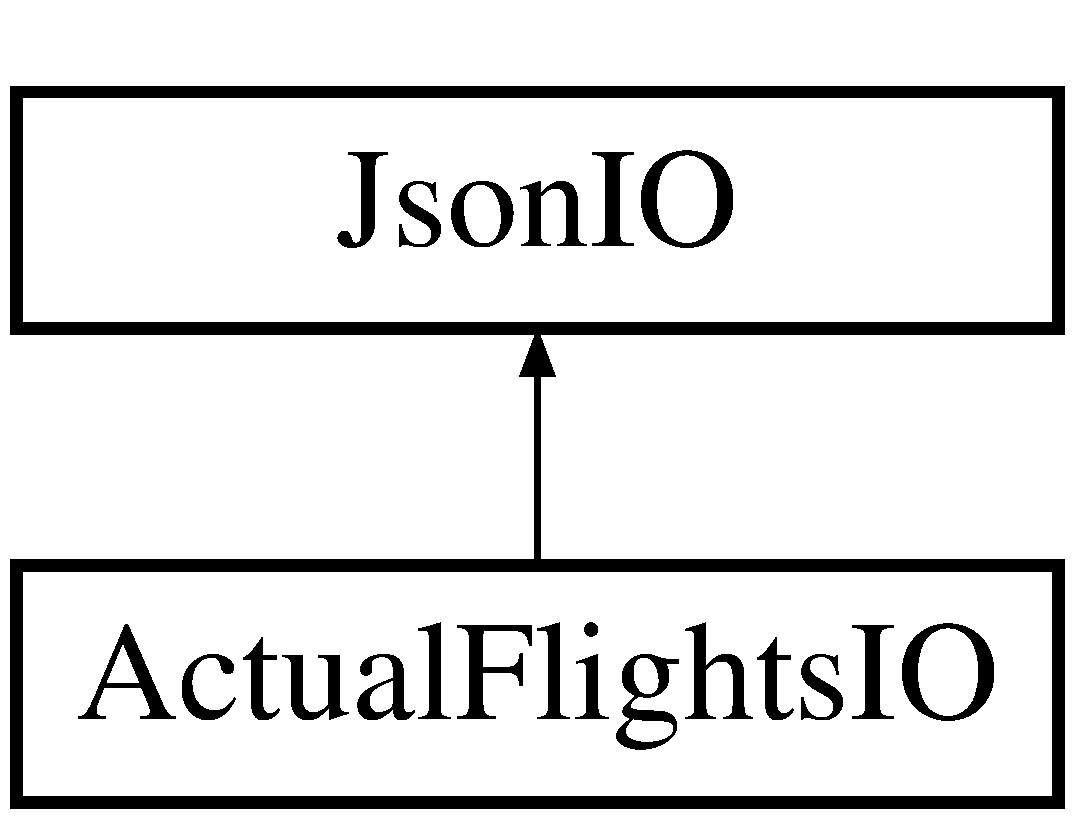
\includegraphics[height=2.000000cm]{class_actual_flights_i_o}
\end{center}
\end{figure}
\subsection*{Public Member Functions}
\begin{DoxyCompactItemize}
\item 
virtual void \hyperlink{class_actual_flights_i_o_a181dc53214b2e3d7d21c28d928e5f07b}{write\+File} (\hyperlink{class_json_1_1_value}{Json\+::\+Value} value)
\end{DoxyCompactItemize}
\subsection*{Static Public Member Functions}
\begin{DoxyCompactItemize}
\item 
static \hyperlink{class_json_1_1_value}{Json\+::\+Value} \hyperlink{class_actual_flights_i_o_ae69ccbdf62e74023d2e6bf71232a55f3}{read\+File} ()
\item 
static \hyperlink{class_json_1_1_value}{Json\+::\+Value} \hyperlink{class_actual_flights_i_o_a9ea172304485a41da1d8615878ffb93f}{get\+Actual\+Flights} ()
\item 
static std\+::vector$<$ \hyperlink{class_json_1_1_value}{Json\+::\+Value} $>$ \hyperlink{class_actual_flights_i_o_ae9529e787a486c0713df9351b77bb1f6}{get\+Actual\+Reports} ()
\end{DoxyCompactItemize}


\subsection{Detailed Description}
\hyperlink{class_actual_flights_i_o}{Actual\+Flights\+IO} is the utility library for reading and writing regarding the Actual\+Flights file. 

\subsection{Member Function Documentation}
\index{Actual\+Flights\+IO@{Actual\+Flights\+IO}!get\+Actual\+Flights@{get\+Actual\+Flights}}
\index{get\+Actual\+Flights@{get\+Actual\+Flights}!Actual\+Flights\+IO@{Actual\+Flights\+IO}}
\subsubsection[{\texorpdfstring{get\+Actual\+Flights()}{getActualFlights()}}]{\setlength{\rightskip}{0pt plus 5cm}{\bf Json\+::\+Value} Actual\+Flights\+I\+O\+::get\+Actual\+Flights (
\begin{DoxyParamCaption}
{}
\end{DoxyParamCaption}
)\hspace{0.3cm}{\ttfamily [static]}}\hypertarget{class_actual_flights_i_o_a9ea172304485a41da1d8615878ffb93f}{}\label{class_actual_flights_i_o_a9ea172304485a41da1d8615878ffb93f}
Reads the J\+S\+ON Actual\+Flights file and returns J\+S\+ON Value of Actual Flights. \begin{DoxyReturn}{Returns}
J\+S\+ON value of Actual Flights 
\end{DoxyReturn}
\index{Actual\+Flights\+IO@{Actual\+Flights\+IO}!get\+Actual\+Reports@{get\+Actual\+Reports}}
\index{get\+Actual\+Reports@{get\+Actual\+Reports}!Actual\+Flights\+IO@{Actual\+Flights\+IO}}
\subsubsection[{\texorpdfstring{get\+Actual\+Reports()}{getActualReports()}}]{\setlength{\rightskip}{0pt plus 5cm}std\+::vector$<$ {\bf Json\+::\+Value} $>$ Actual\+Flights\+I\+O\+::get\+Actual\+Reports (
\begin{DoxyParamCaption}
{}
\end{DoxyParamCaption}
)\hspace{0.3cm}{\ttfamily [static]}}\hypertarget{class_actual_flights_i_o_ae9529e787a486c0713df9351b77bb1f6}{}\label{class_actual_flights_i_o_ae9529e787a486c0713df9351b77bb1f6}
Gets a Vector containing all actual reports in the file. \begin{DoxyReturn}{Returns}
vector containing all the actual reports in \hyperlink{class_json_1_1_value}{Json\+::\+Value} form. 
\end{DoxyReturn}
\index{Actual\+Flights\+IO@{Actual\+Flights\+IO}!read\+File@{read\+File}}
\index{read\+File@{read\+File}!Actual\+Flights\+IO@{Actual\+Flights\+IO}}
\subsubsection[{\texorpdfstring{read\+File()}{readFile()}}]{\setlength{\rightskip}{0pt plus 5cm}{\bf Json\+::\+Value} Actual\+Flights\+I\+O\+::read\+File (
\begin{DoxyParamCaption}
{}
\end{DoxyParamCaption}
)\hspace{0.3cm}{\ttfamily [static]}}\hypertarget{class_actual_flights_i_o_ae69ccbdf62e74023d2e6bf71232a55f3}{}\label{class_actual_flights_i_o_ae69ccbdf62e74023d2e6bf71232a55f3}
Reads the J\+S\+ON Actual\+F\+Lights file and returns a reference to the root of the J\+S\+ON file. \begin{DoxyReturn}{Returns}
The root of the J\+S\+ON File 
\end{DoxyReturn}
\index{Actual\+Flights\+IO@{Actual\+Flights\+IO}!write\+File@{write\+File}}
\index{write\+File@{write\+File}!Actual\+Flights\+IO@{Actual\+Flights\+IO}}
\subsubsection[{\texorpdfstring{write\+File(\+Json\+::\+Value value)}{writeFile(Json::Value value)}}]{\setlength{\rightskip}{0pt plus 5cm}void Actual\+Flights\+I\+O\+::write\+File (
\begin{DoxyParamCaption}
\item[{{\bf Json\+::\+Value}}]{value}
\end{DoxyParamCaption}
)\hspace{0.3cm}{\ttfamily [virtual]}}\hypertarget{class_actual_flights_i_o_a181dc53214b2e3d7d21c28d928e5f07b}{}\label{class_actual_flights_i_o_a181dc53214b2e3d7d21c28d928e5f07b}
T\+O\+DO 

Implements \hyperlink{class_json_i_o}{Json\+IO}.



The documentation for this class was generated from the following files\+:\begin{DoxyCompactItemize}
\item 
/\+Users/\+Dat/\+Clion\+Projects/saas/lib/jsonio/inc/Actual\+Flights\+I\+O.\+h\item 
/\+Users/\+Dat/\+Clion\+Projects/saas/lib/jsonio/src/Actual\+Flights\+I\+O.\+cpp\end{DoxyCompactItemize}

\hypertarget{class_silent_orbit_1_1_protocol_buffers_1_1_allocation_stack}{}\section{Silent\+Orbit.\+Protocol\+Buffers.\+Allocation\+Stack Class Reference}
\label{class_silent_orbit_1_1_protocol_buffers_1_1_allocation_stack}\index{Silent\+Orbit.\+Protocol\+Buffers.\+Allocation\+Stack@{Silent\+Orbit.\+Protocol\+Buffers.\+Allocation\+Stack}}


Unoptimized stack, allocates a new Memory\+Stream for every request.  


Inheritance diagram for Silent\+Orbit.\+Protocol\+Buffers.\+Allocation\+Stack\+:\begin{figure}[H]
\begin{center}
\leavevmode
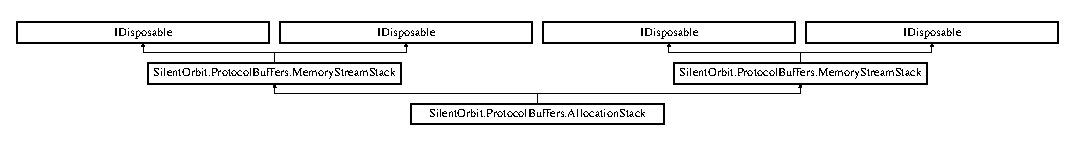
\includegraphics[height=1.443299cm]{class_silent_orbit_1_1_protocol_buffers_1_1_allocation_stack}
\end{center}
\end{figure}
\subsection*{Public Member Functions}
\begin{DoxyCompactItemize}
\item 
Memory\+Stream \hyperlink{class_silent_orbit_1_1_protocol_buffers_1_1_allocation_stack_afad82025096f48ada379e90d6651a5a2}{Pop} ()
\begin{DoxyCompactList}\small\item\em The returned stream is not reset. You must call .Set\+Length(0) before using it. This is done in the generated code. \end{DoxyCompactList}\item 
\hypertarget{class_silent_orbit_1_1_protocol_buffers_1_1_allocation_stack_a5c633c60b21b61c71f3bf8cec3e8dbe6}{}void {\bfseries Push} (Memory\+Stream stream)\label{class_silent_orbit_1_1_protocol_buffers_1_1_allocation_stack_a5c633c60b21b61c71f3bf8cec3e8dbe6}

\item 
\hypertarget{class_silent_orbit_1_1_protocol_buffers_1_1_allocation_stack_af84c205007df60160ddfe3cb0cff6725}{}void {\bfseries Dispose} ()\label{class_silent_orbit_1_1_protocol_buffers_1_1_allocation_stack_af84c205007df60160ddfe3cb0cff6725}

\item 
Memory\+Stream \hyperlink{class_silent_orbit_1_1_protocol_buffers_1_1_allocation_stack_afad82025096f48ada379e90d6651a5a2}{Pop} ()
\begin{DoxyCompactList}\small\item\em The returned stream is not reset. You must call .Set\+Length(0) before using it. This is done in the generated code. \end{DoxyCompactList}\item 
\hypertarget{class_silent_orbit_1_1_protocol_buffers_1_1_allocation_stack_a5c633c60b21b61c71f3bf8cec3e8dbe6}{}void {\bfseries Push} (Memory\+Stream stream)\label{class_silent_orbit_1_1_protocol_buffers_1_1_allocation_stack_a5c633c60b21b61c71f3bf8cec3e8dbe6}

\item 
\hypertarget{class_silent_orbit_1_1_protocol_buffers_1_1_allocation_stack_af84c205007df60160ddfe3cb0cff6725}{}void {\bfseries Dispose} ()\label{class_silent_orbit_1_1_protocol_buffers_1_1_allocation_stack_af84c205007df60160ddfe3cb0cff6725}

\end{DoxyCompactItemize}


\subsection{Detailed Description}
Unoptimized stack, allocates a new Memory\+Stream for every request. 



\subsection{Member Function Documentation}
\hypertarget{class_silent_orbit_1_1_protocol_buffers_1_1_allocation_stack_afad82025096f48ada379e90d6651a5a2}{}\index{Silent\+Orbit\+::\+Protocol\+Buffers\+::\+Allocation\+Stack@{Silent\+Orbit\+::\+Protocol\+Buffers\+::\+Allocation\+Stack}!Pop@{Pop}}
\index{Pop@{Pop}!Silent\+Orbit\+::\+Protocol\+Buffers\+::\+Allocation\+Stack@{Silent\+Orbit\+::\+Protocol\+Buffers\+::\+Allocation\+Stack}}
\subsubsection[{Pop}]{\setlength{\rightskip}{0pt plus 5cm}Memory\+Stream Silent\+Orbit.\+Protocol\+Buffers.\+Allocation\+Stack.\+Pop (
\begin{DoxyParamCaption}
{}
\end{DoxyParamCaption}
)\hspace{0.3cm}{\ttfamily [inline]}}\label{class_silent_orbit_1_1_protocol_buffers_1_1_allocation_stack_afad82025096f48ada379e90d6651a5a2}


The returned stream is not reset. You must call .Set\+Length(0) before using it. This is done in the generated code. 



Implements \hyperlink{interface_silent_orbit_1_1_protocol_buffers_1_1_memory_stream_stack}{Silent\+Orbit.\+Protocol\+Buffers.\+Memory\+Stream\+Stack}.

\hypertarget{class_silent_orbit_1_1_protocol_buffers_1_1_allocation_stack_afad82025096f48ada379e90d6651a5a2}{}\index{Silent\+Orbit\+::\+Protocol\+Buffers\+::\+Allocation\+Stack@{Silent\+Orbit\+::\+Protocol\+Buffers\+::\+Allocation\+Stack}!Pop@{Pop}}
\index{Pop@{Pop}!Silent\+Orbit\+::\+Protocol\+Buffers\+::\+Allocation\+Stack@{Silent\+Orbit\+::\+Protocol\+Buffers\+::\+Allocation\+Stack}}
\subsubsection[{Pop}]{\setlength{\rightskip}{0pt plus 5cm}Memory\+Stream Silent\+Orbit.\+Protocol\+Buffers.\+Allocation\+Stack.\+Pop (
\begin{DoxyParamCaption}
{}
\end{DoxyParamCaption}
)\hspace{0.3cm}{\ttfamily [inline]}}\label{class_silent_orbit_1_1_protocol_buffers_1_1_allocation_stack_afad82025096f48ada379e90d6651a5a2}


The returned stream is not reset. You must call .Set\+Length(0) before using it. This is done in the generated code. 



Implements \hyperlink{interface_silent_orbit_1_1_protocol_buffers_1_1_memory_stream_stack}{Silent\+Orbit.\+Protocol\+Buffers.\+Memory\+Stream\+Stack}.



The documentation for this class was generated from the following file\+:\begin{DoxyCompactItemize}
\item 
/home/fpoole/development/cpe406/saas/cdti/\+C\+D\+T\+I\+Unity/\+Assets/scripts/Protocol\+Parser.\+cs\end{DoxyCompactItemize}

\hypertarget{struct_json_1_1_built_styled_stream_writer}{}\section{Json\+:\+:Built\+Styled\+Stream\+Writer Struct Reference}
\label{struct_json_1_1_built_styled_stream_writer}\index{Json\+::\+Built\+Styled\+Stream\+Writer@{Json\+::\+Built\+Styled\+Stream\+Writer}}
Inheritance diagram for Json\+:\+:Built\+Styled\+Stream\+Writer\+:\begin{figure}[H]
\begin{center}
\leavevmode
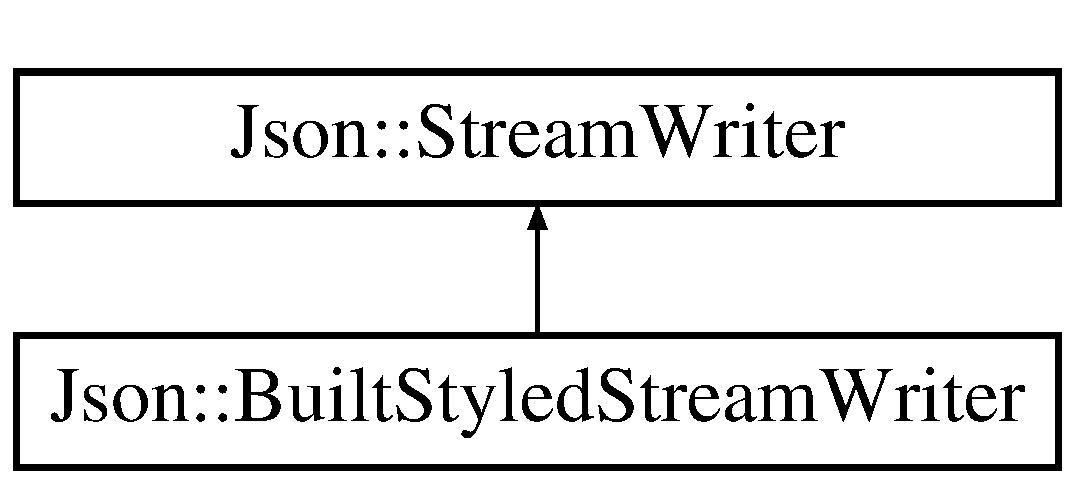
\includegraphics[height=2.000000cm]{struct_json_1_1_built_styled_stream_writer}
\end{center}
\end{figure}
\subsection*{Public Member Functions}
\begin{DoxyCompactItemize}
\item 
\hypertarget{struct_json_1_1_built_styled_stream_writer_ab0c2e665c86b22f8fafb0e52c8069954}{}{\bfseries Built\+Styled\+Stream\+Writer} (std\+::string const \&indentation, \hyperlink{struct_json_1_1_comment_style_a51fc08f3518fd81eba12f340d19a3d0c}{Comment\+Style\+::\+Enum} cs, std\+::string const \&colon\+Symbol, std\+::string const \&null\+Symbol, std\+::string const \&ending\+Line\+Feed\+Symbol, bool use\+Special\+Floats, unsigned int precision)\label{struct_json_1_1_built_styled_stream_writer_ab0c2e665c86b22f8fafb0e52c8069954}

\item 
int \hyperlink{struct_json_1_1_built_styled_stream_writer_a2ecffc3d66c4feddf208e5cd3b1c0f18}{write} (\hyperlink{class_json_1_1_value}{Value} const \&root, std\+::ostream $\ast$sout) override
\end{DoxyCompactItemize}
\subsection*{Additional Inherited Members}


\subsection{Member Function Documentation}
\hypertarget{struct_json_1_1_built_styled_stream_writer_a2ecffc3d66c4feddf208e5cd3b1c0f18}{}\index{Json\+::\+Built\+Styled\+Stream\+Writer@{Json\+::\+Built\+Styled\+Stream\+Writer}!write@{write}}
\index{write@{write}!Json\+::\+Built\+Styled\+Stream\+Writer@{Json\+::\+Built\+Styled\+Stream\+Writer}}
\subsubsection[{write}]{\setlength{\rightskip}{0pt plus 5cm}int Json\+::\+Built\+Styled\+Stream\+Writer\+::write (
\begin{DoxyParamCaption}
\item[{{\bf Value} const \&}]{root, }
\item[{std\+::ostream $\ast$}]{sout}
\end{DoxyParamCaption}
)\hspace{0.3cm}{\ttfamily [override]}, {\ttfamily [virtual]}}\label{struct_json_1_1_built_styled_stream_writer_a2ecffc3d66c4feddf208e5cd3b1c0f18}
Write \hyperlink{class_json_1_1_value}{Value} into document as configured in sub-\/class. Do not take ownership of sout, but maintain a reference during function. \begin{DoxyPrecond}{Precondition}
sout != N\+U\+L\+L 
\end{DoxyPrecond}
\begin{DoxyReturn}{Returns}
zero on success (For now, we always return zero, so check the stream instead.) 
\end{DoxyReturn}

\begin{DoxyExceptions}{Exceptions}
{\em std\+::exception} & possibly, depending on configuration \\
\hline
\end{DoxyExceptions}


Implements \hyperlink{class_json_1_1_stream_writer_a237368cf13b41decc015640d25f176ab}{Json\+::\+Stream\+Writer}.



The documentation for this struct was generated from the following file\+:\begin{DoxyCompactItemize}
\item 
/home/fpoole/development/cpe406/saas/lib/jsoncpp/src/jsoncpp.\+cpp\end{DoxyCompactItemize}

\hypertarget{class_example_1_1_c_d_t_i_plane}{}\section{Example.\+C\+D\+T\+I\+Plane Class Reference}
\label{class_example_1_1_c_d_t_i_plane}\index{Example.\+C\+D\+T\+I\+Plane@{Example.\+C\+D\+T\+I\+Plane}}


 


\subsection*{Public Types}
\begin{DoxyCompactItemize}
\item 
enum {\bfseries Severity} \{ {\bfseries P\+R\+O\+X\+I\+M\+A\+TE} = 0, 
{\bfseries T\+R\+A\+F\+F\+IC} = 1, 
{\bfseries R\+E\+S\+O\+L\+U\+T\+I\+ON} = 2
 \}\hypertarget{class_example_1_1_c_d_t_i_plane_af140920ed953b8579db5c8021fa03f92}{}\label{class_example_1_1_c_d_t_i_plane_af140920ed953b8579db5c8021fa03f92}

\end{DoxyCompactItemize}
\subsection*{Static Public Member Functions}
\begin{DoxyCompactItemize}
\item 
static \hyperlink{class_example_1_1_c_d_t_i_plane}{C\+D\+T\+I\+Plane} \hyperlink{class_example_1_1_c_d_t_i_plane_a9b57535386fd8416a21329193c1d4a8d}{Deserialize} (Stream stream)
\begin{DoxyCompactList}\small\item\em Helper\+: create a new instance to deserializing into\end{DoxyCompactList}\item 
static \hyperlink{class_example_1_1_c_d_t_i_plane}{C\+D\+T\+I\+Plane} \hyperlink{class_example_1_1_c_d_t_i_plane_a2a402540634e3e86a57af48860920f8c}{Deserialize\+Length\+Delimited} (Stream stream)
\begin{DoxyCompactList}\small\item\em Helper\+: create a new instance to deserializing into\end{DoxyCompactList}\item 
static \hyperlink{class_example_1_1_c_d_t_i_plane}{C\+D\+T\+I\+Plane} \hyperlink{class_example_1_1_c_d_t_i_plane_a60c2ac4412417d21c958f98f90424487}{Deserialize\+Length} (Stream stream, int length)
\begin{DoxyCompactList}\small\item\em Helper\+: create a new instance to deserializing into\end{DoxyCompactList}\item 
static \hyperlink{class_example_1_1_c_d_t_i_plane}{C\+D\+T\+I\+Plane} \hyperlink{class_example_1_1_c_d_t_i_plane_a4df1a00746b2efa5d9ecbea4a978ef6e}{Deserialize} (byte\mbox{[}$\,$\mbox{]} buffer)
\begin{DoxyCompactList}\small\item\em Helper\+: put the buffer into a Memory\+Stream and create a new instance to deserializing into\end{DoxyCompactList}\item 
static \hyperlink{class_example_1_1_c_d_t_i_plane}{Example.\+C\+D\+T\+I\+Plane} \hyperlink{class_example_1_1_c_d_t_i_plane_a82f32570c03dea0189e0f31acb7f8d0c}{Deserialize} (byte\mbox{[}$\,$\mbox{]} buffer, \hyperlink{class_example_1_1_c_d_t_i_plane}{Example.\+C\+D\+T\+I\+Plane} instance)
\begin{DoxyCompactList}\small\item\em Helper\+: put the buffer into a Memory\+Stream before deserializing\end{DoxyCompactList}\item 
static \hyperlink{class_example_1_1_c_d_t_i_plane}{Example.\+C\+D\+T\+I\+Plane} \hyperlink{class_example_1_1_c_d_t_i_plane_ad4231bb21fad192ec5235136c7efc2f3}{Deserialize} (Stream stream, \hyperlink{class_example_1_1_c_d_t_i_plane}{Example.\+C\+D\+T\+I\+Plane} instance)
\begin{DoxyCompactList}\small\item\em Takes the remaining content of the stream and deserialze it into the instance.\end{DoxyCompactList}\item 
static \hyperlink{class_example_1_1_c_d_t_i_plane}{Example.\+C\+D\+T\+I\+Plane} \hyperlink{class_example_1_1_c_d_t_i_plane_ae2f44dc0c44f735cb4d8cc977d5a8e01}{Deserialize\+Length\+Delimited} (Stream stream, \hyperlink{class_example_1_1_c_d_t_i_plane}{Example.\+C\+D\+T\+I\+Plane} instance)
\begin{DoxyCompactList}\small\item\em Read the Var\+Int length prefix and the given number of bytes from the stream and deserialze it into the instance.\end{DoxyCompactList}\item 
static \hyperlink{class_example_1_1_c_d_t_i_plane}{Example.\+C\+D\+T\+I\+Plane} \hyperlink{class_example_1_1_c_d_t_i_plane_a0a9d43348ee794a421d41c1fe66865db}{Deserialize\+Length} (Stream stream, int length, \hyperlink{class_example_1_1_c_d_t_i_plane}{Example.\+C\+D\+T\+I\+Plane} instance)
\begin{DoxyCompactList}\small\item\em Read the given number of bytes from the stream and deserialze it into the instance.\end{DoxyCompactList}\item 
static void \hyperlink{class_example_1_1_c_d_t_i_plane_a56aa1ceb3a4ad073c405dd9fad2bdc57}{Serialize} (Stream stream, \hyperlink{class_example_1_1_c_d_t_i_plane}{C\+D\+T\+I\+Plane} instance)
\begin{DoxyCompactList}\small\item\em Serialize the instance into the stream\end{DoxyCompactList}\item 
static byte\mbox{[}$\,$\mbox{]} \hyperlink{class_example_1_1_c_d_t_i_plane_a6de7c84b310e228f607f6dc5ed9ed3e3}{Serialize\+To\+Bytes} (\hyperlink{class_example_1_1_c_d_t_i_plane}{C\+D\+T\+I\+Plane} instance)
\begin{DoxyCompactList}\small\item\em Helper\+: Serialize into a Memory\+Stream and return its byte array\end{DoxyCompactList}\item 
static void \hyperlink{class_example_1_1_c_d_t_i_plane_a861c8211cc2b5f3bcaf3721dff13435c}{Serialize\+Length\+Delimited} (Stream stream, \hyperlink{class_example_1_1_c_d_t_i_plane}{C\+D\+T\+I\+Plane} instance)
\begin{DoxyCompactList}\small\item\em Helper\+: Serialize with a varint length prefix\end{DoxyCompactList}\end{DoxyCompactItemize}
\subsection*{Properties}
\begin{DoxyCompactItemize}
\item 
string {\bfseries Id}\hspace{0.3cm}{\ttfamily  \mbox{[}get, set\mbox{]}}\hypertarget{class_example_1_1_c_d_t_i_plane_a95d3fc498b17a8d92557081390424550}{}\label{class_example_1_1_c_d_t_i_plane_a95d3fc498b17a8d92557081390424550}

\item 
\hyperlink{class_example_1_1_vector}{Example.\+Vector} \hyperlink{class_example_1_1_c_d_t_i_plane_a4d6766b3ddf6726e0b6beda5f7044f39}{Position}\hspace{0.3cm}{\ttfamily  \mbox{[}get, set\mbox{]}}
\begin{DoxyCompactList}\small\item\em ID of target\end{DoxyCompactList}\item 
\hyperlink{class_example_1_1_vector}{Example.\+Vector} \hyperlink{class_example_1_1_c_d_t_i_plane_a52e1d4c9df3e1b3b5f281bbac9e49269}{Velocity}\hspace{0.3cm}{\ttfamily  \mbox{[}get, set\mbox{]}}
\item 
Example.\+C\+D\+T\+I\+Plane.\+Severity \hyperlink{class_example_1_1_c_d_t_i_plane_ac51cdc50b63036c15eb1dc03f9d8369c}{severity}\hspace{0.3cm}{\ttfamily  \mbox{[}get, set\mbox{]}}
\begin{DoxyCompactList}\small\item\em North East and Down, in Feet/\+Second\end{DoxyCompactList}\end{DoxyCompactItemize}


\subsection{Detailed Description}


$\ast$

$\ast$ Represents one plane in the C\+D\+TI message.

\subsection{Member Function Documentation}
\index{Example\+::\+C\+D\+T\+I\+Plane@{Example\+::\+C\+D\+T\+I\+Plane}!Deserialize@{Deserialize}}
\index{Deserialize@{Deserialize}!Example\+::\+C\+D\+T\+I\+Plane@{Example\+::\+C\+D\+T\+I\+Plane}}
\subsubsection[{\texorpdfstring{Deserialize(\+Stream stream)}{Deserialize(Stream stream)}}]{\setlength{\rightskip}{0pt plus 5cm}static {\bf C\+D\+T\+I\+Plane} Example.\+C\+D\+T\+I\+Plane.\+Deserialize (
\begin{DoxyParamCaption}
\item[{Stream}]{stream}
\end{DoxyParamCaption}
)\hspace{0.3cm}{\ttfamily [inline]}, {\ttfamily [static]}}\hypertarget{class_example_1_1_c_d_t_i_plane_a9b57535386fd8416a21329193c1d4a8d}{}\label{class_example_1_1_c_d_t_i_plane_a9b57535386fd8416a21329193c1d4a8d}


Helper\+: create a new instance to deserializing into

\index{Example\+::\+C\+D\+T\+I\+Plane@{Example\+::\+C\+D\+T\+I\+Plane}!Deserialize@{Deserialize}}
\index{Deserialize@{Deserialize}!Example\+::\+C\+D\+T\+I\+Plane@{Example\+::\+C\+D\+T\+I\+Plane}}
\subsubsection[{\texorpdfstring{Deserialize(byte[] buffer)}{Deserialize(byte[] buffer)}}]{\setlength{\rightskip}{0pt plus 5cm}static {\bf C\+D\+T\+I\+Plane} Example.\+C\+D\+T\+I\+Plane.\+Deserialize (
\begin{DoxyParamCaption}
\item[{byte\mbox{[}$\,$\mbox{]}}]{buffer}
\end{DoxyParamCaption}
)\hspace{0.3cm}{\ttfamily [inline]}, {\ttfamily [static]}}\hypertarget{class_example_1_1_c_d_t_i_plane_a4df1a00746b2efa5d9ecbea4a978ef6e}{}\label{class_example_1_1_c_d_t_i_plane_a4df1a00746b2efa5d9ecbea4a978ef6e}


Helper\+: put the buffer into a Memory\+Stream and create a new instance to deserializing into

\index{Example\+::\+C\+D\+T\+I\+Plane@{Example\+::\+C\+D\+T\+I\+Plane}!Deserialize@{Deserialize}}
\index{Deserialize@{Deserialize}!Example\+::\+C\+D\+T\+I\+Plane@{Example\+::\+C\+D\+T\+I\+Plane}}
\subsubsection[{\texorpdfstring{Deserialize(byte[] buffer, Example.\+C\+D\+T\+I\+Plane instance)}{Deserialize(byte[] buffer, Example.CDTIPlane instance)}}]{\setlength{\rightskip}{0pt plus 5cm}static {\bf Example.\+C\+D\+T\+I\+Plane} Example.\+C\+D\+T\+I\+Plane.\+Deserialize (
\begin{DoxyParamCaption}
\item[{byte\mbox{[}$\,$\mbox{]}}]{buffer, }
\item[{{\bf Example.\+C\+D\+T\+I\+Plane}}]{instance}
\end{DoxyParamCaption}
)\hspace{0.3cm}{\ttfamily [inline]}, {\ttfamily [static]}}\hypertarget{class_example_1_1_c_d_t_i_plane_a82f32570c03dea0189e0f31acb7f8d0c}{}\label{class_example_1_1_c_d_t_i_plane_a82f32570c03dea0189e0f31acb7f8d0c}


Helper\+: put the buffer into a Memory\+Stream before deserializing

\index{Example\+::\+C\+D\+T\+I\+Plane@{Example\+::\+C\+D\+T\+I\+Plane}!Deserialize@{Deserialize}}
\index{Deserialize@{Deserialize}!Example\+::\+C\+D\+T\+I\+Plane@{Example\+::\+C\+D\+T\+I\+Plane}}
\subsubsection[{\texorpdfstring{Deserialize(\+Stream stream, Example.\+C\+D\+T\+I\+Plane instance)}{Deserialize(Stream stream, Example.CDTIPlane instance)}}]{\setlength{\rightskip}{0pt plus 5cm}static {\bf Example.\+C\+D\+T\+I\+Plane} Example.\+C\+D\+T\+I\+Plane.\+Deserialize (
\begin{DoxyParamCaption}
\item[{Stream}]{stream, }
\item[{{\bf Example.\+C\+D\+T\+I\+Plane}}]{instance}
\end{DoxyParamCaption}
)\hspace{0.3cm}{\ttfamily [inline]}, {\ttfamily [static]}}\hypertarget{class_example_1_1_c_d_t_i_plane_ad4231bb21fad192ec5235136c7efc2f3}{}\label{class_example_1_1_c_d_t_i_plane_ad4231bb21fad192ec5235136c7efc2f3}


Takes the remaining content of the stream and deserialze it into the instance.

\index{Example\+::\+C\+D\+T\+I\+Plane@{Example\+::\+C\+D\+T\+I\+Plane}!Deserialize\+Length@{Deserialize\+Length}}
\index{Deserialize\+Length@{Deserialize\+Length}!Example\+::\+C\+D\+T\+I\+Plane@{Example\+::\+C\+D\+T\+I\+Plane}}
\subsubsection[{\texorpdfstring{Deserialize\+Length(\+Stream stream, int length)}{DeserializeLength(Stream stream, int length)}}]{\setlength{\rightskip}{0pt plus 5cm}static {\bf C\+D\+T\+I\+Plane} Example.\+C\+D\+T\+I\+Plane.\+Deserialize\+Length (
\begin{DoxyParamCaption}
\item[{Stream}]{stream, }
\item[{int}]{length}
\end{DoxyParamCaption}
)\hspace{0.3cm}{\ttfamily [inline]}, {\ttfamily [static]}}\hypertarget{class_example_1_1_c_d_t_i_plane_a60c2ac4412417d21c958f98f90424487}{}\label{class_example_1_1_c_d_t_i_plane_a60c2ac4412417d21c958f98f90424487}


Helper\+: create a new instance to deserializing into

\index{Example\+::\+C\+D\+T\+I\+Plane@{Example\+::\+C\+D\+T\+I\+Plane}!Deserialize\+Length@{Deserialize\+Length}}
\index{Deserialize\+Length@{Deserialize\+Length}!Example\+::\+C\+D\+T\+I\+Plane@{Example\+::\+C\+D\+T\+I\+Plane}}
\subsubsection[{\texorpdfstring{Deserialize\+Length(\+Stream stream, int length, Example.\+C\+D\+T\+I\+Plane instance)}{DeserializeLength(Stream stream, int length, Example.CDTIPlane instance)}}]{\setlength{\rightskip}{0pt plus 5cm}static {\bf Example.\+C\+D\+T\+I\+Plane} Example.\+C\+D\+T\+I\+Plane.\+Deserialize\+Length (
\begin{DoxyParamCaption}
\item[{Stream}]{stream, }
\item[{int}]{length, }
\item[{{\bf Example.\+C\+D\+T\+I\+Plane}}]{instance}
\end{DoxyParamCaption}
)\hspace{0.3cm}{\ttfamily [inline]}, {\ttfamily [static]}}\hypertarget{class_example_1_1_c_d_t_i_plane_a0a9d43348ee794a421d41c1fe66865db}{}\label{class_example_1_1_c_d_t_i_plane_a0a9d43348ee794a421d41c1fe66865db}


Read the given number of bytes from the stream and deserialze it into the instance.

\index{Example\+::\+C\+D\+T\+I\+Plane@{Example\+::\+C\+D\+T\+I\+Plane}!Deserialize\+Length\+Delimited@{Deserialize\+Length\+Delimited}}
\index{Deserialize\+Length\+Delimited@{Deserialize\+Length\+Delimited}!Example\+::\+C\+D\+T\+I\+Plane@{Example\+::\+C\+D\+T\+I\+Plane}}
\subsubsection[{\texorpdfstring{Deserialize\+Length\+Delimited(\+Stream stream)}{DeserializeLengthDelimited(Stream stream)}}]{\setlength{\rightskip}{0pt plus 5cm}static {\bf C\+D\+T\+I\+Plane} Example.\+C\+D\+T\+I\+Plane.\+Deserialize\+Length\+Delimited (
\begin{DoxyParamCaption}
\item[{Stream}]{stream}
\end{DoxyParamCaption}
)\hspace{0.3cm}{\ttfamily [inline]}, {\ttfamily [static]}}\hypertarget{class_example_1_1_c_d_t_i_plane_a2a402540634e3e86a57af48860920f8c}{}\label{class_example_1_1_c_d_t_i_plane_a2a402540634e3e86a57af48860920f8c}


Helper\+: create a new instance to deserializing into

\index{Example\+::\+C\+D\+T\+I\+Plane@{Example\+::\+C\+D\+T\+I\+Plane}!Deserialize\+Length\+Delimited@{Deserialize\+Length\+Delimited}}
\index{Deserialize\+Length\+Delimited@{Deserialize\+Length\+Delimited}!Example\+::\+C\+D\+T\+I\+Plane@{Example\+::\+C\+D\+T\+I\+Plane}}
\subsubsection[{\texorpdfstring{Deserialize\+Length\+Delimited(\+Stream stream, Example.\+C\+D\+T\+I\+Plane instance)}{DeserializeLengthDelimited(Stream stream, Example.CDTIPlane instance)}}]{\setlength{\rightskip}{0pt plus 5cm}static {\bf Example.\+C\+D\+T\+I\+Plane} Example.\+C\+D\+T\+I\+Plane.\+Deserialize\+Length\+Delimited (
\begin{DoxyParamCaption}
\item[{Stream}]{stream, }
\item[{{\bf Example.\+C\+D\+T\+I\+Plane}}]{instance}
\end{DoxyParamCaption}
)\hspace{0.3cm}{\ttfamily [inline]}, {\ttfamily [static]}}\hypertarget{class_example_1_1_c_d_t_i_plane_ae2f44dc0c44f735cb4d8cc977d5a8e01}{}\label{class_example_1_1_c_d_t_i_plane_ae2f44dc0c44f735cb4d8cc977d5a8e01}


Read the Var\+Int length prefix and the given number of bytes from the stream and deserialze it into the instance.

\index{Example\+::\+C\+D\+T\+I\+Plane@{Example\+::\+C\+D\+T\+I\+Plane}!Serialize@{Serialize}}
\index{Serialize@{Serialize}!Example\+::\+C\+D\+T\+I\+Plane@{Example\+::\+C\+D\+T\+I\+Plane}}
\subsubsection[{\texorpdfstring{Serialize(\+Stream stream, C\+D\+T\+I\+Plane instance)}{Serialize(Stream stream, CDTIPlane instance)}}]{\setlength{\rightskip}{0pt plus 5cm}static void Example.\+C\+D\+T\+I\+Plane.\+Serialize (
\begin{DoxyParamCaption}
\item[{Stream}]{stream, }
\item[{{\bf C\+D\+T\+I\+Plane}}]{instance}
\end{DoxyParamCaption}
)\hspace{0.3cm}{\ttfamily [inline]}, {\ttfamily [static]}}\hypertarget{class_example_1_1_c_d_t_i_plane_a56aa1ceb3a4ad073c405dd9fad2bdc57}{}\label{class_example_1_1_c_d_t_i_plane_a56aa1ceb3a4ad073c405dd9fad2bdc57}


Serialize the instance into the stream

\index{Example\+::\+C\+D\+T\+I\+Plane@{Example\+::\+C\+D\+T\+I\+Plane}!Serialize\+Length\+Delimited@{Serialize\+Length\+Delimited}}
\index{Serialize\+Length\+Delimited@{Serialize\+Length\+Delimited}!Example\+::\+C\+D\+T\+I\+Plane@{Example\+::\+C\+D\+T\+I\+Plane}}
\subsubsection[{\texorpdfstring{Serialize\+Length\+Delimited(\+Stream stream, C\+D\+T\+I\+Plane instance)}{SerializeLengthDelimited(Stream stream, CDTIPlane instance)}}]{\setlength{\rightskip}{0pt plus 5cm}static void Example.\+C\+D\+T\+I\+Plane.\+Serialize\+Length\+Delimited (
\begin{DoxyParamCaption}
\item[{Stream}]{stream, }
\item[{{\bf C\+D\+T\+I\+Plane}}]{instance}
\end{DoxyParamCaption}
)\hspace{0.3cm}{\ttfamily [inline]}, {\ttfamily [static]}}\hypertarget{class_example_1_1_c_d_t_i_plane_a861c8211cc2b5f3bcaf3721dff13435c}{}\label{class_example_1_1_c_d_t_i_plane_a861c8211cc2b5f3bcaf3721dff13435c}


Helper\+: Serialize with a varint length prefix

\index{Example\+::\+C\+D\+T\+I\+Plane@{Example\+::\+C\+D\+T\+I\+Plane}!Serialize\+To\+Bytes@{Serialize\+To\+Bytes}}
\index{Serialize\+To\+Bytes@{Serialize\+To\+Bytes}!Example\+::\+C\+D\+T\+I\+Plane@{Example\+::\+C\+D\+T\+I\+Plane}}
\subsubsection[{\texorpdfstring{Serialize\+To\+Bytes(\+C\+D\+T\+I\+Plane instance)}{SerializeToBytes(CDTIPlane instance)}}]{\setlength{\rightskip}{0pt plus 5cm}static byte \mbox{[}$\,$\mbox{]} Example.\+C\+D\+T\+I\+Plane.\+Serialize\+To\+Bytes (
\begin{DoxyParamCaption}
\item[{{\bf C\+D\+T\+I\+Plane}}]{instance}
\end{DoxyParamCaption}
)\hspace{0.3cm}{\ttfamily [inline]}, {\ttfamily [static]}}\hypertarget{class_example_1_1_c_d_t_i_plane_a6de7c84b310e228f607f6dc5ed9ed3e3}{}\label{class_example_1_1_c_d_t_i_plane_a6de7c84b310e228f607f6dc5ed9ed3e3}


Helper\+: Serialize into a Memory\+Stream and return its byte array



\subsection{Property Documentation}
\index{Example\+::\+C\+D\+T\+I\+Plane@{Example\+::\+C\+D\+T\+I\+Plane}!Position@{Position}}
\index{Position@{Position}!Example\+::\+C\+D\+T\+I\+Plane@{Example\+::\+C\+D\+T\+I\+Plane}}
\subsubsection[{\texorpdfstring{Position}{Position}}]{\setlength{\rightskip}{0pt plus 5cm}{\bf Example.\+Vector} Example.\+C\+D\+T\+I\+Plane.\+Position\hspace{0.3cm}{\ttfamily [get]}, {\ttfamily [set]}}\hypertarget{class_example_1_1_c_d_t_i_plane_a4d6766b3ddf6726e0b6beda5f7044f39}{}\label{class_example_1_1_c_d_t_i_plane_a4d6766b3ddf6726e0b6beda5f7044f39}


ID of target

\index{Example\+::\+C\+D\+T\+I\+Plane@{Example\+::\+C\+D\+T\+I\+Plane}!severity@{severity}}
\index{severity@{severity}!Example\+::\+C\+D\+T\+I\+Plane@{Example\+::\+C\+D\+T\+I\+Plane}}
\subsubsection[{\texorpdfstring{severity}{severity}}]{\setlength{\rightskip}{0pt plus 5cm}Example.\+C\+D\+T\+I\+Plane.\+Severity Example.\+C\+D\+T\+I\+Plane.\+severity\hspace{0.3cm}{\ttfamily [get]}, {\ttfamily [set]}}\hypertarget{class_example_1_1_c_d_t_i_plane_ac51cdc50b63036c15eb1dc03f9d8369c}{}\label{class_example_1_1_c_d_t_i_plane_ac51cdc50b63036c15eb1dc03f9d8369c}


North East and Down, in Feet/\+Second

\index{Example\+::\+C\+D\+T\+I\+Plane@{Example\+::\+C\+D\+T\+I\+Plane}!Velocity@{Velocity}}
\index{Velocity@{Velocity}!Example\+::\+C\+D\+T\+I\+Plane@{Example\+::\+C\+D\+T\+I\+Plane}}
\subsubsection[{\texorpdfstring{Velocity}{Velocity}}]{\setlength{\rightskip}{0pt plus 5cm}{\bf Example.\+Vector} Example.\+C\+D\+T\+I\+Plane.\+Velocity\hspace{0.3cm}{\ttfamily [get]}, {\ttfamily [set]}}\hypertarget{class_example_1_1_c_d_t_i_plane_a52e1d4c9df3e1b3b5f281bbac9e49269}{}\label{class_example_1_1_c_d_t_i_plane_a52e1d4c9df3e1b3b5f281bbac9e49269}




Relative to Ownship.

X and Y are in Nautical Miles, Z is in feet

The documentation for this class was generated from the following files\+:\begin{DoxyCompactItemize}
\item 
/\+Users/\+Dat/\+Clion\+Projects/saas/cdti/\+C\+D\+T\+I\+Unity/\+Assets/scripts/cdti.\+cs\item 
/\+Users/\+Dat/\+Clion\+Projects/saas/cdti/\+C\+D\+T\+I\+Unity/\+Assets/scripts/cdti.\+Serializer.\+cs\end{DoxyCompactItemize}

\hypertarget{class_example_1_1_c_d_t_i_report}{}\section{Example.\+C\+D\+T\+I\+Report Class Reference}
\label{class_example_1_1_c_d_t_i_report}\index{Example.\+C\+D\+T\+I\+Report@{Example.\+C\+D\+T\+I\+Report}}


 


\subsection*{Public Types}
\begin{DoxyCompactItemize}
\item 
\hypertarget{class_example_1_1_c_d_t_i_report_a2e9a6b1d49e40e4ef91e4f51f7cb56be}{}enum {\bfseries Severity} \{ {\bfseries P\+R\+O\+X\+I\+M\+A\+T\+E} = 0, 
{\bfseries T\+R\+A\+F\+F\+I\+C} = 1, 
{\bfseries R\+E\+S\+O\+L\+U\+T\+I\+O\+N} = 2
 \}\label{class_example_1_1_c_d_t_i_report_a2e9a6b1d49e40e4ef91e4f51f7cb56be}

\end{DoxyCompactItemize}
\subsection*{Static Public Member Functions}
\begin{DoxyCompactItemize}
\item 
static \hyperlink{class_example_1_1_c_d_t_i_report}{C\+D\+T\+I\+Report} \hyperlink{class_example_1_1_c_d_t_i_report_ac839a59baea94b2d0d85e233f0afaf31}{Deserialize} (Stream stream)
\begin{DoxyCompactList}\small\item\em Helper\+: create a new instance to deserializing into\end{DoxyCompactList}\item 
static \hyperlink{class_example_1_1_c_d_t_i_report}{C\+D\+T\+I\+Report} \hyperlink{class_example_1_1_c_d_t_i_report_a6e790e0e071fac05495f369414a8131a}{Deserialize\+Length\+Delimited} (Stream stream)
\begin{DoxyCompactList}\small\item\em Helper\+: create a new instance to deserializing into\end{DoxyCompactList}\item 
static \hyperlink{class_example_1_1_c_d_t_i_report}{C\+D\+T\+I\+Report} \hyperlink{class_example_1_1_c_d_t_i_report_a12c67ba955b64011c831c1f9b3f64f07}{Deserialize\+Length} (Stream stream, int length)
\begin{DoxyCompactList}\small\item\em Helper\+: create a new instance to deserializing into\end{DoxyCompactList}\item 
static \hyperlink{class_example_1_1_c_d_t_i_report}{C\+D\+T\+I\+Report} \hyperlink{class_example_1_1_c_d_t_i_report_a7ef6d83b62dd2beac045403f6e1a8054}{Deserialize} (byte\mbox{[}$\,$\mbox{]} buffer)
\begin{DoxyCompactList}\small\item\em Helper\+: put the buffer into a Memory\+Stream and create a new instance to deserializing into\end{DoxyCompactList}\item 
static \hyperlink{class_example_1_1_c_d_t_i_report}{Example.\+C\+D\+T\+I\+Report} \hyperlink{class_example_1_1_c_d_t_i_report_a858fd88fb0a1f98ee24f1ddd1d43e3e0}{Deserialize} (byte\mbox{[}$\,$\mbox{]} buffer, \hyperlink{class_example_1_1_c_d_t_i_report}{Example.\+C\+D\+T\+I\+Report} instance)
\begin{DoxyCompactList}\small\item\em Helper\+: put the buffer into a Memory\+Stream before deserializing\end{DoxyCompactList}\item 
static \hyperlink{class_example_1_1_c_d_t_i_report}{Example.\+C\+D\+T\+I\+Report} \hyperlink{class_example_1_1_c_d_t_i_report_a3259ef658ecda5587d8f394849544307}{Deserialize} (Stream stream, \hyperlink{class_example_1_1_c_d_t_i_report}{Example.\+C\+D\+T\+I\+Report} instance)
\begin{DoxyCompactList}\small\item\em Takes the remaining content of the stream and deserialze it into the instance.\end{DoxyCompactList}\item 
static \hyperlink{class_example_1_1_c_d_t_i_report}{Example.\+C\+D\+T\+I\+Report} \hyperlink{class_example_1_1_c_d_t_i_report_a837fd35c86c5ecd43a9ec5b149a37c2b}{Deserialize\+Length\+Delimited} (Stream stream, \hyperlink{class_example_1_1_c_d_t_i_report}{Example.\+C\+D\+T\+I\+Report} instance)
\begin{DoxyCompactList}\small\item\em Read the Var\+Int length prefix and the given number of bytes from the stream and deserialze it into the instance.\end{DoxyCompactList}\item 
static \hyperlink{class_example_1_1_c_d_t_i_report}{Example.\+C\+D\+T\+I\+Report} \hyperlink{class_example_1_1_c_d_t_i_report_a6842f35b509032e593cac6721c53dc3f}{Deserialize\+Length} (Stream stream, int length, \hyperlink{class_example_1_1_c_d_t_i_report}{Example.\+C\+D\+T\+I\+Report} instance)
\begin{DoxyCompactList}\small\item\em Read the given number of bytes from the stream and deserialze it into the instance.\end{DoxyCompactList}\item 
static void \hyperlink{class_example_1_1_c_d_t_i_report_aa35a297b34ae5b717ad4a35b3d43dfaf}{Serialize} (Stream stream, \hyperlink{class_example_1_1_c_d_t_i_report}{C\+D\+T\+I\+Report} instance)
\begin{DoxyCompactList}\small\item\em Serialize the instance into the stream\end{DoxyCompactList}\item 
static byte\mbox{[}$\,$\mbox{]} \hyperlink{class_example_1_1_c_d_t_i_report_a45ad424e439e8f5cea9306fdf40886ba}{Serialize\+To\+Bytes} (\hyperlink{class_example_1_1_c_d_t_i_report}{C\+D\+T\+I\+Report} instance)
\begin{DoxyCompactList}\small\item\em Helper\+: Serialize into a Memory\+Stream and return its byte array\end{DoxyCompactList}\item 
static void \hyperlink{class_example_1_1_c_d_t_i_report_a587ec4906faa62164e4dd7106ab43172}{Serialize\+Length\+Delimited} (Stream stream, \hyperlink{class_example_1_1_c_d_t_i_report}{C\+D\+T\+I\+Report} instance)
\begin{DoxyCompactList}\small\item\em Helper\+: Serialize with a varint length prefix\end{DoxyCompactList}\end{DoxyCompactItemize}
\subsection*{Properties}
\begin{DoxyCompactItemize}
\item 
\hypertarget{class_example_1_1_c_d_t_i_report_aa757cb6e78cfd34982eecc6f381c5450}{}long {\bfseries Timestamp}\hspace{0.3cm}{\ttfamily  \mbox{[}get, set\mbox{]}}\label{class_example_1_1_c_d_t_i_report_aa757cb6e78cfd34982eecc6f381c5450}

\item 
\hyperlink{class_example_1_1_c_d_t_i_plane}{Example.\+C\+D\+T\+I\+Plane} \hyperlink{class_example_1_1_c_d_t_i_report_ad40efe2d19d10dabc930320ba2835337}{Ownship}\hspace{0.3cm}{\ttfamily  \mbox{[}get, set\mbox{]}}
\begin{DoxyCompactList}\small\item\em U\+T\+C timestamp\end{DoxyCompactList}\item 
string \hyperlink{class_example_1_1_c_d_t_i_report_a6859a3fc5d356d9125d589e23a6cc2b9}{Advisory\+Message}\hspace{0.3cm}{\ttfamily  \mbox{[}get, set\mbox{]}}
\begin{DoxyCompactList}\small\item\em Ownship id and velocity, position is 0\end{DoxyCompactList}\item 
Example.\+C\+D\+T\+I\+Report.\+Severity \hyperlink{class_example_1_1_c_d_t_i_report_a55ef7e8b3e35eeeb0b273fd3c475ba31}{Advisory\+Level}\hspace{0.3cm}{\ttfamily  \mbox{[}get, set\mbox{]}}
\begin{DoxyCompactList}\small\item\em The string to display\end{DoxyCompactList}\item 
List$<$ \hyperlink{class_example_1_1_c_d_t_i_plane}{Example.\+C\+D\+T\+I\+Plane} $>$ \hyperlink{class_example_1_1_c_d_t_i_report_a73959c38addf562d6b64ecb538db006a}{Planes}\hspace{0.3cm}{\ttfamily  \mbox{[}get, set\mbox{]}}
\begin{DoxyCompactList}\small\item\em The warning level\end{DoxyCompactList}\end{DoxyCompactItemize}


\subsection{Detailed Description}


$\ast$

$\ast$ C\+D\+T\+I Report, sent once a second by the S\+A\+A application.

$\ast$ Contains a list of planes, and an optional message.

\subsection{Member Function Documentation}
\hypertarget{class_example_1_1_c_d_t_i_report_ac839a59baea94b2d0d85e233f0afaf31}{}\index{Example\+::\+C\+D\+T\+I\+Report@{Example\+::\+C\+D\+T\+I\+Report}!Deserialize@{Deserialize}}
\index{Deserialize@{Deserialize}!Example\+::\+C\+D\+T\+I\+Report@{Example\+::\+C\+D\+T\+I\+Report}}
\subsubsection[{Deserialize}]{\setlength{\rightskip}{0pt plus 5cm}static {\bf C\+D\+T\+I\+Report} Example.\+C\+D\+T\+I\+Report.\+Deserialize (
\begin{DoxyParamCaption}
\item[{Stream}]{stream}
\end{DoxyParamCaption}
)\hspace{0.3cm}{\ttfamily [inline]}, {\ttfamily [static]}}\label{class_example_1_1_c_d_t_i_report_ac839a59baea94b2d0d85e233f0afaf31}


Helper\+: create a new instance to deserializing into

\hypertarget{class_example_1_1_c_d_t_i_report_a7ef6d83b62dd2beac045403f6e1a8054}{}\index{Example\+::\+C\+D\+T\+I\+Report@{Example\+::\+C\+D\+T\+I\+Report}!Deserialize@{Deserialize}}
\index{Deserialize@{Deserialize}!Example\+::\+C\+D\+T\+I\+Report@{Example\+::\+C\+D\+T\+I\+Report}}
\subsubsection[{Deserialize}]{\setlength{\rightskip}{0pt plus 5cm}static {\bf C\+D\+T\+I\+Report} Example.\+C\+D\+T\+I\+Report.\+Deserialize (
\begin{DoxyParamCaption}
\item[{byte\mbox{[}$\,$\mbox{]}}]{buffer}
\end{DoxyParamCaption}
)\hspace{0.3cm}{\ttfamily [inline]}, {\ttfamily [static]}}\label{class_example_1_1_c_d_t_i_report_a7ef6d83b62dd2beac045403f6e1a8054}


Helper\+: put the buffer into a Memory\+Stream and create a new instance to deserializing into

\hypertarget{class_example_1_1_c_d_t_i_report_a858fd88fb0a1f98ee24f1ddd1d43e3e0}{}\index{Example\+::\+C\+D\+T\+I\+Report@{Example\+::\+C\+D\+T\+I\+Report}!Deserialize@{Deserialize}}
\index{Deserialize@{Deserialize}!Example\+::\+C\+D\+T\+I\+Report@{Example\+::\+C\+D\+T\+I\+Report}}
\subsubsection[{Deserialize}]{\setlength{\rightskip}{0pt plus 5cm}static {\bf Example.\+C\+D\+T\+I\+Report} Example.\+C\+D\+T\+I\+Report.\+Deserialize (
\begin{DoxyParamCaption}
\item[{byte\mbox{[}$\,$\mbox{]}}]{buffer, }
\item[{{\bf Example.\+C\+D\+T\+I\+Report}}]{instance}
\end{DoxyParamCaption}
)\hspace{0.3cm}{\ttfamily [inline]}, {\ttfamily [static]}}\label{class_example_1_1_c_d_t_i_report_a858fd88fb0a1f98ee24f1ddd1d43e3e0}


Helper\+: put the buffer into a Memory\+Stream before deserializing

\hypertarget{class_example_1_1_c_d_t_i_report_a3259ef658ecda5587d8f394849544307}{}\index{Example\+::\+C\+D\+T\+I\+Report@{Example\+::\+C\+D\+T\+I\+Report}!Deserialize@{Deserialize}}
\index{Deserialize@{Deserialize}!Example\+::\+C\+D\+T\+I\+Report@{Example\+::\+C\+D\+T\+I\+Report}}
\subsubsection[{Deserialize}]{\setlength{\rightskip}{0pt plus 5cm}static {\bf Example.\+C\+D\+T\+I\+Report} Example.\+C\+D\+T\+I\+Report.\+Deserialize (
\begin{DoxyParamCaption}
\item[{Stream}]{stream, }
\item[{{\bf Example.\+C\+D\+T\+I\+Report}}]{instance}
\end{DoxyParamCaption}
)\hspace{0.3cm}{\ttfamily [inline]}, {\ttfamily [static]}}\label{class_example_1_1_c_d_t_i_report_a3259ef658ecda5587d8f394849544307}


Takes the remaining content of the stream and deserialze it into the instance.

\hypertarget{class_example_1_1_c_d_t_i_report_a12c67ba955b64011c831c1f9b3f64f07}{}\index{Example\+::\+C\+D\+T\+I\+Report@{Example\+::\+C\+D\+T\+I\+Report}!Deserialize\+Length@{Deserialize\+Length}}
\index{Deserialize\+Length@{Deserialize\+Length}!Example\+::\+C\+D\+T\+I\+Report@{Example\+::\+C\+D\+T\+I\+Report}}
\subsubsection[{Deserialize\+Length}]{\setlength{\rightskip}{0pt plus 5cm}static {\bf C\+D\+T\+I\+Report} Example.\+C\+D\+T\+I\+Report.\+Deserialize\+Length (
\begin{DoxyParamCaption}
\item[{Stream}]{stream, }
\item[{int}]{length}
\end{DoxyParamCaption}
)\hspace{0.3cm}{\ttfamily [inline]}, {\ttfamily [static]}}\label{class_example_1_1_c_d_t_i_report_a12c67ba955b64011c831c1f9b3f64f07}


Helper\+: create a new instance to deserializing into

\hypertarget{class_example_1_1_c_d_t_i_report_a6842f35b509032e593cac6721c53dc3f}{}\index{Example\+::\+C\+D\+T\+I\+Report@{Example\+::\+C\+D\+T\+I\+Report}!Deserialize\+Length@{Deserialize\+Length}}
\index{Deserialize\+Length@{Deserialize\+Length}!Example\+::\+C\+D\+T\+I\+Report@{Example\+::\+C\+D\+T\+I\+Report}}
\subsubsection[{Deserialize\+Length}]{\setlength{\rightskip}{0pt plus 5cm}static {\bf Example.\+C\+D\+T\+I\+Report} Example.\+C\+D\+T\+I\+Report.\+Deserialize\+Length (
\begin{DoxyParamCaption}
\item[{Stream}]{stream, }
\item[{int}]{length, }
\item[{{\bf Example.\+C\+D\+T\+I\+Report}}]{instance}
\end{DoxyParamCaption}
)\hspace{0.3cm}{\ttfamily [inline]}, {\ttfamily [static]}}\label{class_example_1_1_c_d_t_i_report_a6842f35b509032e593cac6721c53dc3f}


Read the given number of bytes from the stream and deserialze it into the instance.

\hypertarget{class_example_1_1_c_d_t_i_report_a6e790e0e071fac05495f369414a8131a}{}\index{Example\+::\+C\+D\+T\+I\+Report@{Example\+::\+C\+D\+T\+I\+Report}!Deserialize\+Length\+Delimited@{Deserialize\+Length\+Delimited}}
\index{Deserialize\+Length\+Delimited@{Deserialize\+Length\+Delimited}!Example\+::\+C\+D\+T\+I\+Report@{Example\+::\+C\+D\+T\+I\+Report}}
\subsubsection[{Deserialize\+Length\+Delimited}]{\setlength{\rightskip}{0pt plus 5cm}static {\bf C\+D\+T\+I\+Report} Example.\+C\+D\+T\+I\+Report.\+Deserialize\+Length\+Delimited (
\begin{DoxyParamCaption}
\item[{Stream}]{stream}
\end{DoxyParamCaption}
)\hspace{0.3cm}{\ttfamily [inline]}, {\ttfamily [static]}}\label{class_example_1_1_c_d_t_i_report_a6e790e0e071fac05495f369414a8131a}


Helper\+: create a new instance to deserializing into

\hypertarget{class_example_1_1_c_d_t_i_report_a837fd35c86c5ecd43a9ec5b149a37c2b}{}\index{Example\+::\+C\+D\+T\+I\+Report@{Example\+::\+C\+D\+T\+I\+Report}!Deserialize\+Length\+Delimited@{Deserialize\+Length\+Delimited}}
\index{Deserialize\+Length\+Delimited@{Deserialize\+Length\+Delimited}!Example\+::\+C\+D\+T\+I\+Report@{Example\+::\+C\+D\+T\+I\+Report}}
\subsubsection[{Deserialize\+Length\+Delimited}]{\setlength{\rightskip}{0pt plus 5cm}static {\bf Example.\+C\+D\+T\+I\+Report} Example.\+C\+D\+T\+I\+Report.\+Deserialize\+Length\+Delimited (
\begin{DoxyParamCaption}
\item[{Stream}]{stream, }
\item[{{\bf Example.\+C\+D\+T\+I\+Report}}]{instance}
\end{DoxyParamCaption}
)\hspace{0.3cm}{\ttfamily [inline]}, {\ttfamily [static]}}\label{class_example_1_1_c_d_t_i_report_a837fd35c86c5ecd43a9ec5b149a37c2b}


Read the Var\+Int length prefix and the given number of bytes from the stream and deserialze it into the instance.

\hypertarget{class_example_1_1_c_d_t_i_report_aa35a297b34ae5b717ad4a35b3d43dfaf}{}\index{Example\+::\+C\+D\+T\+I\+Report@{Example\+::\+C\+D\+T\+I\+Report}!Serialize@{Serialize}}
\index{Serialize@{Serialize}!Example\+::\+C\+D\+T\+I\+Report@{Example\+::\+C\+D\+T\+I\+Report}}
\subsubsection[{Serialize}]{\setlength{\rightskip}{0pt plus 5cm}static void Example.\+C\+D\+T\+I\+Report.\+Serialize (
\begin{DoxyParamCaption}
\item[{Stream}]{stream, }
\item[{{\bf C\+D\+T\+I\+Report}}]{instance}
\end{DoxyParamCaption}
)\hspace{0.3cm}{\ttfamily [inline]}, {\ttfamily [static]}}\label{class_example_1_1_c_d_t_i_report_aa35a297b34ae5b717ad4a35b3d43dfaf}


Serialize the instance into the stream

\hypertarget{class_example_1_1_c_d_t_i_report_a587ec4906faa62164e4dd7106ab43172}{}\index{Example\+::\+C\+D\+T\+I\+Report@{Example\+::\+C\+D\+T\+I\+Report}!Serialize\+Length\+Delimited@{Serialize\+Length\+Delimited}}
\index{Serialize\+Length\+Delimited@{Serialize\+Length\+Delimited}!Example\+::\+C\+D\+T\+I\+Report@{Example\+::\+C\+D\+T\+I\+Report}}
\subsubsection[{Serialize\+Length\+Delimited}]{\setlength{\rightskip}{0pt plus 5cm}static void Example.\+C\+D\+T\+I\+Report.\+Serialize\+Length\+Delimited (
\begin{DoxyParamCaption}
\item[{Stream}]{stream, }
\item[{{\bf C\+D\+T\+I\+Report}}]{instance}
\end{DoxyParamCaption}
)\hspace{0.3cm}{\ttfamily [inline]}, {\ttfamily [static]}}\label{class_example_1_1_c_d_t_i_report_a587ec4906faa62164e4dd7106ab43172}


Helper\+: Serialize with a varint length prefix

\hypertarget{class_example_1_1_c_d_t_i_report_a45ad424e439e8f5cea9306fdf40886ba}{}\index{Example\+::\+C\+D\+T\+I\+Report@{Example\+::\+C\+D\+T\+I\+Report}!Serialize\+To\+Bytes@{Serialize\+To\+Bytes}}
\index{Serialize\+To\+Bytes@{Serialize\+To\+Bytes}!Example\+::\+C\+D\+T\+I\+Report@{Example\+::\+C\+D\+T\+I\+Report}}
\subsubsection[{Serialize\+To\+Bytes}]{\setlength{\rightskip}{0pt plus 5cm}static byte \mbox{[}$\,$\mbox{]} Example.\+C\+D\+T\+I\+Report.\+Serialize\+To\+Bytes (
\begin{DoxyParamCaption}
\item[{{\bf C\+D\+T\+I\+Report}}]{instance}
\end{DoxyParamCaption}
)\hspace{0.3cm}{\ttfamily [inline]}, {\ttfamily [static]}}\label{class_example_1_1_c_d_t_i_report_a45ad424e439e8f5cea9306fdf40886ba}


Helper\+: Serialize into a Memory\+Stream and return its byte array



\subsection{Property Documentation}
\hypertarget{class_example_1_1_c_d_t_i_report_a55ef7e8b3e35eeeb0b273fd3c475ba31}{}\index{Example\+::\+C\+D\+T\+I\+Report@{Example\+::\+C\+D\+T\+I\+Report}!Advisory\+Level@{Advisory\+Level}}
\index{Advisory\+Level@{Advisory\+Level}!Example\+::\+C\+D\+T\+I\+Report@{Example\+::\+C\+D\+T\+I\+Report}}
\subsubsection[{Advisory\+Level}]{\setlength{\rightskip}{0pt plus 5cm}Example.\+C\+D\+T\+I\+Report.\+Severity Example.\+C\+D\+T\+I\+Report.\+Advisory\+Level\hspace{0.3cm}{\ttfamily [get]}, {\ttfamily [set]}}\label{class_example_1_1_c_d_t_i_report_a55ef7e8b3e35eeeb0b273fd3c475ba31}


The string to display

\hypertarget{class_example_1_1_c_d_t_i_report_a6859a3fc5d356d9125d589e23a6cc2b9}{}\index{Example\+::\+C\+D\+T\+I\+Report@{Example\+::\+C\+D\+T\+I\+Report}!Advisory\+Message@{Advisory\+Message}}
\index{Advisory\+Message@{Advisory\+Message}!Example\+::\+C\+D\+T\+I\+Report@{Example\+::\+C\+D\+T\+I\+Report}}
\subsubsection[{Advisory\+Message}]{\setlength{\rightskip}{0pt plus 5cm}string Example.\+C\+D\+T\+I\+Report.\+Advisory\+Message\hspace{0.3cm}{\ttfamily [get]}, {\ttfamily [set]}}\label{class_example_1_1_c_d_t_i_report_a6859a3fc5d356d9125d589e23a6cc2b9}


Ownship id and velocity, position is 0

\hypertarget{class_example_1_1_c_d_t_i_report_ad40efe2d19d10dabc930320ba2835337}{}\index{Example\+::\+C\+D\+T\+I\+Report@{Example\+::\+C\+D\+T\+I\+Report}!Ownship@{Ownship}}
\index{Ownship@{Ownship}!Example\+::\+C\+D\+T\+I\+Report@{Example\+::\+C\+D\+T\+I\+Report}}
\subsubsection[{Ownship}]{\setlength{\rightskip}{0pt plus 5cm}{\bf Example.\+C\+D\+T\+I\+Plane} Example.\+C\+D\+T\+I\+Report.\+Ownship\hspace{0.3cm}{\ttfamily [get]}, {\ttfamily [set]}}\label{class_example_1_1_c_d_t_i_report_ad40efe2d19d10dabc930320ba2835337}


U\+T\+C timestamp

\hypertarget{class_example_1_1_c_d_t_i_report_a73959c38addf562d6b64ecb538db006a}{}\index{Example\+::\+C\+D\+T\+I\+Report@{Example\+::\+C\+D\+T\+I\+Report}!Planes@{Planes}}
\index{Planes@{Planes}!Example\+::\+C\+D\+T\+I\+Report@{Example\+::\+C\+D\+T\+I\+Report}}
\subsubsection[{Planes}]{\setlength{\rightskip}{0pt plus 5cm}List$<${\bf Example.\+C\+D\+T\+I\+Plane}$>$ Example.\+C\+D\+T\+I\+Report.\+Planes\hspace{0.3cm}{\ttfamily [get]}, {\ttfamily [set]}}\label{class_example_1_1_c_d_t_i_report_a73959c38addf562d6b64ecb538db006a}


The warning level



The documentation for this class was generated from the following files\+:\begin{DoxyCompactItemize}
\item 
/home/frank/dev/cpe402/saas/cdti/\+C\+D\+T\+I\+Unity/\+Assets/scripts/cdti.\+cs\item 
/home/frank/dev/cpe402/saas/cdti/\+C\+D\+T\+I\+Unity/\+Assets/scripts/cdti.\+Serializer.\+cs\end{DoxyCompactItemize}

\hypertarget{class_json_1_1_char_reader}{}\section{Json\+:\+:Char\+Reader Class Reference}
\label{class_json_1_1_char_reader}\index{Json\+::\+Char\+Reader@{Json\+::\+Char\+Reader}}


{\ttfamily \#include $<$json.\+h$>$}

Inheritance diagram for Json\+:\+:Char\+Reader\+:\begin{figure}[H]
\begin{center}
\leavevmode
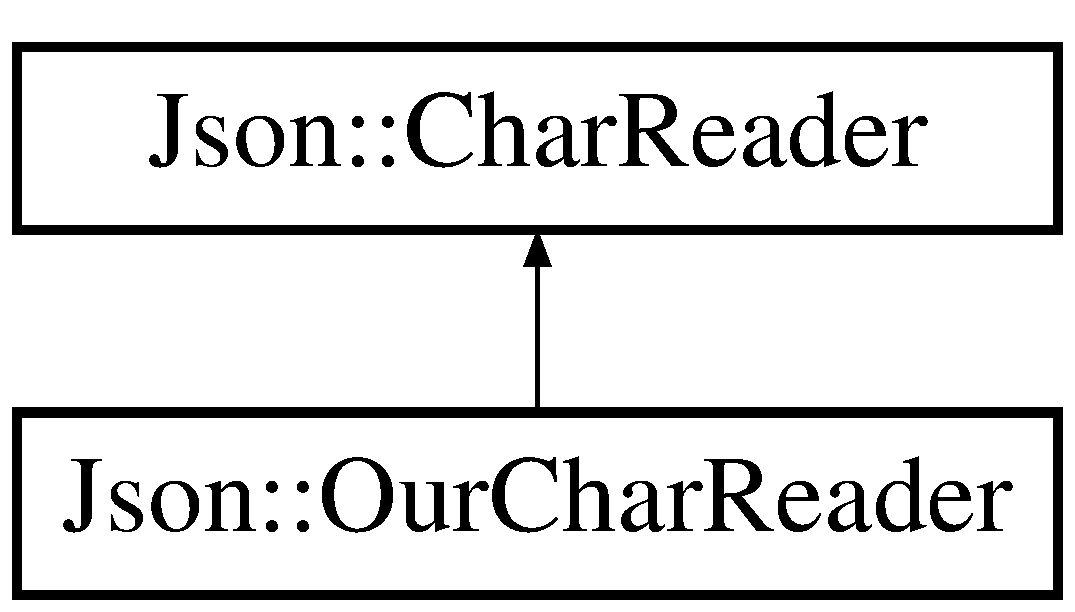
\includegraphics[height=2.000000cm]{class_json_1_1_char_reader}
\end{center}
\end{figure}
\subsection*{Classes}
\begin{DoxyCompactItemize}
\item 
class \hyperlink{class_json_1_1_char_reader_1_1_factory}{Factory}
\end{DoxyCompactItemize}
\subsection*{Public Member Functions}
\begin{DoxyCompactItemize}
\item 
virtual bool \hyperlink{class_json_1_1_char_reader_a48e320be8b13bbc0960cc5808cafec98}{parse} (char const $\ast$begin\+Doc, char const $\ast$end\+Doc, \hyperlink{class_json_1_1_value}{Value} $\ast$root, std\+::string $\ast$errs)=0
\begin{DoxyCompactList}\small\item\em Read a \hyperlink{class_json_1_1_value}{Value} from a \href{http://www.json.org}{\tt J\+S\+O\+N} document. The document must be a U\+T\+F-\/8 encoded string containing the document to read. \end{DoxyCompactList}\end{DoxyCompactItemize}


\subsection{Detailed Description}
Interface for reading J\+S\+O\+N from a char array. 

\subsection{Member Function Documentation}
\hypertarget{class_json_1_1_char_reader_a48e320be8b13bbc0960cc5808cafec98}{}\index{Json\+::\+Char\+Reader@{Json\+::\+Char\+Reader}!parse@{parse}}
\index{parse@{parse}!Json\+::\+Char\+Reader@{Json\+::\+Char\+Reader}}
\subsubsection[{parse}]{\setlength{\rightskip}{0pt plus 5cm}virtual bool Json\+::\+Char\+Reader\+::parse (
\begin{DoxyParamCaption}
\item[{char const $\ast$}]{begin\+Doc, }
\item[{char const $\ast$}]{end\+Doc, }
\item[{{\bf Value} $\ast$}]{root, }
\item[{std\+::string $\ast$}]{errs}
\end{DoxyParamCaption}
)\hspace{0.3cm}{\ttfamily [pure virtual]}}\label{class_json_1_1_char_reader_a48e320be8b13bbc0960cc5808cafec98}


Read a \hyperlink{class_json_1_1_value}{Value} from a \href{http://www.json.org}{\tt J\+S\+O\+N} document. The document must be a U\+T\+F-\/8 encoded string containing the document to read. 


\begin{DoxyParams}{Parameters}
{\em begin\+Doc} & Pointer on the beginning of the U\+T\+F-\/8 encoded string of the document to read. \\
\hline
{\em end\+Doc} & Pointer on the end of the U\+T\+F-\/8 encoded string of the document to read. Must be $>$= begin\+Doc. \\
\hline
{\em root} & \mbox{[}out\mbox{]} Contains the root value of the document if it was successfully parsed. \\
\hline
{\em errs} & \mbox{[}out\mbox{]} Formatted error messages (if not N\+U\+L\+L) a user friendly string that lists errors in the parsed document. \\
\hline
\end{DoxyParams}
\begin{DoxyReturn}{Returns}
{\ttfamily true} if the document was successfully parsed, {\ttfamily false} if an error occurred. 
\end{DoxyReturn}


Implemented in \hyperlink{class_json_1_1_our_char_reader_a52a1fb5fee88d9b63dd462f63b1c9570}{Json\+::\+Our\+Char\+Reader}.



The documentation for this class was generated from the following file\+:\begin{DoxyCompactItemize}
\item 
/home/frank/dev/cpe402/saas/lib/jsoncpp/inc/json.\+h\end{DoxyCompactItemize}

\hypertarget{class_json_1_1_char_reader_builder}{}\section{Json\+:\+:Char\+Reader\+Builder Class Reference}
\label{class_json_1_1_char_reader_builder}\index{Json\+::\+Char\+Reader\+Builder@{Json\+::\+Char\+Reader\+Builder}}


Build a \hyperlink{class_json_1_1_char_reader}{Char\+Reader} implementation.  




{\ttfamily \#include $<$json.\+h$>$}

Inheritance diagram for Json\+:\+:Char\+Reader\+Builder\+:\begin{figure}[H]
\begin{center}
\leavevmode
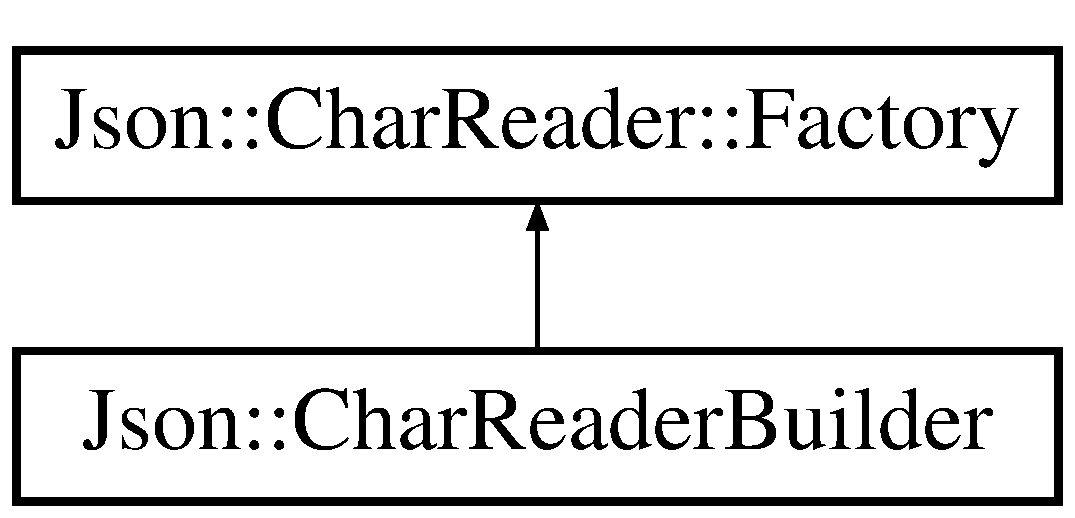
\includegraphics[height=2.000000cm]{class_json_1_1_char_reader_builder}
\end{center}
\end{figure}
\subsection*{Public Member Functions}
\begin{DoxyCompactItemize}
\item 
\hyperlink{class_json_1_1_char_reader}{Char\+Reader} $\ast$ \hyperlink{class_json_1_1_char_reader_builder_a81da7da750111321ff14baf0f0a4c8ae}{new\+Char\+Reader} () const override
\begin{DoxyCompactList}\small\item\em Allocate a \hyperlink{class_json_1_1_char_reader}{Char\+Reader} via operator new(). \end{DoxyCompactList}\item 
bool \hyperlink{class_json_1_1_char_reader_builder_a3d233735a1e4b3c9a2cb9c68f972c02a}{validate} (\hyperlink{class_json_1_1_value}{Json\+::\+Value} $\ast$invalid) const 
\item 
\hyperlink{class_json_1_1_value}{Value} \& \hyperlink{class_json_1_1_char_reader_builder_a324561448113b48eb7aa6e6a5ce3aa0d}{operator\mbox{[}$\,$\mbox{]}} (std\+::string key)
\end{DoxyCompactItemize}
\subsection*{Static Public Member Functions}
\begin{DoxyCompactItemize}
\item 
static void \hyperlink{class_json_1_1_char_reader_builder_a03ff031e06aabff989ab4addc87294ab}{set\+Defaults} (\hyperlink{class_json_1_1_value}{Json\+::\+Value} $\ast$settings)
\item 
static void \hyperlink{class_json_1_1_char_reader_builder_a9c19e3c5475f9072d527810d4bf56749}{strict\+Mode} (\hyperlink{class_json_1_1_value}{Json\+::\+Value} $\ast$settings)
\end{DoxyCompactItemize}
\subsection*{Public Attributes}
\begin{DoxyCompactItemize}
\item 
\hyperlink{class_json_1_1_value}{Json\+::\+Value} \hyperlink{class_json_1_1_char_reader_builder_ac69b7911ad64c171c51ebaf2ea26d958}{settings\+\_\+}
\end{DoxyCompactItemize}


\subsection{Detailed Description}
Build a \hyperlink{class_json_1_1_char_reader}{Char\+Reader} implementation. 

Usage\+: 
\begin{DoxyCode}
\textcolor{keyword}{using namespace }\hyperlink{namespace_json}{Json};
\hyperlink{class_json_1_1_char_reader_builder}{CharReaderBuilder} builder;
builder[\textcolor{stringliteral}{"collectComments"}] = \textcolor{keyword}{false};
\hyperlink{class_json_1_1_value}{Value} value;
std::string errs;
\textcolor{keywordtype}{bool} ok = \hyperlink{namespace_json_acfebeaf759a841173ddce34c4da22486}{parseFromStream}(builder, std::cin, &value, &errs);
\end{DoxyCode}
 

\subsection{Member Function Documentation}
\hypertarget{class_json_1_1_char_reader_builder_a81da7da750111321ff14baf0f0a4c8ae}{}\index{Json\+::\+Char\+Reader\+Builder@{Json\+::\+Char\+Reader\+Builder}!new\+Char\+Reader@{new\+Char\+Reader}}
\index{new\+Char\+Reader@{new\+Char\+Reader}!Json\+::\+Char\+Reader\+Builder@{Json\+::\+Char\+Reader\+Builder}}
\subsubsection[{new\+Char\+Reader}]{\setlength{\rightskip}{0pt plus 5cm}{\bf Char\+Reader} $\ast$ Json\+::\+Char\+Reader\+Builder\+::new\+Char\+Reader (
\begin{DoxyParamCaption}
{}
\end{DoxyParamCaption}
) const\hspace{0.3cm}{\ttfamily [override]}, {\ttfamily [virtual]}}\label{class_json_1_1_char_reader_builder_a81da7da750111321ff14baf0f0a4c8ae}


Allocate a \hyperlink{class_json_1_1_char_reader}{Char\+Reader} via operator new(). 


\begin{DoxyExceptions}{Exceptions}
{\em std\+::exception} & if something goes wrong (e.\+g. invalid settings) \\
\hline
\end{DoxyExceptions}


Implements \hyperlink{class_json_1_1_char_reader_1_1_factory_a4c5862a1ffd432372dbe65cf59de98c4}{Json\+::\+Char\+Reader\+::\+Factory}.

\hypertarget{class_json_1_1_char_reader_builder_a324561448113b48eb7aa6e6a5ce3aa0d}{}\index{Json\+::\+Char\+Reader\+Builder@{Json\+::\+Char\+Reader\+Builder}!operator\mbox{[}$\,$\mbox{]}@{operator[]}}
\index{operator\mbox{[}$\,$\mbox{]}@{operator[]}!Json\+::\+Char\+Reader\+Builder@{Json\+::\+Char\+Reader\+Builder}}
\subsubsection[{operator[]}]{\setlength{\rightskip}{0pt plus 5cm}{\bf Value} \& Json\+::\+Char\+Reader\+Builder\+::operator\mbox{[}$\,$\mbox{]} (
\begin{DoxyParamCaption}
\item[{std\+::string}]{key}
\end{DoxyParamCaption}
)}\label{class_json_1_1_char_reader_builder_a324561448113b48eb7aa6e6a5ce3aa0d}
A simple way to update a specific setting. \hypertarget{class_json_1_1_char_reader_builder_a03ff031e06aabff989ab4addc87294ab}{}\index{Json\+::\+Char\+Reader\+Builder@{Json\+::\+Char\+Reader\+Builder}!set\+Defaults@{set\+Defaults}}
\index{set\+Defaults@{set\+Defaults}!Json\+::\+Char\+Reader\+Builder@{Json\+::\+Char\+Reader\+Builder}}
\subsubsection[{set\+Defaults}]{\setlength{\rightskip}{0pt plus 5cm}void Json\+::\+Char\+Reader\+Builder\+::set\+Defaults (
\begin{DoxyParamCaption}
\item[{{\bf Json\+::\+Value} $\ast$}]{settings}
\end{DoxyParamCaption}
)\hspace{0.3cm}{\ttfamily [static]}}\label{class_json_1_1_char_reader_builder_a03ff031e06aabff989ab4addc87294ab}
Called by ctor, but you can use this to reset settings\+\_\+. \begin{DoxyPrecond}{Precondition}
\textquotesingle{}settings\textquotesingle{} != N\+U\+L\+L (but Json\+::null is fine) 
\end{DoxyPrecond}
\begin{DoxyRemark}{Remarks}
Defaults\+: 
\begin{DoxyCodeInclude}
\end{DoxyCodeInclude}

\end{DoxyRemark}
\mbox{[}Char\+Reader\+Builder\+Defaults\mbox{]}

\mbox{[}Char\+Reader\+Builder\+Defaults\mbox{]} \hypertarget{class_json_1_1_char_reader_builder_a9c19e3c5475f9072d527810d4bf56749}{}\index{Json\+::\+Char\+Reader\+Builder@{Json\+::\+Char\+Reader\+Builder}!strict\+Mode@{strict\+Mode}}
\index{strict\+Mode@{strict\+Mode}!Json\+::\+Char\+Reader\+Builder@{Json\+::\+Char\+Reader\+Builder}}
\subsubsection[{strict\+Mode}]{\setlength{\rightskip}{0pt plus 5cm}void Json\+::\+Char\+Reader\+Builder\+::strict\+Mode (
\begin{DoxyParamCaption}
\item[{{\bf Json\+::\+Value} $\ast$}]{settings}
\end{DoxyParamCaption}
)\hspace{0.3cm}{\ttfamily [static]}}\label{class_json_1_1_char_reader_builder_a9c19e3c5475f9072d527810d4bf56749}
Same as old \hyperlink{class_json_1_1_features_ae23176c14b2e79e81fb61fb1a8ab58ee}{Features\+::strict\+Mode()}. \begin{DoxyPrecond}{Precondition}
\textquotesingle{}settings\textquotesingle{} != N\+U\+L\+L (but Json\+::null is fine) 
\end{DoxyPrecond}
\begin{DoxyRemark}{Remarks}
Defaults\+: 
\begin{DoxyCodeInclude}
\end{DoxyCodeInclude}

\end{DoxyRemark}
\mbox{[}Char\+Reader\+Builder\+Strict\+Mode\mbox{]}

\mbox{[}Char\+Reader\+Builder\+Strict\+Mode\mbox{]} \hypertarget{class_json_1_1_char_reader_builder_a3d233735a1e4b3c9a2cb9c68f972c02a}{}\index{Json\+::\+Char\+Reader\+Builder@{Json\+::\+Char\+Reader\+Builder}!validate@{validate}}
\index{validate@{validate}!Json\+::\+Char\+Reader\+Builder@{Json\+::\+Char\+Reader\+Builder}}
\subsubsection[{validate}]{\setlength{\rightskip}{0pt plus 5cm}bool Json\+::\+Char\+Reader\+Builder\+::validate (
\begin{DoxyParamCaption}
\item[{{\bf Json\+::\+Value} $\ast$}]{invalid}
\end{DoxyParamCaption}
) const}\label{class_json_1_1_char_reader_builder_a3d233735a1e4b3c9a2cb9c68f972c02a}
\begin{DoxyReturn}{Returns}
true if \textquotesingle{}settings\textquotesingle{} are legal and consistent; otherwise, indicate bad settings via \textquotesingle{}invalid\textquotesingle{}. 
\end{DoxyReturn}


\subsection{Member Data Documentation}
\hypertarget{class_json_1_1_char_reader_builder_ac69b7911ad64c171c51ebaf2ea26d958}{}\index{Json\+::\+Char\+Reader\+Builder@{Json\+::\+Char\+Reader\+Builder}!settings\+\_\+@{settings\+\_\+}}
\index{settings\+\_\+@{settings\+\_\+}!Json\+::\+Char\+Reader\+Builder@{Json\+::\+Char\+Reader\+Builder}}
\subsubsection[{settings\+\_\+}]{\setlength{\rightskip}{0pt plus 5cm}{\bf Json\+::\+Value} Json\+::\+Char\+Reader\+Builder\+::settings\+\_\+}\label{class_json_1_1_char_reader_builder_ac69b7911ad64c171c51ebaf2ea26d958}
Configuration of this builder. These are case-\/sensitive. Available settings (case-\/sensitive)\+:
\begin{DoxyItemize}
\item {\ttfamily \char`\"{}collect\+Comments\char`\"{}\+: false or true}
\begin{DoxyItemize}
\item true to collect comment and allow writing them back during serialization, false to discard comments. This parameter is ignored if allow\+Comments is false.
\end{DoxyItemize}
\item {\ttfamily \char`\"{}allow\+Comments\char`\"{}\+: false or true}
\begin{DoxyItemize}
\item true if comments are allowed.
\end{DoxyItemize}
\item {\ttfamily \char`\"{}strict\+Root\char`\"{}\+: false or true}
\begin{DoxyItemize}
\item true if root must be either an array or an object value
\end{DoxyItemize}
\item {\ttfamily \char`\"{}allow\+Dropped\+Null\+Placeholders\char`\"{}\+: false or true}
\begin{DoxyItemize}
\item true if dropped null placeholders are allowed. (See \hyperlink{class_json_1_1_stream_writer_builder}{Stream\+Writer\+Builder}.)
\end{DoxyItemize}
\item {\ttfamily \char`\"{}allow\+Numeric\+Keys\char`\"{}\+: false or true}
\begin{DoxyItemize}
\item true if numeric object keys are allowed.
\end{DoxyItemize}
\item {\ttfamily \char`\"{}allow\+Single\+Quotes\char`\"{}\+: false or true}
\begin{DoxyItemize}
\item true if \textquotesingle{}\textquotesingle{} are allowed for strings (both keys and values)
\end{DoxyItemize}
\item {\ttfamily \char`\"{}stack\+Limit\char`\"{}\+: integer}
\begin{DoxyItemize}
\item Exceeding stack\+Limit (recursive depth of {\ttfamily read\+Value()}) will cause an exception.
\item This is a security issue (seg-\/faults caused by deeply nested J\+S\+O\+N), so the default is low.
\end{DoxyItemize}
\item {\ttfamily \char`\"{}fail\+If\+Extra\char`\"{}\+: false or true}
\begin{DoxyItemize}
\item If true, {\ttfamily parse()} returns false when extra non-\/whitespace trails the J\+S\+O\+N value in the input string.
\end{DoxyItemize}
\item {\ttfamily \char`\"{}reject\+Dup\+Keys\char`\"{}\+: false or true}
\begin{DoxyItemize}
\item If true, {\ttfamily parse()} returns false when a key is duplicated within an object.
\end{DoxyItemize}
\item {\ttfamily \char`\"{}allow\+Special\+Floats\char`\"{}\+: false or true}
\begin{DoxyItemize}
\item If true, special float values (Na\+Ns and infinities) are allowed and their values are lossfree restorable.
\end{DoxyItemize}
\end{DoxyItemize}

You can examine \textquotesingle{}settings\+\_\+` yourself to see the defaults. You can also write and read them just like any J\+S\+O\+N \hyperlink{class_json_1_1_value}{Value}. \begin{DoxySeeAlso}{See also}
\hyperlink{class_json_1_1_char_reader_builder_a03ff031e06aabff989ab4addc87294ab}{set\+Defaults()} 
\end{DoxySeeAlso}


The documentation for this class was generated from the following files\+:\begin{DoxyCompactItemize}
\item 
/home/fpoole/development/cpe406/saas/lib/jsoncpp/inc/json.\+h\item 
/home/fpoole/development/cpe406/saas/lib/jsoncpp/src/jsoncpp.\+cpp\end{DoxyCompactItemize}

\hypertarget{class_client_socket}{}\section{Client\+Socket Class Reference}
\label{class_client_socket}\index{Client\+Socket@{Client\+Socket}}


{\ttfamily \#include $<$Client\+Socket.\+h$>$}

Inheritance diagram for Client\+Socket\+:\begin{figure}[H]
\begin{center}
\leavevmode
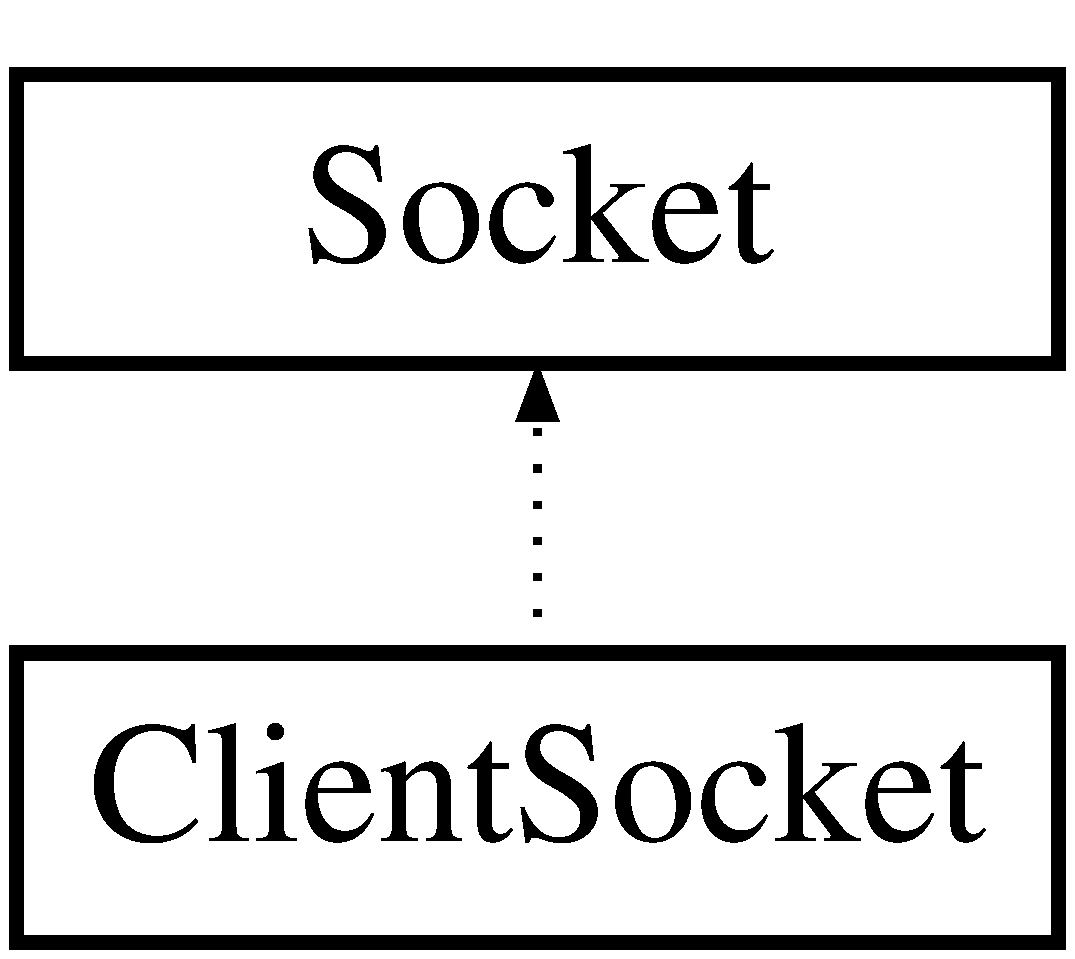
\includegraphics[height=2.000000cm]{class_client_socket}
\end{center}
\end{figure}
\subsection*{Public Member Functions}
\begin{DoxyCompactItemize}
\item 
\hyperlink{class_client_socket_a3e2c121e1538af875d208cb604f0e94c}{Client\+Socket} (std\+::string host, const in\+\_\+port\+\_\+t port)
\item 
virtual \hyperlink{class_client_socket_a9c8af4fc4f56b62ef0ff7d67037f65a3}{$\sim$\+Client\+Socket} ()
\item 
const \hyperlink{class_client_socket}{Client\+Socket} \& \hyperlink{class_client_socket_a2fe5c2037ee6bdcc4d578db1111928ba}{operator$<$$<$} (const std\+::string \&) const 
\item 
const \hyperlink{class_client_socket}{Client\+Socket} \& \hyperlink{class_client_socket_a6cb39e9222b501c8b070de60ef6b5fbc}{operator$>$$>$} (std\+::string \&) const 
\item 
const \hyperlink{class_client_socket}{Client\+Socket} \& \hyperlink{class_client_socket_ac2fbdbdab8ecb0eca85f577ba3b7917b}{operator$<$$<$} (const \+::google\+::protobuf\+::\+Message \&msg) const 
\item 
const \hyperlink{class_client_socket}{Client\+Socket} \& \hyperlink{class_client_socket_a3d8ebe603d979b9bd22ef7bc4d896968}{operator$>$$>$} (\+::google\+::protobuf\+::\+Message \&msg) const 
\end{DoxyCompactItemize}


\subsection{Detailed Description}
A Client \hyperlink{class_socket}{Socket} is a socket that connects to an open port. The client socket should be used when it wants to communicate with an already open socket. String data and protocol buffer data can be sent through the socket 

\subsection{Constructor \& Destructor Documentation}
\hypertarget{class_client_socket_a3e2c121e1538af875d208cb604f0e94c}{}\index{Client\+Socket@{Client\+Socket}!Client\+Socket@{Client\+Socket}}
\index{Client\+Socket@{Client\+Socket}!Client\+Socket@{Client\+Socket}}
\subsubsection[{Client\+Socket}]{\setlength{\rightskip}{0pt plus 5cm}Client\+Socket\+::\+Client\+Socket (
\begin{DoxyParamCaption}
\item[{std\+::string}]{host, }
\item[{const in\+\_\+port\+\_\+t}]{port}
\end{DoxyParamCaption}
)}\label{class_client_socket_a3e2c121e1538af875d208cb604f0e94c}
Create a new socket, and connect to the specified host and port. 
\begin{DoxyParams}{Parameters}
{\em host} & the address or address alias of the host computer \\
\hline
{\em port} & the port to connect to \\
\hline
\end{DoxyParams}
\hypertarget{class_client_socket_a9c8af4fc4f56b62ef0ff7d67037f65a3}{}\index{Client\+Socket@{Client\+Socket}!````~Client\+Socket@{$\sim$\+Client\+Socket}}
\index{````~Client\+Socket@{$\sim$\+Client\+Socket}!Client\+Socket@{Client\+Socket}}
\subsubsection[{$\sim$\+Client\+Socket}]{\setlength{\rightskip}{0pt plus 5cm}virtual Client\+Socket\+::$\sim$\+Client\+Socket (
\begin{DoxyParamCaption}
{}
\end{DoxyParamCaption}
)\hspace{0.3cm}{\ttfamily [inline]}, {\ttfamily [virtual]}}\label{class_client_socket_a9c8af4fc4f56b62ef0ff7d67037f65a3}
Close the socket. 

\subsection{Member Function Documentation}
\hypertarget{class_client_socket_a2fe5c2037ee6bdcc4d578db1111928ba}{}\index{Client\+Socket@{Client\+Socket}!operator$<$$<$@{operator$<$$<$}}
\index{operator$<$$<$@{operator$<$$<$}!Client\+Socket@{Client\+Socket}}
\subsubsection[{operator$<$$<$}]{\setlength{\rightskip}{0pt plus 5cm}const {\bf Client\+Socket} \& Client\+Socket\+::operator$<$$<$ (
\begin{DoxyParamCaption}
\item[{const std\+::string \&}]{s}
\end{DoxyParamCaption}
) const}\label{class_client_socket_a2fe5c2037ee6bdcc4d578db1111928ba}
Send string data to the connected host. 
\begin{DoxyParams}{Parameters}
{\em string} & the data to send \\
\hline
\end{DoxyParams}
\begin{DoxyReturn}{Returns}
the socket, for chaining 
\end{DoxyReturn}
\hypertarget{class_client_socket_ac2fbdbdab8ecb0eca85f577ba3b7917b}{}\index{Client\+Socket@{Client\+Socket}!operator$<$$<$@{operator$<$$<$}}
\index{operator$<$$<$@{operator$<$$<$}!Client\+Socket@{Client\+Socket}}
\subsubsection[{operator$<$$<$}]{\setlength{\rightskip}{0pt plus 5cm}const {\bf Client\+Socket} \& Client\+Socket\+::operator$<$$<$ (
\begin{DoxyParamCaption}
\item[{const \+::google\+::protobuf\+::\+Message \&}]{msg}
\end{DoxyParamCaption}
) const}\label{class_client_socket_ac2fbdbdab8ecb0eca85f577ba3b7917b}
Send protocol buffer data from the connected host. 
\begin{DoxyParams}{Parameters}
{\em msg} & the message to send \\
\hline
\end{DoxyParams}
\begin{DoxyReturn}{Returns}
the \hyperlink{class_socket}{Socket}, for chaining 
\end{DoxyReturn}
\hypertarget{class_client_socket_a6cb39e9222b501c8b070de60ef6b5fbc}{}\index{Client\+Socket@{Client\+Socket}!operator$>$$>$@{operator$>$$>$}}
\index{operator$>$$>$@{operator$>$$>$}!Client\+Socket@{Client\+Socket}}
\subsubsection[{operator$>$$>$}]{\setlength{\rightskip}{0pt plus 5cm}const {\bf Client\+Socket} \& Client\+Socket\+::operator$>$$>$ (
\begin{DoxyParamCaption}
\item[{std\+::string \&}]{s}
\end{DoxyParamCaption}
) const}\label{class_client_socket_a6cb39e9222b501c8b070de60ef6b5fbc}
Receive string data from the connected host. 
\begin{DoxyParams}{Parameters}
{\em string} & the string to read data into \\
\hline
\end{DoxyParams}
\begin{DoxyReturn}{Returns}
the socket, for chaining 
\end{DoxyReturn}
\hypertarget{class_client_socket_a3d8ebe603d979b9bd22ef7bc4d896968}{}\index{Client\+Socket@{Client\+Socket}!operator$>$$>$@{operator$>$$>$}}
\index{operator$>$$>$@{operator$>$$>$}!Client\+Socket@{Client\+Socket}}
\subsubsection[{operator$>$$>$}]{\setlength{\rightskip}{0pt plus 5cm}const {\bf Client\+Socket} \& Client\+Socket\+::operator$>$$>$ (
\begin{DoxyParamCaption}
\item[{\+::google\+::protobuf\+::\+Message \&}]{msg}
\end{DoxyParamCaption}
) const}\label{class_client_socket_a3d8ebe603d979b9bd22ef7bc4d896968}
Receive protocol buffer data from the connected host. 
\begin{DoxyParams}{Parameters}
{\em msg} & the message to read into \\
\hline
\end{DoxyParams}
\begin{DoxyReturn}{Returns}
the socket, for chaining 
\end{DoxyReturn}


The documentation for this class was generated from the following files\+:\begin{DoxyCompactItemize}
\item 
/home/fpoole/development/cpe406/saas/lib/network/inc/Client\+Socket.\+h\item 
/home/fpoole/development/cpe406/saas/lib/network/src/Client\+Socket.\+cpp\end{DoxyCompactItemize}

\input{struct_cluster}
\hypertarget{struct_json_1_1_comment_style}{}\section{Json\+:\+:Comment\+Style Struct Reference}
\label{struct_json_1_1_comment_style}\index{Json\+::\+Comment\+Style@{Json\+::\+Comment\+Style}}


Scoped enums are not available until C++11.  


\subsection*{Public Types}
\begin{DoxyCompactItemize}
\item 
enum \hyperlink{struct_json_1_1_comment_style_a51fc08f3518fd81eba12f340d19a3d0c}{Enum} \{ \hyperlink{struct_json_1_1_comment_style_a51fc08f3518fd81eba12f340d19a3d0cac8b32a8bae63414c8647d4919da8d437}{None}, 
\hyperlink{struct_json_1_1_comment_style_a51fc08f3518fd81eba12f340d19a3d0cac65238f050773c107690a456e9c05c98}{Most}, 
\hyperlink{struct_json_1_1_comment_style_a51fc08f3518fd81eba12f340d19a3d0ca32302c0b97190c1808b3e38f367fef01}{All}
 \}\begin{DoxyCompactList}\small\item\em Decide whether to write comments. \end{DoxyCompactList}
\end{DoxyCompactItemize}


\subsection{Detailed Description}
Scoped enums are not available until C++11. 

\subsection{Member Enumeration Documentation}
\index{Json\+::\+Comment\+Style@{Json\+::\+Comment\+Style}!Enum@{Enum}}
\index{Enum@{Enum}!Json\+::\+Comment\+Style@{Json\+::\+Comment\+Style}}
\subsubsection[{\texorpdfstring{Enum}{Enum}}]{\setlength{\rightskip}{0pt plus 5cm}enum {\bf Json\+::\+Comment\+Style\+::\+Enum}}\hypertarget{struct_json_1_1_comment_style_a51fc08f3518fd81eba12f340d19a3d0c}{}\label{struct_json_1_1_comment_style_a51fc08f3518fd81eba12f340d19a3d0c}


Decide whether to write comments. 

\begin{Desc}
\item[Enumerator]\par
\begin{description}
\index{None@{None}!Json\+::\+Comment\+Style@{Json\+::\+Comment\+Style}}\index{Json\+::\+Comment\+Style@{Json\+::\+Comment\+Style}!None@{None}}\item[{\em 
None\hypertarget{struct_json_1_1_comment_style_a51fc08f3518fd81eba12f340d19a3d0cac8b32a8bae63414c8647d4919da8d437}{}\label{struct_json_1_1_comment_style_a51fc08f3518fd81eba12f340d19a3d0cac8b32a8bae63414c8647d4919da8d437}
}]Drop all comments. \index{Most@{Most}!Json\+::\+Comment\+Style@{Json\+::\+Comment\+Style}}\index{Json\+::\+Comment\+Style@{Json\+::\+Comment\+Style}!Most@{Most}}\item[{\em 
Most\hypertarget{struct_json_1_1_comment_style_a51fc08f3518fd81eba12f340d19a3d0cac65238f050773c107690a456e9c05c98}{}\label{struct_json_1_1_comment_style_a51fc08f3518fd81eba12f340d19a3d0cac65238f050773c107690a456e9c05c98}
}]Recover odd behavior of previous versions (not implemented yet). \index{All@{All}!Json\+::\+Comment\+Style@{Json\+::\+Comment\+Style}}\index{Json\+::\+Comment\+Style@{Json\+::\+Comment\+Style}!All@{All}}\item[{\em 
All\hypertarget{struct_json_1_1_comment_style_a51fc08f3518fd81eba12f340d19a3d0ca32302c0b97190c1808b3e38f367fef01}{}\label{struct_json_1_1_comment_style_a51fc08f3518fd81eba12f340d19a3d0ca32302c0b97190c1808b3e38f367fef01}
}]Keep all comments. \end{description}
\end{Desc}


The documentation for this struct was generated from the following file\+:\begin{DoxyCompactItemize}
\item 
/\+Users/\+Dat/\+Clion\+Projects/saas/lib/jsoncpp/src/jsoncpp.\+cpp\end{DoxyCompactItemize}

\hypertarget{class_silent_orbit_1_1_protocol_buffers_1_1_concurrent_bag_stack}{}\section{Silent\+Orbit.\+Protocol\+Buffers.\+Concurrent\+Bag\+Stack Class Reference}
\label{class_silent_orbit_1_1_protocol_buffers_1_1_concurrent_bag_stack}\index{Silent\+Orbit.\+Protocol\+Buffers.\+Concurrent\+Bag\+Stack@{Silent\+Orbit.\+Protocol\+Buffers.\+Concurrent\+Bag\+Stack}}
Inheritance diagram for Silent\+Orbit.\+Protocol\+Buffers.\+Concurrent\+Bag\+Stack\+:\begin{figure}[H]
\begin{center}
\leavevmode
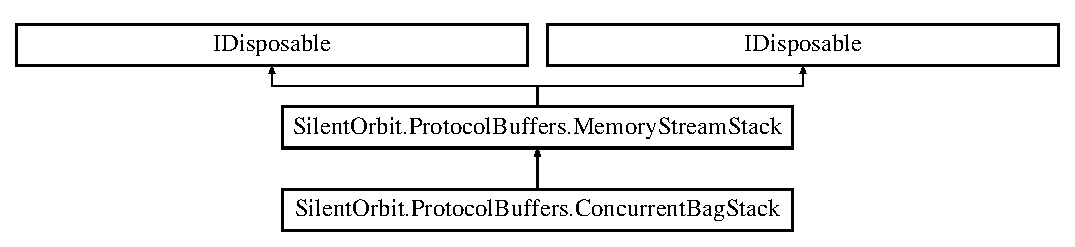
\includegraphics[height=2.876712cm]{class_silent_orbit_1_1_protocol_buffers_1_1_concurrent_bag_stack}
\end{center}
\end{figure}
\subsection*{Public Member Functions}
\begin{DoxyCompactItemize}
\item 
Memory\+Stream \hyperlink{class_silent_orbit_1_1_protocol_buffers_1_1_concurrent_bag_stack_adb6ba4bd478a1e11e135cbbe7676ce1d}{Pop} ()
\begin{DoxyCompactList}\small\item\em The returned stream is not reset. You must call .Set\+Length(0) before using it. This is done in the generated code. \end{DoxyCompactList}\item 
void {\bfseries Push} (Memory\+Stream stream)\hypertarget{class_silent_orbit_1_1_protocol_buffers_1_1_concurrent_bag_stack_ab262efbb9db8f09224f12ef1e98731df}{}\label{class_silent_orbit_1_1_protocol_buffers_1_1_concurrent_bag_stack_ab262efbb9db8f09224f12ef1e98731df}

\item 
void {\bfseries Dispose} ()\hypertarget{class_silent_orbit_1_1_protocol_buffers_1_1_concurrent_bag_stack_aa386d53d821088a236e688f8205b05f8}{}\label{class_silent_orbit_1_1_protocol_buffers_1_1_concurrent_bag_stack_aa386d53d821088a236e688f8205b05f8}

\end{DoxyCompactItemize}


\subsection{Member Function Documentation}
\index{Silent\+Orbit\+::\+Protocol\+Buffers\+::\+Concurrent\+Bag\+Stack@{Silent\+Orbit\+::\+Protocol\+Buffers\+::\+Concurrent\+Bag\+Stack}!Pop@{Pop}}
\index{Pop@{Pop}!Silent\+Orbit\+::\+Protocol\+Buffers\+::\+Concurrent\+Bag\+Stack@{Silent\+Orbit\+::\+Protocol\+Buffers\+::\+Concurrent\+Bag\+Stack}}
\subsubsection[{\texorpdfstring{Pop()}{Pop()}}]{\setlength{\rightskip}{0pt plus 5cm}Memory\+Stream Silent\+Orbit.\+Protocol\+Buffers.\+Concurrent\+Bag\+Stack.\+Pop (
\begin{DoxyParamCaption}
{}
\end{DoxyParamCaption}
)\hspace{0.3cm}{\ttfamily [inline]}}\hypertarget{class_silent_orbit_1_1_protocol_buffers_1_1_concurrent_bag_stack_adb6ba4bd478a1e11e135cbbe7676ce1d}{}\label{class_silent_orbit_1_1_protocol_buffers_1_1_concurrent_bag_stack_adb6ba4bd478a1e11e135cbbe7676ce1d}


The returned stream is not reset. You must call .Set\+Length(0) before using it. This is done in the generated code. 



Implements \hyperlink{interface_silent_orbit_1_1_protocol_buffers_1_1_memory_stream_stack}{Silent\+Orbit.\+Protocol\+Buffers.\+Memory\+Stream\+Stack}.



The documentation for this class was generated from the following file\+:\begin{DoxyCompactItemize}
\item 
/home/andrea/\+Clion\+Projects/saas/cdti/\+Protobuf\+Tcas\+Demo/\+Protobuf\+Tcas\+Demo/Protocol\+Parser.\+cs\end{DoxyCompactItemize}

\input{struct_correlation_aircraft}
\hypertarget{class_example_script}{}\section{Example\+Script Class Reference}
\label{class_example_script}\index{Example\+Script@{Example\+Script}}
Inheritance diagram for Example\+Script\+:\begin{figure}[H]
\begin{center}
\leavevmode
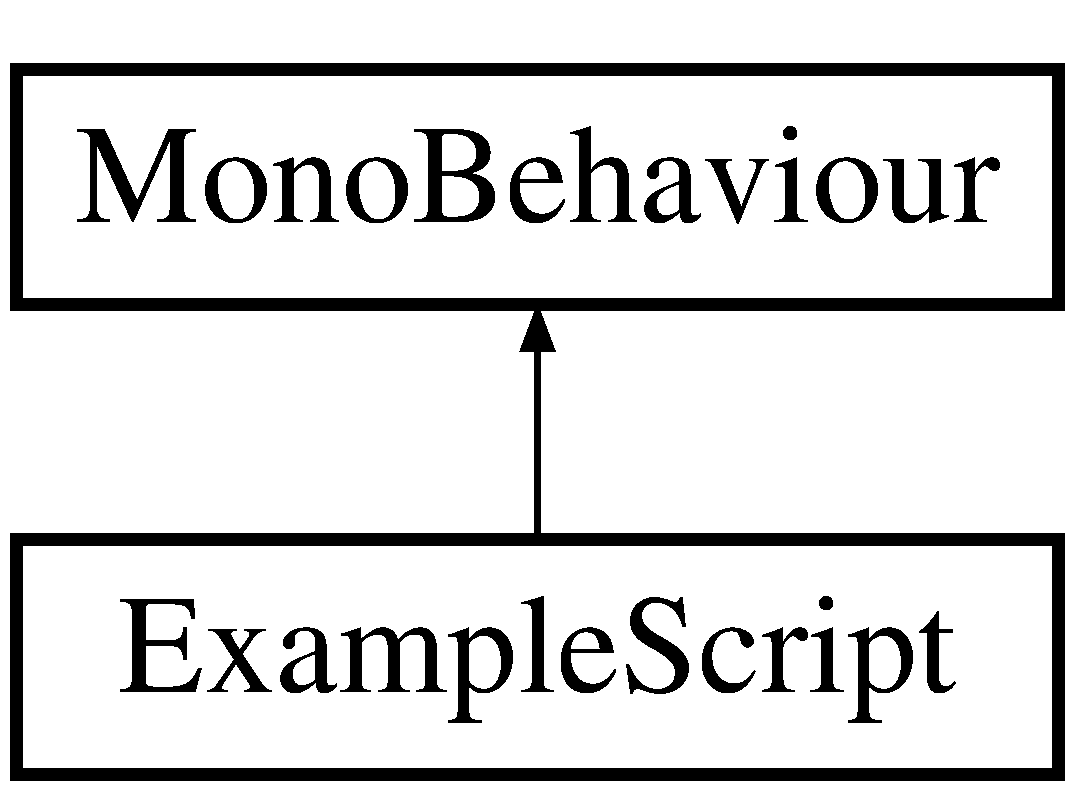
\includegraphics[height=2.000000cm]{class_example_script}
\end{center}
\end{figure}


The documentation for this class was generated from the following file\+:\begin{DoxyCompactItemize}
\item 
/home/frank/dev/cpe402/saas/cdti/\+C\+D\+T\+I\+Unity/\+Assets/\+Ciela\+Spike/\+Thread Ninja/\+Example/Example\+Script.\+cs\end{DoxyCompactItemize}

\hypertarget{class_json_1_1_exception}{}\section{Json\+:\+:Exception Class Reference}
\label{class_json_1_1_exception}\index{Json\+::\+Exception@{Json\+::\+Exception}}


{\ttfamily \#include $<$json.\+h$>$}

Inheritance diagram for Json\+:\+:Exception\+:\begin{figure}[H]
\begin{center}
\leavevmode
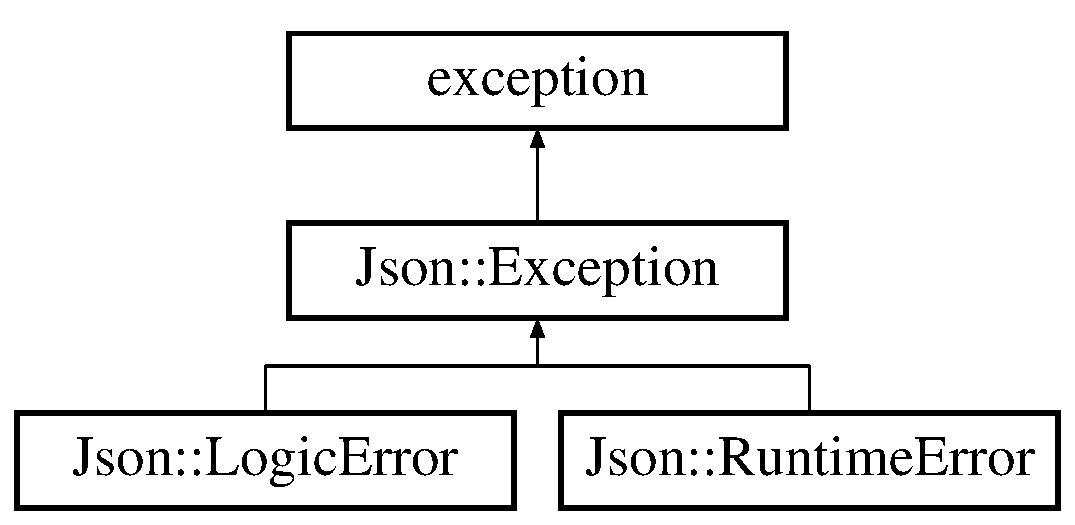
\includegraphics[height=3.000000cm]{class_json_1_1_exception}
\end{center}
\end{figure}
\subsection*{Public Member Functions}
\begin{DoxyCompactItemize}
\item 
\hypertarget{class_json_1_1_exception_a7a974afaa4993e796ec0c118bc4296cf}{}{\bfseries Exception} (std\+::string const \&msg)\label{class_json_1_1_exception_a7a974afaa4993e796ec0c118bc4296cf}

\item 
\hypertarget{class_json_1_1_exception_aa1c30265e0d091a33b1b52d9a815f3e5}{}char const $\ast$ {\bfseries what} () const override  throw ()\label{class_json_1_1_exception_aa1c30265e0d091a33b1b52d9a815f3e5}

\end{DoxyCompactItemize}
\subsection*{Protected Attributes}
\begin{DoxyCompactItemize}
\item 
\hypertarget{class_json_1_1_exception_a26b7dfcd51256ad4da2742bbd0e14a24}{}std\+::string {\bfseries msg\+\_\+}\label{class_json_1_1_exception_a26b7dfcd51256ad4da2742bbd0e14a24}

\end{DoxyCompactItemize}


\subsection{Detailed Description}
Base class for all exceptions we throw.

We use nothing but these internally. Of course, S\+T\+L can throw others. 

The documentation for this class was generated from the following files\+:\begin{DoxyCompactItemize}
\item 
/home/frank/dev/cpe402/saas/lib/jsoncpp/inc/json.\+h\item 
/home/frank/dev/cpe402/saas/lib/jsoncpp/src/jsoncpp.\+cpp\end{DoxyCompactItemize}

\hypertarget{class_json_1_1_char_reader_1_1_factory}{}\section{Json\+:\+:Char\+Reader\+:\+:Factory Class Reference}
\label{class_json_1_1_char_reader_1_1_factory}\index{Json\+::\+Char\+Reader\+::\+Factory@{Json\+::\+Char\+Reader\+::\+Factory}}
Inheritance diagram for Json\+:\+:Char\+Reader\+:\+:Factory\+:\begin{figure}[H]
\begin{center}
\leavevmode
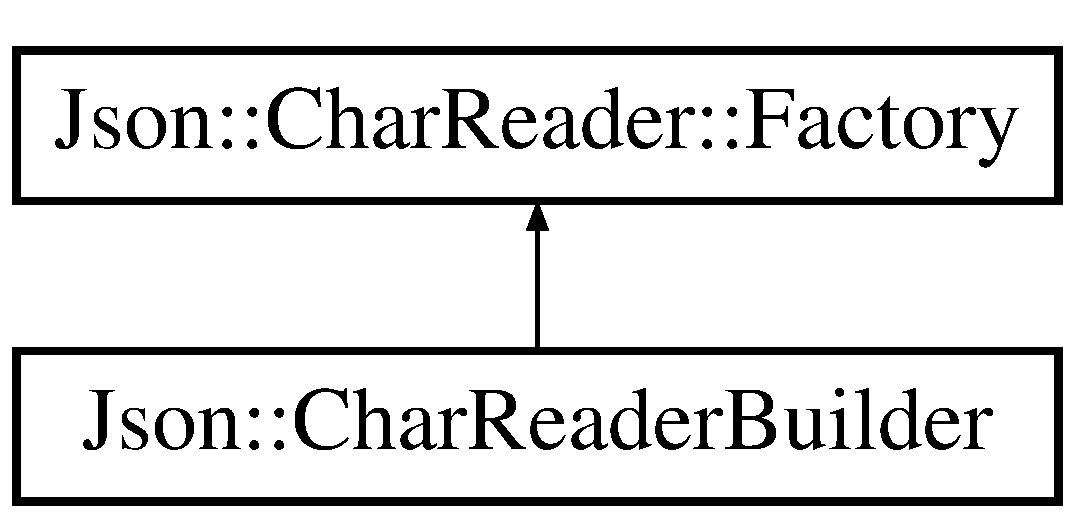
\includegraphics[height=2.000000cm]{class_json_1_1_char_reader_1_1_factory}
\end{center}
\end{figure}
\subsection*{Public Member Functions}
\begin{DoxyCompactItemize}
\item 
virtual \hyperlink{class_json_1_1_char_reader}{Char\+Reader} $\ast$ \hyperlink{class_json_1_1_char_reader_1_1_factory_a497112c51f36a676aeb496c3a91d38d0}{new\+Char\+Reader} () const  =0
\begin{DoxyCompactList}\small\item\em Allocate a \hyperlink{class_json_1_1_char_reader}{Char\+Reader} via operator new(). \end{DoxyCompactList}\end{DoxyCompactItemize}


\subsection{Member Function Documentation}
\index{Json\+::\+Char\+Reader\+::\+Factory@{Json\+::\+Char\+Reader\+::\+Factory}!new\+Char\+Reader@{new\+Char\+Reader}}
\index{new\+Char\+Reader@{new\+Char\+Reader}!Json\+::\+Char\+Reader\+::\+Factory@{Json\+::\+Char\+Reader\+::\+Factory}}
\subsubsection[{\texorpdfstring{new\+Char\+Reader() const  =0}{newCharReader() const  =0}}]{\setlength{\rightskip}{0pt plus 5cm}virtual {\bf Char\+Reader}$\ast$ Json\+::\+Char\+Reader\+::\+Factory\+::new\+Char\+Reader (
\begin{DoxyParamCaption}
{}
\end{DoxyParamCaption}
) const\hspace{0.3cm}{\ttfamily [pure virtual]}}\hypertarget{class_json_1_1_char_reader_1_1_factory_a497112c51f36a676aeb496c3a91d38d0}{}\label{class_json_1_1_char_reader_1_1_factory_a497112c51f36a676aeb496c3a91d38d0}


Allocate a \hyperlink{class_json_1_1_char_reader}{Char\+Reader} via operator new(). 


\begin{DoxyExceptions}{Exceptions}
{\em std\+::exception} & if something goes wrong (e.\+g. invalid settings) \\
\hline
\end{DoxyExceptions}


Implemented in \hyperlink{class_json_1_1_char_reader_builder_a29e41475c2b40a9ab3da10e7c09f6bfd}{Json\+::\+Char\+Reader\+Builder}.



The documentation for this class was generated from the following file\+:\begin{DoxyCompactItemize}
\item 
/home/andrea/\+Clion\+Projects/saas/lib/jsoncpp/inc/json.\+h\end{DoxyCompactItemize}

\hypertarget{class_json_1_1_stream_writer_1_1_factory}{}\section{Json\+:\+:Stream\+Writer\+:\+:Factory Class Reference}
\label{class_json_1_1_stream_writer_1_1_factory}\index{Json\+::\+Stream\+Writer\+::\+Factory@{Json\+::\+Stream\+Writer\+::\+Factory}}


A simple abstract factory.  




{\ttfamily \#include $<$json.\+h$>$}

Inheritance diagram for Json\+:\+:Stream\+Writer\+:\+:Factory\+:\begin{figure}[H]
\begin{center}
\leavevmode
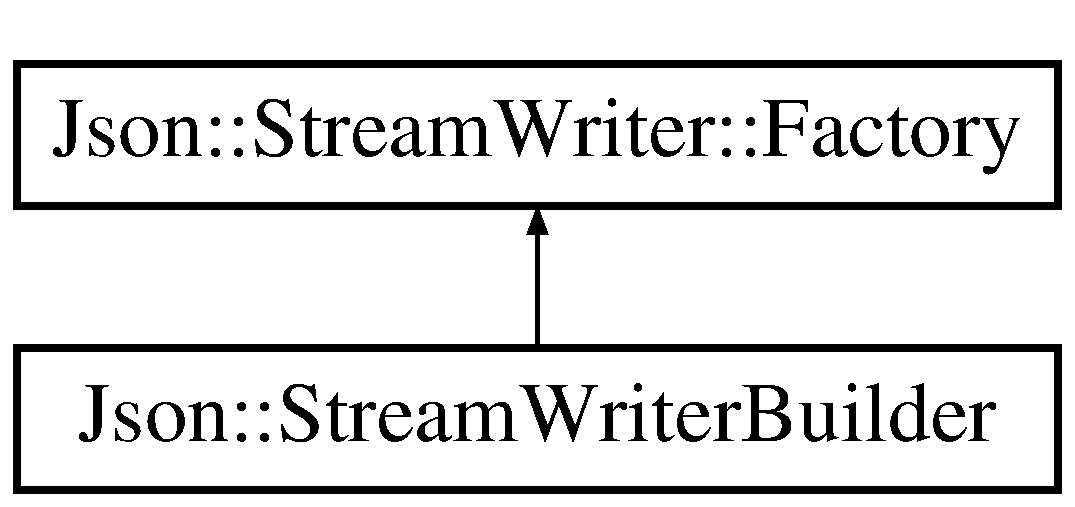
\includegraphics[height=2.000000cm]{class_json_1_1_stream_writer_1_1_factory}
\end{center}
\end{figure}
\subsection*{Public Member Functions}
\begin{DoxyCompactItemize}
\item 
virtual \hyperlink{class_json_1_1_stream_writer}{Stream\+Writer} $\ast$ \hyperlink{class_json_1_1_stream_writer_1_1_factory_a9d30ec53e8288cd53befccf1009c5f31}{new\+Stream\+Writer} () const =0
\begin{DoxyCompactList}\small\item\em Allocate a \hyperlink{class_json_1_1_char_reader}{Char\+Reader} via operator new(). \end{DoxyCompactList}\end{DoxyCompactItemize}


\subsection{Detailed Description}
A simple abstract factory. 

\subsection{Member Function Documentation}
\hypertarget{class_json_1_1_stream_writer_1_1_factory_a9d30ec53e8288cd53befccf1009c5f31}{}\index{Json\+::\+Stream\+Writer\+::\+Factory@{Json\+::\+Stream\+Writer\+::\+Factory}!new\+Stream\+Writer@{new\+Stream\+Writer}}
\index{new\+Stream\+Writer@{new\+Stream\+Writer}!Json\+::\+Stream\+Writer\+::\+Factory@{Json\+::\+Stream\+Writer\+::\+Factory}}
\subsubsection[{new\+Stream\+Writer}]{\setlength{\rightskip}{0pt plus 5cm}virtual {\bf Stream\+Writer}$\ast$ Json\+::\+Stream\+Writer\+::\+Factory\+::new\+Stream\+Writer (
\begin{DoxyParamCaption}
{}
\end{DoxyParamCaption}
) const\hspace{0.3cm}{\ttfamily [pure virtual]}}\label{class_json_1_1_stream_writer_1_1_factory_a9d30ec53e8288cd53befccf1009c5f31}


Allocate a \hyperlink{class_json_1_1_char_reader}{Char\+Reader} via operator new(). 


\begin{DoxyExceptions}{Exceptions}
{\em std\+::exception} & if something goes wrong (e.\+g. invalid settings) \\
\hline
\end{DoxyExceptions}


Implemented in \hyperlink{class_json_1_1_stream_writer_builder_a042d21b84d8c5bede52a764e2ada7d65}{Json\+::\+Stream\+Writer\+Builder}.



The documentation for this class was generated from the following files\+:\begin{DoxyCompactItemize}
\item 
/home/fpoole/development/cpe406/saas/lib/jsoncpp/inc/json.\+h\item 
/home/fpoole/development/cpe406/saas/lib/jsoncpp/src/jsoncpp.\+cpp\end{DoxyCompactItemize}

\hypertarget{class_json_1_1_fast_writer}{}\section{Json\+:\+:Fast\+Writer Class Reference}
\label{class_json_1_1_fast_writer}\index{Json\+::\+Fast\+Writer@{Json\+::\+Fast\+Writer}}


Outputs a \hyperlink{class_json_1_1_value}{Value} in \href{http://www.json.org}{\tt J\+S\+ON} format without formatting (not human friendly).  




{\ttfamily \#include $<$json.\+h$>$}

Inheritance diagram for Json\+:\+:Fast\+Writer\+:\begin{figure}[H]
\begin{center}
\leavevmode
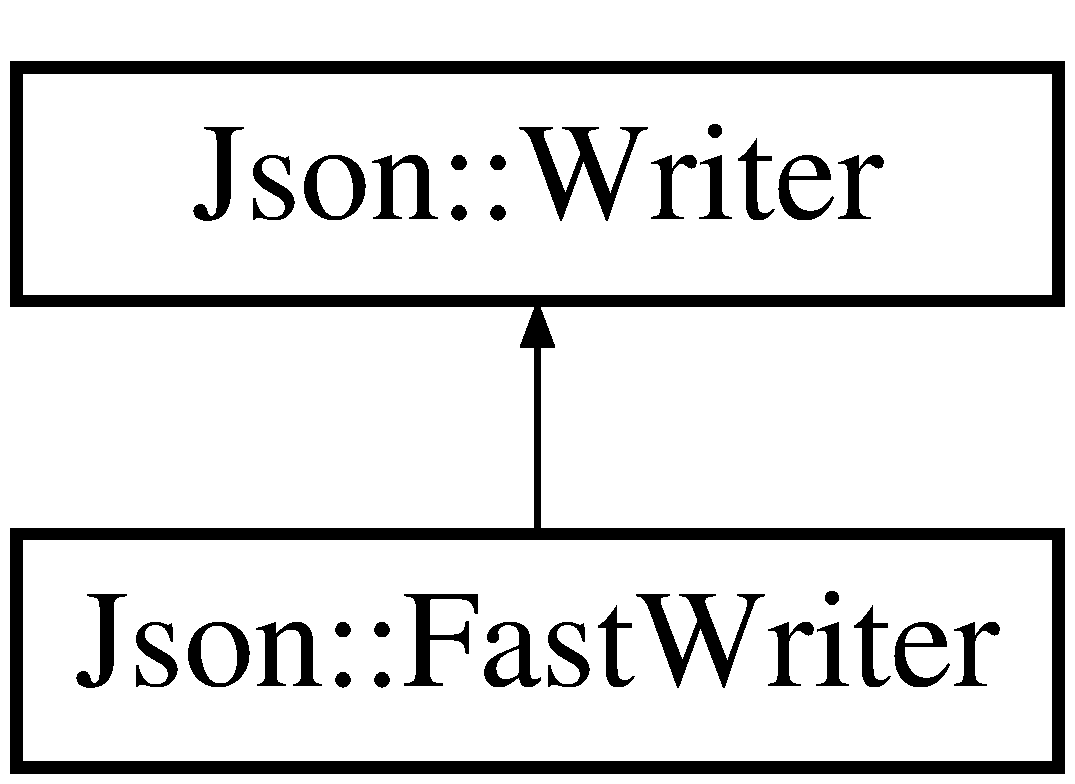
\includegraphics[height=2.000000cm]{class_json_1_1_fast_writer}
\end{center}
\end{figure}
\subsection*{Public Member Functions}
\begin{DoxyCompactItemize}
\item 
void {\bfseries enable\+Y\+A\+M\+L\+Compatibility} ()\hypertarget{class_json_1_1_fast_writer_a78d98e9f76d33660ad6e6a1abe287d45}{}\label{class_json_1_1_fast_writer_a78d98e9f76d33660ad6e6a1abe287d45}

\item 
void \hyperlink{class_json_1_1_fast_writer_a6e93d8dce951e408517311026a065b40}{drop\+Null\+Placeholders} ()\hypertarget{class_json_1_1_fast_writer_a6e93d8dce951e408517311026a065b40}{}\label{class_json_1_1_fast_writer_a6e93d8dce951e408517311026a065b40}

\begin{DoxyCompactList}\small\item\em Drop the \char`\"{}null\char`\"{} string from the writer\textquotesingle{}s output for null\+Values. Strictly speaking, this is not valid J\+S\+ON. But when the output is being fed to a browser\textquotesingle{}s Javascript, it makes for smaller output and the browser can handle the output just fine. \end{DoxyCompactList}\item 
void {\bfseries omit\+Ending\+Line\+Feed} ()\hypertarget{class_json_1_1_fast_writer_af4ee077d365d75941fb2688d97207a55}{}\label{class_json_1_1_fast_writer_af4ee077d365d75941fb2688d97207a55}

\item 
std\+::string {\bfseries write} (const \hyperlink{class_json_1_1_value}{Value} \&root) override\hypertarget{class_json_1_1_fast_writer_aee69e3f778982ec9218c1a5a7c6a3e7a}{}\label{class_json_1_1_fast_writer_aee69e3f778982ec9218c1a5a7c6a3e7a}

\end{DoxyCompactItemize}


\subsection{Detailed Description}
Outputs a \hyperlink{class_json_1_1_value}{Value} in \href{http://www.json.org}{\tt J\+S\+ON} format without formatting (not human friendly). 

The J\+S\+ON document is written in a single line. It is not intended for \textquotesingle{}human\textquotesingle{} consumption, but may be usefull to support feature such as R\+PC where bandwith is limited. \begin{DoxySeeAlso}{See also}
\hyperlink{class_json_1_1_reader}{Reader}, \hyperlink{class_json_1_1_value}{Value} 
\end{DoxySeeAlso}
\begin{DoxyRefDesc}{Deprecated}
\item[\hyperlink{deprecated__deprecated000008}{Deprecated}]Use \hyperlink{class_json_1_1_stream_writer_builder}{Stream\+Writer\+Builder}. \end{DoxyRefDesc}


The documentation for this class was generated from the following files\+:\begin{DoxyCompactItemize}
\item 
/\+Users/\+Dat/\+Clion\+Projects/saas/lib/jsoncpp/inc/json.\+h\item 
/\+Users/\+Dat/\+Clion\+Projects/saas/lib/jsoncpp/src/jsoncpp.\+cpp\end{DoxyCompactItemize}

\hypertarget{class_json_1_1_features}{}\section{Json\+:\+:Features Class Reference}
\label{class_json_1_1_features}\index{Json\+::\+Features@{Json\+::\+Features}}


Configuration passed to reader and writer. This configuration object can be used to force the \hyperlink{class_json_1_1_reader}{Reader} or \hyperlink{class_json_1_1_writer}{Writer} to behave in a standard conforming way.  




{\ttfamily \#include $<$json.\+h$>$}

\subsection*{Public Member Functions}
\begin{DoxyCompactItemize}
\item 
\hypertarget{class_json_1_1_features_ad15a091cb61bb31323299a95970d2644}{}\hyperlink{class_json_1_1_features_ad15a091cb61bb31323299a95970d2644}{Features} ()\label{class_json_1_1_features_ad15a091cb61bb31323299a95970d2644}

\begin{DoxyCompactList}\small\item\em Initialize the configuration like Json\+Config\+::all\+Features;. \end{DoxyCompactList}\end{DoxyCompactItemize}
\subsection*{Static Public Member Functions}
\begin{DoxyCompactItemize}
\item 
static \hyperlink{class_json_1_1_features}{Features} \hyperlink{class_json_1_1_features_a63894da6e2c100b38741fa933f3d33ae}{all} ()
\begin{DoxyCompactList}\small\item\em A configuration that allows all features and assumes all strings are U\+T\+F-\/8. \end{DoxyCompactList}\item 
static \hyperlink{class_json_1_1_features}{Features} \hyperlink{class_json_1_1_features_ae23176c14b2e79e81fb61fb1a8ab58ee}{strict\+Mode} ()
\begin{DoxyCompactList}\small\item\em A configuration that is strictly compatible with the J\+S\+O\+N specification. \end{DoxyCompactList}\end{DoxyCompactItemize}
\subsection*{Public Attributes}
\begin{DoxyCompactItemize}
\item 
\hypertarget{class_json_1_1_features_a33afd389719624b6bdb23950b3c346c9}{}bool \hyperlink{class_json_1_1_features_a33afd389719624b6bdb23950b3c346c9}{allow\+Comments\+\_\+}\label{class_json_1_1_features_a33afd389719624b6bdb23950b3c346c9}

\begin{DoxyCompactList}\small\item\em {\ttfamily true} if comments are allowed. Default\+: {\ttfamily true}. \end{DoxyCompactList}\item 
bool \hyperlink{class_json_1_1_features_a1162c37a1458adc32582b585b552f9c3}{strict\+Root\+\_\+}
\item 
\hypertarget{class_json_1_1_features_a5076aa72c05c7596ac339ede36c97a6a}{}bool \hyperlink{class_json_1_1_features_a5076aa72c05c7596ac339ede36c97a6a}{allow\+Dropped\+Null\+Placeholders\+\_\+}\label{class_json_1_1_features_a5076aa72c05c7596ac339ede36c97a6a}

\begin{DoxyCompactList}\small\item\em {\ttfamily true} if dropped null placeholders are allowed. Default\+: {\ttfamily false}. \end{DoxyCompactList}\item 
\hypertarget{class_json_1_1_features_aff3cb16b79d15d3d761b11a0dd6d4d6b}{}bool \hyperlink{class_json_1_1_features_aff3cb16b79d15d3d761b11a0dd6d4d6b}{allow\+Numeric\+Keys\+\_\+}\label{class_json_1_1_features_aff3cb16b79d15d3d761b11a0dd6d4d6b}

\begin{DoxyCompactList}\small\item\em {\ttfamily true} if numeric object key are allowed. Default\+: {\ttfamily false}. \end{DoxyCompactList}\end{DoxyCompactItemize}


\subsection{Detailed Description}
Configuration passed to reader and writer. This configuration object can be used to force the \hyperlink{class_json_1_1_reader}{Reader} or \hyperlink{class_json_1_1_writer}{Writer} to behave in a standard conforming way. 

\subsection{Member Function Documentation}
\hypertarget{class_json_1_1_features_a63894da6e2c100b38741fa933f3d33ae}{}\index{Json\+::\+Features@{Json\+::\+Features}!all@{all}}
\index{all@{all}!Json\+::\+Features@{Json\+::\+Features}}
\subsubsection[{all}]{\setlength{\rightskip}{0pt plus 5cm}{\bf Features} Json\+::\+Features\+::all (
\begin{DoxyParamCaption}
{}
\end{DoxyParamCaption}
)\hspace{0.3cm}{\ttfamily [static]}}\label{class_json_1_1_features_a63894da6e2c100b38741fa933f3d33ae}


A configuration that allows all features and assumes all strings are U\+T\+F-\/8. 


\begin{DoxyItemize}
\item C \& C++ comments are allowed
\item Root object can be any J\+S\+O\+N value
\item Assumes \hyperlink{class_json_1_1_value}{Value} strings are encoded in U\+T\+F-\/8 
\end{DoxyItemize}\hypertarget{class_json_1_1_features_ae23176c14b2e79e81fb61fb1a8ab58ee}{}\index{Json\+::\+Features@{Json\+::\+Features}!strict\+Mode@{strict\+Mode}}
\index{strict\+Mode@{strict\+Mode}!Json\+::\+Features@{Json\+::\+Features}}
\subsubsection[{strict\+Mode}]{\setlength{\rightskip}{0pt plus 5cm}{\bf Features} Json\+::\+Features\+::strict\+Mode (
\begin{DoxyParamCaption}
{}
\end{DoxyParamCaption}
)\hspace{0.3cm}{\ttfamily [static]}}\label{class_json_1_1_features_ae23176c14b2e79e81fb61fb1a8ab58ee}


A configuration that is strictly compatible with the J\+S\+O\+N specification. 


\begin{DoxyItemize}
\item Comments are forbidden.
\item Root object must be either an array or an object value.
\item Assumes \hyperlink{class_json_1_1_value}{Value} strings are encoded in U\+T\+F-\/8 
\end{DoxyItemize}

\subsection{Member Data Documentation}
\hypertarget{class_json_1_1_features_a1162c37a1458adc32582b585b552f9c3}{}\index{Json\+::\+Features@{Json\+::\+Features}!strict\+Root\+\_\+@{strict\+Root\+\_\+}}
\index{strict\+Root\+\_\+@{strict\+Root\+\_\+}!Json\+::\+Features@{Json\+::\+Features}}
\subsubsection[{strict\+Root\+\_\+}]{\setlength{\rightskip}{0pt plus 5cm}bool Json\+::\+Features\+::strict\+Root\+\_\+}\label{class_json_1_1_features_a1162c37a1458adc32582b585b552f9c3}
{\ttfamily true} if root must be either an array or an object value. Default\+: {\ttfamily false}. 

The documentation for this class was generated from the following files\+:\begin{DoxyCompactItemize}
\item 
/home/frank/dev/cpe402/saas/lib/jsoncpp/inc/json.\+h\item 
/home/frank/dev/cpe402/saas/lib/jsoncpp/src/jsoncpp.\+cpp\end{DoxyCompactItemize}

\hypertarget{class_flight_scenario_i_o}{}\section{Flight\+Scenario\+I\+O Class Reference}
\label{class_flight_scenario_i_o}\index{Flight\+Scenario\+I\+O@{Flight\+Scenario\+I\+O}}


{\ttfamily \#include $<$Flight\+Scenario\+I\+O.\+h$>$}

Inheritance diagram for Flight\+Scenario\+I\+O\+:\begin{figure}[H]
\begin{center}
\leavevmode
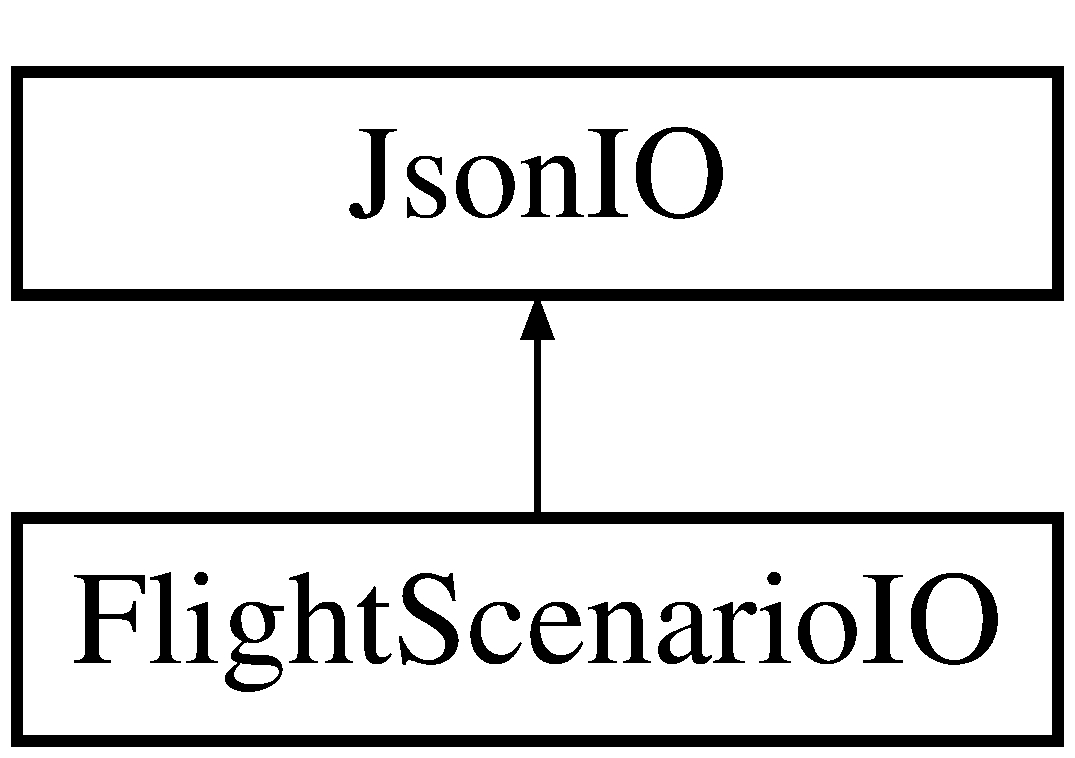
\includegraphics[height=2.000000cm]{class_flight_scenario_i_o}
\end{center}
\end{figure}
\subsection*{Static Public Member Functions}
\begin{DoxyCompactItemize}
\item 
static \hyperlink{class_flight_scenario}{Flight\+Scenario} \hyperlink{class_flight_scenario_i_o_a932ffd37a422cbb044ac1d97866bbc5e}{Read\+File} (std\+::string file\+\_\+name)
\item 
static \hyperlink{class_json_1_1_value}{Json\+::\+Value} \hyperlink{class_flight_scenario_i_o_a725bce8083bc2a390d6bd16860a99892}{Get\+Absolute\+Ownship\+Data} (std\+::string file\+\_\+name)
\item 
static \hyperlink{class_json_1_1_value}{Json\+::\+Value} \hyperlink{class_flight_scenario_i_o_aa5aa3abf7817e22efc7a57a8d422a6c7}{Get\+Flight\+Plans} (std\+::string file\+\_\+name)
\item 
static std\+::vector$<$ std\+::vector$<$ int $>$ $>$ \hyperlink{class_flight_scenario_i_o_a8b9ae191e8c7d182edf553096fbbf72b}{Get\+Start\+Positions} ()
\item 
static std\+::vector$<$ \hyperlink{class_json_1_1_value}{Json\+::\+Value} $>$ \hyperlink{class_flight_scenario_i_o_a65eb5824e5ec0d9790c93ee6abf2166d}{Get\+Flight\+Legs} ()
\item 
static void \hyperlink{class_flight_scenario_i_o_a7f561135d3cc2d7f867bf00acfc6bad1}{Write\+File} (\hyperlink{class_json_1_1_value}{Json\+::\+Value} value)
\end{DoxyCompactItemize}
\subsection*{Additional Inherited Members}


\subsection{Detailed Description}
\hyperlink{class_flight_scenario_i_o}{Flight\+Scenario\+I\+O} is the utility library for reading and writing regarding the \hyperlink{class_flight}{Flight} Scenario files. 

\subsection{Member Function Documentation}
\hypertarget{class_flight_scenario_i_o_a725bce8083bc2a390d6bd16860a99892}{}\index{Flight\+Scenario\+I\+O@{Flight\+Scenario\+I\+O}!Get\+Absolute\+Ownship\+Data@{Get\+Absolute\+Ownship\+Data}}
\index{Get\+Absolute\+Ownship\+Data@{Get\+Absolute\+Ownship\+Data}!Flight\+Scenario\+I\+O@{Flight\+Scenario\+I\+O}}
\subsubsection[{Get\+Absolute\+Ownship\+Data}]{\setlength{\rightskip}{0pt plus 5cm}{\bf Json\+::\+Value} Flight\+Scenario\+I\+O\+::\+Get\+Absolute\+Ownship\+Data (
\begin{DoxyParamCaption}
\item[{std\+::string}]{file\+\_\+name}
\end{DoxyParamCaption}
)\hspace{0.3cm}{\ttfamily [static]}}\label{class_flight_scenario_i_o_a725bce8083bc2a390d6bd16860a99892}
Accessor function to retrieve the initial Ownship data. \begin{DoxyReturn}{Returns}
Initial Ownship data in \hyperlink{class_json_1_1_value}{Json\+::\+Value} form. 
\end{DoxyReturn}
\hypertarget{class_flight_scenario_i_o_a65eb5824e5ec0d9790c93ee6abf2166d}{}\index{Flight\+Scenario\+I\+O@{Flight\+Scenario\+I\+O}!Get\+Flight\+Legs@{Get\+Flight\+Legs}}
\index{Get\+Flight\+Legs@{Get\+Flight\+Legs}!Flight\+Scenario\+I\+O@{Flight\+Scenario\+I\+O}}
\subsubsection[{Get\+Flight\+Legs}]{\setlength{\rightskip}{0pt plus 5cm}static std\+::vector$<${\bf Json\+::\+Value}$>$ Flight\+Scenario\+I\+O\+::\+Get\+Flight\+Legs (
\begin{DoxyParamCaption}
{}
\end{DoxyParamCaption}
)\hspace{0.3cm}{\ttfamily [static]}}\label{class_flight_scenario_i_o_a65eb5824e5ec0d9790c93ee6abf2166d}
Accesor method to all the flight legs. \begin{DoxyReturn}{Returns}
A vector containing all the flight legs in the flight scenario. 
\end{DoxyReturn}
\hypertarget{class_flight_scenario_i_o_aa5aa3abf7817e22efc7a57a8d422a6c7}{}\index{Flight\+Scenario\+I\+O@{Flight\+Scenario\+I\+O}!Get\+Flight\+Plans@{Get\+Flight\+Plans}}
\index{Get\+Flight\+Plans@{Get\+Flight\+Plans}!Flight\+Scenario\+I\+O@{Flight\+Scenario\+I\+O}}
\subsubsection[{Get\+Flight\+Plans}]{\setlength{\rightskip}{0pt plus 5cm}{\bf Json\+::\+Value} Flight\+Scenario\+I\+O\+::\+Get\+Flight\+Plans (
\begin{DoxyParamCaption}
\item[{std\+::string}]{file\+\_\+name}
\end{DoxyParamCaption}
)\hspace{0.3cm}{\ttfamily [static]}}\label{class_flight_scenario_i_o_aa5aa3abf7817e22efc7a57a8d422a6c7}
Accessor function for the list of flight plans. \begin{DoxyReturn}{Returns}
All the flight plans in the J\+S\+O\+N in J\+Son\+::\+Value form. 
\end{DoxyReturn}
\hypertarget{class_flight_scenario_i_o_a8b9ae191e8c7d182edf553096fbbf72b}{}\index{Flight\+Scenario\+I\+O@{Flight\+Scenario\+I\+O}!Get\+Start\+Positions@{Get\+Start\+Positions}}
\index{Get\+Start\+Positions@{Get\+Start\+Positions}!Flight\+Scenario\+I\+O@{Flight\+Scenario\+I\+O}}
\subsubsection[{Get\+Start\+Positions}]{\setlength{\rightskip}{0pt plus 5cm}static std\+::vector$<$std\+::vector$<$int$>$ $>$ Flight\+Scenario\+I\+O\+::\+Get\+Start\+Positions (
\begin{DoxyParamCaption}
{}
\end{DoxyParamCaption}
)\hspace{0.3cm}{\ttfamily [static]}}\label{class_flight_scenario_i_o_a8b9ae191e8c7d182edf553096fbbf72b}
Accessor method to a vector containing the starting positions of all aircrafts. \begin{DoxyReturn}{Returns}
Vector containing the starting positions of all aircrafts 
\end{DoxyReturn}
\hypertarget{class_flight_scenario_i_o_a932ffd37a422cbb044ac1d97866bbc5e}{}\index{Flight\+Scenario\+I\+O@{Flight\+Scenario\+I\+O}!Read\+File@{Read\+File}}
\index{Read\+File@{Read\+File}!Flight\+Scenario\+I\+O@{Flight\+Scenario\+I\+O}}
\subsubsection[{Read\+File}]{\setlength{\rightskip}{0pt plus 5cm}{\bf Flight\+Scenario} Flight\+Scenario\+I\+O\+::\+Read\+File (
\begin{DoxyParamCaption}
\item[{std\+::string}]{file\+\_\+name}
\end{DoxyParamCaption}
)\hspace{0.3cm}{\ttfamily [static]}}\label{class_flight_scenario_i_o_a932ffd37a422cbb044ac1d97866bbc5e}
Reads the J\+S\+O\+N \hyperlink{class_flight_scenario}{Flight\+Scenario} file and returns a reference to the root of the J\+S\+O\+N file. \begin{DoxyReturn}{Returns}
The root of the J\+S\+O\+N File 
\end{DoxyReturn}
\hypertarget{class_flight_scenario_i_o_a7f561135d3cc2d7f867bf00acfc6bad1}{}\index{Flight\+Scenario\+I\+O@{Flight\+Scenario\+I\+O}!Write\+File@{Write\+File}}
\index{Write\+File@{Write\+File}!Flight\+Scenario\+I\+O@{Flight\+Scenario\+I\+O}}
\subsubsection[{Write\+File}]{\setlength{\rightskip}{0pt plus 5cm}static void Flight\+Scenario\+I\+O\+::\+Write\+File (
\begin{DoxyParamCaption}
\item[{{\bf Json\+::\+Value}}]{value}
\end{DoxyParamCaption}
)\hspace{0.3cm}{\ttfamily [static]}}\label{class_flight_scenario_i_o_a7f561135d3cc2d7f867bf00acfc6bad1}
Write specified \hyperlink{class_json_1_1_value}{Json\+::\+Value} to a formatted output log file. 
\begin{DoxyParams}{Parameters}
{\em value} & is the \hyperlink{class_json_1_1_value}{Json\+::\+Value} that you want to log. \\
\hline
\end{DoxyParams}


The documentation for this class was generated from the following files\+:\begin{DoxyCompactItemize}
\item 
/home/fpoole/development/cpe406/saas/lib/jsonio/inc/Flight\+Scenario\+I\+O.\+h\item 
/home/fpoole/development/cpe406/saas/lib/jsonio/src/Flight\+Scenario\+I\+O.\+cpp\end{DoxyCompactItemize}

\hypertarget{classfoo}{}\section{foo Class Reference}
\label{classfoo}\index{foo@{foo}}
\subsection*{Public Member Functions}
\begin{DoxyCompactItemize}
\item 
int {\bfseries get\+Zero} ()\hypertarget{classfoo_a86a78c0e319fbd776c8355cfb6103bd4}{}\label{classfoo_a86a78c0e319fbd776c8355cfb6103bd4}

\end{DoxyCompactItemize}


The documentation for this class was generated from the following files\+:\begin{DoxyCompactItemize}
\item 
/\+Users/\+Dat/\+Clion\+Projects/saas/cdti/src/foo.\+h\item 
/\+Users/\+Dat/\+Clion\+Projects/saas/cdti/src/foo.\+cpp\end{DoxyCompactItemize}

\hypertarget{class_protobuf_tcas_demo_1_1_form1}{}\section{Protobuf\+Tcas\+Demo.\+Form1 Class Reference}
\label{class_protobuf_tcas_demo_1_1_form1}\index{Protobuf\+Tcas\+Demo.\+Form1@{Protobuf\+Tcas\+Demo.\+Form1}}
Inheritance diagram for Protobuf\+Tcas\+Demo.\+Form1\+:\begin{figure}[H]
\begin{center}
\leavevmode
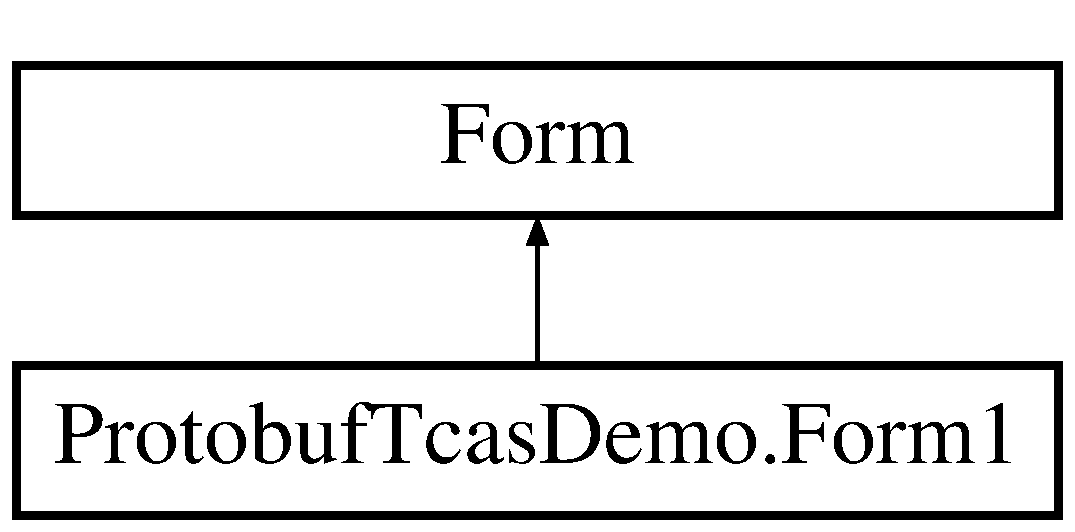
\includegraphics[height=2.000000cm]{class_protobuf_tcas_demo_1_1_form1}
\end{center}
\end{figure}
\subsection*{Protected Member Functions}
\begin{DoxyCompactItemize}
\item 
override void \hyperlink{class_protobuf_tcas_demo_1_1_form1_a6ca94bb508000c9ff866c04156d79712}{Dispose} (bool disposing)
\begin{DoxyCompactList}\small\item\em Clean up any resources being used. \end{DoxyCompactList}\end{DoxyCompactItemize}


\subsection{Member Function Documentation}
\index{Protobuf\+Tcas\+Demo\+::\+Form1@{Protobuf\+Tcas\+Demo\+::\+Form1}!Dispose@{Dispose}}
\index{Dispose@{Dispose}!Protobuf\+Tcas\+Demo\+::\+Form1@{Protobuf\+Tcas\+Demo\+::\+Form1}}
\subsubsection[{\texorpdfstring{Dispose(bool disposing)}{Dispose(bool disposing)}}]{\setlength{\rightskip}{0pt plus 5cm}override void Protobuf\+Tcas\+Demo.\+Form1.\+Dispose (
\begin{DoxyParamCaption}
\item[{bool}]{disposing}
\end{DoxyParamCaption}
)\hspace{0.3cm}{\ttfamily [inline]}, {\ttfamily [protected]}}\hypertarget{class_protobuf_tcas_demo_1_1_form1_a6ca94bb508000c9ff866c04156d79712}{}\label{class_protobuf_tcas_demo_1_1_form1_a6ca94bb508000c9ff866c04156d79712}


Clean up any resources being used. 


\begin{DoxyParams}{Parameters}
{\em disposing} & true if managed resources should be disposed; otherwise, false.\\
\hline
\end{DoxyParams}


The documentation for this class was generated from the following files\+:\begin{DoxyCompactItemize}
\item 
/\+Users/\+Dat/\+Clion\+Projects/saas/cdti/\+Protobuf\+Tcas\+Demo/\+Protobuf\+Tcas\+Demo/Form1.\+cs\item 
/\+Users/\+Dat/\+Clion\+Projects/saas/cdti/\+Protobuf\+Tcas\+Demo/\+Protobuf\+Tcas\+Demo/Form1.\+Designer.\+cs\end{DoxyCompactItemize}

\input{struct_history}
\hypertarget{class_json_i_o}{}\section{Json\+IO Class Reference}
\label{class_json_i_o}\index{Json\+IO@{Json\+IO}}
Inheritance diagram for Json\+IO\+:\begin{figure}[H]
\begin{center}
\leavevmode
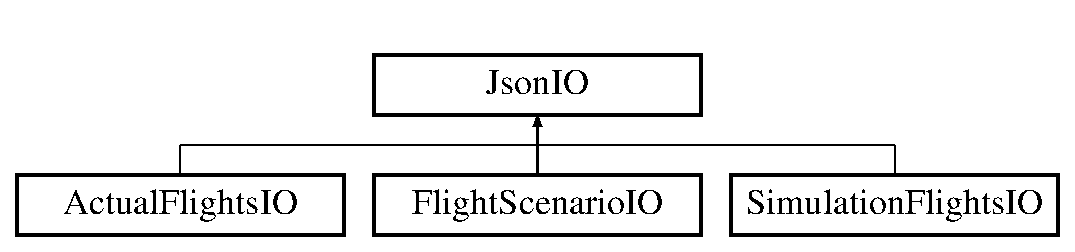
\includegraphics[height=2.000000cm]{class_json_i_o}
\end{center}
\end{figure}
\subsection*{Public Member Functions}
\begin{DoxyCompactItemize}
\item 
virtual void {\bfseries write\+File} (\hyperlink{class_json_1_1_value}{Json\+::\+Value})=0\hypertarget{class_json_i_o_af6f8a61815323ac89752b5365fb2acab}{}\label{class_json_i_o_af6f8a61815323ac89752b5365fb2acab}

\end{DoxyCompactItemize}
\subsection*{Static Public Member Functions}
\begin{DoxyCompactItemize}
\item 
static \hyperlink{class_json_1_1_value}{Json\+::\+Value} {\bfseries read\+File} ()\hypertarget{class_json_i_o_a95a39d392f3f27bb94dc5ad5ef3dba19}{}\label{class_json_i_o_a95a39d392f3f27bb94dc5ad5ef3dba19}

\end{DoxyCompactItemize}


The documentation for this class was generated from the following file\+:\begin{DoxyCompactItemize}
\item 
/\+Users/\+Dat/\+Clion\+Projects/saas/lib/jsonio/inc/Json\+I\+O.\+h\end{DoxyCompactItemize}

\hypertarget{class_silent_orbit_1_1_protocol_buffers_1_1_key}{}\section{Silent\+Orbit.\+Protocol\+Buffers.\+Key Class Reference}
\label{class_silent_orbit_1_1_protocol_buffers_1_1_key}\index{Silent\+Orbit.\+Protocol\+Buffers.\+Key@{Silent\+Orbit.\+Protocol\+Buffers.\+Key}}
\subsection*{Public Member Functions}
\begin{DoxyCompactItemize}
\item 
{\bfseries Key} (uint field, Wire wire\+Type)\hypertarget{class_silent_orbit_1_1_protocol_buffers_1_1_key_afec25f3e95b45ea1637725a855e81360}{}\label{class_silent_orbit_1_1_protocol_buffers_1_1_key_afec25f3e95b45ea1637725a855e81360}

\item 
override string {\bfseries To\+String} ()\hypertarget{class_silent_orbit_1_1_protocol_buffers_1_1_key_ae46395a4028f035c19a07caa680f1ad0}{}\label{class_silent_orbit_1_1_protocol_buffers_1_1_key_ae46395a4028f035c19a07caa680f1ad0}

\item 
{\bfseries Key} (uint field, Wire wire\+Type)\hypertarget{class_silent_orbit_1_1_protocol_buffers_1_1_key_afec25f3e95b45ea1637725a855e81360}{}\label{class_silent_orbit_1_1_protocol_buffers_1_1_key_afec25f3e95b45ea1637725a855e81360}

\item 
override string {\bfseries To\+String} ()\hypertarget{class_silent_orbit_1_1_protocol_buffers_1_1_key_ae46395a4028f035c19a07caa680f1ad0}{}\label{class_silent_orbit_1_1_protocol_buffers_1_1_key_ae46395a4028f035c19a07caa680f1ad0}

\end{DoxyCompactItemize}
\subsection*{Properties}
\begin{DoxyCompactItemize}
\item 
uint {\bfseries Field}\hspace{0.3cm}{\ttfamily  \mbox{[}get, set\mbox{]}}\hypertarget{class_silent_orbit_1_1_protocol_buffers_1_1_key_a633f5ab095f7ed07ae3767d719834747}{}\label{class_silent_orbit_1_1_protocol_buffers_1_1_key_a633f5ab095f7ed07ae3767d719834747}

\item 
Wire {\bfseries Wire\+Type}\hspace{0.3cm}{\ttfamily  \mbox{[}get, set\mbox{]}}\hypertarget{class_silent_orbit_1_1_protocol_buffers_1_1_key_a0080c3bd74cda7b92d7066cdeb25f819}{}\label{class_silent_orbit_1_1_protocol_buffers_1_1_key_a0080c3bd74cda7b92d7066cdeb25f819}

\end{DoxyCompactItemize}


The documentation for this class was generated from the following file\+:\begin{DoxyCompactItemize}
\item 
/home/andrea/\+Clion\+Projects/saas/cdti/\+C\+D\+T\+I\+Unity/\+Assets/scripts/Protocol\+Parser.\+cs\end{DoxyCompactItemize}

\hypertarget{class_silent_orbit_1_1_protocol_buffers_1_1_key_value}{}\section{Silent\+Orbit.\+Protocol\+Buffers.\+Key\+Value Class Reference}
\label{class_silent_orbit_1_1_protocol_buffers_1_1_key_value}\index{Silent\+Orbit.\+Protocol\+Buffers.\+Key\+Value@{Silent\+Orbit.\+Protocol\+Buffers.\+Key\+Value}}


Storage of unknown fields  


\subsection*{Public Member Functions}
\begin{DoxyCompactItemize}
\item 
\hypertarget{class_silent_orbit_1_1_protocol_buffers_1_1_key_value_a0c2f85ee43da09988ea6ce9f265ad471}{}{\bfseries Key\+Value} (\hyperlink{class_silent_orbit_1_1_protocol_buffers_1_1_key}{Key} key, byte\mbox{[}$\,$\mbox{]} value)\label{class_silent_orbit_1_1_protocol_buffers_1_1_key_value_a0c2f85ee43da09988ea6ce9f265ad471}

\item 
\hypertarget{class_silent_orbit_1_1_protocol_buffers_1_1_key_value_a659b764ee7159314181fc2f57547b59c}{}override string {\bfseries To\+String} ()\label{class_silent_orbit_1_1_protocol_buffers_1_1_key_value_a659b764ee7159314181fc2f57547b59c}

\item 
\hypertarget{class_silent_orbit_1_1_protocol_buffers_1_1_key_value_a0c2f85ee43da09988ea6ce9f265ad471}{}{\bfseries Key\+Value} (\hyperlink{class_silent_orbit_1_1_protocol_buffers_1_1_key}{Key} key, byte\mbox{[}$\,$\mbox{]} value)\label{class_silent_orbit_1_1_protocol_buffers_1_1_key_value_a0c2f85ee43da09988ea6ce9f265ad471}

\item 
\hypertarget{class_silent_orbit_1_1_protocol_buffers_1_1_key_value_a659b764ee7159314181fc2f57547b59c}{}override string {\bfseries To\+String} ()\label{class_silent_orbit_1_1_protocol_buffers_1_1_key_value_a659b764ee7159314181fc2f57547b59c}

\end{DoxyCompactItemize}
\subsection*{Properties}
\begin{DoxyCompactItemize}
\item 
\hypertarget{class_silent_orbit_1_1_protocol_buffers_1_1_key_value_a041f3d9740a6df457ea3c74d2b024b7f}{}\hyperlink{class_silent_orbit_1_1_protocol_buffers_1_1_key}{Key} {\bfseries Key}\hspace{0.3cm}{\ttfamily  \mbox{[}get, set\mbox{]}}\label{class_silent_orbit_1_1_protocol_buffers_1_1_key_value_a041f3d9740a6df457ea3c74d2b024b7f}

\item 
\hypertarget{class_silent_orbit_1_1_protocol_buffers_1_1_key_value_a358b40d160e891e8cdd9039d86469f60}{}byte\mbox{[}$\,$\mbox{]} {\bfseries Value}\hspace{0.3cm}{\ttfamily  \mbox{[}get, set\mbox{]}}\label{class_silent_orbit_1_1_protocol_buffers_1_1_key_value_a358b40d160e891e8cdd9039d86469f60}

\end{DoxyCompactItemize}


\subsection{Detailed Description}
Storage of unknown fields 



The documentation for this class was generated from the following file\+:\begin{DoxyCompactItemize}
\item 
/home/fpoole/development/cpe406/saas/cdti/\+C\+D\+T\+I\+Unity/\+Assets/scripts/Protocol\+Parser.\+cs\end{DoxyCompactItemize}

\hypertarget{class_json_1_1_logic_error}{}\section{Json\+:\+:Logic\+Error Class Reference}
\label{class_json_1_1_logic_error}\index{Json\+::\+Logic\+Error@{Json\+::\+Logic\+Error}}


{\ttfamily \#include $<$json.\+h$>$}

Inheritance diagram for Json\+:\+:Logic\+Error\+:\begin{figure}[H]
\begin{center}
\leavevmode
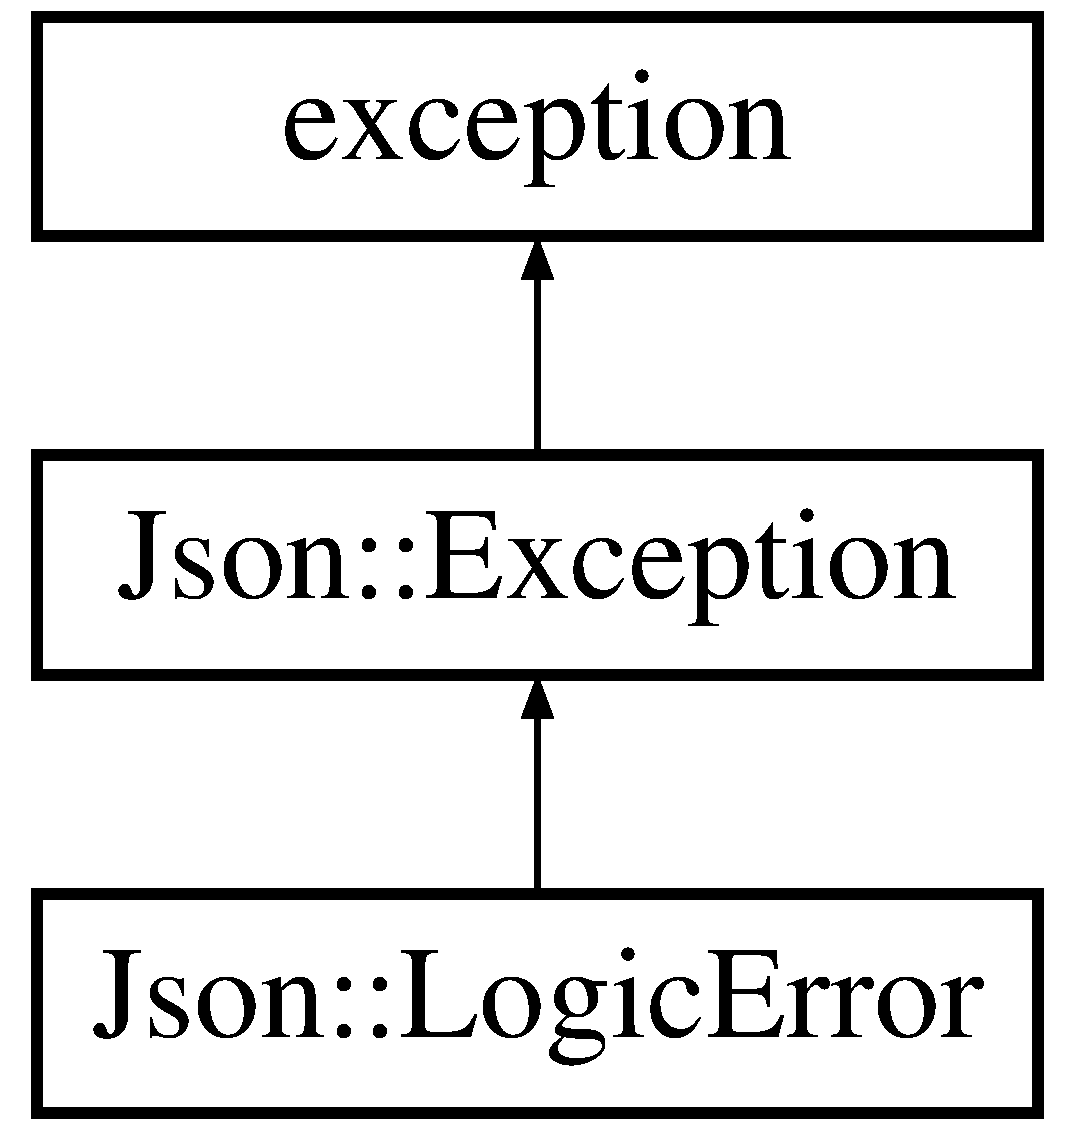
\includegraphics[height=3.000000cm]{class_json_1_1_logic_error}
\end{center}
\end{figure}
\subsection*{Public Member Functions}
\begin{DoxyCompactItemize}
\item 
\hypertarget{class_json_1_1_logic_error_ae8a834c790017a55df74c70b91f23329}{}{\bfseries Logic\+Error} (std\+::string const \&msg)\label{class_json_1_1_logic_error_ae8a834c790017a55df74c70b91f23329}

\end{DoxyCompactItemize}
\subsection*{Additional Inherited Members}


\subsection{Detailed Description}
Exceptions thrown by J\+S\+O\+N\+\_\+\+A\+S\+S\+E\+R\+T/\+J\+S\+O\+N\+\_\+\+F\+A\+I\+L macros.

These are precondition-\/violations (user bugs) and internal errors (our bugs).

\begin{DoxyRemark}{Remarks}
derived from \hyperlink{class_json_1_1_exception}{Json\+::\+Exception} 
\end{DoxyRemark}


The documentation for this class was generated from the following files\+:\begin{DoxyCompactItemize}
\item 
/home/frank/dev/cpe402/saas/lib/jsoncpp/inc/json.\+h\item 
/home/frank/dev/cpe402/saas/lib/jsoncpp/src/jsoncpp.\+cpp\end{DoxyCompactItemize}

\hypertarget{interface_silent_orbit_1_1_protocol_buffers_1_1_memory_stream_stack}{}\section{Silent\+Orbit.\+Protocol\+Buffers.\+Memory\+Stream\+Stack Interface Reference}
\label{interface_silent_orbit_1_1_protocol_buffers_1_1_memory_stream_stack}\index{Silent\+Orbit.\+Protocol\+Buffers.\+Memory\+Stream\+Stack@{Silent\+Orbit.\+Protocol\+Buffers.\+Memory\+Stream\+Stack}}
Inheritance diagram for Silent\+Orbit.\+Protocol\+Buffers.\+Memory\+Stream\+Stack\+:\begin{figure}[H]
\begin{center}
\leavevmode
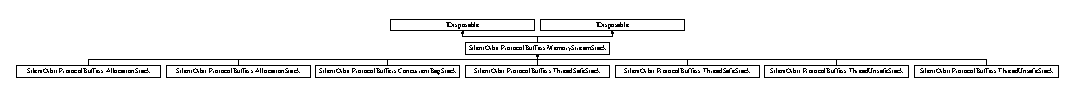
\includegraphics[height=0.821918cm]{interface_silent_orbit_1_1_protocol_buffers_1_1_memory_stream_stack}
\end{center}
\end{figure}
\subsection*{Public Member Functions}
\begin{DoxyCompactItemize}
\item 
\hypertarget{interface_silent_orbit_1_1_protocol_buffers_1_1_memory_stream_stack_a7408e30789e2d7ee77cd166e69b98a48}{}Memory\+Stream {\bfseries Pop} ()\label{interface_silent_orbit_1_1_protocol_buffers_1_1_memory_stream_stack_a7408e30789e2d7ee77cd166e69b98a48}

\item 
\hypertarget{interface_silent_orbit_1_1_protocol_buffers_1_1_memory_stream_stack_a1ae64da82a0acdfaaec81a0697d3c070}{}void {\bfseries Push} (Memory\+Stream stream)\label{interface_silent_orbit_1_1_protocol_buffers_1_1_memory_stream_stack_a1ae64da82a0acdfaaec81a0697d3c070}

\item 
\hypertarget{interface_silent_orbit_1_1_protocol_buffers_1_1_memory_stream_stack_a7408e30789e2d7ee77cd166e69b98a48}{}Memory\+Stream {\bfseries Pop} ()\label{interface_silent_orbit_1_1_protocol_buffers_1_1_memory_stream_stack_a7408e30789e2d7ee77cd166e69b98a48}

\item 
\hypertarget{interface_silent_orbit_1_1_protocol_buffers_1_1_memory_stream_stack_a1ae64da82a0acdfaaec81a0697d3c070}{}void {\bfseries Push} (Memory\+Stream stream)\label{interface_silent_orbit_1_1_protocol_buffers_1_1_memory_stream_stack_a1ae64da82a0acdfaaec81a0697d3c070}

\end{DoxyCompactItemize}


The documentation for this interface was generated from the following file\+:\begin{DoxyCompactItemize}
\item 
/home/frank/dev/cpe402/saas/cdti/\+C\+D\+T\+I\+Unity/\+Assets/scripts/Protocol\+Parser.\+cs\end{DoxyCompactItemize}

\hypertarget{class_example_1_1_msg}{}\section{Example.\+Msg Class Reference}
\label{class_example_1_1_msg}\index{Example.\+Msg@{Example.\+Msg}}
\subsection*{Static Public Member Functions}
\begin{DoxyCompactItemize}
\item 
static \hyperlink{class_example_1_1_msg}{Msg} \hyperlink{class_example_1_1_msg_a80dd17c33b49732e8d696c27d14955d5}{Deserialize} (Stream stream)
\begin{DoxyCompactList}\small\item\em Helper\+: create a new instance to deserializing into\end{DoxyCompactList}\item 
static \hyperlink{class_example_1_1_msg}{Msg} \hyperlink{class_example_1_1_msg_ad21dc5b0d3210a40a3f27db6dd62ac2b}{Deserialize\+Length\+Delimited} (Stream stream)
\begin{DoxyCompactList}\small\item\em Helper\+: create a new instance to deserializing into\end{DoxyCompactList}\item 
static \hyperlink{class_example_1_1_msg}{Msg} \hyperlink{class_example_1_1_msg_a20c91f6ab824db878c0289e98369081a}{Deserialize\+Length} (Stream stream, int length)
\begin{DoxyCompactList}\small\item\em Helper\+: create a new instance to deserializing into\end{DoxyCompactList}\item 
static \hyperlink{class_example_1_1_msg}{Msg} \hyperlink{class_example_1_1_msg_a8070c76dc5a3026a5805b77239769253}{Deserialize} (byte\mbox{[}$\,$\mbox{]} buffer)
\begin{DoxyCompactList}\small\item\em Helper\+: put the buffer into a Memory\+Stream and create a new instance to deserializing into\end{DoxyCompactList}\item 
static \hyperlink{class_example_1_1_msg}{Example.\+Msg} \hyperlink{class_example_1_1_msg_a04fa901ea1daced3b5ba715b692dbf82}{Deserialize} (byte\mbox{[}$\,$\mbox{]} buffer, \hyperlink{class_example_1_1_msg}{Example.\+Msg} instance)
\begin{DoxyCompactList}\small\item\em Helper\+: put the buffer into a Memory\+Stream before deserializing\end{DoxyCompactList}\item 
static \hyperlink{class_example_1_1_msg}{Example.\+Msg} \hyperlink{class_example_1_1_msg_aae32b461bf8880ecc0a02f36079bcd8e}{Deserialize} (Stream stream, \hyperlink{class_example_1_1_msg}{Example.\+Msg} instance)
\begin{DoxyCompactList}\small\item\em Takes the remaining content of the stream and deserialze it into the instance.\end{DoxyCompactList}\item 
static \hyperlink{class_example_1_1_msg}{Example.\+Msg} \hyperlink{class_example_1_1_msg_abb02674ad6bc79321e7731ed966a4799}{Deserialize\+Length\+Delimited} (Stream stream, \hyperlink{class_example_1_1_msg}{Example.\+Msg} instance)
\begin{DoxyCompactList}\small\item\em Read the Var\+Int length prefix and the given number of bytes from the stream and deserialze it into the instance.\end{DoxyCompactList}\item 
static \hyperlink{class_example_1_1_msg}{Example.\+Msg} \hyperlink{class_example_1_1_msg_a50902d520a9e236c8d4d3bdd1a901a28}{Deserialize\+Length} (Stream stream, int length, \hyperlink{class_example_1_1_msg}{Example.\+Msg} instance)
\begin{DoxyCompactList}\small\item\em Read the given number of bytes from the stream and deserialze it into the instance.\end{DoxyCompactList}\item 
static void \hyperlink{class_example_1_1_msg_a49aaee7375865354ce12aedca5a19f8e}{Serialize} (Stream stream, \hyperlink{class_example_1_1_msg}{Msg} instance)
\begin{DoxyCompactList}\small\item\em Serialize the instance into the stream\end{DoxyCompactList}\item 
static byte\mbox{[}$\,$\mbox{]} \hyperlink{class_example_1_1_msg_ad5eca0b03532f735363b71b099db9d2c}{Serialize\+To\+Bytes} (\hyperlink{class_example_1_1_msg}{Msg} instance)
\begin{DoxyCompactList}\small\item\em Helper\+: Serialize into a Memory\+Stream and return its byte array\end{DoxyCompactList}\item 
static void \hyperlink{class_example_1_1_msg_a68a58ceca8838160393c72a1013e78c0}{Serialize\+Length\+Delimited} (Stream stream, \hyperlink{class_example_1_1_msg}{Msg} instance)
\begin{DoxyCompactList}\small\item\em Helper\+: Serialize with a varint length prefix\end{DoxyCompactList}\end{DoxyCompactItemize}
\subsection*{Properties}
\begin{DoxyCompactItemize}
\item 
\hypertarget{class_example_1_1_msg_abc44dced34112e02604436acdc20e10b}{}string {\bfseries Name}\hspace{0.3cm}{\ttfamily  \mbox{[}get, set\mbox{]}}\label{class_example_1_1_msg_abc44dced34112e02604436acdc20e10b}

\item 
\hypertarget{class_example_1_1_msg_ade4a514e1c6528ce00aaab71ce6945b3}{}int {\bfseries Age}\hspace{0.3cm}{\ttfamily  \mbox{[}get, set\mbox{]}}\label{class_example_1_1_msg_ade4a514e1c6528ce00aaab71ce6945b3}

\end{DoxyCompactItemize}


\subsection{Member Function Documentation}
\hypertarget{class_example_1_1_msg_a80dd17c33b49732e8d696c27d14955d5}{}\index{Example\+::\+Msg@{Example\+::\+Msg}!Deserialize@{Deserialize}}
\index{Deserialize@{Deserialize}!Example\+::\+Msg@{Example\+::\+Msg}}
\subsubsection[{Deserialize}]{\setlength{\rightskip}{0pt plus 5cm}static {\bf Msg} Example.\+Msg.\+Deserialize (
\begin{DoxyParamCaption}
\item[{Stream}]{stream}
\end{DoxyParamCaption}
)\hspace{0.3cm}{\ttfamily [inline]}, {\ttfamily [static]}}\label{class_example_1_1_msg_a80dd17c33b49732e8d696c27d14955d5}


Helper\+: create a new instance to deserializing into

\hypertarget{class_example_1_1_msg_a8070c76dc5a3026a5805b77239769253}{}\index{Example\+::\+Msg@{Example\+::\+Msg}!Deserialize@{Deserialize}}
\index{Deserialize@{Deserialize}!Example\+::\+Msg@{Example\+::\+Msg}}
\subsubsection[{Deserialize}]{\setlength{\rightskip}{0pt plus 5cm}static {\bf Msg} Example.\+Msg.\+Deserialize (
\begin{DoxyParamCaption}
\item[{byte\mbox{[}$\,$\mbox{]}}]{buffer}
\end{DoxyParamCaption}
)\hspace{0.3cm}{\ttfamily [inline]}, {\ttfamily [static]}}\label{class_example_1_1_msg_a8070c76dc5a3026a5805b77239769253}


Helper\+: put the buffer into a Memory\+Stream and create a new instance to deserializing into

\hypertarget{class_example_1_1_msg_a04fa901ea1daced3b5ba715b692dbf82}{}\index{Example\+::\+Msg@{Example\+::\+Msg}!Deserialize@{Deserialize}}
\index{Deserialize@{Deserialize}!Example\+::\+Msg@{Example\+::\+Msg}}
\subsubsection[{Deserialize}]{\setlength{\rightskip}{0pt plus 5cm}static {\bf Example.\+Msg} Example.\+Msg.\+Deserialize (
\begin{DoxyParamCaption}
\item[{byte\mbox{[}$\,$\mbox{]}}]{buffer, }
\item[{{\bf Example.\+Msg}}]{instance}
\end{DoxyParamCaption}
)\hspace{0.3cm}{\ttfamily [inline]}, {\ttfamily [static]}}\label{class_example_1_1_msg_a04fa901ea1daced3b5ba715b692dbf82}


Helper\+: put the buffer into a Memory\+Stream before deserializing

\hypertarget{class_example_1_1_msg_aae32b461bf8880ecc0a02f36079bcd8e}{}\index{Example\+::\+Msg@{Example\+::\+Msg}!Deserialize@{Deserialize}}
\index{Deserialize@{Deserialize}!Example\+::\+Msg@{Example\+::\+Msg}}
\subsubsection[{Deserialize}]{\setlength{\rightskip}{0pt plus 5cm}static {\bf Example.\+Msg} Example.\+Msg.\+Deserialize (
\begin{DoxyParamCaption}
\item[{Stream}]{stream, }
\item[{{\bf Example.\+Msg}}]{instance}
\end{DoxyParamCaption}
)\hspace{0.3cm}{\ttfamily [inline]}, {\ttfamily [static]}}\label{class_example_1_1_msg_aae32b461bf8880ecc0a02f36079bcd8e}


Takes the remaining content of the stream and deserialze it into the instance.

\hypertarget{class_example_1_1_msg_a20c91f6ab824db878c0289e98369081a}{}\index{Example\+::\+Msg@{Example\+::\+Msg}!Deserialize\+Length@{Deserialize\+Length}}
\index{Deserialize\+Length@{Deserialize\+Length}!Example\+::\+Msg@{Example\+::\+Msg}}
\subsubsection[{Deserialize\+Length}]{\setlength{\rightskip}{0pt plus 5cm}static {\bf Msg} Example.\+Msg.\+Deserialize\+Length (
\begin{DoxyParamCaption}
\item[{Stream}]{stream, }
\item[{int}]{length}
\end{DoxyParamCaption}
)\hspace{0.3cm}{\ttfamily [inline]}, {\ttfamily [static]}}\label{class_example_1_1_msg_a20c91f6ab824db878c0289e98369081a}


Helper\+: create a new instance to deserializing into

\hypertarget{class_example_1_1_msg_a50902d520a9e236c8d4d3bdd1a901a28}{}\index{Example\+::\+Msg@{Example\+::\+Msg}!Deserialize\+Length@{Deserialize\+Length}}
\index{Deserialize\+Length@{Deserialize\+Length}!Example\+::\+Msg@{Example\+::\+Msg}}
\subsubsection[{Deserialize\+Length}]{\setlength{\rightskip}{0pt plus 5cm}static {\bf Example.\+Msg} Example.\+Msg.\+Deserialize\+Length (
\begin{DoxyParamCaption}
\item[{Stream}]{stream, }
\item[{int}]{length, }
\item[{{\bf Example.\+Msg}}]{instance}
\end{DoxyParamCaption}
)\hspace{0.3cm}{\ttfamily [inline]}, {\ttfamily [static]}}\label{class_example_1_1_msg_a50902d520a9e236c8d4d3bdd1a901a28}


Read the given number of bytes from the stream and deserialze it into the instance.

\hypertarget{class_example_1_1_msg_ad21dc5b0d3210a40a3f27db6dd62ac2b}{}\index{Example\+::\+Msg@{Example\+::\+Msg}!Deserialize\+Length\+Delimited@{Deserialize\+Length\+Delimited}}
\index{Deserialize\+Length\+Delimited@{Deserialize\+Length\+Delimited}!Example\+::\+Msg@{Example\+::\+Msg}}
\subsubsection[{Deserialize\+Length\+Delimited}]{\setlength{\rightskip}{0pt plus 5cm}static {\bf Msg} Example.\+Msg.\+Deserialize\+Length\+Delimited (
\begin{DoxyParamCaption}
\item[{Stream}]{stream}
\end{DoxyParamCaption}
)\hspace{0.3cm}{\ttfamily [inline]}, {\ttfamily [static]}}\label{class_example_1_1_msg_ad21dc5b0d3210a40a3f27db6dd62ac2b}


Helper\+: create a new instance to deserializing into

\hypertarget{class_example_1_1_msg_abb02674ad6bc79321e7731ed966a4799}{}\index{Example\+::\+Msg@{Example\+::\+Msg}!Deserialize\+Length\+Delimited@{Deserialize\+Length\+Delimited}}
\index{Deserialize\+Length\+Delimited@{Deserialize\+Length\+Delimited}!Example\+::\+Msg@{Example\+::\+Msg}}
\subsubsection[{Deserialize\+Length\+Delimited}]{\setlength{\rightskip}{0pt plus 5cm}static {\bf Example.\+Msg} Example.\+Msg.\+Deserialize\+Length\+Delimited (
\begin{DoxyParamCaption}
\item[{Stream}]{stream, }
\item[{{\bf Example.\+Msg}}]{instance}
\end{DoxyParamCaption}
)\hspace{0.3cm}{\ttfamily [inline]}, {\ttfamily [static]}}\label{class_example_1_1_msg_abb02674ad6bc79321e7731ed966a4799}


Read the Var\+Int length prefix and the given number of bytes from the stream and deserialze it into the instance.

\hypertarget{class_example_1_1_msg_a49aaee7375865354ce12aedca5a19f8e}{}\index{Example\+::\+Msg@{Example\+::\+Msg}!Serialize@{Serialize}}
\index{Serialize@{Serialize}!Example\+::\+Msg@{Example\+::\+Msg}}
\subsubsection[{Serialize}]{\setlength{\rightskip}{0pt plus 5cm}static void Example.\+Msg.\+Serialize (
\begin{DoxyParamCaption}
\item[{Stream}]{stream, }
\item[{{\bf Msg}}]{instance}
\end{DoxyParamCaption}
)\hspace{0.3cm}{\ttfamily [inline]}, {\ttfamily [static]}}\label{class_example_1_1_msg_a49aaee7375865354ce12aedca5a19f8e}


Serialize the instance into the stream

\hypertarget{class_example_1_1_msg_a68a58ceca8838160393c72a1013e78c0}{}\index{Example\+::\+Msg@{Example\+::\+Msg}!Serialize\+Length\+Delimited@{Serialize\+Length\+Delimited}}
\index{Serialize\+Length\+Delimited@{Serialize\+Length\+Delimited}!Example\+::\+Msg@{Example\+::\+Msg}}
\subsubsection[{Serialize\+Length\+Delimited}]{\setlength{\rightskip}{0pt plus 5cm}static void Example.\+Msg.\+Serialize\+Length\+Delimited (
\begin{DoxyParamCaption}
\item[{Stream}]{stream, }
\item[{{\bf Msg}}]{instance}
\end{DoxyParamCaption}
)\hspace{0.3cm}{\ttfamily [inline]}, {\ttfamily [static]}}\label{class_example_1_1_msg_a68a58ceca8838160393c72a1013e78c0}


Helper\+: Serialize with a varint length prefix

\hypertarget{class_example_1_1_msg_ad5eca0b03532f735363b71b099db9d2c}{}\index{Example\+::\+Msg@{Example\+::\+Msg}!Serialize\+To\+Bytes@{Serialize\+To\+Bytes}}
\index{Serialize\+To\+Bytes@{Serialize\+To\+Bytes}!Example\+::\+Msg@{Example\+::\+Msg}}
\subsubsection[{Serialize\+To\+Bytes}]{\setlength{\rightskip}{0pt plus 5cm}static byte \mbox{[}$\,$\mbox{]} Example.\+Msg.\+Serialize\+To\+Bytes (
\begin{DoxyParamCaption}
\item[{{\bf Msg}}]{instance}
\end{DoxyParamCaption}
)\hspace{0.3cm}{\ttfamily [inline]}, {\ttfamily [static]}}\label{class_example_1_1_msg_ad5eca0b03532f735363b71b099db9d2c}


Helper\+: Serialize into a Memory\+Stream and return its byte array



The documentation for this class was generated from the following files\+:\begin{DoxyCompactItemize}
\item 
/home/fpoole/development/cpe406/saas/cdti/\+C\+D\+T\+I\+Unity/\+Assets/scripts/Message.\+cs\item 
/home/fpoole/development/cpe406/saas/cdti/\+C\+D\+T\+I\+Unity/\+Assets/scripts/Message.\+Serializer.\+cs\end{DoxyCompactItemize}

\hypertarget{class_network_input}{}\section{Network\+Input Class Reference}
\label{class_network_input}\index{Network\+Input@{Network\+Input}}
Inheritance diagram for Network\+Input\+:\begin{figure}[H]
\begin{center}
\leavevmode
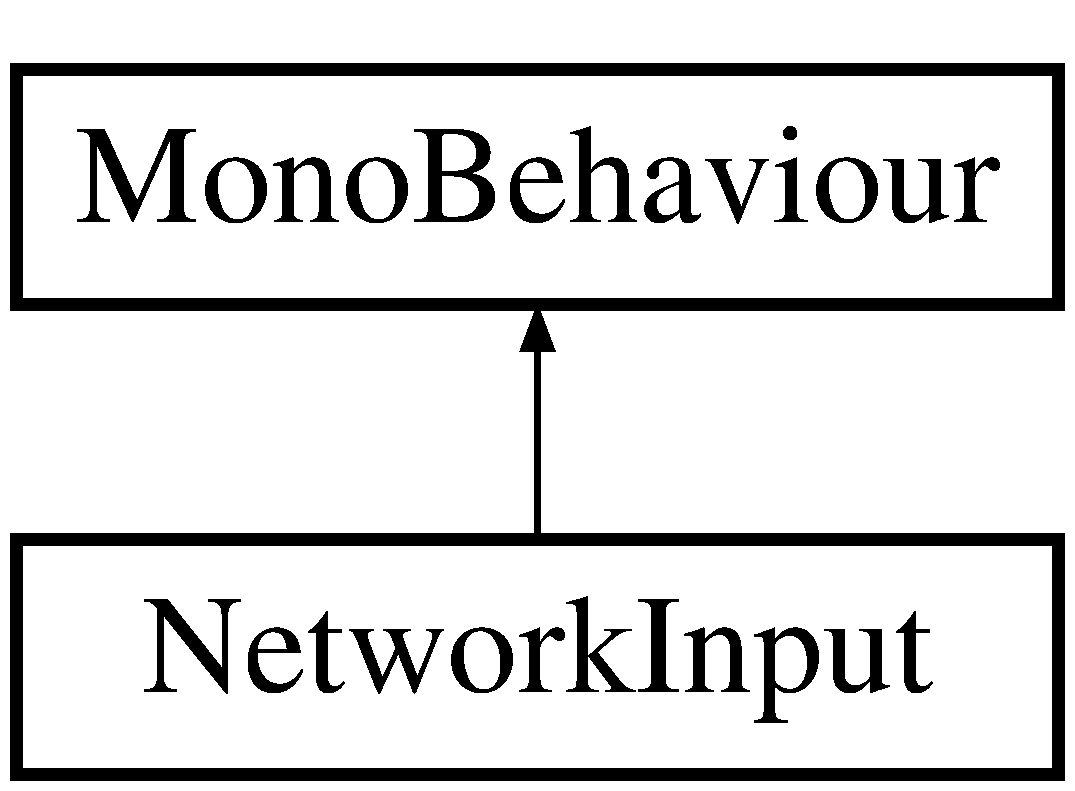
\includegraphics[height=2.000000cm]{class_network_input}
\end{center}
\end{figure}
\subsection*{Public Member Functions}
\begin{DoxyCompactItemize}
\item 
void {\bfseries stop\+Listening} ()\hypertarget{class_network_input_ae14c953e88a3205806cc0b2831ab0859}{}\label{class_network_input_ae14c953e88a3205806cc0b2831ab0859}

\end{DoxyCompactItemize}
\subsection*{Static Public Member Functions}
\begin{DoxyCompactItemize}
\item 
static void {\bfseries logger} (String str)\hypertarget{class_network_input_a3d501d05461b6e9fd05fc7142eadeb1e}{}\label{class_network_input_a3d501d05461b6e9fd05fc7142eadeb1e}

\end{DoxyCompactItemize}
\subsection*{Public Attributes}
\begin{DoxyCompactItemize}
\item 
Sprite {\bfseries air\+Traffic\+Directional}\hypertarget{class_network_input_a645c85b706841b9efd9be62cecff9e37}{}\label{class_network_input_a645c85b706841b9efd9be62cecff9e37}

\item 
Game\+Object {\bfseries aircraft\+Builder}\hypertarget{class_network_input_a4cbaddf7224566f6a01d23a1788b723d}{}\label{class_network_input_a4cbaddf7224566f6a01d23a1788b723d}

\item 
Game\+Object {\bfseries circle}\hypertarget{class_network_input_a8465b038857f973c9a8b7513ead2b563}{}\label{class_network_input_a8465b038857f973c9a8b7513ead2b563}

\item 
int {\bfseries max\+Range} = 20\hypertarget{class_network_input_a3b50fccf39e33592acc615ab7f70abe8}{}\label{class_network_input_a3b50fccf39e33592acc615ab7f70abe8}

\end{DoxyCompactItemize}


The documentation for this class was generated from the following file\+:\begin{DoxyCompactItemize}
\item 
/\+Users/\+Dat/\+Clion\+Projects/saas/cdti/\+C\+D\+T\+I\+Unity/\+Assets/scripts/Network\+Input.\+cs\end{DoxyCompactItemize}

\hypertarget{class_json_1_1_our_char_reader}{}\section{Json\+:\+:Our\+Char\+Reader Class Reference}
\label{class_json_1_1_our_char_reader}\index{Json\+::\+Our\+Char\+Reader@{Json\+::\+Our\+Char\+Reader}}
Inheritance diagram for Json\+:\+:Our\+Char\+Reader\+:\begin{figure}[H]
\begin{center}
\leavevmode
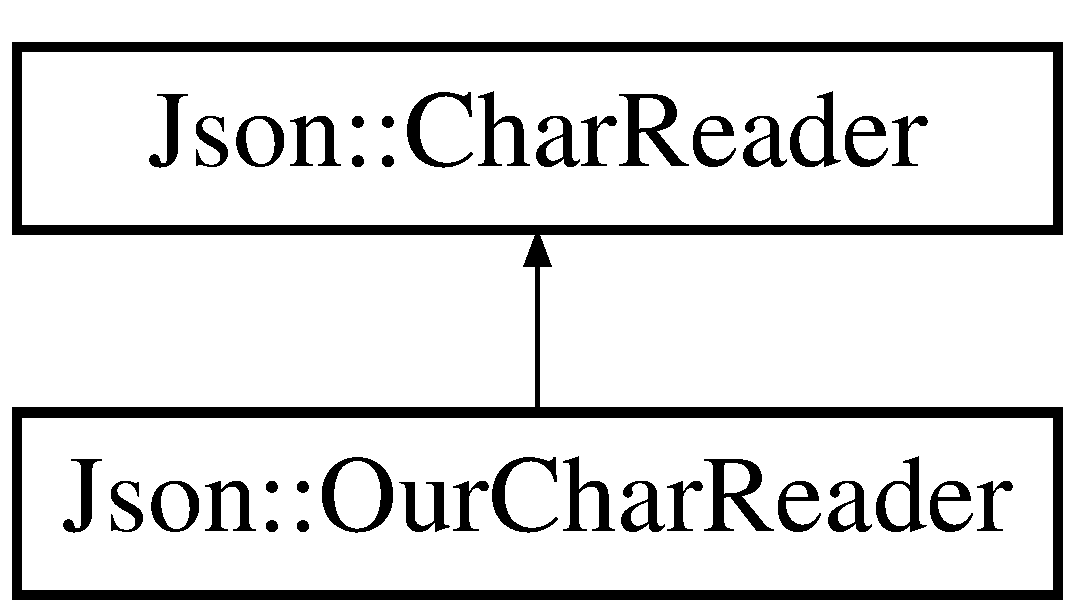
\includegraphics[height=2.000000cm]{class_json_1_1_our_char_reader}
\end{center}
\end{figure}
\subsection*{Public Member Functions}
\begin{DoxyCompactItemize}
\item 
\hypertarget{class_json_1_1_our_char_reader_a5015506620e7ba7bab417756fa1ca9fe}{}{\bfseries Our\+Char\+Reader} (bool collect\+Comments, \hyperlink{class_json_1_1_our_features}{Our\+Features} const \&features)\label{class_json_1_1_our_char_reader_a5015506620e7ba7bab417756fa1ca9fe}

\item 
bool \hyperlink{class_json_1_1_our_char_reader_a52a1fb5fee88d9b63dd462f63b1c9570}{parse} (char const $\ast$begin\+Doc, char const $\ast$end\+Doc, \hyperlink{class_json_1_1_value}{Value} $\ast$root, std\+::string $\ast$errs) override
\begin{DoxyCompactList}\small\item\em Read a \hyperlink{class_json_1_1_value}{Value} from a \href{http://www.json.org}{\tt J\+S\+O\+N} document. The document must be a U\+T\+F-\/8 encoded string containing the document to read. \end{DoxyCompactList}\end{DoxyCompactItemize}


\subsection{Member Function Documentation}
\hypertarget{class_json_1_1_our_char_reader_a52a1fb5fee88d9b63dd462f63b1c9570}{}\index{Json\+::\+Our\+Char\+Reader@{Json\+::\+Our\+Char\+Reader}!parse@{parse}}
\index{parse@{parse}!Json\+::\+Our\+Char\+Reader@{Json\+::\+Our\+Char\+Reader}}
\subsubsection[{parse}]{\setlength{\rightskip}{0pt plus 5cm}bool Json\+::\+Our\+Char\+Reader\+::parse (
\begin{DoxyParamCaption}
\item[{char const $\ast$}]{begin\+Doc, }
\item[{char const $\ast$}]{end\+Doc, }
\item[{{\bf Value} $\ast$}]{root, }
\item[{std\+::string $\ast$}]{errs}
\end{DoxyParamCaption}
)\hspace{0.3cm}{\ttfamily [inline]}, {\ttfamily [override]}, {\ttfamily [virtual]}}\label{class_json_1_1_our_char_reader_a52a1fb5fee88d9b63dd462f63b1c9570}


Read a \hyperlink{class_json_1_1_value}{Value} from a \href{http://www.json.org}{\tt J\+S\+O\+N} document. The document must be a U\+T\+F-\/8 encoded string containing the document to read. 


\begin{DoxyParams}{Parameters}
{\em begin\+Doc} & Pointer on the beginning of the U\+T\+F-\/8 encoded string of the document to read. \\
\hline
{\em end\+Doc} & Pointer on the end of the U\+T\+F-\/8 encoded string of the document to read. Must be $>$= begin\+Doc. \\
\hline
{\em root} & \mbox{[}out\mbox{]} Contains the root value of the document if it was successfully parsed. \\
\hline
{\em errs} & \mbox{[}out\mbox{]} Formatted error messages (if not N\+U\+L\+L) a user friendly string that lists errors in the parsed document. \\
\hline
\end{DoxyParams}
\begin{DoxyReturn}{Returns}
{\ttfamily true} if the document was successfully parsed, {\ttfamily false} if an error occurred. 
\end{DoxyReturn}


Implements \hyperlink{class_json_1_1_char_reader_a48e320be8b13bbc0960cc5808cafec98}{Json\+::\+Char\+Reader}.



The documentation for this class was generated from the following file\+:\begin{DoxyCompactItemize}
\item 
/home/frank/dev/cpe402/saas/lib/jsoncpp/src/jsoncpp.\+cpp\end{DoxyCompactItemize}

\hypertarget{class_json_1_1_our_features}{}\section{Json\+:\+:Our\+Features Class Reference}
\label{class_json_1_1_our_features}\index{Json\+::\+Our\+Features@{Json\+::\+Our\+Features}}
\subsection*{Static Public Member Functions}
\begin{DoxyCompactItemize}
\item 
\hypertarget{class_json_1_1_our_features_a0686e1406b6677f496529f9f3fe98d1e}{}static \hyperlink{class_json_1_1_our_features}{Our\+Features} {\bfseries all} ()\label{class_json_1_1_our_features_a0686e1406b6677f496529f9f3fe98d1e}

\end{DoxyCompactItemize}
\subsection*{Public Attributes}
\begin{DoxyCompactItemize}
\item 
\hypertarget{class_json_1_1_our_features_ac71bb7ba7363d3b05ed76602b036ce33}{}bool {\bfseries allow\+Comments\+\_\+}\label{class_json_1_1_our_features_ac71bb7ba7363d3b05ed76602b036ce33}

\item 
\hypertarget{class_json_1_1_our_features_a2095f66a776c0a4ae6cc931a0c94242e}{}bool {\bfseries strict\+Root\+\_\+}\label{class_json_1_1_our_features_a2095f66a776c0a4ae6cc931a0c94242e}

\item 
\hypertarget{class_json_1_1_our_features_a13963bc44bf948eec1968f7ff8e8f5f1}{}bool {\bfseries allow\+Dropped\+Null\+Placeholders\+\_\+}\label{class_json_1_1_our_features_a13963bc44bf948eec1968f7ff8e8f5f1}

\item 
\hypertarget{class_json_1_1_our_features_af6973fc7e774ce2d634ba99442aeb91a}{}bool {\bfseries allow\+Numeric\+Keys\+\_\+}\label{class_json_1_1_our_features_af6973fc7e774ce2d634ba99442aeb91a}

\item 
\hypertarget{class_json_1_1_our_features_abbd6c196d7a22e2a360a59887eda4610}{}bool {\bfseries allow\+Single\+Quotes\+\_\+}\label{class_json_1_1_our_features_abbd6c196d7a22e2a360a59887eda4610}

\item 
\hypertarget{class_json_1_1_our_features_ae8ad25b90706c78f1a8fe929191ac61b}{}bool {\bfseries fail\+If\+Extra\+\_\+}\label{class_json_1_1_our_features_ae8ad25b90706c78f1a8fe929191ac61b}

\item 
\hypertarget{class_json_1_1_our_features_a39b8e0b86b1c24a45e800c023bb715aa}{}bool {\bfseries reject\+Dup\+Keys\+\_\+}\label{class_json_1_1_our_features_a39b8e0b86b1c24a45e800c023bb715aa}

\item 
\hypertarget{class_json_1_1_our_features_af760f91cc2a7af37e44f78fb466061bb}{}bool {\bfseries allow\+Special\+Floats\+\_\+}\label{class_json_1_1_our_features_af760f91cc2a7af37e44f78fb466061bb}

\item 
\hypertarget{class_json_1_1_our_features_a9a786713902d14be6d57a08cc03ccfff}{}int {\bfseries stack\+Limit\+\_\+}\label{class_json_1_1_our_features_a9a786713902d14be6d57a08cc03ccfff}

\end{DoxyCompactItemize}


The documentation for this class was generated from the following file\+:\begin{DoxyCompactItemize}
\item 
/home/fpoole/development/cpe406/saas/lib/jsoncpp/src/jsoncpp.\+cpp\end{DoxyCompactItemize}

\hypertarget{class_json_1_1_our_reader}{}\section{Json\+:\+:Our\+Reader Class Reference}
\label{class_json_1_1_our_reader}\index{Json\+::\+Our\+Reader@{Json\+::\+Our\+Reader}}
\subsection*{Classes}
\begin{DoxyCompactItemize}
\item 
struct \hyperlink{struct_json_1_1_our_reader_1_1_structured_error}{Structured\+Error}
\end{DoxyCompactItemize}
\subsection*{Public Types}
\begin{DoxyCompactItemize}
\item 
\hypertarget{class_json_1_1_our_reader_a0cd0bab4caa66594ab843ccd5f9dc239}{}typedef char {\bfseries Char}\label{class_json_1_1_our_reader_a0cd0bab4caa66594ab843ccd5f9dc239}

\item 
\hypertarget{class_json_1_1_our_reader_a1bdc7bbc52ba87cae6b19746f2ee0189}{}typedef const Char $\ast$ {\bfseries Location}\label{class_json_1_1_our_reader_a1bdc7bbc52ba87cae6b19746f2ee0189}

\end{DoxyCompactItemize}
\subsection*{Public Member Functions}
\begin{DoxyCompactItemize}
\item 
\hypertarget{class_json_1_1_our_reader_a48a850914b9c8d7781be172930c478e5}{}{\bfseries Our\+Reader} (\hyperlink{class_json_1_1_our_features}{Our\+Features} const \&features)\label{class_json_1_1_our_reader_a48a850914b9c8d7781be172930c478e5}

\item 
\hypertarget{class_json_1_1_our_reader_aba4f8749aab7f02ec17f107e392caf80}{}bool {\bfseries parse} (const char $\ast$begin\+Doc, const char $\ast$end\+Doc, \hyperlink{class_json_1_1_value}{Value} \&root, bool collect\+Comments=true)\label{class_json_1_1_our_reader_aba4f8749aab7f02ec17f107e392caf80}

\item 
\hypertarget{class_json_1_1_our_reader_ae9cbb7dbd9c6c96be37432e8dfa1afcb}{}std\+::string {\bfseries get\+Formatted\+Error\+Messages} () const \label{class_json_1_1_our_reader_ae9cbb7dbd9c6c96be37432e8dfa1afcb}

\item 
\hypertarget{class_json_1_1_our_reader_a02ef7871af3706754a233c36e6d489e9}{}std\+::vector$<$ \hyperlink{struct_json_1_1_our_reader_1_1_structured_error}{Structured\+Error} $>$ {\bfseries get\+Structured\+Errors} () const \label{class_json_1_1_our_reader_a02ef7871af3706754a233c36e6d489e9}

\item 
\hypertarget{class_json_1_1_our_reader_aef7aa4ca22ffaa38c401b16951d20e1e}{}bool {\bfseries push\+Error} (const \hyperlink{class_json_1_1_value}{Value} \&value, const std\+::string \&message)\label{class_json_1_1_our_reader_aef7aa4ca22ffaa38c401b16951d20e1e}

\item 
\hypertarget{class_json_1_1_our_reader_ad43315cbb0d6804e3b7177e84a1ec53d}{}bool {\bfseries push\+Error} (const \hyperlink{class_json_1_1_value}{Value} \&value, const std\+::string \&message, const \hyperlink{class_json_1_1_value}{Value} \&extra)\label{class_json_1_1_our_reader_ad43315cbb0d6804e3b7177e84a1ec53d}

\item 
\hypertarget{class_json_1_1_our_reader_a048346238d703ad9aed06beb686e6102}{}bool {\bfseries good} () const \label{class_json_1_1_our_reader_a048346238d703ad9aed06beb686e6102}

\end{DoxyCompactItemize}


The documentation for this class was generated from the following file\+:\begin{DoxyCompactItemize}
\item 
/home/fpoole/development/cpe406/saas/lib/jsoncpp/src/jsoncpp.\+cpp\end{DoxyCompactItemize}

\hypertarget{class_json_1_1_path}{}\section{Json\+:\+:Path Class Reference}
\label{class_json_1_1_path}\index{Json\+::\+Path@{Json\+::\+Path}}


Experimental and untested\+: represents a \char`\"{}path\char`\"{} to access a node.  




{\ttfamily \#include $<$json.\+h$>$}

\subsection*{Public Member Functions}
\begin{DoxyCompactItemize}
\item 
\hypertarget{class_json_1_1_path_aaa37a99650e770d0cd680bf53585ec99}{}{\bfseries Path} (const std\+::string \&path, const \hyperlink{class_json_1_1_path_argument}{Path\+Argument} \&a1=\hyperlink{class_json_1_1_path_argument}{Path\+Argument}(), const \hyperlink{class_json_1_1_path_argument}{Path\+Argument} \&a2=\hyperlink{class_json_1_1_path_argument}{Path\+Argument}(), const \hyperlink{class_json_1_1_path_argument}{Path\+Argument} \&a3=\hyperlink{class_json_1_1_path_argument}{Path\+Argument}(), const \hyperlink{class_json_1_1_path_argument}{Path\+Argument} \&a4=\hyperlink{class_json_1_1_path_argument}{Path\+Argument}(), const \hyperlink{class_json_1_1_path_argument}{Path\+Argument} \&a5=\hyperlink{class_json_1_1_path_argument}{Path\+Argument}())\label{class_json_1_1_path_aaa37a99650e770d0cd680bf53585ec99}

\item 
\hypertarget{class_json_1_1_path_ae1d05fa985a6ee3c57f2b8ed186b5982}{}const \hyperlink{class_json_1_1_value}{Value} \& {\bfseries resolve} (const \hyperlink{class_json_1_1_value}{Value} \&root) const \label{class_json_1_1_path_ae1d05fa985a6ee3c57f2b8ed186b5982}

\item 
\hypertarget{class_json_1_1_path_a33d1749770a4cf74e9a3de419bc7febe}{}\hyperlink{class_json_1_1_value}{Value} {\bfseries resolve} (const \hyperlink{class_json_1_1_value}{Value} \&root, const \hyperlink{class_json_1_1_value}{Value} \&default\+Value) const \label{class_json_1_1_path_a33d1749770a4cf74e9a3de419bc7febe}

\item 
\hyperlink{class_json_1_1_value}{Value} \& \hyperlink{class_json_1_1_path_a5289901fc58ad1fdca1de7fb5a0b620c}{make} (\hyperlink{class_json_1_1_value}{Value} \&root) const 
\end{DoxyCompactItemize}


\subsection{Detailed Description}
Experimental and untested\+: represents a \char`\"{}path\char`\"{} to access a node. 

Syntax\+:
\begin{DoxyItemize}
\item \char`\"{}.\char`\"{} =$>$ root node
\item \char`\"{}.\mbox{[}n\mbox{]}\char`\"{} =$>$ elements at index \textquotesingle{}n\textquotesingle{} of root node (an array value)
\item \char`\"{}.\+name\char`\"{} =$>$ member named \textquotesingle{}name\textquotesingle{} of root node (an object value)
\item \char`\"{}.\+name1.\+name2.\+name3\char`\"{}
\item \char`\"{}.\mbox{[}0\mbox{]}\mbox{[}1\mbox{]}\mbox{[}2\mbox{]}.\+name1\mbox{[}3\mbox{]}\char`\"{}
\item \char`\"{}.\%\char`\"{} =$>$ member name is provided as parameter
\item \char`\"{}.\mbox{[}\%\mbox{]}\char`\"{} =$>$ index is provied as parameter 
\end{DoxyItemize}

\subsection{Member Function Documentation}
\hypertarget{class_json_1_1_path_a5289901fc58ad1fdca1de7fb5a0b620c}{}\index{Json\+::\+Path@{Json\+::\+Path}!make@{make}}
\index{make@{make}!Json\+::\+Path@{Json\+::\+Path}}
\subsubsection[{make}]{\setlength{\rightskip}{0pt plus 5cm}{\bf Value} \& Json\+::\+Path\+::make (
\begin{DoxyParamCaption}
\item[{{\bf Value} \&}]{root}
\end{DoxyParamCaption}
) const}\label{class_json_1_1_path_a5289901fc58ad1fdca1de7fb5a0b620c}
Creates the \char`\"{}path\char`\"{} to access the specified node and returns a reference on the node. 

The documentation for this class was generated from the following files\+:\begin{DoxyCompactItemize}
\item 
/home/frank/dev/cpe402/saas/lib/jsoncpp/inc/json.\+h\item 
/home/frank/dev/cpe402/saas/lib/jsoncpp/src/jsoncpp.\+cpp\end{DoxyCompactItemize}

\hypertarget{class_json_1_1_path_argument}{}\section{Json\+:\+:Path\+Argument Class Reference}
\label{class_json_1_1_path_argument}\index{Json\+::\+Path\+Argument@{Json\+::\+Path\+Argument}}


Experimental and untested\+: represents an element of the \char`\"{}path\char`\"{} to access a node.  




{\ttfamily \#include $<$json.\+h$>$}

\subsection*{Public Member Functions}
\begin{DoxyCompactItemize}
\item 
{\bfseries Path\+Argument} (Array\+Index index)\hypertarget{class_json_1_1_path_argument_a53c5b27143b161301b95fd544c139ecf}{}\label{class_json_1_1_path_argument_a53c5b27143b161301b95fd544c139ecf}

\item 
{\bfseries Path\+Argument} (const char $\ast$key)\hypertarget{class_json_1_1_path_argument_a9690417a8a40e6e49f2acdf6c9281345}{}\label{class_json_1_1_path_argument_a9690417a8a40e6e49f2acdf6c9281345}

\item 
{\bfseries Path\+Argument} (const std\+::string \&key)\hypertarget{class_json_1_1_path_argument_a08f872cfee4fc600f7fa3bcaaff0d41c}{}\label{class_json_1_1_path_argument_a08f872cfee4fc600f7fa3bcaaff0d41c}

\end{DoxyCompactItemize}
\subsection*{Friends}
\begin{DoxyCompactItemize}
\item 
class {\bfseries Path}\hypertarget{class_json_1_1_path_argument_a4877239a6b7f09fbf5a61ca68a49d74c}{}\label{class_json_1_1_path_argument_a4877239a6b7f09fbf5a61ca68a49d74c}

\end{DoxyCompactItemize}


\subsection{Detailed Description}
Experimental and untested\+: represents an element of the \char`\"{}path\char`\"{} to access a node. 

The documentation for this class was generated from the following files\+:\begin{DoxyCompactItemize}
\item 
/\+Users/\+Dat/\+Clion\+Projects/saas/lib/jsoncpp/inc/json.\+h\item 
/\+Users/\+Dat/\+Clion\+Projects/saas/lib/jsoncpp/src/jsoncpp.\+cpp\end{DoxyCompactItemize}

\hypertarget{class_silent_orbit_1_1_protocol_buffers_1_1_position_stream}{}\section{Silent\+Orbit.\+Protocol\+Buffers.\+Position\+Stream Class Reference}
\label{class_silent_orbit_1_1_protocol_buffers_1_1_position_stream}\index{Silent\+Orbit.\+Protocol\+Buffers.\+Position\+Stream@{Silent\+Orbit.\+Protocol\+Buffers.\+Position\+Stream}}


Wrapper for streams that does not support the Position property. Adds support for the Position property.  


Inheritance diagram for Silent\+Orbit.\+Protocol\+Buffers.\+Position\+Stream\+:\begin{figure}[H]
\begin{center}
\leavevmode
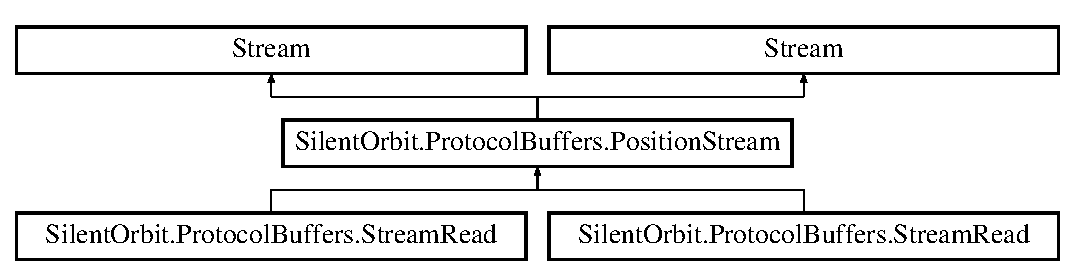
\includegraphics[height=3.000000cm]{class_silent_orbit_1_1_protocol_buffers_1_1_position_stream}
\end{center}
\end{figure}
\subsection*{Public Member Functions}
\begin{DoxyCompactItemize}
\item 
\hyperlink{class_silent_orbit_1_1_protocol_buffers_1_1_position_stream_ab13f95fb3f0983f82388afb9bb1c013c}{Position\+Stream} (Stream base\+Stream)
\begin{DoxyCompactList}\small\item\em Define how many bytes are allowed to read \end{DoxyCompactList}\item 
override void {\bfseries Flush} ()\hypertarget{class_silent_orbit_1_1_protocol_buffers_1_1_position_stream_a6d7ebc2f64c2ca0082999b789e212b34}{}\label{class_silent_orbit_1_1_protocol_buffers_1_1_position_stream_a6d7ebc2f64c2ca0082999b789e212b34}

\item 
override int {\bfseries Read} (byte\mbox{[}$\,$\mbox{]} buffer, int offset, int count)\hypertarget{class_silent_orbit_1_1_protocol_buffers_1_1_position_stream_a27fc475b69fe19b99f006e60b7014dad}{}\label{class_silent_orbit_1_1_protocol_buffers_1_1_position_stream_a27fc475b69fe19b99f006e60b7014dad}

\item 
override int {\bfseries Read\+Byte} ()\hypertarget{class_silent_orbit_1_1_protocol_buffers_1_1_position_stream_aea646d55f92a44b21539362b8aa10a1e}{}\label{class_silent_orbit_1_1_protocol_buffers_1_1_position_stream_aea646d55f92a44b21539362b8aa10a1e}

\item 
override long {\bfseries Seek} (long offset, Seek\+Origin origin)\hypertarget{class_silent_orbit_1_1_protocol_buffers_1_1_position_stream_abf4fc317b09470675d7590be0006c60c}{}\label{class_silent_orbit_1_1_protocol_buffers_1_1_position_stream_abf4fc317b09470675d7590be0006c60c}

\item 
override void {\bfseries Set\+Length} (long value)\hypertarget{class_silent_orbit_1_1_protocol_buffers_1_1_position_stream_a1426c80a536ff433af9000a9b230fe88}{}\label{class_silent_orbit_1_1_protocol_buffers_1_1_position_stream_a1426c80a536ff433af9000a9b230fe88}

\item 
override void {\bfseries Write} (byte\mbox{[}$\,$\mbox{]} buffer, int offset, int count)\hypertarget{class_silent_orbit_1_1_protocol_buffers_1_1_position_stream_a8d3b71fb0c9d731b928ca1d597fdbd97}{}\label{class_silent_orbit_1_1_protocol_buffers_1_1_position_stream_a8d3b71fb0c9d731b928ca1d597fdbd97}

\item 
override void {\bfseries Close} ()\hypertarget{class_silent_orbit_1_1_protocol_buffers_1_1_position_stream_a2aa20011c1749de98505e605f8463fc5}{}\label{class_silent_orbit_1_1_protocol_buffers_1_1_position_stream_a2aa20011c1749de98505e605f8463fc5}

\item 
\hyperlink{class_silent_orbit_1_1_protocol_buffers_1_1_position_stream_ab13f95fb3f0983f82388afb9bb1c013c}{Position\+Stream} (Stream base\+Stream)
\begin{DoxyCompactList}\small\item\em Define how many bytes are allowed to read \end{DoxyCompactList}\item 
override void {\bfseries Flush} ()\hypertarget{class_silent_orbit_1_1_protocol_buffers_1_1_position_stream_a6d7ebc2f64c2ca0082999b789e212b34}{}\label{class_silent_orbit_1_1_protocol_buffers_1_1_position_stream_a6d7ebc2f64c2ca0082999b789e212b34}

\item 
override int {\bfseries Read} (byte\mbox{[}$\,$\mbox{]} buffer, int offset, int count)\hypertarget{class_silent_orbit_1_1_protocol_buffers_1_1_position_stream_a27fc475b69fe19b99f006e60b7014dad}{}\label{class_silent_orbit_1_1_protocol_buffers_1_1_position_stream_a27fc475b69fe19b99f006e60b7014dad}

\item 
override int {\bfseries Read\+Byte} ()\hypertarget{class_silent_orbit_1_1_protocol_buffers_1_1_position_stream_aea646d55f92a44b21539362b8aa10a1e}{}\label{class_silent_orbit_1_1_protocol_buffers_1_1_position_stream_aea646d55f92a44b21539362b8aa10a1e}

\item 
override long {\bfseries Seek} (long offset, Seek\+Origin origin)\hypertarget{class_silent_orbit_1_1_protocol_buffers_1_1_position_stream_abf4fc317b09470675d7590be0006c60c}{}\label{class_silent_orbit_1_1_protocol_buffers_1_1_position_stream_abf4fc317b09470675d7590be0006c60c}

\item 
override void {\bfseries Set\+Length} (long value)\hypertarget{class_silent_orbit_1_1_protocol_buffers_1_1_position_stream_a1426c80a536ff433af9000a9b230fe88}{}\label{class_silent_orbit_1_1_protocol_buffers_1_1_position_stream_a1426c80a536ff433af9000a9b230fe88}

\item 
override void {\bfseries Write} (byte\mbox{[}$\,$\mbox{]} buffer, int offset, int count)\hypertarget{class_silent_orbit_1_1_protocol_buffers_1_1_position_stream_a8d3b71fb0c9d731b928ca1d597fdbd97}{}\label{class_silent_orbit_1_1_protocol_buffers_1_1_position_stream_a8d3b71fb0c9d731b928ca1d597fdbd97}

\item 
override void {\bfseries Close} ()\hypertarget{class_silent_orbit_1_1_protocol_buffers_1_1_position_stream_a2aa20011c1749de98505e605f8463fc5}{}\label{class_silent_orbit_1_1_protocol_buffers_1_1_position_stream_a2aa20011c1749de98505e605f8463fc5}

\end{DoxyCompactItemize}
\subsection*{Protected Member Functions}
\begin{DoxyCompactItemize}
\item 
override void {\bfseries Dispose} (bool disposing)\hypertarget{class_silent_orbit_1_1_protocol_buffers_1_1_position_stream_a78d07ace32dc662ce6388f52d24bd399}{}\label{class_silent_orbit_1_1_protocol_buffers_1_1_position_stream_a78d07ace32dc662ce6388f52d24bd399}

\item 
override void {\bfseries Dispose} (bool disposing)\hypertarget{class_silent_orbit_1_1_protocol_buffers_1_1_position_stream_a78d07ace32dc662ce6388f52d24bd399}{}\label{class_silent_orbit_1_1_protocol_buffers_1_1_position_stream_a78d07ace32dc662ce6388f52d24bd399}

\end{DoxyCompactItemize}
\subsection*{Properties}
\begin{DoxyCompactItemize}
\item 
int \hyperlink{class_silent_orbit_1_1_protocol_buffers_1_1_position_stream_a25ce5053a4a1a394f36344814c8ee785}{Bytes\+Read}\hspace{0.3cm}{\ttfamily  \mbox{[}get\mbox{]}}
\begin{DoxyCompactList}\small\item\em Bytes left to read \end{DoxyCompactList}\item 
override bool {\bfseries Can\+Read}\hspace{0.3cm}{\ttfamily  \mbox{[}get\mbox{]}}\hypertarget{class_silent_orbit_1_1_protocol_buffers_1_1_position_stream_ade46e919badf0142a85e9c8b5f04b69c}{}\label{class_silent_orbit_1_1_protocol_buffers_1_1_position_stream_ade46e919badf0142a85e9c8b5f04b69c}

\item 
override bool {\bfseries Can\+Seek}\hspace{0.3cm}{\ttfamily  \mbox{[}get\mbox{]}}\hypertarget{class_silent_orbit_1_1_protocol_buffers_1_1_position_stream_aaeb77021723c399f173746f6de6972f2}{}\label{class_silent_orbit_1_1_protocol_buffers_1_1_position_stream_aaeb77021723c399f173746f6de6972f2}

\item 
override bool {\bfseries Can\+Write}\hspace{0.3cm}{\ttfamily  \mbox{[}get\mbox{]}}\hypertarget{class_silent_orbit_1_1_protocol_buffers_1_1_position_stream_a664bb30b8fc748e17ad6525a0bf3fc22}{}\label{class_silent_orbit_1_1_protocol_buffers_1_1_position_stream_a664bb30b8fc748e17ad6525a0bf3fc22}

\item 
override long {\bfseries Length}\hspace{0.3cm}{\ttfamily  \mbox{[}get\mbox{]}}\hypertarget{class_silent_orbit_1_1_protocol_buffers_1_1_position_stream_a17e9de092fbbc0b7087e5e0e2326d100}{}\label{class_silent_orbit_1_1_protocol_buffers_1_1_position_stream_a17e9de092fbbc0b7087e5e0e2326d100}

\item 
override long {\bfseries Position}\hspace{0.3cm}{\ttfamily  \mbox{[}get, set\mbox{]}}\hypertarget{class_silent_orbit_1_1_protocol_buffers_1_1_position_stream_a2063b5b768fa0c330c96701cc79293dc}{}\label{class_silent_orbit_1_1_protocol_buffers_1_1_position_stream_a2063b5b768fa0c330c96701cc79293dc}

\end{DoxyCompactItemize}


\subsection{Detailed Description}
Wrapper for streams that does not support the Position property. Adds support for the Position property. 



\subsection{Constructor \& Destructor Documentation}
\index{Silent\+Orbit\+::\+Protocol\+Buffers\+::\+Position\+Stream@{Silent\+Orbit\+::\+Protocol\+Buffers\+::\+Position\+Stream}!Position\+Stream@{Position\+Stream}}
\index{Position\+Stream@{Position\+Stream}!Silent\+Orbit\+::\+Protocol\+Buffers\+::\+Position\+Stream@{Silent\+Orbit\+::\+Protocol\+Buffers\+::\+Position\+Stream}}
\subsubsection[{\texorpdfstring{Position\+Stream(\+Stream base\+Stream)}{PositionStream(Stream baseStream)}}]{\setlength{\rightskip}{0pt plus 5cm}Silent\+Orbit.\+Protocol\+Buffers.\+Position\+Stream.\+Position\+Stream (
\begin{DoxyParamCaption}
\item[{Stream}]{base\+Stream}
\end{DoxyParamCaption}
)\hspace{0.3cm}{\ttfamily [inline]}}\hypertarget{class_silent_orbit_1_1_protocol_buffers_1_1_position_stream_ab13f95fb3f0983f82388afb9bb1c013c}{}\label{class_silent_orbit_1_1_protocol_buffers_1_1_position_stream_ab13f95fb3f0983f82388afb9bb1c013c}


Define how many bytes are allowed to read 


\begin{DoxyParams}{Parameters}
{\em base\+Stream} & Base stream. \\
\hline
{\em max\+Length} & Max length allowed to read from the stream. \\
\hline
\end{DoxyParams}
\index{Silent\+Orbit\+::\+Protocol\+Buffers\+::\+Position\+Stream@{Silent\+Orbit\+::\+Protocol\+Buffers\+::\+Position\+Stream}!Position\+Stream@{Position\+Stream}}
\index{Position\+Stream@{Position\+Stream}!Silent\+Orbit\+::\+Protocol\+Buffers\+::\+Position\+Stream@{Silent\+Orbit\+::\+Protocol\+Buffers\+::\+Position\+Stream}}
\subsubsection[{\texorpdfstring{Position\+Stream(\+Stream base\+Stream)}{PositionStream(Stream baseStream)}}]{\setlength{\rightskip}{0pt plus 5cm}Silent\+Orbit.\+Protocol\+Buffers.\+Position\+Stream.\+Position\+Stream (
\begin{DoxyParamCaption}
\item[{Stream}]{base\+Stream}
\end{DoxyParamCaption}
)\hspace{0.3cm}{\ttfamily [inline]}}\hypertarget{class_silent_orbit_1_1_protocol_buffers_1_1_position_stream_ab13f95fb3f0983f82388afb9bb1c013c}{}\label{class_silent_orbit_1_1_protocol_buffers_1_1_position_stream_ab13f95fb3f0983f82388afb9bb1c013c}


Define how many bytes are allowed to read 


\begin{DoxyParams}{Parameters}
{\em base\+Stream} & Base stream. \\
\hline
{\em max\+Length} & Max length allowed to read from the stream. \\
\hline
\end{DoxyParams}


\subsection{Property Documentation}
\index{Silent\+Orbit\+::\+Protocol\+Buffers\+::\+Position\+Stream@{Silent\+Orbit\+::\+Protocol\+Buffers\+::\+Position\+Stream}!Bytes\+Read@{Bytes\+Read}}
\index{Bytes\+Read@{Bytes\+Read}!Silent\+Orbit\+::\+Protocol\+Buffers\+::\+Position\+Stream@{Silent\+Orbit\+::\+Protocol\+Buffers\+::\+Position\+Stream}}
\subsubsection[{\texorpdfstring{Bytes\+Read}{BytesRead}}]{\setlength{\rightskip}{0pt plus 5cm}int Silent\+Orbit.\+Protocol\+Buffers.\+Position\+Stream.\+Bytes\+Read\hspace{0.3cm}{\ttfamily [get]}}\hypertarget{class_silent_orbit_1_1_protocol_buffers_1_1_position_stream_a25ce5053a4a1a394f36344814c8ee785}{}\label{class_silent_orbit_1_1_protocol_buffers_1_1_position_stream_a25ce5053a4a1a394f36344814c8ee785}


Bytes left to read 



The documentation for this class was generated from the following file\+:\begin{DoxyCompactItemize}
\item 
/home/andrea/\+Clion\+Projects/saas/cdti/\+C\+D\+T\+I\+Unity/\+Assets/scripts/Protocol\+Parser.\+cs\end{DoxyCompactItemize}

\hypertarget{class_protobuf_socket_serializer}{}\section{Protobuf\+Socket\+Serializer Class Reference}
\label{class_protobuf_socket_serializer}\index{Protobuf\+Socket\+Serializer@{Protobuf\+Socket\+Serializer}}


{\ttfamily \#include $<$Protobuf\+Socket\+Serializer.\+h$>$}

\subsection*{Static Public Member Functions}
\begin{DoxyCompactItemize}
\item 
static size\+\_\+t \hyperlink{class_protobuf_socket_serializer_a37206eb18b2b1300b8fab46acd82bdde}{serialize} (const \+::google\+::protobuf\+::\+Message \&msg, char $\ast$\&packet)
\end{DoxyCompactItemize}


\subsection{Detailed Description}
The protocol buffer socket serializer is used to encode header data into any protocol buffer. The header is four bytes containing the length of the buffer data. 

\subsection{Member Function Documentation}
\hypertarget{class_protobuf_socket_serializer_a37206eb18b2b1300b8fab46acd82bdde}{}\index{Protobuf\+Socket\+Serializer@{Protobuf\+Socket\+Serializer}!serialize@{serialize}}
\index{serialize@{serialize}!Protobuf\+Socket\+Serializer@{Protobuf\+Socket\+Serializer}}
\subsubsection[{serialize}]{\setlength{\rightskip}{0pt plus 5cm}size\+\_\+t Protobuf\+Socket\+Serializer\+::serialize (
\begin{DoxyParamCaption}
\item[{const \+::google\+::protobuf\+::\+Message \&}]{msg, }
\item[{char $\ast$\&}]{packet}
\end{DoxyParamCaption}
)\hspace{0.3cm}{\ttfamily [static]}}\label{class_protobuf_socket_serializer_a37206eb18b2b1300b8fab46acd82bdde}
Serialize data for sending over a socket. 
\begin{DoxyParams}{Parameters}
{\em msg} & the protocol buffer message \\
\hline
{\em packet} & The data buffer to write data into \\
\hline
\end{DoxyParams}
\begin{DoxyReturn}{Returns}
the number of bytes encoded 
\end{DoxyReturn}


The documentation for this class was generated from the following files\+:\begin{DoxyCompactItemize}
\item 
/home/frank/dev/cpe402/saas/lib/network/inc/Protobuf\+Socket\+Serializer.\+h\item 
/home/frank/dev/cpe402/saas/lib/network/src/Protobuf\+Socket\+Serializer.\+cpp\end{DoxyCompactItemize}

\hypertarget{class_silent_orbit_1_1_protocol_buffers_1_1_protocol_buffer_exception}{}\section{Silent\+Orbit.\+Protocol\+Buffers.\+Protocol\+Buffer\+Exception Class Reference}
\label{class_silent_orbit_1_1_protocol_buffers_1_1_protocol_buffer_exception}\index{Silent\+Orbit.\+Protocol\+Buffers.\+Protocol\+Buffer\+Exception@{Silent\+Orbit.\+Protocol\+Buffers.\+Protocol\+Buffer\+Exception}}


$>$ This exception is thrown when badly formatted protocol buffer data is read. /summary$>$  


Inheritance diagram for Silent\+Orbit.\+Protocol\+Buffers.\+Protocol\+Buffer\+Exception\+:\begin{figure}[H]
\begin{center}
\leavevmode
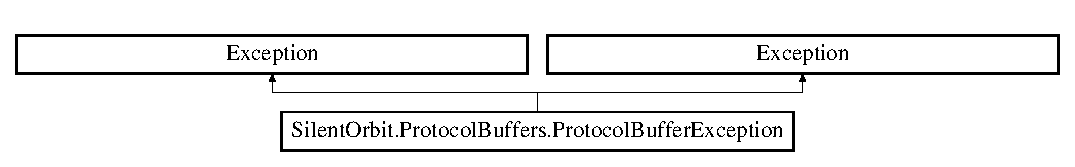
\includegraphics[height=1.794872cm]{class_silent_orbit_1_1_protocol_buffers_1_1_protocol_buffer_exception}
\end{center}
\end{figure}
\subsection*{Public Member Functions}
\begin{DoxyCompactItemize}
\item 
{\bfseries Protocol\+Buffer\+Exception} (string message)\hypertarget{class_silent_orbit_1_1_protocol_buffers_1_1_protocol_buffer_exception_a6028c070a3feff745b455ff61e9fd616}{}\label{class_silent_orbit_1_1_protocol_buffers_1_1_protocol_buffer_exception_a6028c070a3feff745b455ff61e9fd616}

\item 
{\bfseries Protocol\+Buffer\+Exception} (string message)\hypertarget{class_silent_orbit_1_1_protocol_buffers_1_1_protocol_buffer_exception_a6028c070a3feff745b455ff61e9fd616}{}\label{class_silent_orbit_1_1_protocol_buffers_1_1_protocol_buffer_exception_a6028c070a3feff745b455ff61e9fd616}

\end{DoxyCompactItemize}


\subsection{Detailed Description}
$>$ This exception is thrown when badly formatted protocol buffer data is read. /summary$>$ 

The documentation for this class was generated from the following file\+:\begin{DoxyCompactItemize}
\item 
/\+Users/\+Dat/\+Clion\+Projects/saas/cdti/\+C\+D\+T\+I\+Unity/\+Assets/scripts/Protocol\+Parser.\+cs\end{DoxyCompactItemize}

\hypertarget{class_json_1_1_reader}{}\section{Json\+:\+:Reader Class Reference}
\label{class_json_1_1_reader}\index{Json\+::\+Reader@{Json\+::\+Reader}}


Unserialize a \href{http://www.json.org}{\tt J\+S\+O\+N} document into a \hyperlink{class_json_1_1_value}{Value}.  




{\ttfamily \#include $<$json.\+h$>$}

\subsection*{Classes}
\begin{DoxyCompactItemize}
\item 
struct \hyperlink{struct_json_1_1_reader_1_1_structured_error}{Structured\+Error}
\begin{DoxyCompactList}\small\item\em An error tagged with where in the J\+S\+O\+N text it was encountered. \end{DoxyCompactList}\end{DoxyCompactItemize}
\subsection*{Public Types}
\begin{DoxyCompactItemize}
\item 
\hypertarget{class_json_1_1_reader_a3eec9118f3e9a672ba8348c3a79d0f45}{}typedef char {\bfseries Char}\label{class_json_1_1_reader_a3eec9118f3e9a672ba8348c3a79d0f45}

\item 
\hypertarget{class_json_1_1_reader_a46795b5b272bf79a7730e406cb96375a}{}typedef const Char $\ast$ {\bfseries Location}\label{class_json_1_1_reader_a46795b5b272bf79a7730e406cb96375a}

\end{DoxyCompactItemize}
\subsection*{Public Member Functions}
\begin{DoxyCompactItemize}
\item 
\hypertarget{class_json_1_1_reader_a0b3c4e24c8393354bab57a6ba3ffc27f}{}\hyperlink{class_json_1_1_reader_a0b3c4e24c8393354bab57a6ba3ffc27f}{Reader} ()\label{class_json_1_1_reader_a0b3c4e24c8393354bab57a6ba3ffc27f}

\begin{DoxyCompactList}\small\item\em Constructs a \hyperlink{class_json_1_1_reader}{Reader} allowing all features for parsing. \end{DoxyCompactList}\item 
\hypertarget{class_json_1_1_reader_a45f17831118337309180313e93ac33f8}{}\hyperlink{class_json_1_1_reader_a45f17831118337309180313e93ac33f8}{Reader} (const \hyperlink{class_json_1_1_features}{Features} \&features)\label{class_json_1_1_reader_a45f17831118337309180313e93ac33f8}

\begin{DoxyCompactList}\small\item\em Constructs a \hyperlink{class_json_1_1_reader}{Reader} allowing the specified feature set for parsing. \end{DoxyCompactList}\item 
bool \hyperlink{class_json_1_1_reader_af1da6c976ad1e96c742804c3853eef94}{parse} (const std\+::string \&document, \hyperlink{class_json_1_1_value}{Value} \&root, bool collect\+Comments=true)
\begin{DoxyCompactList}\small\item\em Read a \hyperlink{class_json_1_1_value}{Value} from a \href{http://www.json.org}{\tt J\+S\+O\+N} document. \end{DoxyCompactList}\item 
bool \hyperlink{class_json_1_1_reader_ac71ef2b64c7c27b062052e692af3fb32}{parse} (const char $\ast$begin\+Doc, const char $\ast$end\+Doc, \hyperlink{class_json_1_1_value}{Value} \&root, bool collect\+Comments=true)
\begin{DoxyCompactList}\small\item\em Read a \hyperlink{class_json_1_1_value}{Value} from a \href{http://www.json.org}{\tt J\+S\+O\+N} document. \end{DoxyCompactList}\item 
bool \hyperlink{class_json_1_1_reader_a8d0347e6b47343e4bc68be7ecdb9c4e9}{parse} (std\+::istream \&is, \hyperlink{class_json_1_1_value}{Value} \&root, bool collect\+Comments=true)
\begin{DoxyCompactList}\small\item\em Parse from input stream. \end{DoxyCompactList}\item 
std\+::string \hyperlink{class_json_1_1_reader_afa4a59e962d23c4d1c38b433fc95eefa}{get\+Formated\+Error\+Messages} () const 
\begin{DoxyCompactList}\small\item\em Returns a user friendly string that list errors in the parsed document. \end{DoxyCompactList}\item 
std\+::string \hyperlink{class_json_1_1_reader_a95ab50aa789132e9dee0fc1475c85acf}{get\+Formatted\+Error\+Messages} () const 
\begin{DoxyCompactList}\small\item\em Returns a user friendly string that list errors in the parsed document. \end{DoxyCompactList}\item 
std\+::vector$<$ \hyperlink{struct_json_1_1_reader_1_1_structured_error}{Structured\+Error} $>$ \hyperlink{class_json_1_1_reader_a08c2ea5ffc7d2a9c9e35020835624f0b}{get\+Structured\+Errors} () const 
\begin{DoxyCompactList}\small\item\em Returns a vector of structured erros encounted while parsing. \end{DoxyCompactList}\item 
bool \hyperlink{class_json_1_1_reader_ade6c28e0ef00d8f2e0aa2283f91c3e37}{push\+Error} (const \hyperlink{class_json_1_1_value}{Value} \&value, const std\+::string \&message)
\begin{DoxyCompactList}\small\item\em Add a semantic error message. \end{DoxyCompactList}\item 
bool \hyperlink{class_json_1_1_reader_a9b474233c3a7c688e340e70665d45223}{push\+Error} (const \hyperlink{class_json_1_1_value}{Value} \&value, const std\+::string \&message, const \hyperlink{class_json_1_1_value}{Value} \&extra)
\begin{DoxyCompactList}\small\item\em Add a semantic error message with extra context. \end{DoxyCompactList}\item 
bool \hyperlink{class_json_1_1_reader_a06b52dcc656549506b1ae6f05167ecf4}{good} () const 
\begin{DoxyCompactList}\small\item\em Return whether there are any errors. \end{DoxyCompactList}\end{DoxyCompactItemize}


\subsection{Detailed Description}
Unserialize a \href{http://www.json.org}{\tt J\+S\+O\+N} document into a \hyperlink{class_json_1_1_value}{Value}. 

\begin{DoxyRefDesc}{Deprecated}
\item[\hyperlink{deprecated__deprecated000005}{Deprecated}]Use \hyperlink{class_json_1_1_char_reader}{Char\+Reader} and \hyperlink{class_json_1_1_char_reader_builder}{Char\+Reader\+Builder}. \end{DoxyRefDesc}


\subsection{Member Function Documentation}
\hypertarget{class_json_1_1_reader_afa4a59e962d23c4d1c38b433fc95eefa}{}\index{Json\+::\+Reader@{Json\+::\+Reader}!get\+Formated\+Error\+Messages@{get\+Formated\+Error\+Messages}}
\index{get\+Formated\+Error\+Messages@{get\+Formated\+Error\+Messages}!Json\+::\+Reader@{Json\+::\+Reader}}
\subsubsection[{get\+Formated\+Error\+Messages}]{\setlength{\rightskip}{0pt plus 5cm}std\+::string Json\+::\+Reader\+::get\+Formated\+Error\+Messages (
\begin{DoxyParamCaption}
{}
\end{DoxyParamCaption}
) const}\label{class_json_1_1_reader_afa4a59e962d23c4d1c38b433fc95eefa}


Returns a user friendly string that list errors in the parsed document. 

\begin{DoxyReturn}{Returns}
Formatted error message with the list of errors with their location in the parsed document. An empty string is returned if no error occurred during parsing. 
\end{DoxyReturn}
\begin{DoxyRefDesc}{Deprecated}
\item[\hyperlink{deprecated__deprecated000006}{Deprecated}]Use \hyperlink{class_json_1_1_reader_a95ab50aa789132e9dee0fc1475c85acf}{get\+Formatted\+Error\+Messages()} instead (typo fix). \end{DoxyRefDesc}
\hypertarget{class_json_1_1_reader_a95ab50aa789132e9dee0fc1475c85acf}{}\index{Json\+::\+Reader@{Json\+::\+Reader}!get\+Formatted\+Error\+Messages@{get\+Formatted\+Error\+Messages}}
\index{get\+Formatted\+Error\+Messages@{get\+Formatted\+Error\+Messages}!Json\+::\+Reader@{Json\+::\+Reader}}
\subsubsection[{get\+Formatted\+Error\+Messages}]{\setlength{\rightskip}{0pt plus 5cm}std\+::string Json\+::\+Reader\+::get\+Formatted\+Error\+Messages (
\begin{DoxyParamCaption}
{}
\end{DoxyParamCaption}
) const}\label{class_json_1_1_reader_a95ab50aa789132e9dee0fc1475c85acf}


Returns a user friendly string that list errors in the parsed document. 

\begin{DoxyReturn}{Returns}
Formatted error message with the list of errors with their location in the parsed document. An empty string is returned if no error occurred during parsing. 
\end{DoxyReturn}
\hypertarget{class_json_1_1_reader_a08c2ea5ffc7d2a9c9e35020835624f0b}{}\index{Json\+::\+Reader@{Json\+::\+Reader}!get\+Structured\+Errors@{get\+Structured\+Errors}}
\index{get\+Structured\+Errors@{get\+Structured\+Errors}!Json\+::\+Reader@{Json\+::\+Reader}}
\subsubsection[{get\+Structured\+Errors}]{\setlength{\rightskip}{0pt plus 5cm}std\+::vector$<$ {\bf Reader\+::\+Structured\+Error} $>$ Json\+::\+Reader\+::get\+Structured\+Errors (
\begin{DoxyParamCaption}
{}
\end{DoxyParamCaption}
) const}\label{class_json_1_1_reader_a08c2ea5ffc7d2a9c9e35020835624f0b}


Returns a vector of structured erros encounted while parsing. 

\begin{DoxyReturn}{Returns}
A (possibly empty) vector of \hyperlink{struct_json_1_1_reader_1_1_structured_error}{Structured\+Error} objects. Currently only one error can be returned, but the caller should tolerate multiple errors. This can occur if the parser recovers from a non-\/fatal parse error and then encounters additional errors. 
\end{DoxyReturn}
\hypertarget{class_json_1_1_reader_a06b52dcc656549506b1ae6f05167ecf4}{}\index{Json\+::\+Reader@{Json\+::\+Reader}!good@{good}}
\index{good@{good}!Json\+::\+Reader@{Json\+::\+Reader}}
\subsubsection[{good}]{\setlength{\rightskip}{0pt plus 5cm}bool Json\+::\+Reader\+::good (
\begin{DoxyParamCaption}
{}
\end{DoxyParamCaption}
) const}\label{class_json_1_1_reader_a06b52dcc656549506b1ae6f05167ecf4}


Return whether there are any errors. 

\begin{DoxyReturn}{Returns}
{\ttfamily true} if there are no errors to report {\ttfamily false} if errors have occurred. 
\end{DoxyReturn}
\hypertarget{class_json_1_1_reader_af1da6c976ad1e96c742804c3853eef94}{}\index{Json\+::\+Reader@{Json\+::\+Reader}!parse@{parse}}
\index{parse@{parse}!Json\+::\+Reader@{Json\+::\+Reader}}
\subsubsection[{parse}]{\setlength{\rightskip}{0pt plus 5cm}bool Json\+::\+Reader\+::parse (
\begin{DoxyParamCaption}
\item[{const std\+::string \&}]{document, }
\item[{{\bf Value} \&}]{root, }
\item[{bool}]{collect\+Comments = {\ttfamily true}}
\end{DoxyParamCaption}
)}\label{class_json_1_1_reader_af1da6c976ad1e96c742804c3853eef94}


Read a \hyperlink{class_json_1_1_value}{Value} from a \href{http://www.json.org}{\tt J\+S\+O\+N} document. 


\begin{DoxyParams}{Parameters}
{\em document} & U\+T\+F-\/8 encoded string containing the document to read. \\
\hline
{\em root} & \mbox{[}out\mbox{]} Contains the root value of the document if it was successfully parsed. \\
\hline
{\em collect\+Comments} & {\ttfamily true} to collect comment and allow writing them back during serialization, {\ttfamily false} to discard comments. This parameter is ignored if \hyperlink{class_json_1_1_features_a33afd389719624b6bdb23950b3c346c9}{Features\+::allow\+Comments\+\_\+} is {\ttfamily false}. \\
\hline
\end{DoxyParams}
\begin{DoxyReturn}{Returns}
{\ttfamily true} if the document was successfully parsed, {\ttfamily false} if an error occurred. 
\end{DoxyReturn}
\hypertarget{class_json_1_1_reader_ac71ef2b64c7c27b062052e692af3fb32}{}\index{Json\+::\+Reader@{Json\+::\+Reader}!parse@{parse}}
\index{parse@{parse}!Json\+::\+Reader@{Json\+::\+Reader}}
\subsubsection[{parse}]{\setlength{\rightskip}{0pt plus 5cm}bool Json\+::\+Reader\+::parse (
\begin{DoxyParamCaption}
\item[{const char $\ast$}]{begin\+Doc, }
\item[{const char $\ast$}]{end\+Doc, }
\item[{{\bf Value} \&}]{root, }
\item[{bool}]{collect\+Comments = {\ttfamily true}}
\end{DoxyParamCaption}
)}\label{class_json_1_1_reader_ac71ef2b64c7c27b062052e692af3fb32}


Read a \hyperlink{class_json_1_1_value}{Value} from a \href{http://www.json.org}{\tt J\+S\+O\+N} document. 


\begin{DoxyParams}{Parameters}
{\em begin\+Doc} & Pointer on the beginning of the U\+T\+F-\/8 encoded string of the document to read. \\
\hline
{\em end\+Doc} & Pointer on the end of the U\+T\+F-\/8 encoded string of the document to read. Must be $>$= begin\+Doc. \\
\hline
{\em root} & \mbox{[}out\mbox{]} Contains the root value of the document if it was successfully parsed. \\
\hline
{\em collect\+Comments} & {\ttfamily true} to collect comment and allow writing them back during serialization, {\ttfamily false} to discard comments. This parameter is ignored if \hyperlink{class_json_1_1_features_a33afd389719624b6bdb23950b3c346c9}{Features\+::allow\+Comments\+\_\+} is {\ttfamily false}. \\
\hline
\end{DoxyParams}
\begin{DoxyReturn}{Returns}
{\ttfamily true} if the document was successfully parsed, {\ttfamily false} if an error occurred. 
\end{DoxyReturn}
\hypertarget{class_json_1_1_reader_a8d0347e6b47343e4bc68be7ecdb9c4e9}{}\index{Json\+::\+Reader@{Json\+::\+Reader}!parse@{parse}}
\index{parse@{parse}!Json\+::\+Reader@{Json\+::\+Reader}}
\subsubsection[{parse}]{\setlength{\rightskip}{0pt plus 5cm}bool Json\+::\+Reader\+::parse (
\begin{DoxyParamCaption}
\item[{std\+::istream \&}]{is, }
\item[{{\bf Value} \&}]{root, }
\item[{bool}]{collect\+Comments = {\ttfamily true}}
\end{DoxyParamCaption}
)}\label{class_json_1_1_reader_a8d0347e6b47343e4bc68be7ecdb9c4e9}


Parse from input stream. 

\begin{DoxySeeAlso}{See also}
\hyperlink{namespace_json_a4d245ef719cc0853e8e78eb5f99c16e5}{Json\+::operator$>$$>$(std\+::istream\&, Json\+::\+Value\&)}. 
\end{DoxySeeAlso}
\hypertarget{class_json_1_1_reader_ade6c28e0ef00d8f2e0aa2283f91c3e37}{}\index{Json\+::\+Reader@{Json\+::\+Reader}!push\+Error@{push\+Error}}
\index{push\+Error@{push\+Error}!Json\+::\+Reader@{Json\+::\+Reader}}
\subsubsection[{push\+Error}]{\setlength{\rightskip}{0pt plus 5cm}bool Json\+::\+Reader\+::push\+Error (
\begin{DoxyParamCaption}
\item[{const {\bf Value} \&}]{value, }
\item[{const std\+::string \&}]{message}
\end{DoxyParamCaption}
)}\label{class_json_1_1_reader_ade6c28e0ef00d8f2e0aa2283f91c3e37}


Add a semantic error message. 


\begin{DoxyParams}{Parameters}
{\em value} & J\+S\+O\+N \hyperlink{class_json_1_1_value}{Value} location associated with the error \\
\hline
{\em message} & The error message. \\
\hline
\end{DoxyParams}
\begin{DoxyReturn}{Returns}
{\ttfamily true} if the error was successfully added, {\ttfamily false} if the \hyperlink{class_json_1_1_value}{Value} offset exceeds the document size. 
\end{DoxyReturn}
\hypertarget{class_json_1_1_reader_a9b474233c3a7c688e340e70665d45223}{}\index{Json\+::\+Reader@{Json\+::\+Reader}!push\+Error@{push\+Error}}
\index{push\+Error@{push\+Error}!Json\+::\+Reader@{Json\+::\+Reader}}
\subsubsection[{push\+Error}]{\setlength{\rightskip}{0pt plus 5cm}bool Json\+::\+Reader\+::push\+Error (
\begin{DoxyParamCaption}
\item[{const {\bf Value} \&}]{value, }
\item[{const std\+::string \&}]{message, }
\item[{const {\bf Value} \&}]{extra}
\end{DoxyParamCaption}
)}\label{class_json_1_1_reader_a9b474233c3a7c688e340e70665d45223}


Add a semantic error message with extra context. 


\begin{DoxyParams}{Parameters}
{\em value} & J\+S\+O\+N \hyperlink{class_json_1_1_value}{Value} location associated with the error \\
\hline
{\em message} & The error message. \\
\hline
{\em extra} & Additional J\+S\+O\+N \hyperlink{class_json_1_1_value}{Value} location to contextualize the error \\
\hline
\end{DoxyParams}
\begin{DoxyReturn}{Returns}
{\ttfamily true} if the error was successfully added, {\ttfamily false} if either \hyperlink{class_json_1_1_value}{Value} offset exceeds the document size. 
\end{DoxyReturn}


The documentation for this class was generated from the following files\+:\begin{DoxyCompactItemize}
\item 
/home/fpoole/development/cpe406/saas/lib/jsoncpp/inc/json.\+h\item 
/home/fpoole/development/cpe406/saas/lib/jsoncpp/src/jsoncpp.\+cpp\end{DoxyCompactItemize}

\hypertarget{class_json_1_1_runtime_error}{}\section{Json\+:\+:Runtime\+Error Class Reference}
\label{class_json_1_1_runtime_error}\index{Json\+::\+Runtime\+Error@{Json\+::\+Runtime\+Error}}


{\ttfamily \#include $<$json.\+h$>$}

Inheritance diagram for Json\+:\+:Runtime\+Error\+:\begin{figure}[H]
\begin{center}
\leavevmode
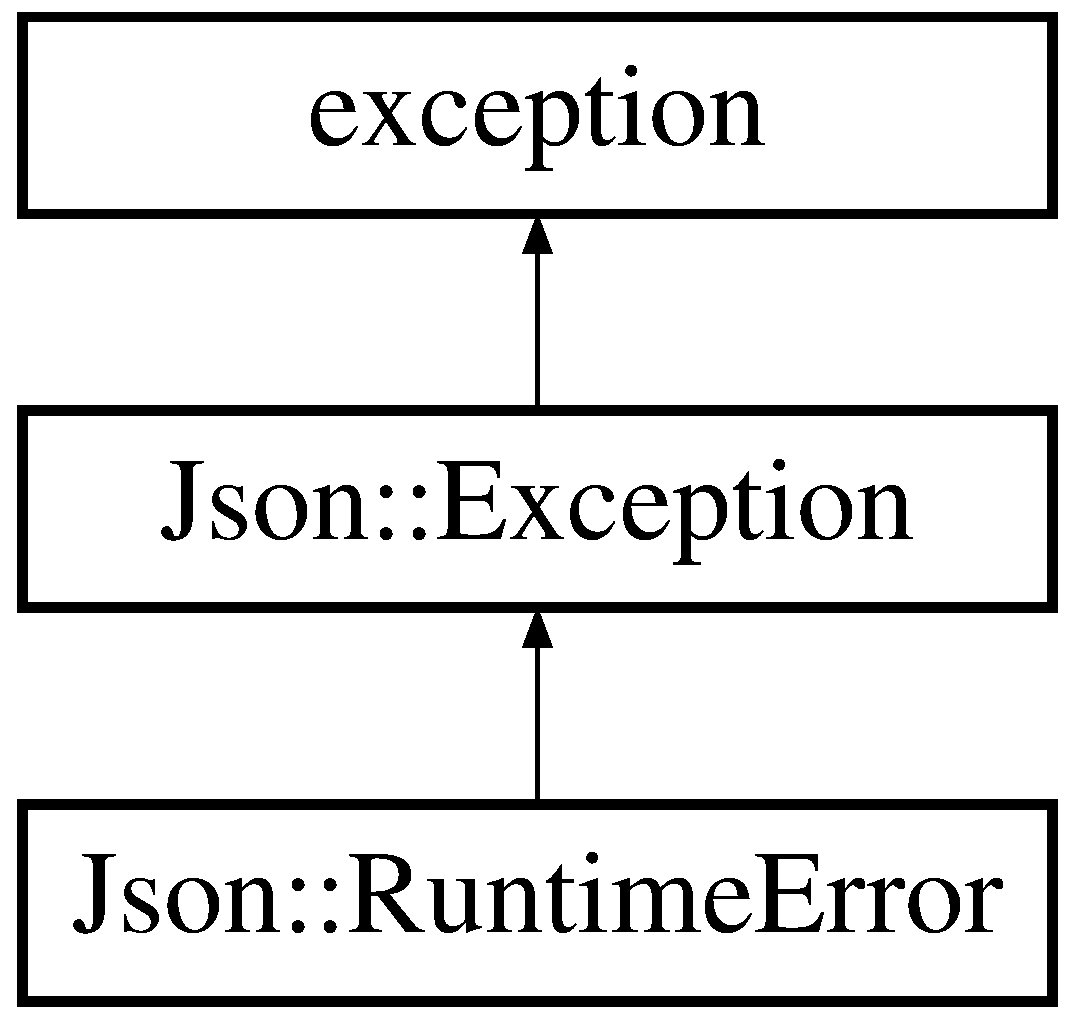
\includegraphics[height=3.000000cm]{class_json_1_1_runtime_error}
\end{center}
\end{figure}
\subsection*{Public Member Functions}
\begin{DoxyCompactItemize}
\item 
{\bfseries Runtime\+Error} (std\+::string const \&msg)\hypertarget{class_json_1_1_runtime_error_ae4f102d5c1efb773887efc8c7911e6f8}{}\label{class_json_1_1_runtime_error_ae4f102d5c1efb773887efc8c7911e6f8}

\end{DoxyCompactItemize}
\subsection*{Additional Inherited Members}


\subsection{Detailed Description}
Exceptions which the user cannot easily avoid.

E.\+g. out-\/of-\/memory (when we use malloc), stack-\/overflow, malicious input

\begin{DoxyRemark}{Remarks}
derived from \hyperlink{class_json_1_1_exception}{Json\+::\+Exception} 
\end{DoxyRemark}


The documentation for this class was generated from the following files\+:\begin{DoxyCompactItemize}
\item 
/home/andrea/\+Clion\+Projects/saas/lib/jsoncpp/inc/json.\+h\item 
/home/andrea/\+Clion\+Projects/saas/lib/jsoncpp/src/jsoncpp.\+cpp\end{DoxyCompactItemize}

\hypertarget{class_server_socket}{}\section{Server\+Socket Class Reference}
\label{class_server_socket}\index{Server\+Socket@{Server\+Socket}}


{\ttfamily \#include $<$Server\+Socket.\+h$>$}

Inheritance diagram for Server\+Socket\+:\begin{figure}[H]
\begin{center}
\leavevmode
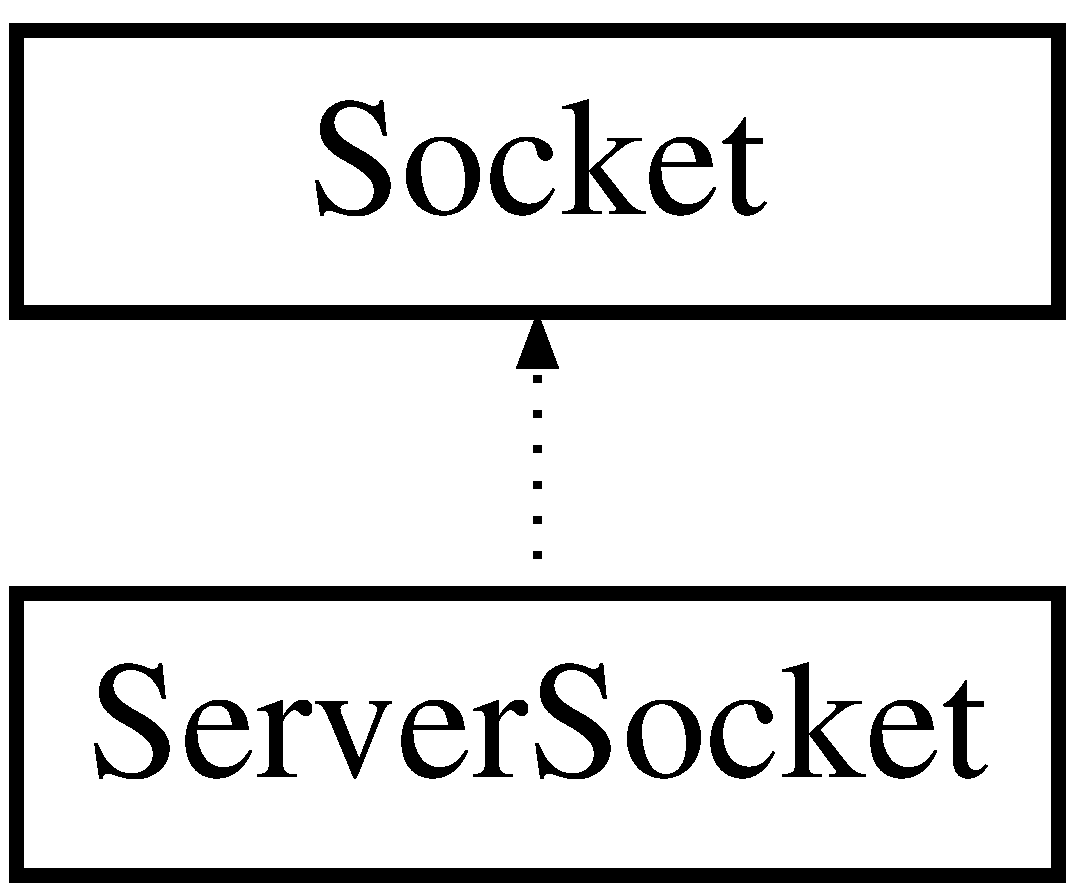
\includegraphics[height=2.000000cm]{class_server_socket}
\end{center}
\end{figure}
\subsection*{Public Member Functions}
\begin{DoxyCompactItemize}
\item 
\hyperlink{class_server_socket_a3b48c79e2e66bf8ab26b7350275b8ad0}{Server\+Socket} (const in\+\_\+port\+\_\+t port)
\item 
\hyperlink{class_server_socket_a2b3098589541243241ca25495155186c}{Server\+Socket} ()
\item 
virtual \hyperlink{class_server_socket_a510674d924c2544e6b0069e39c36516b}{$\sim$\+Server\+Socket} ()
\item 
const \hyperlink{class_server_socket}{Server\+Socket} \& \hyperlink{class_server_socket_ab5fe4b2d92d7014f7663c1bbacbbeda5}{operator$<$$<$} (const std\+::string \&) const 
\item 
const \hyperlink{class_server_socket}{Server\+Socket} \& \hyperlink{class_server_socket_a6bfabf01766bdb2c7f53274d8d771212}{operator$>$$>$} (std\+::string \&) const 
\item 
const \hyperlink{class_server_socket}{Server\+Socket} \& \hyperlink{class_server_socket_a184d1eff33380dd9708505429bfcbfb5}{operator$<$$<$} (const \+::google\+::protobuf\+::\+Message \&msg) const 
\item 
const \hyperlink{class_server_socket}{Server\+Socket} \& \hyperlink{class_server_socket_a5ff4a820f96e1a9dd5fa234ba3946f83}{operator$>$$>$} (\+::google\+::protobuf\+::\+Message \&msg) const 
\item 
void \hyperlink{class_server_socket_ae550e314a988575d05b1dec1c3c18020}{accept} (\hyperlink{class_server_socket}{Server\+Socket} \&)
\end{DoxyCompactItemize}


\subsection{Detailed Description}
A Server \hyperlink{class_socket}{Socket} is a socket used primarily by a server application, or whenever the socket expects to receive a connection, instead of connect to one. String data and protobuf data can be sent over the sockets. 

\subsection{Constructor \& Destructor Documentation}
\index{Server\+Socket@{Server\+Socket}!Server\+Socket@{Server\+Socket}}
\index{Server\+Socket@{Server\+Socket}!Server\+Socket@{Server\+Socket}}
\subsubsection[{\texorpdfstring{Server\+Socket(const in\+\_\+port\+\_\+t port)}{ServerSocket(const in_port_t port)}}]{\setlength{\rightskip}{0pt plus 5cm}Server\+Socket\+::\+Server\+Socket (
\begin{DoxyParamCaption}
\item[{const in\+\_\+port\+\_\+t}]{port}
\end{DoxyParamCaption}
)}\hypertarget{class_server_socket_a3b48c79e2e66bf8ab26b7350275b8ad0}{}\label{class_server_socket_a3b48c79e2e66bf8ab26b7350275b8ad0}
Create and open a socket on the specified port. 
\begin{DoxyParams}{Parameters}
{\em port} & the port number \\
\hline
\end{DoxyParams}
\index{Server\+Socket@{Server\+Socket}!Server\+Socket@{Server\+Socket}}
\index{Server\+Socket@{Server\+Socket}!Server\+Socket@{Server\+Socket}}
\subsubsection[{\texorpdfstring{Server\+Socket()}{ServerSocket()}}]{\setlength{\rightskip}{0pt plus 5cm}Server\+Socket\+::\+Server\+Socket (
\begin{DoxyParamCaption}
{}
\end{DoxyParamCaption}
)\hspace{0.3cm}{\ttfamily [inline]}}\hypertarget{class_server_socket_a2b3098589541243241ca25495155186c}{}\label{class_server_socket_a2b3098589541243241ca25495155186c}
Create a socket for accepting a current connection. \index{Server\+Socket@{Server\+Socket}!````~Server\+Socket@{$\sim$\+Server\+Socket}}
\index{````~Server\+Socket@{$\sim$\+Server\+Socket}!Server\+Socket@{Server\+Socket}}
\subsubsection[{\texorpdfstring{$\sim$\+Server\+Socket()}{~ServerSocket()}}]{\setlength{\rightskip}{0pt plus 5cm}Server\+Socket\+::$\sim$\+Server\+Socket (
\begin{DoxyParamCaption}
{}
\end{DoxyParamCaption}
)\hspace{0.3cm}{\ttfamily [virtual]}}\hypertarget{class_server_socket_a510674d924c2544e6b0069e39c36516b}{}\label{class_server_socket_a510674d924c2544e6b0069e39c36516b}
Close the socket. 

\subsection{Member Function Documentation}
\index{Server\+Socket@{Server\+Socket}!accept@{accept}}
\index{accept@{accept}!Server\+Socket@{Server\+Socket}}
\subsubsection[{\texorpdfstring{accept(\+Server\+Socket \&)}{accept(ServerSocket &)}}]{\setlength{\rightskip}{0pt plus 5cm}void Server\+Socket\+::accept (
\begin{DoxyParamCaption}
\item[{{\bf Server\+Socket} \&}]{sock}
\end{DoxyParamCaption}
)}\hypertarget{class_server_socket_ae550e314a988575d05b1dec1c3c18020}{}\label{class_server_socket_ae550e314a988575d05b1dec1c3c18020}
Accept a connection and bind it to the new socket. \index{Server\+Socket@{Server\+Socket}!operator$<$$<$@{operator$<$$<$}}
\index{operator$<$$<$@{operator$<$$<$}!Server\+Socket@{Server\+Socket}}
\subsubsection[{\texorpdfstring{operator$<$$<$(const std\+::string \&) const }{operator<<(const std::string &) const }}]{\setlength{\rightskip}{0pt plus 5cm}const {\bf Server\+Socket} \& Server\+Socket\+::operator$<$$<$ (
\begin{DoxyParamCaption}
\item[{const std\+::string \&}]{s}
\end{DoxyParamCaption}
) const}\hypertarget{class_server_socket_ab5fe4b2d92d7014f7663c1bbacbbeda5}{}\label{class_server_socket_ab5fe4b2d92d7014f7663c1bbacbbeda5}
Write a string to the client. string the string to write \index{Server\+Socket@{Server\+Socket}!operator$<$$<$@{operator$<$$<$}}
\index{operator$<$$<$@{operator$<$$<$}!Server\+Socket@{Server\+Socket}}
\subsubsection[{\texorpdfstring{operator$<$$<$(const \+::google\+::protobuf\+::\+Message \&msg) const }{operator<<(const ::google::protobuf::Message &msg) const }}]{\setlength{\rightskip}{0pt plus 5cm}const {\bf Server\+Socket} \& Server\+Socket\+::operator$<$$<$ (
\begin{DoxyParamCaption}
\item[{const \+::google\+::protobuf\+::\+Message \&}]{msg}
\end{DoxyParamCaption}
) const}\hypertarget{class_server_socket_a184d1eff33380dd9708505429bfcbfb5}{}\label{class_server_socket_a184d1eff33380dd9708505429bfcbfb5}
Write a protocol buffer to the client. msg the protocol buffer message to write \index{Server\+Socket@{Server\+Socket}!operator$>$$>$@{operator$>$$>$}}
\index{operator$>$$>$@{operator$>$$>$}!Server\+Socket@{Server\+Socket}}
\subsubsection[{\texorpdfstring{operator$>$$>$(std\+::string \&) const }{operator>>(std::string &) const }}]{\setlength{\rightskip}{0pt plus 5cm}const {\bf Server\+Socket} \& Server\+Socket\+::operator$>$$>$ (
\begin{DoxyParamCaption}
\item[{std\+::string \&}]{s}
\end{DoxyParamCaption}
) const}\hypertarget{class_server_socket_a6bfabf01766bdb2c7f53274d8d771212}{}\label{class_server_socket_a6bfabf01766bdb2c7f53274d8d771212}
Read a string form the client. string the string to read into \index{Server\+Socket@{Server\+Socket}!operator$>$$>$@{operator$>$$>$}}
\index{operator$>$$>$@{operator$>$$>$}!Server\+Socket@{Server\+Socket}}
\subsubsection[{\texorpdfstring{operator$>$$>$(\+::google\+::protobuf\+::\+Message \&msg) const }{operator>>(::google::protobuf::Message &msg) const }}]{\setlength{\rightskip}{0pt plus 5cm}const {\bf Server\+Socket} \& Server\+Socket\+::operator$>$$>$ (
\begin{DoxyParamCaption}
\item[{\+::google\+::protobuf\+::\+Message \&}]{msg}
\end{DoxyParamCaption}
) const}\hypertarget{class_server_socket_a5ff4a820f96e1a9dd5fa234ba3946f83}{}\label{class_server_socket_a5ff4a820f96e1a9dd5fa234ba3946f83}
Read a protocol buffer from the client into message. msg the protocol buffer message to read into 

The documentation for this class was generated from the following files\+:\begin{DoxyCompactItemize}
\item 
/\+Users/\+Dat/\+Clion\+Projects/saas/lib/network/inc/Server\+Socket.\+h\item 
/\+Users/\+Dat/\+Clion\+Projects/saas/lib/network/src/Server\+Socket.\+cpp\end{DoxyCompactItemize}

\hypertarget{class_simulation_flights_i_o}{}\section{Simulation\+Flights\+I\+O Class Reference}
\label{class_simulation_flights_i_o}\index{Simulation\+Flights\+I\+O@{Simulation\+Flights\+I\+O}}
Inheritance diagram for Simulation\+Flights\+I\+O\+:\begin{figure}[H]
\begin{center}
\leavevmode
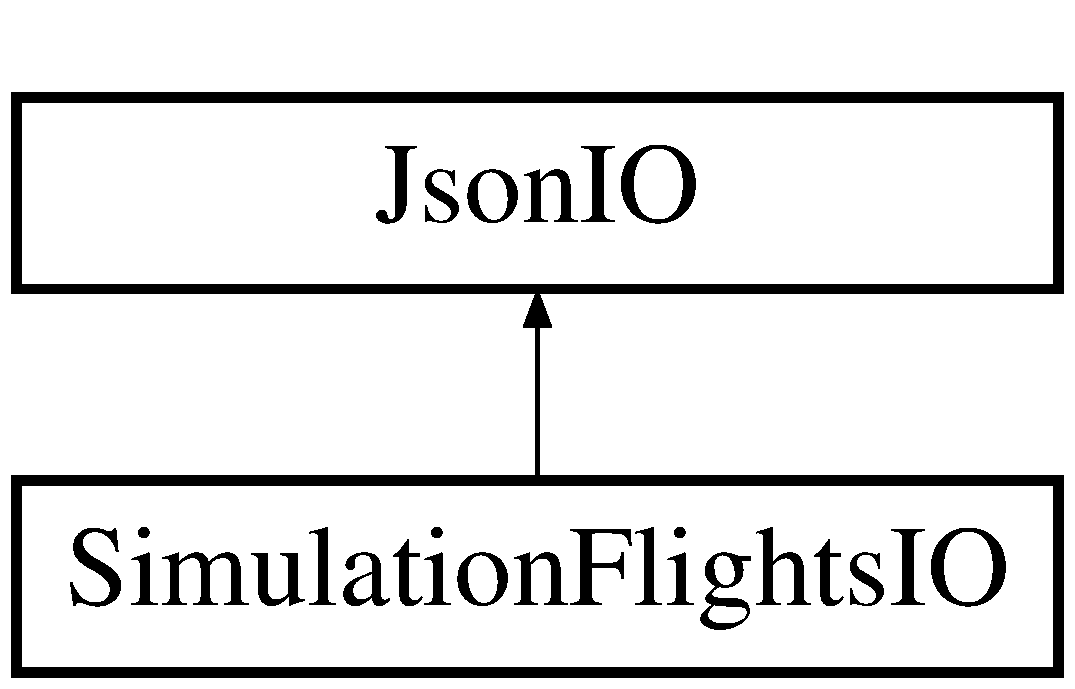
\includegraphics[height=2.000000cm]{class_simulation_flights_i_o}
\end{center}
\end{figure}
\subsection*{Public Member Functions}
\begin{DoxyCompactItemize}
\item 
\hypertarget{class_simulation_flights_i_o_aab1dd1c43b626e70bc60d4b79d703597}{}virtual void {\bfseries write\+File} (\hyperlink{class_json_1_1_value}{Json\+::\+Value} value)\label{class_simulation_flights_i_o_aab1dd1c43b626e70bc60d4b79d703597}

\end{DoxyCompactItemize}
\subsection*{Static Public Member Functions}
\begin{DoxyCompactItemize}
\item 
\hypertarget{class_simulation_flights_i_o_a4403f368173eeaf850e4d161e00d064f}{}static \hyperlink{class_json_1_1_value}{Json\+::\+Value} {\bfseries Read\+File} ()\label{class_simulation_flights_i_o_a4403f368173eeaf850e4d161e00d064f}

\item 
\hypertarget{class_simulation_flights_i_o_a0fecd6176618527ce882c1bd705cea2e}{}static \hyperlink{class_json_1_1_value}{Json\+::\+Value} {\bfseries Get\+Simulation\+Flights} ()\label{class_simulation_flights_i_o_a0fecd6176618527ce882c1bd705cea2e}

\item 
\hypertarget{class_simulation_flights_i_o_ab80deb0dbd2eff210c5a24211fbb0319}{}static std\+::vector$<$ \hyperlink{class_json_1_1_value}{Json\+::\+Value} $>$ {\bfseries Get\+All\+A\+D\+S\+B\+Reports} ()\label{class_simulation_flights_i_o_ab80deb0dbd2eff210c5a24211fbb0319}

\item 
\hypertarget{class_simulation_flights_i_o_ac54cf3a5ddcda61e56fbf523cfe7c541}{}static std\+::vector$<$ \hyperlink{class_json_1_1_value}{Json\+::\+Value} $>$ {\bfseries Get\+All\+T\+C\+A\+S\+Reports} ()\label{class_simulation_flights_i_o_ac54cf3a5ddcda61e56fbf523cfe7c541}

\item 
\hypertarget{class_simulation_flights_i_o_aec11fa10f5610c6505c0ffe8c59ded5b}{}static std\+::vector$<$ \hyperlink{class_json_1_1_value}{Json\+::\+Value} $>$ {\bfseries Get\+All\+Radar\+Reports} ()\label{class_simulation_flights_i_o_aec11fa10f5610c6505c0ffe8c59ded5b}

\item 
\hypertarget{class_simulation_flights_i_o_a047aa637503e4988f9b9c0da284a601b}{}static std\+::vector$<$ \hyperlink{class_json_1_1_value}{Json\+::\+Value} $>$ {\bfseries Get\+A\+Ll\+Ownship\+Reports} ()\label{class_simulation_flights_i_o_a047aa637503e4988f9b9c0da284a601b}

\end{DoxyCompactItemize}


The documentation for this class was generated from the following files\+:\begin{DoxyCompactItemize}
\item 
/home/frank/dev/cpe402/saas/lib/jsonio/inc/Simulation\+Flights\+I\+O.\+h\item 
/home/frank/dev/cpe402/saas/lib/jsonio/src/Simulation\+Flights\+I\+O.\+cpp\end{DoxyCompactItemize}

\hypertarget{class_simulation_report}{}\section{Simulation\+Report Class Reference}
\label{class_simulation_report}\index{Simulation\+Report@{Simulation\+Report}}
\subsection*{Public Member Functions}
\begin{DoxyCompactItemize}
\item 
\hyperlink{class_simulation_report_af1a596c7f3f123d5b174124123eaed04}{Simulation\+Report} ()
\item 
Ownship\+Report \hyperlink{class_simulation_report_a75ee5df9afd639a9fa8223d587d3cc35}{get\+Next\+Ownship\+Report} ()
\item 
Tcas\+Report \hyperlink{class_simulation_report_a8496265382424b82207b98122c872262}{get\+Next\+Tcas\+Report} ()
\item 
Radar\+Report \hyperlink{class_simulation_report_aa83b2ee8f95f9149b5f26ab11f84cfc8}{get\+Next\+Radar\+Report} ()
\item 
Ads\+B\+Report \hyperlink{class_simulation_report_a2762e819b3d3210ebcdc8716addb3eab}{get\+Next\+Adsb\+Report} ()
\item 
bool \hyperlink{class_simulation_report_a1a9d80360b8e5ebd3c487c487b44a1ec}{has\+Next\+Ownship\+Report} ()
\item 
bool \hyperlink{class_simulation_report_a749c031cf1da6d596c02d4787246f3de}{has\+Next\+Tcas\+Report} ()
\item 
bool \hyperlink{class_simulation_report_aae24d4ab4d5b5b3ff5802d9a571cd9c4}{has\+Next\+Radar\+Report} ()
\item 
bool \hyperlink{class_simulation_report_aecdc89ccb21ff03828d5724e59ded0ea}{has\+Next\+Adsb\+Report} ()
\end{DoxyCompactItemize}


\subsection{Constructor \& Destructor Documentation}
\index{Simulation\+Report@{Simulation\+Report}!Simulation\+Report@{Simulation\+Report}}
\index{Simulation\+Report@{Simulation\+Report}!Simulation\+Report@{Simulation\+Report}}
\subsubsection[{\texorpdfstring{Simulation\+Report()}{SimulationReport()}}]{\setlength{\rightskip}{0pt plus 5cm}Simulation\+Report\+::\+Simulation\+Report (
\begin{DoxyParamCaption}
{}
\end{DoxyParamCaption}
)}\hypertarget{class_simulation_report_af1a596c7f3f123d5b174124123eaed04}{}\label{class_simulation_report_af1a596c7f3f123d5b174124123eaed04}
Constructor for a \hyperlink{class_simulation_report}{Simulation\+Report} 

\subsection{Member Function Documentation}
\index{Simulation\+Report@{Simulation\+Report}!get\+Next\+Adsb\+Report@{get\+Next\+Adsb\+Report}}
\index{get\+Next\+Adsb\+Report@{get\+Next\+Adsb\+Report}!Simulation\+Report@{Simulation\+Report}}
\subsubsection[{\texorpdfstring{get\+Next\+Adsb\+Report()}{getNextAdsbReport()}}]{\setlength{\rightskip}{0pt plus 5cm}Ads\+B\+Report Simulation\+Report\+::get\+Next\+Adsb\+Report (
\begin{DoxyParamCaption}
{}
\end{DoxyParamCaption}
)}\hypertarget{class_simulation_report_a2762e819b3d3210ebcdc8716addb3eab}{}\label{class_simulation_report_a2762e819b3d3210ebcdc8716addb3eab}
Finds and returns the next Adsb\+Report from the iterator. \begin{DoxyReturn}{Returns}
Ads\+B\+Report with the data from the sensor. 
\end{DoxyReturn}
\index{Simulation\+Report@{Simulation\+Report}!get\+Next\+Ownship\+Report@{get\+Next\+Ownship\+Report}}
\index{get\+Next\+Ownship\+Report@{get\+Next\+Ownship\+Report}!Simulation\+Report@{Simulation\+Report}}
\subsubsection[{\texorpdfstring{get\+Next\+Ownship\+Report()}{getNextOwnshipReport()}}]{\setlength{\rightskip}{0pt plus 5cm}Ownship\+Report Simulation\+Report\+::get\+Next\+Ownship\+Report (
\begin{DoxyParamCaption}
{}
\end{DoxyParamCaption}
)}\hypertarget{class_simulation_report_a75ee5df9afd639a9fa8223d587d3cc35}{}\label{class_simulation_report_a75ee5df9afd639a9fa8223d587d3cc35}
Finds and returns the next Ownship\+Report from an iterator \begin{DoxyReturn}{Returns}
Ownship\+Report the next report 
\end{DoxyReturn}
\index{Simulation\+Report@{Simulation\+Report}!get\+Next\+Radar\+Report@{get\+Next\+Radar\+Report}}
\index{get\+Next\+Radar\+Report@{get\+Next\+Radar\+Report}!Simulation\+Report@{Simulation\+Report}}
\subsubsection[{\texorpdfstring{get\+Next\+Radar\+Report()}{getNextRadarReport()}}]{\setlength{\rightskip}{0pt plus 5cm}Radar\+Report Simulation\+Report\+::get\+Next\+Radar\+Report (
\begin{DoxyParamCaption}
{}
\end{DoxyParamCaption}
)}\hypertarget{class_simulation_report_aa83b2ee8f95f9149b5f26ab11f84cfc8}{}\label{class_simulation_report_aa83b2ee8f95f9149b5f26ab11f84cfc8}
Finds and returns the next Radar\+Report from the iterator \begin{DoxyReturn}{Returns}
Radar\+Report with the data from the sensor. 
\end{DoxyReturn}
\index{Simulation\+Report@{Simulation\+Report}!get\+Next\+Tcas\+Report@{get\+Next\+Tcas\+Report}}
\index{get\+Next\+Tcas\+Report@{get\+Next\+Tcas\+Report}!Simulation\+Report@{Simulation\+Report}}
\subsubsection[{\texorpdfstring{get\+Next\+Tcas\+Report()}{getNextTcasReport()}}]{\setlength{\rightskip}{0pt plus 5cm}Tcas\+Report Simulation\+Report\+::get\+Next\+Tcas\+Report (
\begin{DoxyParamCaption}
{}
\end{DoxyParamCaption}
)}\hypertarget{class_simulation_report_a8496265382424b82207b98122c872262}{}\label{class_simulation_report_a8496265382424b82207b98122c872262}
Finds and returns the next Tcas\+Report from an iterator \begin{DoxyReturn}{Returns}
Tcas\+Report with the data from the sensor. 
\end{DoxyReturn}
\index{Simulation\+Report@{Simulation\+Report}!has\+Next\+Adsb\+Report@{has\+Next\+Adsb\+Report}}
\index{has\+Next\+Adsb\+Report@{has\+Next\+Adsb\+Report}!Simulation\+Report@{Simulation\+Report}}
\subsubsection[{\texorpdfstring{has\+Next\+Adsb\+Report()}{hasNextAdsbReport()}}]{\setlength{\rightskip}{0pt plus 5cm}bool Simulation\+Report\+::has\+Next\+Adsb\+Report (
\begin{DoxyParamCaption}
{}
\end{DoxyParamCaption}
)}\hypertarget{class_simulation_report_aecdc89ccb21ff03828d5724e59ded0ea}{}\label{class_simulation_report_aecdc89ccb21ff03828d5724e59ded0ea}
Verifies if there are any more Adsb\+Reports left. \begin{DoxyReturn}{Returns}
true if there are any more Adsb\+Reports in the vector. 
\end{DoxyReturn}
\index{Simulation\+Report@{Simulation\+Report}!has\+Next\+Ownship\+Report@{has\+Next\+Ownship\+Report}}
\index{has\+Next\+Ownship\+Report@{has\+Next\+Ownship\+Report}!Simulation\+Report@{Simulation\+Report}}
\subsubsection[{\texorpdfstring{has\+Next\+Ownship\+Report()}{hasNextOwnshipReport()}}]{\setlength{\rightskip}{0pt plus 5cm}bool Simulation\+Report\+::has\+Next\+Ownship\+Report (
\begin{DoxyParamCaption}
{}
\end{DoxyParamCaption}
)}\hypertarget{class_simulation_report_a1a9d80360b8e5ebd3c487c487b44a1ec}{}\label{class_simulation_report_a1a9d80360b8e5ebd3c487c487b44a1ec}
Verifies if there are any more Ownship\+Reports left. \begin{DoxyReturn}{Returns}
true if there are any more Ownship\+Reports in the vector. 
\end{DoxyReturn}
\index{Simulation\+Report@{Simulation\+Report}!has\+Next\+Radar\+Report@{has\+Next\+Radar\+Report}}
\index{has\+Next\+Radar\+Report@{has\+Next\+Radar\+Report}!Simulation\+Report@{Simulation\+Report}}
\subsubsection[{\texorpdfstring{has\+Next\+Radar\+Report()}{hasNextRadarReport()}}]{\setlength{\rightskip}{0pt plus 5cm}bool Simulation\+Report\+::has\+Next\+Radar\+Report (
\begin{DoxyParamCaption}
{}
\end{DoxyParamCaption}
)}\hypertarget{class_simulation_report_aae24d4ab4d5b5b3ff5802d9a571cd9c4}{}\label{class_simulation_report_aae24d4ab4d5b5b3ff5802d9a571cd9c4}
Verifies if there are any more Radar\+Reports left. \begin{DoxyReturn}{Returns}
true if there are any more Radar\+Reports in the vector. 
\end{DoxyReturn}
\index{Simulation\+Report@{Simulation\+Report}!has\+Next\+Tcas\+Report@{has\+Next\+Tcas\+Report}}
\index{has\+Next\+Tcas\+Report@{has\+Next\+Tcas\+Report}!Simulation\+Report@{Simulation\+Report}}
\subsubsection[{\texorpdfstring{has\+Next\+Tcas\+Report()}{hasNextTcasReport()}}]{\setlength{\rightskip}{0pt plus 5cm}bool Simulation\+Report\+::has\+Next\+Tcas\+Report (
\begin{DoxyParamCaption}
{}
\end{DoxyParamCaption}
)}\hypertarget{class_simulation_report_a749c031cf1da6d596c02d4787246f3de}{}\label{class_simulation_report_a749c031cf1da6d596c02d4787246f3de}
Verifies if there are any more Tcas\+Reports left. \begin{DoxyReturn}{Returns}
true if there are any more Tcas\+Reports in the vector. 
\end{DoxyReturn}


The documentation for this class was generated from the following files\+:\begin{DoxyCompactItemize}
\item 
/home/andrea/\+Clion\+Projects/saas/saap/app/Simulation\+Report.\+h\item 
/home/andrea/\+Clion\+Projects/saas/saap/app/Simulation\+Report.\+cpp\end{DoxyCompactItemize}

\input{struct_snapshot}
\hypertarget{class_socket}{}\section{Socket Class Reference}
\label{class_socket}\index{Socket@{Socket}}


{\ttfamily \#include $<$Socket.\+h$>$}

Inheritance diagram for Socket\+:\begin{figure}[H]
\begin{center}
\leavevmode
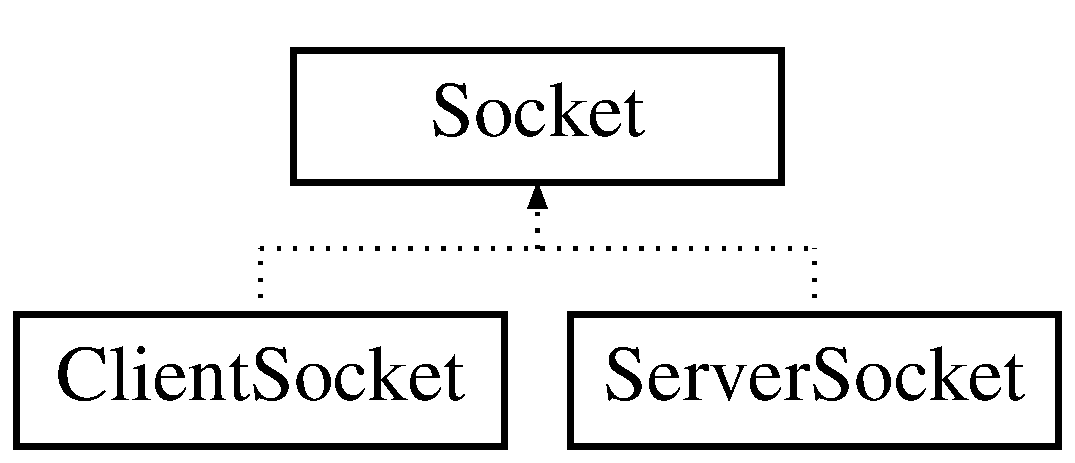
\includegraphics[height=2.000000cm]{class_socket}
\end{center}
\end{figure}
\subsection*{Public Member Functions}
\begin{DoxyCompactItemize}
\item 
bool \hyperlink{class_socket_a8aa4d2a7c1a49186f214d0387c553661}{Create} ()
\item 
bool \hyperlink{class_socket_ae0cf2d7a389fbd76f96517e8db9b2ed9}{Bind} (const in\+\_\+port\+\_\+t port)
\item 
bool \hyperlink{class_socket_ac743519b14d7b964ee85927215fb266d}{Listen} () const 
\item 
bool \hyperlink{class_socket_a8917c07b7c30249cb2347f45a0285793}{Accept} (\hyperlink{class_socket}{Socket} \&new\+\_\+socket) const 
\item 
bool \hyperlink{class_socket_a9561a87ddb6f9014a2dbc95b6326db03}{Connect} (const std\+::string host, const in\+\_\+port\+\_\+t port)
\item 
bool \hyperlink{class_socket_af20012023497dcccdfbce6eb6341a487}{Send} (const std\+::string \&msg) const 
\item 
bool \hyperlink{class_socket_aa57655f2829ba63a44d6b2e026292bd9}{Send} (const void $\ast$msg, size\+\_\+t len) const 
\item 
size\+\_\+t \hyperlink{class_socket_a3f11ff7aecfbe902d5dc0ef6055e04bb}{Recv} (std\+::string \&bfr, int flags=0) const 
\item 
size\+\_\+t \hyperlink{class_socket_ab0220973615a4a87b26e9b34148ccfad}{Recv} (void $\ast$bfr, size\+\_\+t len, int flags=0) const 
\item 
bool \hyperlink{class_socket_a0e3b60b515ad57286079cfd502fa4edd}{Set\+Non\+Blocking} (const bool is\+\_\+non\+\_\+blocking)
\item 
bool \hyperlink{class_socket_af614b429b6f26fa191de2c26fdc188d4}{Is\+Valid} () const 
\end{DoxyCompactItemize}


\subsection{Detailed Description}
A \hyperlink{class_socket}{Socket} is a logical endpoint for communications that exists on the transport layer. The \hyperlink{class_socket}{Socket} class includes functions for initializing connections with other hosts and sending and receiving data. 

\subsection{Member Function Documentation}
\hypertarget{class_socket_a8917c07b7c30249cb2347f45a0285793}{}\index{Socket@{Socket}!Accept@{Accept}}
\index{Accept@{Accept}!Socket@{Socket}}
\subsubsection[{Accept}]{\setlength{\rightskip}{0pt plus 5cm}bool Socket\+::\+Accept (
\begin{DoxyParamCaption}
\item[{{\bf Socket} \&}]{new\+\_\+socket}
\end{DoxyParamCaption}
) const}\label{class_socket_a8917c07b7c30249cb2347f45a0285793}
Accept a socket connection and bind the socket. \begin{DoxyReturn}{Returns}
true if no errors occurred 
\end{DoxyReturn}
\hypertarget{class_socket_ae0cf2d7a389fbd76f96517e8db9b2ed9}{}\index{Socket@{Socket}!Bind@{Bind}}
\index{Bind@{Bind}!Socket@{Socket}}
\subsubsection[{Bind}]{\setlength{\rightskip}{0pt plus 5cm}bool Socket\+::\+Bind (
\begin{DoxyParamCaption}
\item[{const in\+\_\+port\+\_\+t}]{port}
\end{DoxyParamCaption}
)}\label{class_socket_ae0cf2d7a389fbd76f96517e8db9b2ed9}
Bind a socket to a port. 
\begin{DoxyParams}{Parameters}
{\em port} & the port to bind the socket to \\
\hline
\end{DoxyParams}
\begin{DoxyReturn}{Returns}
true if no errors occurred 
\end{DoxyReturn}
\hypertarget{class_socket_a9561a87ddb6f9014a2dbc95b6326db03}{}\index{Socket@{Socket}!Connect@{Connect}}
\index{Connect@{Connect}!Socket@{Socket}}
\subsubsection[{Connect}]{\setlength{\rightskip}{0pt plus 5cm}bool Socket\+::\+Connect (
\begin{DoxyParamCaption}
\item[{const std\+::string}]{host, }
\item[{const in\+\_\+port\+\_\+t}]{port}
\end{DoxyParamCaption}
)}\label{class_socket_a9561a87ddb6f9014a2dbc95b6326db03}
Connect to a socket. 
\begin{DoxyParams}{Parameters}
{\em host} & the host to connect to \\
\hline
{\em port} & the port to connect to \\
\hline
\end{DoxyParams}
\begin{DoxyReturn}{Returns}
true if connection was successful 
\end{DoxyReturn}
\hypertarget{class_socket_a8aa4d2a7c1a49186f214d0387c553661}{}\index{Socket@{Socket}!Create@{Create}}
\index{Create@{Create}!Socket@{Socket}}
\subsubsection[{Create}]{\setlength{\rightskip}{0pt plus 5cm}bool Socket\+::\+Create (
\begin{DoxyParamCaption}
{}
\end{DoxyParamCaption}
)}\label{class_socket_a8aa4d2a7c1a49186f214d0387c553661}
Create a new socket. \begin{DoxyReturn}{Returns}
true if no errors occurred 
\end{DoxyReturn}
\hypertarget{class_socket_af614b429b6f26fa191de2c26fdc188d4}{}\index{Socket@{Socket}!Is\+Valid@{Is\+Valid}}
\index{Is\+Valid@{Is\+Valid}!Socket@{Socket}}
\subsubsection[{Is\+Valid}]{\setlength{\rightskip}{0pt plus 5cm}bool Socket\+::\+Is\+Valid (
\begin{DoxyParamCaption}
{}
\end{DoxyParamCaption}
) const\hspace{0.3cm}{\ttfamily [inline]}}\label{class_socket_af614b429b6f26fa191de2c26fdc188d4}
Check of the socket is valid for use. \begin{DoxyReturn}{Returns}
true if the socket is valid for use or return false if the socket has not been created 
\end{DoxyReturn}
\hypertarget{class_socket_ac743519b14d7b964ee85927215fb266d}{}\index{Socket@{Socket}!Listen@{Listen}}
\index{Listen@{Listen}!Socket@{Socket}}
\subsubsection[{Listen}]{\setlength{\rightskip}{0pt plus 5cm}bool Socket\+::\+Listen (
\begin{DoxyParamCaption}
{}
\end{DoxyParamCaption}
) const}\label{class_socket_ac743519b14d7b964ee85927215fb266d}
Listen for incoming network connections. \begin{DoxyReturn}{Returns}
true if no errors occurred 
\end{DoxyReturn}
\hypertarget{class_socket_a3f11ff7aecfbe902d5dc0ef6055e04bb}{}\index{Socket@{Socket}!Recv@{Recv}}
\index{Recv@{Recv}!Socket@{Socket}}
\subsubsection[{Recv}]{\setlength{\rightskip}{0pt plus 5cm}size\+\_\+t Socket\+::\+Recv (
\begin{DoxyParamCaption}
\item[{std\+::string \&}]{bfr, }
\item[{int}]{flags = {\ttfamily 0}}
\end{DoxyParamCaption}
) const}\label{class_socket_a3f11ff7aecfbe902d5dc0ef6055e04bb}
Receive string data from the socket (Default, 500 bytes). 
\begin{DoxyParams}{Parameters}
{\em bfr} & the string to write to \\
\hline
{\em flags} & flags for socket reading options \\
\hline
\end{DoxyParams}
\begin{DoxyReturn}{Returns}
the number of bytes read 
\end{DoxyReturn}
\hypertarget{class_socket_ab0220973615a4a87b26e9b34148ccfad}{}\index{Socket@{Socket}!Recv@{Recv}}
\index{Recv@{Recv}!Socket@{Socket}}
\subsubsection[{Recv}]{\setlength{\rightskip}{0pt plus 5cm}size\+\_\+t Socket\+::\+Recv (
\begin{DoxyParamCaption}
\item[{void $\ast$}]{bfr, }
\item[{size\+\_\+t}]{len, }
\item[{int}]{flags = {\ttfamily 0}}
\end{DoxyParamCaption}
) const}\label{class_socket_ab0220973615a4a87b26e9b34148ccfad}
Receive raw data from the socket. 
\begin{DoxyParams}{Parameters}
{\em bfr} & the buffer to write data into \\
\hline
{\em len} & the number of bytes to receive \\
\hline
{\em flags} & flags for socket reading options \\
\hline
\end{DoxyParams}
\begin{DoxyReturn}{Returns}
the number of bytes read 
\end{DoxyReturn}
\hypertarget{class_socket_af20012023497dcccdfbce6eb6341a487}{}\index{Socket@{Socket}!Send@{Send}}
\index{Send@{Send}!Socket@{Socket}}
\subsubsection[{Send}]{\setlength{\rightskip}{0pt plus 5cm}bool Socket\+::\+Send (
\begin{DoxyParamCaption}
\item[{const std\+::string \&}]{msg}
\end{DoxyParamCaption}
) const}\label{class_socket_af20012023497dcccdfbce6eb6341a487}
Send string data to connected hosts. 
\begin{DoxyParams}{Parameters}
{\em msg} & the string message to send \\
\hline
\end{DoxyParams}
\begin{DoxyReturn}{Returns}
true if no errors occurred 
\end{DoxyReturn}
\hypertarget{class_socket_aa57655f2829ba63a44d6b2e026292bd9}{}\index{Socket@{Socket}!Send@{Send}}
\index{Send@{Send}!Socket@{Socket}}
\subsubsection[{Send}]{\setlength{\rightskip}{0pt plus 5cm}bool Socket\+::\+Send (
\begin{DoxyParamCaption}
\item[{const void $\ast$}]{msg, }
\item[{size\+\_\+t}]{len}
\end{DoxyParamCaption}
) const}\label{class_socket_aa57655f2829ba63a44d6b2e026292bd9}
Send raw data to connected hosts. 
\begin{DoxyParams}{Parameters}
{\em msg} & the raw data to send \\
\hline
{\em len} & the length of the data \\
\hline
\end{DoxyParams}
\begin{DoxyReturn}{Returns}
true if no errors occurred 
\end{DoxyReturn}
\hypertarget{class_socket_a0e3b60b515ad57286079cfd502fa4edd}{}\index{Socket@{Socket}!Set\+Non\+Blocking@{Set\+Non\+Blocking}}
\index{Set\+Non\+Blocking@{Set\+Non\+Blocking}!Socket@{Socket}}
\subsubsection[{Set\+Non\+Blocking}]{\setlength{\rightskip}{0pt plus 5cm}bool Socket\+::\+Set\+Non\+Blocking (
\begin{DoxyParamCaption}
\item[{const bool}]{is\+\_\+non\+\_\+blocking}
\end{DoxyParamCaption}
)}\label{class_socket_a0e3b60b515ad57286079cfd502fa4edd}
Set the socket to non-\/blocking mode. 
\begin{DoxyParams}{Parameters}
{\em bool} & true if the socket should block, false if the socket shouldn\textquotesingle{}t block \\
\hline
\end{DoxyParams}


The documentation for this class was generated from the following files\+:\begin{DoxyCompactItemize}
\item 
/home/fpoole/development/cpe406/saas/lib/network/inc/\hyperlink{_socket_8h}{Socket.\+h}\item 
/home/fpoole/development/cpe406/saas/lib/network/src/\hyperlink{_socket_8cpp}{Socket.\+cpp}\end{DoxyCompactItemize}

\hypertarget{class_socket_exception}{}\section{Socket\+Exception Class Reference}
\label{class_socket_exception}\index{Socket\+Exception@{Socket\+Exception}}


{\ttfamily \#include $<$Socket\+Exception.\+h$>$}

\subsection*{Public Member Functions}
\begin{DoxyCompactItemize}
\item 
\hypertarget{class_socket_exception_a09ddb0c061c40fcb527ff89a2e803342}{}{\bfseries Socket\+Exception} (std\+::string s)\label{class_socket_exception_a09ddb0c061c40fcb527ff89a2e803342}

\item 
\hypertarget{class_socket_exception_ad7920caebddc99b6bbb7dbede569fa18}{}std\+::string {\bfseries description} ()\label{class_socket_exception_ad7920caebddc99b6bbb7dbede569fa18}

\end{DoxyCompactItemize}


\subsection{Detailed Description}
A \hyperlink{class_socket_exception}{Socket\+Exception} is thrown whenever issues occur with socket connections. 

The documentation for this class was generated from the following file\+:\begin{DoxyCompactItemize}
\item 
/home/frank/dev/cpe402/saas/lib/network/inc/Socket\+Exception.\+h\end{DoxyCompactItemize}

\hypertarget{class_json_1_1_static_string}{}\section{Json\+:\+:Static\+String Class Reference}
\label{class_json_1_1_static_string}\index{Json\+::\+Static\+String@{Json\+::\+Static\+String}}


Lightweight wrapper to tag static string.  




{\ttfamily \#include $<$json.\+h$>$}

\subsection*{Public Member Functions}
\begin{DoxyCompactItemize}
\item 
\hypertarget{class_json_1_1_static_string_afb6baf1ec078ce76f0b0f9b39d19437f}{}{\bfseries Static\+String} (const char $\ast$czstring)\label{class_json_1_1_static_string_afb6baf1ec078ce76f0b0f9b39d19437f}

\item 
\hypertarget{class_json_1_1_static_string_ac2b334d46bbea4c0227e508fc66433e9}{}{\bfseries operator const char $\ast$} () const \label{class_json_1_1_static_string_ac2b334d46bbea4c0227e508fc66433e9}

\item 
\hypertarget{class_json_1_1_static_string_ab86fc6a3183adf12fdba4b370acf1754}{}const char $\ast$ {\bfseries c\+\_\+str} () const \label{class_json_1_1_static_string_ab86fc6a3183adf12fdba4b370acf1754}

\end{DoxyCompactItemize}


\subsection{Detailed Description}
Lightweight wrapper to tag static string. 

\hyperlink{class_json_1_1_value}{Value} constructor and object\+Value member assignement takes advantage of the \hyperlink{class_json_1_1_static_string}{Static\+String} and avoid the cost of string duplication when storing the string or the member name.

\hyperlink{namespace_example}{Example} of usage\+: 
\begin{DoxyCode}
\hyperlink{class_json_1_1_value}{Json::Value} aValue( StaticString(\textcolor{stringliteral}{"some text"}) );
\hyperlink{class_json_1_1_value}{Json::Value} object;
\textcolor{keyword}{static} \textcolor{keyword}{const} StaticString code(\textcolor{stringliteral}{"code"});
\textcolor{keywordtype}{object}[code] = 1234;
\end{DoxyCode}
 

The documentation for this class was generated from the following file\+:\begin{DoxyCompactItemize}
\item 
/home/frank/dev/cpe402/saas/lib/jsoncpp/inc/json.\+h\end{DoxyCompactItemize}

\hypertarget{class_silent_orbit_1_1_protocol_buffers_1_1_stream_read}{}\section{Silent\+Orbit.\+Protocol\+Buffers.\+Stream\+Read Class Reference}
\label{class_silent_orbit_1_1_protocol_buffers_1_1_stream_read}\index{Silent\+Orbit.\+Protocol\+Buffers.\+Stream\+Read@{Silent\+Orbit.\+Protocol\+Buffers.\+Stream\+Read}}
Inheritance diagram for Silent\+Orbit.\+Protocol\+Buffers.\+Stream\+Read\+:\begin{figure}[H]
\begin{center}
\leavevmode
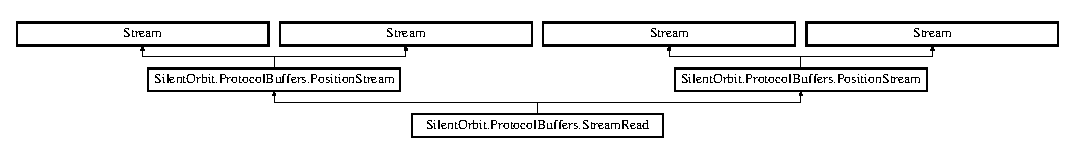
\includegraphics[height=1.627907cm]{class_silent_orbit_1_1_protocol_buffers_1_1_stream_read}
\end{center}
\end{figure}
\subsection*{Public Member Functions}
\begin{DoxyCompactItemize}
\item 
\hypertarget{class_silent_orbit_1_1_protocol_buffers_1_1_stream_read_a79f15b6f4801903fe6f4043e89d1b932}{}{\bfseries Stream\+Read} (Stream base\+Stream)\label{class_silent_orbit_1_1_protocol_buffers_1_1_stream_read_a79f15b6f4801903fe6f4043e89d1b932}

\item 
\hypertarget{class_silent_orbit_1_1_protocol_buffers_1_1_stream_read_a79f15b6f4801903fe6f4043e89d1b932}{}{\bfseries Stream\+Read} (Stream base\+Stream)\label{class_silent_orbit_1_1_protocol_buffers_1_1_stream_read_a79f15b6f4801903fe6f4043e89d1b932}

\end{DoxyCompactItemize}
\subsection*{Additional Inherited Members}


The documentation for this class was generated from the following file\+:\begin{DoxyCompactItemize}
\item 
/home/fpoole/development/cpe406/saas/cdti/\+C\+D\+T\+I\+Unity/\+Assets/scripts/Protocol\+Parser.\+cs\end{DoxyCompactItemize}

\hypertarget{class_json_1_1_stream_writer}{}\section{Json\+:\+:Stream\+Writer Class Reference}
\label{class_json_1_1_stream_writer}\index{Json\+::\+Stream\+Writer@{Json\+::\+Stream\+Writer}}


{\ttfamily \#include $<$json.\+h$>$}

Inheritance diagram for Json\+:\+:Stream\+Writer\+:\begin{figure}[H]
\begin{center}
\leavevmode
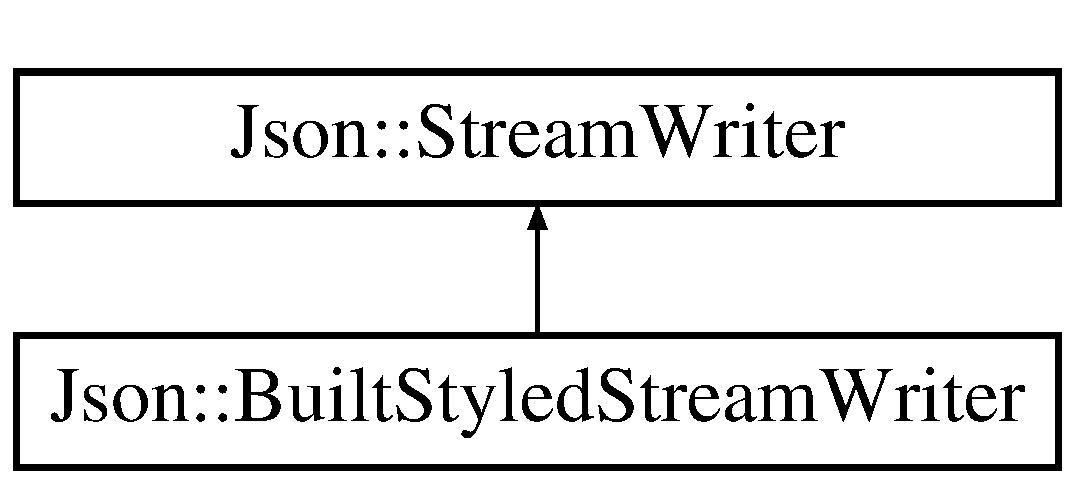
\includegraphics[height=2.000000cm]{class_json_1_1_stream_writer}
\end{center}
\end{figure}
\subsection*{Classes}
\begin{DoxyCompactItemize}
\item 
class \hyperlink{class_json_1_1_stream_writer_1_1_factory}{Factory}
\begin{DoxyCompactList}\small\item\em A simple abstract factory. \end{DoxyCompactList}\end{DoxyCompactItemize}
\subsection*{Public Member Functions}
\begin{DoxyCompactItemize}
\item 
virtual int \hyperlink{class_json_1_1_stream_writer_a237368cf13b41decc015640d25f176ab}{write} (\hyperlink{class_json_1_1_value}{Value} const \&root, std\+::ostream $\ast$sout)=0
\end{DoxyCompactItemize}
\subsection*{Protected Attributes}
\begin{DoxyCompactItemize}
\item 
\hypertarget{class_json_1_1_stream_writer_ac087569ccd2b5a22348cae92ec2a8996}{}std\+::ostream $\ast$ {\bfseries sout\+\_\+}\label{class_json_1_1_stream_writer_ac087569ccd2b5a22348cae92ec2a8996}

\end{DoxyCompactItemize}


\subsection{Detailed Description}
Usage\+: 
\begin{DoxyCode}
\textcolor{keyword}{using namespace }\hyperlink{namespace_json}{Json};
\textcolor{keywordtype}{void} writeToStdout(\hyperlink{class_json_1_1_stream_writer_1_1_factory}{StreamWriter::Factory} \textcolor{keyword}{const}& factory, 
      \hyperlink{class_json_1_1_value}{Value} \textcolor{keyword}{const}& value) \{
  std::unique\_ptr<StreamWriter> \textcolor{keyword}{const} writer(
    factory.\hyperlink{class_json_1_1_stream_writer_1_1_factory_a9d30ec53e8288cd53befccf1009c5f31}{newStreamWriter}());
  writer->write(value, &std::cout);
  std::cout << std::endl;  \textcolor{comment}{// add lf and flush}
\}
\end{DoxyCode}
 

\subsection{Member Function Documentation}
\hypertarget{class_json_1_1_stream_writer_a237368cf13b41decc015640d25f176ab}{}\index{Json\+::\+Stream\+Writer@{Json\+::\+Stream\+Writer}!write@{write}}
\index{write@{write}!Json\+::\+Stream\+Writer@{Json\+::\+Stream\+Writer}}
\subsubsection[{write}]{\setlength{\rightskip}{0pt plus 5cm}virtual int Json\+::\+Stream\+Writer\+::write (
\begin{DoxyParamCaption}
\item[{{\bf Value} const \&}]{root, }
\item[{std\+::ostream $\ast$}]{sout}
\end{DoxyParamCaption}
)\hspace{0.3cm}{\ttfamily [pure virtual]}}\label{class_json_1_1_stream_writer_a237368cf13b41decc015640d25f176ab}
Write \hyperlink{class_json_1_1_value}{Value} into document as configured in sub-\/class. Do not take ownership of sout, but maintain a reference during function. \begin{DoxyPrecond}{Precondition}
sout != N\+U\+L\+L 
\end{DoxyPrecond}
\begin{DoxyReturn}{Returns}
zero on success (For now, we always return zero, so check the stream instead.) 
\end{DoxyReturn}

\begin{DoxyExceptions}{Exceptions}
{\em std\+::exception} & possibly, depending on configuration \\
\hline
\end{DoxyExceptions}


Implemented in \hyperlink{struct_json_1_1_built_styled_stream_writer_a2ecffc3d66c4feddf208e5cd3b1c0f18}{Json\+::\+Built\+Styled\+Stream\+Writer}.



The documentation for this class was generated from the following files\+:\begin{DoxyCompactItemize}
\item 
/home/frank/dev/cpe402/saas/lib/jsoncpp/inc/json.\+h\item 
/home/frank/dev/cpe402/saas/lib/jsoncpp/src/jsoncpp.\+cpp\end{DoxyCompactItemize}

\hypertarget{class_json_1_1_stream_writer_builder}{}\section{Json\+:\+:Stream\+Writer\+Builder Class Reference}
\label{class_json_1_1_stream_writer_builder}\index{Json\+::\+Stream\+Writer\+Builder@{Json\+::\+Stream\+Writer\+Builder}}


Build a \hyperlink{class_json_1_1_stream_writer}{Stream\+Writer} implementation.  




{\ttfamily \#include $<$json.\+h$>$}

Inheritance diagram for Json\+:\+:Stream\+Writer\+Builder\+:\begin{figure}[H]
\begin{center}
\leavevmode
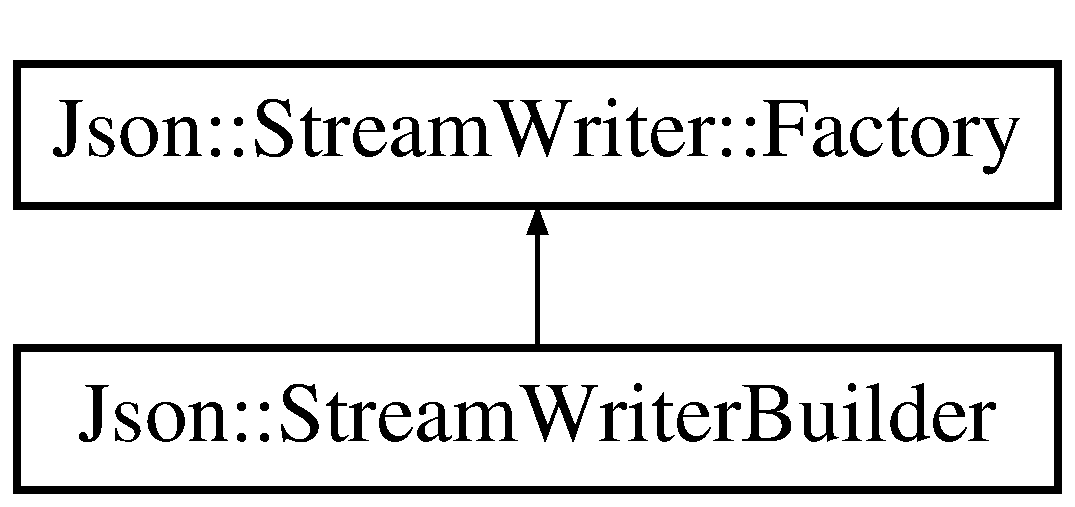
\includegraphics[height=2.000000cm]{class_json_1_1_stream_writer_builder}
\end{center}
\end{figure}
\subsection*{Public Member Functions}
\begin{DoxyCompactItemize}
\item 
\hyperlink{class_json_1_1_stream_writer}{Stream\+Writer} $\ast$ \hyperlink{class_json_1_1_stream_writer_builder_a042d21b84d8c5bede52a764e2ada7d65}{new\+Stream\+Writer} () const override
\item 
bool \hyperlink{class_json_1_1_stream_writer_builder_aa1dfed085a3d369e953e4a3c34da009e}{validate} (\hyperlink{class_json_1_1_value}{Json\+::\+Value} $\ast$invalid) const 
\item 
\hyperlink{class_json_1_1_value}{Value} \& \hyperlink{class_json_1_1_stream_writer_builder_aa010a8a04a92343179f64a5dbb5df340}{operator\mbox{[}$\,$\mbox{]}} (std\+::string key)
\end{DoxyCompactItemize}
\subsection*{Static Public Member Functions}
\begin{DoxyCompactItemize}
\item 
static void \hyperlink{class_json_1_1_stream_writer_builder_a53bf106b141e28637b01ad0ecd2acbf6}{set\+Defaults} (\hyperlink{class_json_1_1_value}{Json\+::\+Value} $\ast$settings)
\end{DoxyCompactItemize}
\subsection*{Public Attributes}
\begin{DoxyCompactItemize}
\item 
\hyperlink{class_json_1_1_value}{Json\+::\+Value} \hyperlink{class_json_1_1_stream_writer_builder_a79bdf2e639a52f4e758c0b95bd1d3423}{settings\+\_\+}
\end{DoxyCompactItemize}


\subsection{Detailed Description}
Build a \hyperlink{class_json_1_1_stream_writer}{Stream\+Writer} implementation. 

Usage\+: 
\begin{DoxyCode}
\textcolor{keyword}{using namespace }\hyperlink{namespace_json}{Json};
\hyperlink{class_json_1_1_value}{Value} value = ...;
\hyperlink{class_json_1_1_stream_writer_builder}{StreamWriterBuilder} builder;
builder[\textcolor{stringliteral}{"commentStyle"}] = \textcolor{stringliteral}{"None"};
builder[\textcolor{stringliteral}{"indentation"}] = \textcolor{stringliteral}{"   "};  \textcolor{comment}{// or whatever you like}
std::unique\_ptr<Json::StreamWriter> writer(
    builder.\hyperlink{class_json_1_1_stream_writer_builder_a042d21b84d8c5bede52a764e2ada7d65}{newStreamWriter}());
writer->write(value, &std::cout);
std::cout << std::endl;  \textcolor{comment}{// add lf and flush}
\end{DoxyCode}
 

\subsection{Member Function Documentation}
\hypertarget{class_json_1_1_stream_writer_builder_a042d21b84d8c5bede52a764e2ada7d65}{}\index{Json\+::\+Stream\+Writer\+Builder@{Json\+::\+Stream\+Writer\+Builder}!new\+Stream\+Writer@{new\+Stream\+Writer}}
\index{new\+Stream\+Writer@{new\+Stream\+Writer}!Json\+::\+Stream\+Writer\+Builder@{Json\+::\+Stream\+Writer\+Builder}}
\subsubsection[{new\+Stream\+Writer}]{\setlength{\rightskip}{0pt plus 5cm}{\bf Stream\+Writer} $\ast$ Json\+::\+Stream\+Writer\+Builder\+::new\+Stream\+Writer (
\begin{DoxyParamCaption}
{}
\end{DoxyParamCaption}
) const\hspace{0.3cm}{\ttfamily [override]}, {\ttfamily [virtual]}}\label{class_json_1_1_stream_writer_builder_a042d21b84d8c5bede52a764e2ada7d65}

\begin{DoxyExceptions}{Exceptions}
{\em std\+::exception} & if something goes wrong (e.\+g. invalid settings) \\
\hline
\end{DoxyExceptions}


Implements \hyperlink{class_json_1_1_stream_writer_1_1_factory_a9d30ec53e8288cd53befccf1009c5f31}{Json\+::\+Stream\+Writer\+::\+Factory}.

\hypertarget{class_json_1_1_stream_writer_builder_aa010a8a04a92343179f64a5dbb5df340}{}\index{Json\+::\+Stream\+Writer\+Builder@{Json\+::\+Stream\+Writer\+Builder}!operator\mbox{[}$\,$\mbox{]}@{operator[]}}
\index{operator\mbox{[}$\,$\mbox{]}@{operator[]}!Json\+::\+Stream\+Writer\+Builder@{Json\+::\+Stream\+Writer\+Builder}}
\subsubsection[{operator[]}]{\setlength{\rightskip}{0pt plus 5cm}{\bf Value} \& Json\+::\+Stream\+Writer\+Builder\+::operator\mbox{[}$\,$\mbox{]} (
\begin{DoxyParamCaption}
\item[{std\+::string}]{key}
\end{DoxyParamCaption}
)}\label{class_json_1_1_stream_writer_builder_aa010a8a04a92343179f64a5dbb5df340}
A simple way to update a specific setting. \hypertarget{class_json_1_1_stream_writer_builder_a53bf106b141e28637b01ad0ecd2acbf6}{}\index{Json\+::\+Stream\+Writer\+Builder@{Json\+::\+Stream\+Writer\+Builder}!set\+Defaults@{set\+Defaults}}
\index{set\+Defaults@{set\+Defaults}!Json\+::\+Stream\+Writer\+Builder@{Json\+::\+Stream\+Writer\+Builder}}
\subsubsection[{set\+Defaults}]{\setlength{\rightskip}{0pt plus 5cm}void Json\+::\+Stream\+Writer\+Builder\+::set\+Defaults (
\begin{DoxyParamCaption}
\item[{{\bf Json\+::\+Value} $\ast$}]{settings}
\end{DoxyParamCaption}
)\hspace{0.3cm}{\ttfamily [static]}}\label{class_json_1_1_stream_writer_builder_a53bf106b141e28637b01ad0ecd2acbf6}
Called by ctor, but you can use this to reset settings\+\_\+. \begin{DoxyPrecond}{Precondition}
\textquotesingle{}settings\textquotesingle{} != N\+U\+L\+L (but Json\+::null is fine) 
\end{DoxyPrecond}
\begin{DoxyRemark}{Remarks}
Defaults\+: 
\begin{DoxyCodeInclude}
\end{DoxyCodeInclude}

\end{DoxyRemark}
\mbox{[}Stream\+Writer\+Builder\+Defaults\mbox{]}

\mbox{[}Stream\+Writer\+Builder\+Defaults\mbox{]} \hypertarget{class_json_1_1_stream_writer_builder_aa1dfed085a3d369e953e4a3c34da009e}{}\index{Json\+::\+Stream\+Writer\+Builder@{Json\+::\+Stream\+Writer\+Builder}!validate@{validate}}
\index{validate@{validate}!Json\+::\+Stream\+Writer\+Builder@{Json\+::\+Stream\+Writer\+Builder}}
\subsubsection[{validate}]{\setlength{\rightskip}{0pt plus 5cm}bool Json\+::\+Stream\+Writer\+Builder\+::validate (
\begin{DoxyParamCaption}
\item[{{\bf Json\+::\+Value} $\ast$}]{invalid}
\end{DoxyParamCaption}
) const}\label{class_json_1_1_stream_writer_builder_aa1dfed085a3d369e953e4a3c34da009e}
\begin{DoxyReturn}{Returns}
true if \textquotesingle{}settings\textquotesingle{} are legal and consistent; otherwise, indicate bad settings via \textquotesingle{}invalid\textquotesingle{}. 
\end{DoxyReturn}


\subsection{Member Data Documentation}
\hypertarget{class_json_1_1_stream_writer_builder_a79bdf2e639a52f4e758c0b95bd1d3423}{}\index{Json\+::\+Stream\+Writer\+Builder@{Json\+::\+Stream\+Writer\+Builder}!settings\+\_\+@{settings\+\_\+}}
\index{settings\+\_\+@{settings\+\_\+}!Json\+::\+Stream\+Writer\+Builder@{Json\+::\+Stream\+Writer\+Builder}}
\subsubsection[{settings\+\_\+}]{\setlength{\rightskip}{0pt plus 5cm}{\bf Json\+::\+Value} Json\+::\+Stream\+Writer\+Builder\+::settings\+\_\+}\label{class_json_1_1_stream_writer_builder_a79bdf2e639a52f4e758c0b95bd1d3423}
Configuration of this builder. Available settings (case-\/sensitive)\+:
\begin{DoxyItemize}
\item \char`\"{}comment\+Style\char`\"{}\+: \char`\"{}\+None\char`\"{} or \char`\"{}\+All\char`\"{}
\item \char`\"{}indentation\char`\"{}\+: \char`\"{}$<$anything$>$\char`\"{}
\item \char`\"{}enable\+Y\+A\+M\+L\+Compatibility\char`\"{}\+: false or true
\begin{DoxyItemize}
\item slightly change the whitespace around colons
\end{DoxyItemize}
\item \char`\"{}drop\+Null\+Placeholders\char`\"{}\+: false or true
\begin{DoxyItemize}
\item Drop the \char`\"{}null\char`\"{} string from the writer\textquotesingle{}s output for null\+Values. Strictly speaking, this is not valid J\+S\+O\+N. But when the output is being fed to a browser\textquotesingle{}s Javascript, it makes for smaller output and the browser can handle the output just fine.
\end{DoxyItemize}
\item \char`\"{}use\+Special\+Floats\char`\"{}\+: false or true
\begin{DoxyItemize}
\item If true, outputs non-\/finite floating point values in the following way\+: Na\+N values as \char`\"{}\+Na\+N\char`\"{}, positive infinity as \char`\"{}\+Infinity\char`\"{}, and negative infinity as \char`\"{}-\/\+Infinity\char`\"{}.
\end{DoxyItemize}
\end{DoxyItemize}

You can examine \textquotesingle{}settings\+\_\+` yourself to see the defaults. You can also write and read them just like any J\+S\+O\+N \hyperlink{class_json_1_1_value}{Value}. \begin{DoxySeeAlso}{See also}
\hyperlink{class_json_1_1_stream_writer_builder_a53bf106b141e28637b01ad0ecd2acbf6}{set\+Defaults()} 
\end{DoxySeeAlso}


The documentation for this class was generated from the following files\+:\begin{DoxyCompactItemize}
\item 
/home/frank/dev/cpe402/saas/lib/jsoncpp/inc/json.\+h\item 
/home/frank/dev/cpe402/saas/lib/jsoncpp/src/jsoncpp.\+cpp\end{DoxyCompactItemize}

\hypertarget{struct_json_1_1_reader_1_1_structured_error}{}\section{Json\+:\+:Reader\+:\+:Structured\+Error Struct Reference}
\label{struct_json_1_1_reader_1_1_structured_error}\index{Json\+::\+Reader\+::\+Structured\+Error@{Json\+::\+Reader\+::\+Structured\+Error}}


An error tagged with where in the J\+S\+O\+N text it was encountered.  




{\ttfamily \#include $<$json.\+h$>$}

\subsection*{Public Attributes}
\begin{DoxyCompactItemize}
\item 
\hypertarget{struct_json_1_1_reader_1_1_structured_error_a160dae4eb3464a2209b743c755baf65f}{}size\+\_\+t {\bfseries offset\+\_\+start}\label{struct_json_1_1_reader_1_1_structured_error_a160dae4eb3464a2209b743c755baf65f}

\item 
\hypertarget{struct_json_1_1_reader_1_1_structured_error_a80747dae744bcc80a9bc81c94fd42e13}{}size\+\_\+t {\bfseries offset\+\_\+limit}\label{struct_json_1_1_reader_1_1_structured_error_a80747dae744bcc80a9bc81c94fd42e13}

\item 
\hypertarget{struct_json_1_1_reader_1_1_structured_error_ab8755e5201b78c6ae077338f8819e6e6}{}std\+::string {\bfseries message}\label{struct_json_1_1_reader_1_1_structured_error_ab8755e5201b78c6ae077338f8819e6e6}

\end{DoxyCompactItemize}


\subsection{Detailed Description}
An error tagged with where in the J\+S\+O\+N text it was encountered. 

The offsets give the \mbox{[}start, limit) range of bytes within the text. Note that this is bytes, not codepoints. 

The documentation for this struct was generated from the following file\+:\begin{DoxyCompactItemize}
\item 
/home/frank/dev/cpe402/saas/lib/jsoncpp/inc/json.\+h\end{DoxyCompactItemize}

\hypertarget{struct_json_1_1_our_reader_1_1_structured_error}{}\section{Json\+:\+:Our\+Reader\+:\+:Structured\+Error Struct Reference}
\label{struct_json_1_1_our_reader_1_1_structured_error}\index{Json\+::\+Our\+Reader\+::\+Structured\+Error@{Json\+::\+Our\+Reader\+::\+Structured\+Error}}
\subsection*{Public Attributes}
\begin{DoxyCompactItemize}
\item 
\hypertarget{struct_json_1_1_our_reader_1_1_structured_error_a4eec161c2a6b4c89b6eb3d8d83834443}{}size\+\_\+t {\bfseries offset\+\_\+start}\label{struct_json_1_1_our_reader_1_1_structured_error_a4eec161c2a6b4c89b6eb3d8d83834443}

\item 
\hypertarget{struct_json_1_1_our_reader_1_1_structured_error_a6bab2650e5230fc15427b309de79fdbe}{}size\+\_\+t {\bfseries offset\+\_\+limit}\label{struct_json_1_1_our_reader_1_1_structured_error_a6bab2650e5230fc15427b309de79fdbe}

\item 
\hypertarget{struct_json_1_1_our_reader_1_1_structured_error_adc8a757b6452cc6ab14fb90b933b3414}{}std\+::string {\bfseries message}\label{struct_json_1_1_our_reader_1_1_structured_error_adc8a757b6452cc6ab14fb90b933b3414}

\end{DoxyCompactItemize}


The documentation for this struct was generated from the following file\+:\begin{DoxyCompactItemize}
\item 
/home/frank/dev/cpe402/saas/lib/jsoncpp/src/jsoncpp.\+cpp\end{DoxyCompactItemize}

\hypertarget{class_json_1_1_styled_stream_writer}{}\section{Json\+:\+:Styled\+Stream\+Writer Class Reference}
\label{class_json_1_1_styled_stream_writer}\index{Json\+::\+Styled\+Stream\+Writer@{Json\+::\+Styled\+Stream\+Writer}}


Writes a \hyperlink{class_json_1_1_value}{Value} in \href{http://www.json.org}{\tt J\+S\+ON} format in a human friendly way, to a stream rather than to a string.  




{\ttfamily \#include $<$json.\+h$>$}

\subsection*{Public Member Functions}
\begin{DoxyCompactItemize}
\item 
{\bfseries Styled\+Stream\+Writer} (std\+::string indentation=\char`\"{}\textbackslash{}t\char`\"{})\hypertarget{class_json_1_1_styled_stream_writer_ae87567a08de865b6dc84d7218a3001df}{}\label{class_json_1_1_styled_stream_writer_ae87567a08de865b6dc84d7218a3001df}

\item 
void \hyperlink{class_json_1_1_styled_stream_writer_a07807741c6c43ecd35885a87234d0805}{write} (std\+::ostream \&out, const \hyperlink{class_json_1_1_value}{Value} \&root)
\begin{DoxyCompactList}\small\item\em Serialize a \hyperlink{class_json_1_1_value}{Value} in \href{http://www.json.org}{\tt J\+S\+ON} format. \end{DoxyCompactList}\end{DoxyCompactItemize}


\subsection{Detailed Description}
Writes a \hyperlink{class_json_1_1_value}{Value} in \href{http://www.json.org}{\tt J\+S\+ON} format in a human friendly way, to a stream rather than to a string. 

The rules for line break and indent are as follow\+:
\begin{DoxyItemize}
\item Object value\+:
\begin{DoxyItemize}
\item if empty then print \{\} without indent and line break
\item if not empty the print \textquotesingle{}\{\textquotesingle{}, line break \& indent, print one value per line and then unindent and line break and print \textquotesingle{}\}\textquotesingle{}.
\end{DoxyItemize}
\item Array value\+:
\begin{DoxyItemize}
\item if empty then print \mbox{[}\mbox{]} without indent and line break
\item if the array contains no object value, empty array or some other value types, and all the values fit on one lines, then print the array on a single line.
\item otherwise, it the values do not fit on one line, or the array contains object or non empty array, then print one value per line.
\end{DoxyItemize}
\end{DoxyItemize}

If the \hyperlink{class_json_1_1_value}{Value} have comments then they are outputed according to their \hyperlink{namespace_json_a4fc417c23905b2ae9e2c47d197a45351}{Comment\+Placement}.


\begin{DoxyParams}{Parameters}
{\em indentation} & Each level will be indented by this amount extra. \\
\hline
\end{DoxyParams}
\begin{DoxySeeAlso}{See also}
\hyperlink{class_json_1_1_reader}{Reader}, \hyperlink{class_json_1_1_value}{Value}, \hyperlink{class_json_1_1_value_a29f3a30f7e5d3af6f38d57999bf5b480}{Value\+::set\+Comment()} 
\end{DoxySeeAlso}
\begin{DoxyRefDesc}{Deprecated}
\item[\hyperlink{deprecated__deprecated000010}{Deprecated}]Use \hyperlink{class_json_1_1_stream_writer_builder}{Stream\+Writer\+Builder}. \end{DoxyRefDesc}


\subsection{Member Function Documentation}
\index{Json\+::\+Styled\+Stream\+Writer@{Json\+::\+Styled\+Stream\+Writer}!write@{write}}
\index{write@{write}!Json\+::\+Styled\+Stream\+Writer@{Json\+::\+Styled\+Stream\+Writer}}
\subsubsection[{\texorpdfstring{write(std\+::ostream \&out, const Value \&root)}{write(std::ostream &out, const Value &root)}}]{\setlength{\rightskip}{0pt plus 5cm}void Json\+::\+Styled\+Stream\+Writer\+::write (
\begin{DoxyParamCaption}
\item[{std\+::ostream \&}]{out, }
\item[{const {\bf Value} \&}]{root}
\end{DoxyParamCaption}
)}\hypertarget{class_json_1_1_styled_stream_writer_a07807741c6c43ecd35885a87234d0805}{}\label{class_json_1_1_styled_stream_writer_a07807741c6c43ecd35885a87234d0805}


Serialize a \hyperlink{class_json_1_1_value}{Value} in \href{http://www.json.org}{\tt J\+S\+ON} format. 


\begin{DoxyParams}{Parameters}
{\em out} & Stream to write to. (Can be ostringstream, e.\+g.) \\
\hline
{\em root} & \hyperlink{class_json_1_1_value}{Value} to serialize. \\
\hline
\end{DoxyParams}
\begin{DoxyNote}{Note}
There is no point in deriving from \hyperlink{class_json_1_1_writer}{Writer}, since \hyperlink{class_json_1_1_styled_stream_writer_a07807741c6c43ecd35885a87234d0805}{write()} should not return a value. 
\end{DoxyNote}


The documentation for this class was generated from the following files\+:\begin{DoxyCompactItemize}
\item 
/home/andrea/\+Clion\+Projects/saas/lib/jsoncpp/inc/json.\+h\item 
/home/andrea/\+Clion\+Projects/saas/lib/jsoncpp/src/jsoncpp.\+cpp\end{DoxyCompactItemize}

\hypertarget{class_json_1_1_styled_writer}{}\section{Json\+:\+:Styled\+Writer Class Reference}
\label{class_json_1_1_styled_writer}\index{Json\+::\+Styled\+Writer@{Json\+::\+Styled\+Writer}}


Writes a \hyperlink{class_json_1_1_value}{Value} in \href{http://www.json.org}{\tt J\+S\+O\+N} format in a human friendly way.  




{\ttfamily \#include $<$json.\+h$>$}

Inheritance diagram for Json\+:\+:Styled\+Writer\+:\begin{figure}[H]
\begin{center}
\leavevmode
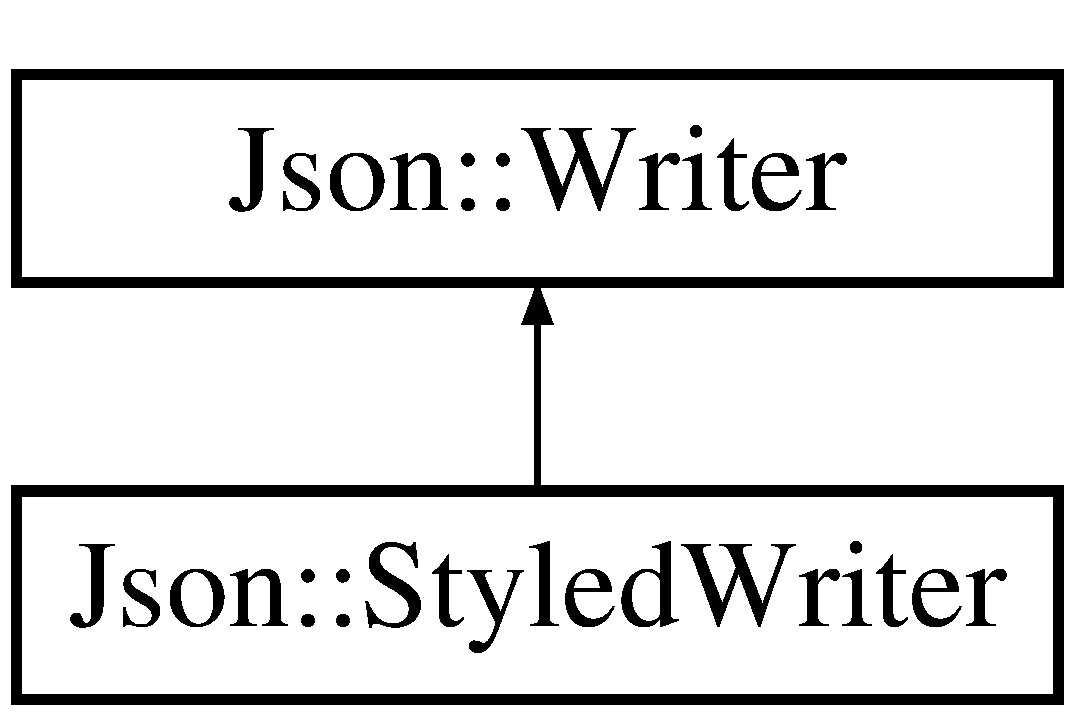
\includegraphics[height=2.000000cm]{class_json_1_1_styled_writer}
\end{center}
\end{figure}
\subsection*{Public Member Functions}
\begin{DoxyCompactItemize}
\item 
std\+::string \hyperlink{class_json_1_1_styled_writer_abd42ae0b8a788a46969fc51a28a496f5}{write} (const \hyperlink{class_json_1_1_value}{Value} \&root) override
\begin{DoxyCompactList}\small\item\em Serialize a \hyperlink{class_json_1_1_value}{Value} in \href{http://www.json.org}{\tt J\+S\+O\+N} format. \end{DoxyCompactList}\end{DoxyCompactItemize}


\subsection{Detailed Description}
Writes a \hyperlink{class_json_1_1_value}{Value} in \href{http://www.json.org}{\tt J\+S\+O\+N} format in a human friendly way. 

The rules for line break and indent are as follow\+:
\begin{DoxyItemize}
\item Object value\+:
\begin{DoxyItemize}
\item if empty then print \{\} without indent and line break
\item if not empty the print \textquotesingle{}\{\textquotesingle{}, line break \& indent, print one value per line and then unindent and line break and print \textquotesingle{}\}\textquotesingle{}.
\end{DoxyItemize}
\item Array value\+:
\begin{DoxyItemize}
\item if empty then print \mbox{[}\mbox{]} without indent and line break
\item if the array contains no object value, empty array or some other value types, and all the values fit on one lines, then print the array on a single line.
\item otherwise, it the values do not fit on one line, or the array contains object or non empty array, then print one value per line.
\end{DoxyItemize}
\end{DoxyItemize}

If the \hyperlink{class_json_1_1_value}{Value} have comments then they are outputed according to their \hyperlink{namespace_json_a4fc417c23905b2ae9e2c47d197a45351}{Comment\+Placement}.

\begin{DoxySeeAlso}{See also}
\hyperlink{class_json_1_1_reader}{Reader}, \hyperlink{class_json_1_1_value}{Value}, \hyperlink{class_json_1_1_value_a29f3a30f7e5d3af6f38d57999bf5b480}{Value\+::set\+Comment()} 
\end{DoxySeeAlso}
\begin{DoxyRefDesc}{Deprecated}
\item[\hyperlink{deprecated__deprecated000009}{Deprecated}]Use \hyperlink{class_json_1_1_stream_writer_builder}{Stream\+Writer\+Builder}. \end{DoxyRefDesc}


\subsection{Member Function Documentation}
\hypertarget{class_json_1_1_styled_writer_abd42ae0b8a788a46969fc51a28a496f5}{}\index{Json\+::\+Styled\+Writer@{Json\+::\+Styled\+Writer}!write@{write}}
\index{write@{write}!Json\+::\+Styled\+Writer@{Json\+::\+Styled\+Writer}}
\subsubsection[{write}]{\setlength{\rightskip}{0pt plus 5cm}std\+::string Json\+::\+Styled\+Writer\+::write (
\begin{DoxyParamCaption}
\item[{const {\bf Value} \&}]{root}
\end{DoxyParamCaption}
)\hspace{0.3cm}{\ttfamily [override]}, {\ttfamily [virtual]}}\label{class_json_1_1_styled_writer_abd42ae0b8a788a46969fc51a28a496f5}


Serialize a \hyperlink{class_json_1_1_value}{Value} in \href{http://www.json.org}{\tt J\+S\+O\+N} format. 


\begin{DoxyParams}{Parameters}
{\em root} & \hyperlink{class_json_1_1_value}{Value} to serialize. \\
\hline
\end{DoxyParams}
\begin{DoxyReturn}{Returns}
String containing the J\+S\+O\+N document that represents the root value. 
\end{DoxyReturn}


Implements \hyperlink{class_json_1_1_writer}{Json\+::\+Writer}.



The documentation for this class was generated from the following files\+:\begin{DoxyCompactItemize}
\item 
/home/fpoole/development/cpe406/saas/lib/jsoncpp/inc/json.\+h\item 
/home/fpoole/development/cpe406/saas/lib/jsoncpp/src/jsoncpp.\+cpp\end{DoxyCompactItemize}

\input{struct_surveillance_report}
\hypertarget{class_ciela_spike_1_1_task}{}\section{Ciela\+Spike.\+Task Class Reference}
\label{class_ciela_spike_1_1_task}\index{Ciela\+Spike.\+Task@{Ciela\+Spike.\+Task}}


Represents an async task.  


Inheritance diagram for Ciela\+Spike.\+Task\+:\begin{figure}[H]
\begin{center}
\leavevmode
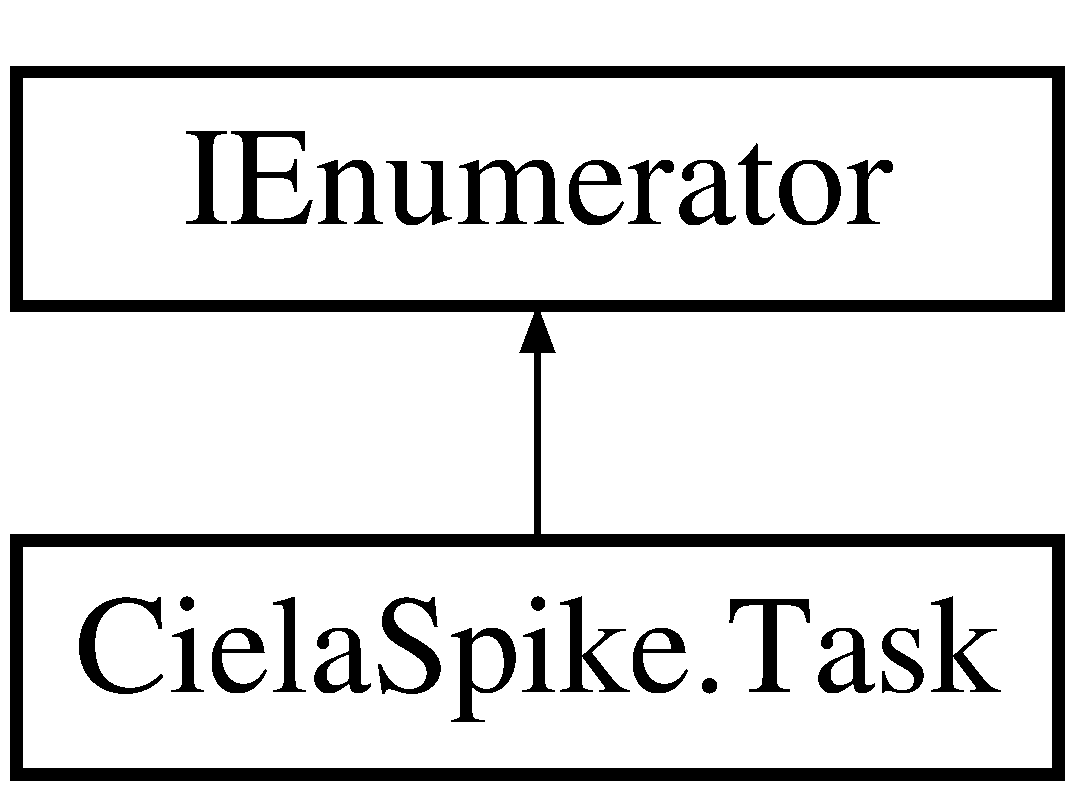
\includegraphics[height=2.000000cm]{class_ciela_spike_1_1_task}
\end{center}
\end{figure}
\subsection*{Public Member Functions}
\begin{DoxyCompactItemize}
\item 
bool \hyperlink{class_ciela_spike_1_1_task_a7aa5e9ac9431e14540db93eadbbedd3f}{Move\+Next} ()
\begin{DoxyCompactList}\small\item\em Runs next iteration. \end{DoxyCompactList}\item 
void {\bfseries Reset} ()\hypertarget{class_ciela_spike_1_1_task_abaa2e386621a8490e72f325d7a29920b}{}\label{class_ciela_spike_1_1_task_abaa2e386621a8490e72f325d7a29920b}

\item 
{\bfseries Task} (I\+Enumerator routine)\hypertarget{class_ciela_spike_1_1_task_a93dd2db76a6f8476fa1bdf4698827df6}{}\label{class_ciela_spike_1_1_task_a93dd2db76a6f8476fa1bdf4698827df6}

\item 
void \hyperlink{class_ciela_spike_1_1_task_a441c75316841dbb5efef5902410d77d9}{Cancel} ()
\begin{DoxyCompactList}\small\item\em Cancel the task till next iteration; \end{DoxyCompactList}\item 
I\+Enumerator \hyperlink{class_ciela_spike_1_1_task_aabec45633d71b685190331089f612392}{Wait} ()
\begin{DoxyCompactList}\small\item\em A co-\/routine that waits the task. \end{DoxyCompactList}\end{DoxyCompactItemize}
\subsection*{Properties}
\begin{DoxyCompactItemize}
\item 
object \hyperlink{class_ciela_spike_1_1_task_a1b998f7aa927571627df0e146693c5a4}{Current}\hspace{0.3cm}{\ttfamily  \mbox{[}get\mbox{]}}
\begin{DoxyCompactList}\small\item\em The current iterator yield return value. \end{DoxyCompactList}\item 
\hyperlink{namespace_ciela_spike_a4782eb2c0b65a1d593a94740bf994960}{Task\+State} \hyperlink{class_ciela_spike_1_1_task_a0b9fb190966ab28515afb40541ba23cf}{State}\hspace{0.3cm}{\ttfamily  \mbox{[}get\mbox{]}}
\begin{DoxyCompactList}\small\item\em Gets state of the task. \end{DoxyCompactList}\item 
System.\+Exception \hyperlink{class_ciela_spike_1_1_task_a16f755d6c2d90b3d528aebc7526a0a2b}{Exception}\hspace{0.3cm}{\ttfamily  \mbox{[}get\mbox{]}}
\begin{DoxyCompactList}\small\item\em Gets exception during running. \end{DoxyCompactList}\end{DoxyCompactItemize}


\subsection{Detailed Description}
Represents an async task. 



\subsection{Member Function Documentation}
\index{Ciela\+Spike\+::\+Task@{Ciela\+Spike\+::\+Task}!Cancel@{Cancel}}
\index{Cancel@{Cancel}!Ciela\+Spike\+::\+Task@{Ciela\+Spike\+::\+Task}}
\subsubsection[{\texorpdfstring{Cancel()}{Cancel()}}]{\setlength{\rightskip}{0pt plus 5cm}void Ciela\+Spike.\+Task.\+Cancel (
\begin{DoxyParamCaption}
{}
\end{DoxyParamCaption}
)\hspace{0.3cm}{\ttfamily [inline]}}\hypertarget{class_ciela_spike_1_1_task_a441c75316841dbb5efef5902410d77d9}{}\label{class_ciela_spike_1_1_task_a441c75316841dbb5efef5902410d77d9}


Cancel the task till next iteration; 

\index{Ciela\+Spike\+::\+Task@{Ciela\+Spike\+::\+Task}!Move\+Next@{Move\+Next}}
\index{Move\+Next@{Move\+Next}!Ciela\+Spike\+::\+Task@{Ciela\+Spike\+::\+Task}}
\subsubsection[{\texorpdfstring{Move\+Next()}{MoveNext()}}]{\setlength{\rightskip}{0pt plus 5cm}bool Ciela\+Spike.\+Task.\+Move\+Next (
\begin{DoxyParamCaption}
{}
\end{DoxyParamCaption}
)\hspace{0.3cm}{\ttfamily [inline]}}\hypertarget{class_ciela_spike_1_1_task_a7aa5e9ac9431e14540db93eadbbedd3f}{}\label{class_ciela_spike_1_1_task_a7aa5e9ac9431e14540db93eadbbedd3f}


Runs next iteration. 

\begin{DoxyReturn}{Returns}

\begin{DoxyCode}
\textcolor{keyword}{true}
\end{DoxyCode}
 for continue, otherwise 
\begin{DoxyCode}
\textcolor{keyword}{false}
\end{DoxyCode}
.
\end{DoxyReturn}
\index{Ciela\+Spike\+::\+Task@{Ciela\+Spike\+::\+Task}!Wait@{Wait}}
\index{Wait@{Wait}!Ciela\+Spike\+::\+Task@{Ciela\+Spike\+::\+Task}}
\subsubsection[{\texorpdfstring{Wait()}{Wait()}}]{\setlength{\rightskip}{0pt plus 5cm}I\+Enumerator Ciela\+Spike.\+Task.\+Wait (
\begin{DoxyParamCaption}
{}
\end{DoxyParamCaption}
)\hspace{0.3cm}{\ttfamily [inline]}}\hypertarget{class_ciela_spike_1_1_task_aabec45633d71b685190331089f612392}{}\label{class_ciela_spike_1_1_task_aabec45633d71b685190331089f612392}


A co-\/routine that waits the task. 



\subsection{Property Documentation}
\index{Ciela\+Spike\+::\+Task@{Ciela\+Spike\+::\+Task}!Current@{Current}}
\index{Current@{Current}!Ciela\+Spike\+::\+Task@{Ciela\+Spike\+::\+Task}}
\subsubsection[{\texorpdfstring{Current}{Current}}]{\setlength{\rightskip}{0pt plus 5cm}object Ciela\+Spike.\+Task.\+Current\hspace{0.3cm}{\ttfamily [get]}}\hypertarget{class_ciela_spike_1_1_task_a1b998f7aa927571627df0e146693c5a4}{}\label{class_ciela_spike_1_1_task_a1b998f7aa927571627df0e146693c5a4}


The current iterator yield return value. 

\index{Ciela\+Spike\+::\+Task@{Ciela\+Spike\+::\+Task}!Exception@{Exception}}
\index{Exception@{Exception}!Ciela\+Spike\+::\+Task@{Ciela\+Spike\+::\+Task}}
\subsubsection[{\texorpdfstring{Exception}{Exception}}]{\setlength{\rightskip}{0pt plus 5cm}System.\+Exception Ciela\+Spike.\+Task.\+Exception\hspace{0.3cm}{\ttfamily [get]}}\hypertarget{class_ciela_spike_1_1_task_a16f755d6c2d90b3d528aebc7526a0a2b}{}\label{class_ciela_spike_1_1_task_a16f755d6c2d90b3d528aebc7526a0a2b}


Gets exception during running. 

\index{Ciela\+Spike\+::\+Task@{Ciela\+Spike\+::\+Task}!State@{State}}
\index{State@{State}!Ciela\+Spike\+::\+Task@{Ciela\+Spike\+::\+Task}}
\subsubsection[{\texorpdfstring{State}{State}}]{\setlength{\rightskip}{0pt plus 5cm}{\bf Task\+State} Ciela\+Spike.\+Task.\+State\hspace{0.3cm}{\ttfamily [get]}}\hypertarget{class_ciela_spike_1_1_task_a0b9fb190966ab28515afb40541ba23cf}{}\label{class_ciela_spike_1_1_task_a0b9fb190966ab28515afb40541ba23cf}


Gets state of the task. 



The documentation for this class was generated from the following file\+:\begin{DoxyCompactItemize}
\item 
/\+Users/\+Dat/\+Clion\+Projects/saas/cdti/\+C\+D\+T\+I\+Unity/\+Assets/\+Ciela\+Spike/\+Thread Ninja/Task.\+cs\end{DoxyCompactItemize}

\hypertarget{class_example_1_1_tcas_report}{}\section{Example.\+Tcas\+Report Class Reference}
\label{class_example_1_1_tcas_report}\index{Example.\+Tcas\+Report@{Example.\+Tcas\+Report}}
\subsection*{Static Public Member Functions}
\begin{DoxyCompactItemize}
\item 
static \hyperlink{class_example_1_1_tcas_report}{Tcas\+Report} \hyperlink{class_example_1_1_tcas_report_a226662cf1becc0b4e5c94bb677fe3cb7}{Deserialize} (Stream stream)
\begin{DoxyCompactList}\small\item\em Helper\+: create a new instance to deserializing into\end{DoxyCompactList}\item 
static \hyperlink{class_example_1_1_tcas_report}{Tcas\+Report} \hyperlink{class_example_1_1_tcas_report_a11671313adb628266647791e54f33566}{Deserialize\+Length\+Delimited} (Stream stream)
\begin{DoxyCompactList}\small\item\em Helper\+: create a new instance to deserializing into\end{DoxyCompactList}\item 
static \hyperlink{class_example_1_1_tcas_report}{Tcas\+Report} \hyperlink{class_example_1_1_tcas_report_aafbcd33afecb9bc0511bdb14f0121dd0}{Deserialize\+Length} (Stream stream, int length)
\begin{DoxyCompactList}\small\item\em Helper\+: create a new instance to deserializing into\end{DoxyCompactList}\item 
static \hyperlink{class_example_1_1_tcas_report}{Tcas\+Report} \hyperlink{class_example_1_1_tcas_report_a95a21b26286e534445e670310b216a15}{Deserialize} (byte\mbox{[}$\,$\mbox{]} buffer)
\begin{DoxyCompactList}\small\item\em Helper\+: put the buffer into a Memory\+Stream and create a new instance to deserializing into\end{DoxyCompactList}\item 
static \hyperlink{class_example_1_1_tcas_report}{Example.\+Tcas\+Report} \hyperlink{class_example_1_1_tcas_report_a75d7b4ddbb76dd34dd8f5389a4b78f5a}{Deserialize} (byte\mbox{[}$\,$\mbox{]} buffer, \hyperlink{class_example_1_1_tcas_report}{Example.\+Tcas\+Report} instance)
\begin{DoxyCompactList}\small\item\em Helper\+: put the buffer into a Memory\+Stream before deserializing\end{DoxyCompactList}\item 
static \hyperlink{class_example_1_1_tcas_report}{Example.\+Tcas\+Report} \hyperlink{class_example_1_1_tcas_report_ab155a0521aabdf8a0ef91cd1a4932aa1}{Deserialize} (Stream stream, \hyperlink{class_example_1_1_tcas_report}{Example.\+Tcas\+Report} instance)
\begin{DoxyCompactList}\small\item\em Takes the remaining content of the stream and deserialze it into the instance.\end{DoxyCompactList}\item 
static \hyperlink{class_example_1_1_tcas_report}{Example.\+Tcas\+Report} \hyperlink{class_example_1_1_tcas_report_a19357c6915072658c1bdb5e4969acee6}{Deserialize\+Length\+Delimited} (Stream stream, \hyperlink{class_example_1_1_tcas_report}{Example.\+Tcas\+Report} instance)
\begin{DoxyCompactList}\small\item\em Read the Var\+Int length prefix and the given number of bytes from the stream and deserialze it into the instance.\end{DoxyCompactList}\item 
static \hyperlink{class_example_1_1_tcas_report}{Example.\+Tcas\+Report} \hyperlink{class_example_1_1_tcas_report_a9c164eb47708f5c254c6b793de0efd91}{Deserialize\+Length} (Stream stream, int length, \hyperlink{class_example_1_1_tcas_report}{Example.\+Tcas\+Report} instance)
\begin{DoxyCompactList}\small\item\em Read the given number of bytes from the stream and deserialze it into the instance.\end{DoxyCompactList}\item 
static void \hyperlink{class_example_1_1_tcas_report_a54cf22e91a20b051dc9b50be3292f0c2}{Serialize} (Stream stream, \hyperlink{class_example_1_1_tcas_report}{Tcas\+Report} instance)
\begin{DoxyCompactList}\small\item\em Serialize the instance into the stream\end{DoxyCompactList}\item 
static byte\mbox{[}$\,$\mbox{]} \hyperlink{class_example_1_1_tcas_report_aad7a3320484bf00a2f238c95d61cb2f5}{Serialize\+To\+Bytes} (\hyperlink{class_example_1_1_tcas_report}{Tcas\+Report} instance)
\begin{DoxyCompactList}\small\item\em Helper\+: Serialize into a Memory\+Stream and return its byte array\end{DoxyCompactList}\item 
static void \hyperlink{class_example_1_1_tcas_report_a65c3a0268ceb68df8be04522cbadd029}{Serialize\+Length\+Delimited} (Stream stream, \hyperlink{class_example_1_1_tcas_report}{Tcas\+Report} instance)
\begin{DoxyCompactList}\small\item\em Helper\+: Serialize with a varint length prefix\end{DoxyCompactList}\end{DoxyCompactItemize}
\subsection*{Properties}
\begin{DoxyCompactItemize}
\item 
int {\bfseries Id}\hspace{0.3cm}{\ttfamily  \mbox{[}get, set\mbox{]}}\hypertarget{class_example_1_1_tcas_report_abae87180b605bd602950494bb76e7f56}{}\label{class_example_1_1_tcas_report_abae87180b605bd602950494bb76e7f56}

\item 
int \hyperlink{class_example_1_1_tcas_report_a32691ce0bb3b627f44655cf3013f5f20}{Range}\hspace{0.3cm}{\ttfamily  \mbox{[}get, set\mbox{]}}
\begin{DoxyCompactList}\small\item\em ID of target\end{DoxyCompactList}\item 
int \hyperlink{class_example_1_1_tcas_report_a88be13f8636f9e7902c325ec73a150f8}{Altitude}\hspace{0.3cm}{\ttfamily  \mbox{[}get, set\mbox{]}}
\begin{DoxyCompactList}\small\item\em relative distance\end{DoxyCompactList}\item 
int \hyperlink{class_example_1_1_tcas_report_a12eb2351e84f8e2830223829fde681ad}{Bearing}\hspace{0.3cm}{\ttfamily  \mbox{[}get, set\mbox{]}}
\begin{DoxyCompactList}\small\item\em relative altitude\end{DoxyCompactList}\end{DoxyCompactItemize}


\subsection{Member Function Documentation}
\index{Example\+::\+Tcas\+Report@{Example\+::\+Tcas\+Report}!Deserialize@{Deserialize}}
\index{Deserialize@{Deserialize}!Example\+::\+Tcas\+Report@{Example\+::\+Tcas\+Report}}
\subsubsection[{\texorpdfstring{Deserialize(\+Stream stream)}{Deserialize(Stream stream)}}]{\setlength{\rightskip}{0pt plus 5cm}static {\bf Tcas\+Report} Example.\+Tcas\+Report.\+Deserialize (
\begin{DoxyParamCaption}
\item[{Stream}]{stream}
\end{DoxyParamCaption}
)\hspace{0.3cm}{\ttfamily [inline]}, {\ttfamily [static]}}\hypertarget{class_example_1_1_tcas_report_a226662cf1becc0b4e5c94bb677fe3cb7}{}\label{class_example_1_1_tcas_report_a226662cf1becc0b4e5c94bb677fe3cb7}


Helper\+: create a new instance to deserializing into

\index{Example\+::\+Tcas\+Report@{Example\+::\+Tcas\+Report}!Deserialize@{Deserialize}}
\index{Deserialize@{Deserialize}!Example\+::\+Tcas\+Report@{Example\+::\+Tcas\+Report}}
\subsubsection[{\texorpdfstring{Deserialize(byte[] buffer)}{Deserialize(byte[] buffer)}}]{\setlength{\rightskip}{0pt plus 5cm}static {\bf Tcas\+Report} Example.\+Tcas\+Report.\+Deserialize (
\begin{DoxyParamCaption}
\item[{byte\mbox{[}$\,$\mbox{]}}]{buffer}
\end{DoxyParamCaption}
)\hspace{0.3cm}{\ttfamily [inline]}, {\ttfamily [static]}}\hypertarget{class_example_1_1_tcas_report_a95a21b26286e534445e670310b216a15}{}\label{class_example_1_1_tcas_report_a95a21b26286e534445e670310b216a15}


Helper\+: put the buffer into a Memory\+Stream and create a new instance to deserializing into

\index{Example\+::\+Tcas\+Report@{Example\+::\+Tcas\+Report}!Deserialize@{Deserialize}}
\index{Deserialize@{Deserialize}!Example\+::\+Tcas\+Report@{Example\+::\+Tcas\+Report}}
\subsubsection[{\texorpdfstring{Deserialize(byte[] buffer, Example.\+Tcas\+Report instance)}{Deserialize(byte[] buffer, Example.TcasReport instance)}}]{\setlength{\rightskip}{0pt plus 5cm}static {\bf Example.\+Tcas\+Report} Example.\+Tcas\+Report.\+Deserialize (
\begin{DoxyParamCaption}
\item[{byte\mbox{[}$\,$\mbox{]}}]{buffer, }
\item[{{\bf Example.\+Tcas\+Report}}]{instance}
\end{DoxyParamCaption}
)\hspace{0.3cm}{\ttfamily [inline]}, {\ttfamily [static]}}\hypertarget{class_example_1_1_tcas_report_a75d7b4ddbb76dd34dd8f5389a4b78f5a}{}\label{class_example_1_1_tcas_report_a75d7b4ddbb76dd34dd8f5389a4b78f5a}


Helper\+: put the buffer into a Memory\+Stream before deserializing

\index{Example\+::\+Tcas\+Report@{Example\+::\+Tcas\+Report}!Deserialize@{Deserialize}}
\index{Deserialize@{Deserialize}!Example\+::\+Tcas\+Report@{Example\+::\+Tcas\+Report}}
\subsubsection[{\texorpdfstring{Deserialize(\+Stream stream, Example.\+Tcas\+Report instance)}{Deserialize(Stream stream, Example.TcasReport instance)}}]{\setlength{\rightskip}{0pt plus 5cm}static {\bf Example.\+Tcas\+Report} Example.\+Tcas\+Report.\+Deserialize (
\begin{DoxyParamCaption}
\item[{Stream}]{stream, }
\item[{{\bf Example.\+Tcas\+Report}}]{instance}
\end{DoxyParamCaption}
)\hspace{0.3cm}{\ttfamily [inline]}, {\ttfamily [static]}}\hypertarget{class_example_1_1_tcas_report_ab155a0521aabdf8a0ef91cd1a4932aa1}{}\label{class_example_1_1_tcas_report_ab155a0521aabdf8a0ef91cd1a4932aa1}


Takes the remaining content of the stream and deserialze it into the instance.

\index{Example\+::\+Tcas\+Report@{Example\+::\+Tcas\+Report}!Deserialize\+Length@{Deserialize\+Length}}
\index{Deserialize\+Length@{Deserialize\+Length}!Example\+::\+Tcas\+Report@{Example\+::\+Tcas\+Report}}
\subsubsection[{\texorpdfstring{Deserialize\+Length(\+Stream stream, int length)}{DeserializeLength(Stream stream, int length)}}]{\setlength{\rightskip}{0pt plus 5cm}static {\bf Tcas\+Report} Example.\+Tcas\+Report.\+Deserialize\+Length (
\begin{DoxyParamCaption}
\item[{Stream}]{stream, }
\item[{int}]{length}
\end{DoxyParamCaption}
)\hspace{0.3cm}{\ttfamily [inline]}, {\ttfamily [static]}}\hypertarget{class_example_1_1_tcas_report_aafbcd33afecb9bc0511bdb14f0121dd0}{}\label{class_example_1_1_tcas_report_aafbcd33afecb9bc0511bdb14f0121dd0}


Helper\+: create a new instance to deserializing into

\index{Example\+::\+Tcas\+Report@{Example\+::\+Tcas\+Report}!Deserialize\+Length@{Deserialize\+Length}}
\index{Deserialize\+Length@{Deserialize\+Length}!Example\+::\+Tcas\+Report@{Example\+::\+Tcas\+Report}}
\subsubsection[{\texorpdfstring{Deserialize\+Length(\+Stream stream, int length, Example.\+Tcas\+Report instance)}{DeserializeLength(Stream stream, int length, Example.TcasReport instance)}}]{\setlength{\rightskip}{0pt plus 5cm}static {\bf Example.\+Tcas\+Report} Example.\+Tcas\+Report.\+Deserialize\+Length (
\begin{DoxyParamCaption}
\item[{Stream}]{stream, }
\item[{int}]{length, }
\item[{{\bf Example.\+Tcas\+Report}}]{instance}
\end{DoxyParamCaption}
)\hspace{0.3cm}{\ttfamily [inline]}, {\ttfamily [static]}}\hypertarget{class_example_1_1_tcas_report_a9c164eb47708f5c254c6b793de0efd91}{}\label{class_example_1_1_tcas_report_a9c164eb47708f5c254c6b793de0efd91}


Read the given number of bytes from the stream and deserialze it into the instance.

\index{Example\+::\+Tcas\+Report@{Example\+::\+Tcas\+Report}!Deserialize\+Length\+Delimited@{Deserialize\+Length\+Delimited}}
\index{Deserialize\+Length\+Delimited@{Deserialize\+Length\+Delimited}!Example\+::\+Tcas\+Report@{Example\+::\+Tcas\+Report}}
\subsubsection[{\texorpdfstring{Deserialize\+Length\+Delimited(\+Stream stream)}{DeserializeLengthDelimited(Stream stream)}}]{\setlength{\rightskip}{0pt plus 5cm}static {\bf Tcas\+Report} Example.\+Tcas\+Report.\+Deserialize\+Length\+Delimited (
\begin{DoxyParamCaption}
\item[{Stream}]{stream}
\end{DoxyParamCaption}
)\hspace{0.3cm}{\ttfamily [inline]}, {\ttfamily [static]}}\hypertarget{class_example_1_1_tcas_report_a11671313adb628266647791e54f33566}{}\label{class_example_1_1_tcas_report_a11671313adb628266647791e54f33566}


Helper\+: create a new instance to deserializing into

\index{Example\+::\+Tcas\+Report@{Example\+::\+Tcas\+Report}!Deserialize\+Length\+Delimited@{Deserialize\+Length\+Delimited}}
\index{Deserialize\+Length\+Delimited@{Deserialize\+Length\+Delimited}!Example\+::\+Tcas\+Report@{Example\+::\+Tcas\+Report}}
\subsubsection[{\texorpdfstring{Deserialize\+Length\+Delimited(\+Stream stream, Example.\+Tcas\+Report instance)}{DeserializeLengthDelimited(Stream stream, Example.TcasReport instance)}}]{\setlength{\rightskip}{0pt plus 5cm}static {\bf Example.\+Tcas\+Report} Example.\+Tcas\+Report.\+Deserialize\+Length\+Delimited (
\begin{DoxyParamCaption}
\item[{Stream}]{stream, }
\item[{{\bf Example.\+Tcas\+Report}}]{instance}
\end{DoxyParamCaption}
)\hspace{0.3cm}{\ttfamily [inline]}, {\ttfamily [static]}}\hypertarget{class_example_1_1_tcas_report_a19357c6915072658c1bdb5e4969acee6}{}\label{class_example_1_1_tcas_report_a19357c6915072658c1bdb5e4969acee6}


Read the Var\+Int length prefix and the given number of bytes from the stream and deserialze it into the instance.

\index{Example\+::\+Tcas\+Report@{Example\+::\+Tcas\+Report}!Serialize@{Serialize}}
\index{Serialize@{Serialize}!Example\+::\+Tcas\+Report@{Example\+::\+Tcas\+Report}}
\subsubsection[{\texorpdfstring{Serialize(\+Stream stream, Tcas\+Report instance)}{Serialize(Stream stream, TcasReport instance)}}]{\setlength{\rightskip}{0pt plus 5cm}static void Example.\+Tcas\+Report.\+Serialize (
\begin{DoxyParamCaption}
\item[{Stream}]{stream, }
\item[{{\bf Tcas\+Report}}]{instance}
\end{DoxyParamCaption}
)\hspace{0.3cm}{\ttfamily [inline]}, {\ttfamily [static]}}\hypertarget{class_example_1_1_tcas_report_a54cf22e91a20b051dc9b50be3292f0c2}{}\label{class_example_1_1_tcas_report_a54cf22e91a20b051dc9b50be3292f0c2}


Serialize the instance into the stream

\index{Example\+::\+Tcas\+Report@{Example\+::\+Tcas\+Report}!Serialize\+Length\+Delimited@{Serialize\+Length\+Delimited}}
\index{Serialize\+Length\+Delimited@{Serialize\+Length\+Delimited}!Example\+::\+Tcas\+Report@{Example\+::\+Tcas\+Report}}
\subsubsection[{\texorpdfstring{Serialize\+Length\+Delimited(\+Stream stream, Tcas\+Report instance)}{SerializeLengthDelimited(Stream stream, TcasReport instance)}}]{\setlength{\rightskip}{0pt plus 5cm}static void Example.\+Tcas\+Report.\+Serialize\+Length\+Delimited (
\begin{DoxyParamCaption}
\item[{Stream}]{stream, }
\item[{{\bf Tcas\+Report}}]{instance}
\end{DoxyParamCaption}
)\hspace{0.3cm}{\ttfamily [inline]}, {\ttfamily [static]}}\hypertarget{class_example_1_1_tcas_report_a65c3a0268ceb68df8be04522cbadd029}{}\label{class_example_1_1_tcas_report_a65c3a0268ceb68df8be04522cbadd029}


Helper\+: Serialize with a varint length prefix

\index{Example\+::\+Tcas\+Report@{Example\+::\+Tcas\+Report}!Serialize\+To\+Bytes@{Serialize\+To\+Bytes}}
\index{Serialize\+To\+Bytes@{Serialize\+To\+Bytes}!Example\+::\+Tcas\+Report@{Example\+::\+Tcas\+Report}}
\subsubsection[{\texorpdfstring{Serialize\+To\+Bytes(\+Tcas\+Report instance)}{SerializeToBytes(TcasReport instance)}}]{\setlength{\rightskip}{0pt plus 5cm}static byte \mbox{[}$\,$\mbox{]} Example.\+Tcas\+Report.\+Serialize\+To\+Bytes (
\begin{DoxyParamCaption}
\item[{{\bf Tcas\+Report}}]{instance}
\end{DoxyParamCaption}
)\hspace{0.3cm}{\ttfamily [inline]}, {\ttfamily [static]}}\hypertarget{class_example_1_1_tcas_report_aad7a3320484bf00a2f238c95d61cb2f5}{}\label{class_example_1_1_tcas_report_aad7a3320484bf00a2f238c95d61cb2f5}


Helper\+: Serialize into a Memory\+Stream and return its byte array



\subsection{Property Documentation}
\index{Example\+::\+Tcas\+Report@{Example\+::\+Tcas\+Report}!Altitude@{Altitude}}
\index{Altitude@{Altitude}!Example\+::\+Tcas\+Report@{Example\+::\+Tcas\+Report}}
\subsubsection[{\texorpdfstring{Altitude}{Altitude}}]{\setlength{\rightskip}{0pt plus 5cm}int Example.\+Tcas\+Report.\+Altitude\hspace{0.3cm}{\ttfamily [get]}, {\ttfamily [set]}}\hypertarget{class_example_1_1_tcas_report_a88be13f8636f9e7902c325ec73a150f8}{}\label{class_example_1_1_tcas_report_a88be13f8636f9e7902c325ec73a150f8}


relative distance

\index{Example\+::\+Tcas\+Report@{Example\+::\+Tcas\+Report}!Bearing@{Bearing}}
\index{Bearing@{Bearing}!Example\+::\+Tcas\+Report@{Example\+::\+Tcas\+Report}}
\subsubsection[{\texorpdfstring{Bearing}{Bearing}}]{\setlength{\rightskip}{0pt plus 5cm}int Example.\+Tcas\+Report.\+Bearing\hspace{0.3cm}{\ttfamily [get]}, {\ttfamily [set]}}\hypertarget{class_example_1_1_tcas_report_a12eb2351e84f8e2830223829fde681ad}{}\label{class_example_1_1_tcas_report_a12eb2351e84f8e2830223829fde681ad}


relative altitude

\index{Example\+::\+Tcas\+Report@{Example\+::\+Tcas\+Report}!Range@{Range}}
\index{Range@{Range}!Example\+::\+Tcas\+Report@{Example\+::\+Tcas\+Report}}
\subsubsection[{\texorpdfstring{Range}{Range}}]{\setlength{\rightskip}{0pt plus 5cm}int Example.\+Tcas\+Report.\+Range\hspace{0.3cm}{\ttfamily [get]}, {\ttfamily [set]}}\hypertarget{class_example_1_1_tcas_report_a32691ce0bb3b627f44655cf3013f5f20}{}\label{class_example_1_1_tcas_report_a32691ce0bb3b627f44655cf3013f5f20}


ID of target



The documentation for this class was generated from the following files\+:\begin{DoxyCompactItemize}
\item 
/\+Users/\+Dat/\+Clion\+Projects/saas/cdti/\+Protobuf\+Tcas\+Demo/\+Protobuf\+Tcas\+Demo/tcas.\+cs\item 
/\+Users/\+Dat/\+Clion\+Projects/saas/cdti/\+Protobuf\+Tcas\+Demo/\+Protobuf\+Tcas\+Demo/tcas.\+Serializer.\+cs\end{DoxyCompactItemize}

\hypertarget{structthread__args}{}\section{thread\+\_\+args Struct Reference}
\label{structthread__args}\index{thread\+\_\+args@{thread\+\_\+args}}
\subsection*{Public Attributes}
\begin{DoxyCompactItemize}
\item 
int {\bfseries id}\hypertarget{structthread__args_a6322b3468fd88f8f49977a6439e9f352}{}\label{structthread__args_a6322b3468fd88f8f49977a6439e9f352}

\item 
std\+::string {\bfseries host}\hypertarget{structthread__args_a2993a11951278a8e5277b45ac9547d00}{}\label{structthread__args_a2993a11951278a8e5277b45ac9547d00}

\item 
in\+\_\+port\+\_\+t {\bfseries port}\hypertarget{structthread__args_aec0f2f19bebb0641a7a635ad70376db3}{}\label{structthread__args_aec0f2f19bebb0641a7a635ad70376db3}

\item 
void($\ast$ {\bfseries receive} )(\hyperlink{class_client_socket}{Client\+Socket})\hypertarget{structthread__args_a44ed1c0214dc37f162e77dbe0f9dd5fb}{}\label{structthread__args_a44ed1c0214dc37f162e77dbe0f9dd5fb}

\item 
void($\ast$ {\bfseries send} )(\hyperlink{class_server_socket}{Server\+Socket})\hypertarget{structthread__args_a32fa5ab6ec80d4ee564930d62027fd93}{}\label{structthread__args_a32fa5ab6ec80d4ee564930d62027fd93}

\end{DoxyCompactItemize}


The documentation for this struct was generated from the following files\+:\begin{DoxyCompactItemize}
\item 
/home/andrea/\+Clion\+Projects/saas/saap/report\+Receiver/src/Client.\+cpp\item 
/home/andrea/\+Clion\+Projects/saas/sim/app/Server.\+cpp\end{DoxyCompactItemize}

\hypertarget{class_silent_orbit_1_1_protocol_buffers_1_1_thread_safe_stack}{}\section{Silent\+Orbit.\+Protocol\+Buffers.\+Thread\+Safe\+Stack Class Reference}
\label{class_silent_orbit_1_1_protocol_buffers_1_1_thread_safe_stack}\index{Silent\+Orbit.\+Protocol\+Buffers.\+Thread\+Safe\+Stack@{Silent\+Orbit.\+Protocol\+Buffers.\+Thread\+Safe\+Stack}}


Thread safe stack of memory streams  


Inheritance diagram for Silent\+Orbit.\+Protocol\+Buffers.\+Thread\+Safe\+Stack\+:\begin{figure}[H]
\begin{center}
\leavevmode
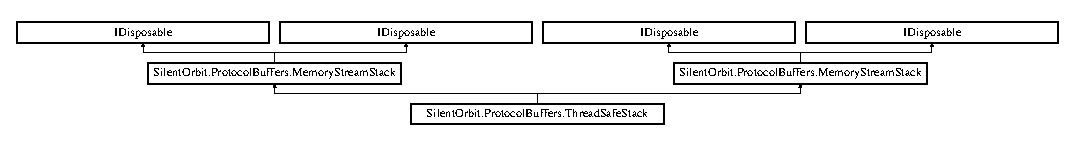
\includegraphics[height=1.443299cm]{class_silent_orbit_1_1_protocol_buffers_1_1_thread_safe_stack}
\end{center}
\end{figure}
\subsection*{Public Member Functions}
\begin{DoxyCompactItemize}
\item 
Memory\+Stream \hyperlink{class_silent_orbit_1_1_protocol_buffers_1_1_thread_safe_stack_ad9a71abbe4bf29e0aeb171ed641f5395}{Pop} ()
\begin{DoxyCompactList}\small\item\em The returned stream is not reset. You must call .Set\+Length(0) before using it. This is done in the generated code. \end{DoxyCompactList}\item 
void {\bfseries Push} (Memory\+Stream stream)\hypertarget{class_silent_orbit_1_1_protocol_buffers_1_1_thread_safe_stack_aacc42faf2152bfb517c050c0a4cd375d}{}\label{class_silent_orbit_1_1_protocol_buffers_1_1_thread_safe_stack_aacc42faf2152bfb517c050c0a4cd375d}

\item 
void {\bfseries Dispose} ()\hypertarget{class_silent_orbit_1_1_protocol_buffers_1_1_thread_safe_stack_a5b6ac8763abf573e720b546f8e53690e}{}\label{class_silent_orbit_1_1_protocol_buffers_1_1_thread_safe_stack_a5b6ac8763abf573e720b546f8e53690e}

\item 
Memory\+Stream \hyperlink{class_silent_orbit_1_1_protocol_buffers_1_1_thread_safe_stack_ad9a71abbe4bf29e0aeb171ed641f5395}{Pop} ()
\begin{DoxyCompactList}\small\item\em The returned stream is not reset. You must call .Set\+Length(0) before using it. This is done in the generated code. \end{DoxyCompactList}\item 
void {\bfseries Push} (Memory\+Stream stream)\hypertarget{class_silent_orbit_1_1_protocol_buffers_1_1_thread_safe_stack_aacc42faf2152bfb517c050c0a4cd375d}{}\label{class_silent_orbit_1_1_protocol_buffers_1_1_thread_safe_stack_aacc42faf2152bfb517c050c0a4cd375d}

\item 
void {\bfseries Dispose} ()\hypertarget{class_silent_orbit_1_1_protocol_buffers_1_1_thread_safe_stack_a5b6ac8763abf573e720b546f8e53690e}{}\label{class_silent_orbit_1_1_protocol_buffers_1_1_thread_safe_stack_a5b6ac8763abf573e720b546f8e53690e}

\end{DoxyCompactItemize}


\subsection{Detailed Description}
Thread safe stack of memory streams 



\subsection{Member Function Documentation}
\index{Silent\+Orbit\+::\+Protocol\+Buffers\+::\+Thread\+Safe\+Stack@{Silent\+Orbit\+::\+Protocol\+Buffers\+::\+Thread\+Safe\+Stack}!Pop@{Pop}}
\index{Pop@{Pop}!Silent\+Orbit\+::\+Protocol\+Buffers\+::\+Thread\+Safe\+Stack@{Silent\+Orbit\+::\+Protocol\+Buffers\+::\+Thread\+Safe\+Stack}}
\subsubsection[{\texorpdfstring{Pop()}{Pop()}}]{\setlength{\rightskip}{0pt plus 5cm}Memory\+Stream Silent\+Orbit.\+Protocol\+Buffers.\+Thread\+Safe\+Stack.\+Pop (
\begin{DoxyParamCaption}
{}
\end{DoxyParamCaption}
)\hspace{0.3cm}{\ttfamily [inline]}}\hypertarget{class_silent_orbit_1_1_protocol_buffers_1_1_thread_safe_stack_ad9a71abbe4bf29e0aeb171ed641f5395}{}\label{class_silent_orbit_1_1_protocol_buffers_1_1_thread_safe_stack_ad9a71abbe4bf29e0aeb171ed641f5395}


The returned stream is not reset. You must call .Set\+Length(0) before using it. This is done in the generated code. 



Implements \hyperlink{interface_silent_orbit_1_1_protocol_buffers_1_1_memory_stream_stack}{Silent\+Orbit.\+Protocol\+Buffers.\+Memory\+Stream\+Stack}.

\index{Silent\+Orbit\+::\+Protocol\+Buffers\+::\+Thread\+Safe\+Stack@{Silent\+Orbit\+::\+Protocol\+Buffers\+::\+Thread\+Safe\+Stack}!Pop@{Pop}}
\index{Pop@{Pop}!Silent\+Orbit\+::\+Protocol\+Buffers\+::\+Thread\+Safe\+Stack@{Silent\+Orbit\+::\+Protocol\+Buffers\+::\+Thread\+Safe\+Stack}}
\subsubsection[{\texorpdfstring{Pop()}{Pop()}}]{\setlength{\rightskip}{0pt plus 5cm}Memory\+Stream Silent\+Orbit.\+Protocol\+Buffers.\+Thread\+Safe\+Stack.\+Pop (
\begin{DoxyParamCaption}
{}
\end{DoxyParamCaption}
)\hspace{0.3cm}{\ttfamily [inline]}}\hypertarget{class_silent_orbit_1_1_protocol_buffers_1_1_thread_safe_stack_ad9a71abbe4bf29e0aeb171ed641f5395}{}\label{class_silent_orbit_1_1_protocol_buffers_1_1_thread_safe_stack_ad9a71abbe4bf29e0aeb171ed641f5395}


The returned stream is not reset. You must call .Set\+Length(0) before using it. This is done in the generated code. 



Implements \hyperlink{interface_silent_orbit_1_1_protocol_buffers_1_1_memory_stream_stack}{Silent\+Orbit.\+Protocol\+Buffers.\+Memory\+Stream\+Stack}.



The documentation for this class was generated from the following file\+:\begin{DoxyCompactItemize}
\item 
/home/andrea/\+Clion\+Projects/saas/cdti/\+C\+D\+T\+I\+Unity/\+Assets/scripts/Protocol\+Parser.\+cs\end{DoxyCompactItemize}

\hypertarget{class_silent_orbit_1_1_protocol_buffers_1_1_thread_unsafe_stack}{}\section{Silent\+Orbit.\+Protocol\+Buffers.\+Thread\+Unsafe\+Stack Class Reference}
\label{class_silent_orbit_1_1_protocol_buffers_1_1_thread_unsafe_stack}\index{Silent\+Orbit.\+Protocol\+Buffers.\+Thread\+Unsafe\+Stack@{Silent\+Orbit.\+Protocol\+Buffers.\+Thread\+Unsafe\+Stack}}


Non-\/thread safe stack of memory streams Safe as long as only one thread is Serializing  


Inheritance diagram for Silent\+Orbit.\+Protocol\+Buffers.\+Thread\+Unsafe\+Stack\+:\begin{figure}[H]
\begin{center}
\leavevmode
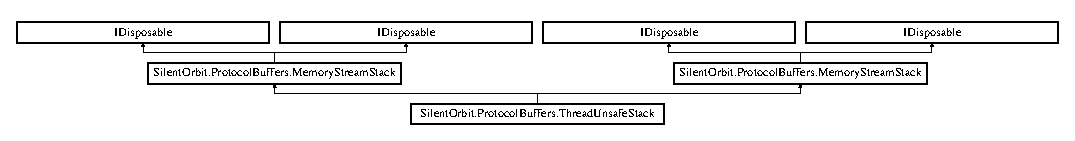
\includegraphics[height=1.443299cm]{class_silent_orbit_1_1_protocol_buffers_1_1_thread_unsafe_stack}
\end{center}
\end{figure}
\subsection*{Public Member Functions}
\begin{DoxyCompactItemize}
\item 
Memory\+Stream \hyperlink{class_silent_orbit_1_1_protocol_buffers_1_1_thread_unsafe_stack_a15e031438325f7f907c6f4c978accc9e}{Pop} ()
\begin{DoxyCompactList}\small\item\em The returned stream is not reset. You must call .Set\+Length(0) before using it. This is done in the generated code. \end{DoxyCompactList}\item 
\hypertarget{class_silent_orbit_1_1_protocol_buffers_1_1_thread_unsafe_stack_ae5b6470796f24067b996ba9afe305ae9}{}void {\bfseries Push} (Memory\+Stream stream)\label{class_silent_orbit_1_1_protocol_buffers_1_1_thread_unsafe_stack_ae5b6470796f24067b996ba9afe305ae9}

\item 
\hypertarget{class_silent_orbit_1_1_protocol_buffers_1_1_thread_unsafe_stack_ae6e46514280c99eb7b83015827cb669c}{}void {\bfseries Dispose} ()\label{class_silent_orbit_1_1_protocol_buffers_1_1_thread_unsafe_stack_ae6e46514280c99eb7b83015827cb669c}

\item 
Memory\+Stream \hyperlink{class_silent_orbit_1_1_protocol_buffers_1_1_thread_unsafe_stack_a15e031438325f7f907c6f4c978accc9e}{Pop} ()
\begin{DoxyCompactList}\small\item\em The returned stream is not reset. You must call .Set\+Length(0) before using it. This is done in the generated code. \end{DoxyCompactList}\item 
\hypertarget{class_silent_orbit_1_1_protocol_buffers_1_1_thread_unsafe_stack_ae5b6470796f24067b996ba9afe305ae9}{}void {\bfseries Push} (Memory\+Stream stream)\label{class_silent_orbit_1_1_protocol_buffers_1_1_thread_unsafe_stack_ae5b6470796f24067b996ba9afe305ae9}

\item 
\hypertarget{class_silent_orbit_1_1_protocol_buffers_1_1_thread_unsafe_stack_ae6e46514280c99eb7b83015827cb669c}{}void {\bfseries Dispose} ()\label{class_silent_orbit_1_1_protocol_buffers_1_1_thread_unsafe_stack_ae6e46514280c99eb7b83015827cb669c}

\end{DoxyCompactItemize}


\subsection{Detailed Description}
Non-\/thread safe stack of memory streams Safe as long as only one thread is Serializing 



\subsection{Member Function Documentation}
\hypertarget{class_silent_orbit_1_1_protocol_buffers_1_1_thread_unsafe_stack_a15e031438325f7f907c6f4c978accc9e}{}\index{Silent\+Orbit\+::\+Protocol\+Buffers\+::\+Thread\+Unsafe\+Stack@{Silent\+Orbit\+::\+Protocol\+Buffers\+::\+Thread\+Unsafe\+Stack}!Pop@{Pop}}
\index{Pop@{Pop}!Silent\+Orbit\+::\+Protocol\+Buffers\+::\+Thread\+Unsafe\+Stack@{Silent\+Orbit\+::\+Protocol\+Buffers\+::\+Thread\+Unsafe\+Stack}}
\subsubsection[{Pop}]{\setlength{\rightskip}{0pt plus 5cm}Memory\+Stream Silent\+Orbit.\+Protocol\+Buffers.\+Thread\+Unsafe\+Stack.\+Pop (
\begin{DoxyParamCaption}
{}
\end{DoxyParamCaption}
)\hspace{0.3cm}{\ttfamily [inline]}}\label{class_silent_orbit_1_1_protocol_buffers_1_1_thread_unsafe_stack_a15e031438325f7f907c6f4c978accc9e}


The returned stream is not reset. You must call .Set\+Length(0) before using it. This is done in the generated code. 



Implements \hyperlink{interface_silent_orbit_1_1_protocol_buffers_1_1_memory_stream_stack}{Silent\+Orbit.\+Protocol\+Buffers.\+Memory\+Stream\+Stack}.

\hypertarget{class_silent_orbit_1_1_protocol_buffers_1_1_thread_unsafe_stack_a15e031438325f7f907c6f4c978accc9e}{}\index{Silent\+Orbit\+::\+Protocol\+Buffers\+::\+Thread\+Unsafe\+Stack@{Silent\+Orbit\+::\+Protocol\+Buffers\+::\+Thread\+Unsafe\+Stack}!Pop@{Pop}}
\index{Pop@{Pop}!Silent\+Orbit\+::\+Protocol\+Buffers\+::\+Thread\+Unsafe\+Stack@{Silent\+Orbit\+::\+Protocol\+Buffers\+::\+Thread\+Unsafe\+Stack}}
\subsubsection[{Pop}]{\setlength{\rightskip}{0pt plus 5cm}Memory\+Stream Silent\+Orbit.\+Protocol\+Buffers.\+Thread\+Unsafe\+Stack.\+Pop (
\begin{DoxyParamCaption}
{}
\end{DoxyParamCaption}
)\hspace{0.3cm}{\ttfamily [inline]}}\label{class_silent_orbit_1_1_protocol_buffers_1_1_thread_unsafe_stack_a15e031438325f7f907c6f4c978accc9e}


The returned stream is not reset. You must call .Set\+Length(0) before using it. This is done in the generated code. 



Implements \hyperlink{interface_silent_orbit_1_1_protocol_buffers_1_1_memory_stream_stack}{Silent\+Orbit.\+Protocol\+Buffers.\+Memory\+Stream\+Stack}.



The documentation for this class was generated from the following file\+:\begin{DoxyCompactItemize}
\item 
/home/fpoole/development/cpe406/saas/cdti/\+C\+D\+T\+I\+Unity/\+Assets/scripts/Protocol\+Parser.\+cs\end{DoxyCompactItemize}

\hypertarget{class_json_1_1_value}{}\section{Json\+:\+:Value Class Reference}
\label{class_json_1_1_value}\index{Json\+::\+Value@{Json\+::\+Value}}


Represents a \href{http://www.json.org}{\tt J\+S\+ON} value.  




{\ttfamily \#include $<$json.\+h$>$}

\subsection*{Public Types}
\begin{DoxyCompactItemize}
\item 
typedef std\+::vector$<$ std\+::string $>$ {\bfseries Members}\hypertarget{class_json_1_1_value_ac61bab5a465848b57610379cc07995c3}{}\label{class_json_1_1_value_ac61bab5a465848b57610379cc07995c3}

\item 
typedef \hyperlink{class_json_1_1_value_iterator}{Value\+Iterator} {\bfseries iterator}\hypertarget{class_json_1_1_value_a341cdf2e01f8b3c5b7317aa2f0768c53}{}\label{class_json_1_1_value_a341cdf2e01f8b3c5b7317aa2f0768c53}

\item 
typedef \hyperlink{class_json_1_1_value_const_iterator}{Value\+Const\+Iterator} {\bfseries const\+\_\+iterator}\hypertarget{class_json_1_1_value_af92282ca92b58b320debd486afb7696a}{}\label{class_json_1_1_value_af92282ca92b58b320debd486afb7696a}

\item 
typedef Json\+::\+U\+Int {\bfseries U\+Int}\hypertarget{class_json_1_1_value_a0933d59b45793ae4aade1757c322a98d}{}\label{class_json_1_1_value_a0933d59b45793ae4aade1757c322a98d}

\item 
typedef Json\+::\+Int {\bfseries Int}\hypertarget{class_json_1_1_value_abdf7a7ff73eb130ffcab28504ffdb405}{}\label{class_json_1_1_value_abdf7a7ff73eb130ffcab28504ffdb405}

\item 
typedef Json\+::\+U\+Int64 {\bfseries U\+Int64}\hypertarget{class_json_1_1_value_a8b62564be8c087c6d18de180ff4e13e3}{}\label{class_json_1_1_value_a8b62564be8c087c6d18de180ff4e13e3}

\item 
typedef Json\+::\+Int64 {\bfseries Int64}\hypertarget{class_json_1_1_value_a1b86af9f85f0f1baa972c3319fa22695}{}\label{class_json_1_1_value_a1b86af9f85f0f1baa972c3319fa22695}

\item 
typedef Json\+::\+Largest\+Int {\bfseries Largest\+Int}\hypertarget{class_json_1_1_value_a1cbb82642ed05109b9833e49f042ece7}{}\label{class_json_1_1_value_a1cbb82642ed05109b9833e49f042ece7}

\item 
typedef Json\+::\+Largest\+U\+Int {\bfseries Largest\+U\+Int}\hypertarget{class_json_1_1_value_a6682a3684d635e03fc06ba229fa24eec}{}\label{class_json_1_1_value_a6682a3684d635e03fc06ba229fa24eec}

\item 
typedef Json\+::\+Array\+Index {\bfseries Array\+Index}\hypertarget{class_json_1_1_value_a184a91566cccca7b819240f0d5561c7d}{}\label{class_json_1_1_value_a184a91566cccca7b819240f0d5561c7d}

\item 
typedef std\+::map$<$ C\+Z\+String, \hyperlink{class_json_1_1_value}{Value} $>$ {\bfseries Object\+Values}\hypertarget{class_json_1_1_value_a08b6c80c3af7071d908dabf044de5388}{}\label{class_json_1_1_value_a08b6c80c3af7071d908dabf044de5388}

\end{DoxyCompactItemize}
\subsection*{Public Member Functions}
\begin{DoxyCompactItemize}
\item 
\hyperlink{class_json_1_1_value_ada6ba1369448fb0240bccc36efaa46f7}{Value} (\hyperlink{namespace_json_a7d654b75c16a57007925868e38212b4e}{Value\+Type} type=\hyperlink{namespace_json_a7d654b75c16a57007925868e38212b4ea7d9899633b4409bd3fc107e6737f8391}{null\+Value})
\begin{DoxyCompactList}\small\item\em Create a default \hyperlink{class_json_1_1_value}{Value} of the given type. \end{DoxyCompactList}\item 
{\bfseries Value} (Int value)\hypertarget{class_json_1_1_value_a4744ae571fcf34f4b16a2257b3b3b585}{}\label{class_json_1_1_value_a4744ae571fcf34f4b16a2257b3b3b585}

\item 
{\bfseries Value} (U\+Int value)\hypertarget{class_json_1_1_value_ae67a857b01286e3499a87e95be848d20}{}\label{class_json_1_1_value_ae67a857b01286e3499a87e95be848d20}

\item 
{\bfseries Value} (Int64 value)\hypertarget{class_json_1_1_value_ab1cdc3d9a4d4cc03fa01439d43ceb1b5}{}\label{class_json_1_1_value_ab1cdc3d9a4d4cc03fa01439d43ceb1b5}

\item 
{\bfseries Value} (U\+Int64 value)\hypertarget{class_json_1_1_value_a8adda58d5ae17bf7ca6a53bab4a7b69c}{}\label{class_json_1_1_value_a8adda58d5ae17bf7ca6a53bab4a7b69c}

\item 
{\bfseries Value} (double value)\hypertarget{class_json_1_1_value_a32228cc84d83200cca8441451997996c}{}\label{class_json_1_1_value_a32228cc84d83200cca8441451997996c}

\item 
\hyperlink{class_json_1_1_value_ad87b849356816aca75995dd07302e49d}{Value} (const char $\ast$value)\hypertarget{class_json_1_1_value_ad87b849356816aca75995dd07302e49d}{}\label{class_json_1_1_value_ad87b849356816aca75995dd07302e49d}

\begin{DoxyCompactList}\small\item\em Copy til first 0. (N\+U\+LL causes to seg-\/fault.) \end{DoxyCompactList}\item 
\hyperlink{class_json_1_1_value_a39fa09d1902efbd4350e1236db920571}{Value} (const char $\ast$begin, const char $\ast$end)\hypertarget{class_json_1_1_value_a39fa09d1902efbd4350e1236db920571}{}\label{class_json_1_1_value_a39fa09d1902efbd4350e1236db920571}

\begin{DoxyCompactList}\small\item\em Copy all, incl zeroes. \end{DoxyCompactList}\item 
\hyperlink{class_json_1_1_value_a081830e95f88a37054da7e46c65b0766}{Value} (const \hyperlink{class_json_1_1_static_string}{Static\+String} \&value)
\begin{DoxyCompactList}\small\item\em Constructs a value from a static string. \end{DoxyCompactList}\item 
\hyperlink{class_json_1_1_value_aa4501dd4edf3ce3d5145fc656f088b21}{Value} (const std\+::string \&value)\hypertarget{class_json_1_1_value_aa4501dd4edf3ce3d5145fc656f088b21}{}\label{class_json_1_1_value_aa4501dd4edf3ce3d5145fc656f088b21}

\begin{DoxyCompactList}\small\item\em Copy data() til \hyperlink{class_json_1_1_value_a4ca8ee6c48a34ca6c2f131956bab5e05}{size()}. Embedded zeroes too. \end{DoxyCompactList}\item 
{\bfseries Value} (bool value)\hypertarget{class_json_1_1_value_a350a31ea4a30d384994b0bc010b17495}{}\label{class_json_1_1_value_a350a31ea4a30d384994b0bc010b17495}

\item 
\hyperlink{class_json_1_1_value_a436dfd3670f95fd665f680eba5cebcf0}{Value} (const \hyperlink{class_json_1_1_value}{Value} \&other)\hypertarget{class_json_1_1_value_a436dfd3670f95fd665f680eba5cebcf0}{}\label{class_json_1_1_value_a436dfd3670f95fd665f680eba5cebcf0}

\begin{DoxyCompactList}\small\item\em Deep copy. \end{DoxyCompactList}\item 
\hyperlink{class_json_1_1_value}{Value} \& \hyperlink{class_json_1_1_value_a795acb28772da4c5d85ae8f4af36c69f}{operator=} (\hyperlink{class_json_1_1_value}{Value} other)
\item 
void \hyperlink{class_json_1_1_value_aab841120d78e296e1bc06a373345e822}{swap} (\hyperlink{class_json_1_1_value}{Value} \&other)\hypertarget{class_json_1_1_value_aab841120d78e296e1bc06a373345e822}{}\label{class_json_1_1_value_aab841120d78e296e1bc06a373345e822}

\begin{DoxyCompactList}\small\item\em Swap everything. \end{DoxyCompactList}\item 
void \hyperlink{class_json_1_1_value_a5263476047f20e2fc6de470e4de34fe5}{swap\+Payload} (\hyperlink{class_json_1_1_value}{Value} \&other)\hypertarget{class_json_1_1_value_a5263476047f20e2fc6de470e4de34fe5}{}\label{class_json_1_1_value_a5263476047f20e2fc6de470e4de34fe5}

\begin{DoxyCompactList}\small\item\em Swap values but leave comments and source offsets in place. \end{DoxyCompactList}\item 
\hyperlink{namespace_json_a7d654b75c16a57007925868e38212b4e}{Value\+Type} {\bfseries type} () const \hypertarget{class_json_1_1_value_a695ef31fad36b4712918b3ff80158479}{}\label{class_json_1_1_value_a695ef31fad36b4712918b3ff80158479}

\item 
bool \hyperlink{class_json_1_1_value_af0ad8aa027575c3277296458f3fb7b0a}{operator$<$} (const \hyperlink{class_json_1_1_value}{Value} \&other) const \hypertarget{class_json_1_1_value_af0ad8aa027575c3277296458f3fb7b0a}{}\label{class_json_1_1_value_af0ad8aa027575c3277296458f3fb7b0a}

\begin{DoxyCompactList}\small\item\em Compare payload only, not comments etc. \end{DoxyCompactList}\item 
bool {\bfseries operator$<$=} (const \hyperlink{class_json_1_1_value}{Value} \&other) const \hypertarget{class_json_1_1_value_afb99dd3628fe44244b32007f9b4f369a}{}\label{class_json_1_1_value_afb99dd3628fe44244b32007f9b4f369a}

\item 
bool {\bfseries operator$>$=} (const \hyperlink{class_json_1_1_value}{Value} \&other) const \hypertarget{class_json_1_1_value_acc13fc47d55abd6e2327b090b83d2911}{}\label{class_json_1_1_value_acc13fc47d55abd6e2327b090b83d2911}

\item 
bool {\bfseries operator$>$} (const \hyperlink{class_json_1_1_value}{Value} \&other) const \hypertarget{class_json_1_1_value_a3124a26067bdfde9571bc89527fc6931}{}\label{class_json_1_1_value_a3124a26067bdfde9571bc89527fc6931}

\item 
bool {\bfseries operator==} (const \hyperlink{class_json_1_1_value}{Value} \&other) const \hypertarget{class_json_1_1_value_a14363dda23a6ae2def9afd1590ae85d3}{}\label{class_json_1_1_value_a14363dda23a6ae2def9afd1590ae85d3}

\item 
bool {\bfseries operator!=} (const \hyperlink{class_json_1_1_value}{Value} \&other) const \hypertarget{class_json_1_1_value_ad0f12d2a4ab74bbef08a05504b2cb81d}{}\label{class_json_1_1_value_ad0f12d2a4ab74bbef08a05504b2cb81d}

\item 
int {\bfseries compare} (const \hyperlink{class_json_1_1_value}{Value} \&other) const \hypertarget{class_json_1_1_value_a899214ed2253d3f4f061b922b0e622b5}{}\label{class_json_1_1_value_a899214ed2253d3f4f061b922b0e622b5}

\item 
const char $\ast$ \hyperlink{class_json_1_1_value_a5b7da48b163bcec63b1424f1608b7da6}{as\+C\+String} () const \hypertarget{class_json_1_1_value_a5b7da48b163bcec63b1424f1608b7da6}{}\label{class_json_1_1_value_a5b7da48b163bcec63b1424f1608b7da6}

\begin{DoxyCompactList}\small\item\em Embedded zeroes could cause you trouble! \end{DoxyCompactList}\item 
std\+::string \hyperlink{class_json_1_1_value_a03ee3d5df576640c93ba683f140828bd}{as\+String} () const \hypertarget{class_json_1_1_value_a03ee3d5df576640c93ba683f140828bd}{}\label{class_json_1_1_value_a03ee3d5df576640c93ba683f140828bd}

\begin{DoxyCompactList}\small\item\em Embedded zeroes are possible. \end{DoxyCompactList}\item 
bool \hyperlink{class_json_1_1_value_a1e0263113ae247a632afac43ebc4149f}{get\+String} (char const $\ast$$\ast$begin, char const $\ast$$\ast$end) const 
\item 
Int {\bfseries as\+Int} () const \hypertarget{class_json_1_1_value_ac786e35b860b1d700cb3d3e56dd6a235}{}\label{class_json_1_1_value_ac786e35b860b1d700cb3d3e56dd6a235}

\item 
U\+Int {\bfseries as\+U\+Int} () const \hypertarget{class_json_1_1_value_a2019d1bd296b89356c1b0da5970c918c}{}\label{class_json_1_1_value_a2019d1bd296b89356c1b0da5970c918c}

\item 
Int64 {\bfseries as\+Int64} () const \hypertarget{class_json_1_1_value_a4451cee7524534458894f4e2cc045aa3}{}\label{class_json_1_1_value_a4451cee7524534458894f4e2cc045aa3}

\item 
U\+Int64 {\bfseries as\+U\+Int64} () const \hypertarget{class_json_1_1_value_a4aa617bc0625ae0f208fa54b7c6326ad}{}\label{class_json_1_1_value_a4aa617bc0625ae0f208fa54b7c6326ad}

\item 
Largest\+Int {\bfseries as\+Largest\+Int} () const \hypertarget{class_json_1_1_value_a3786bb100c5cf9a98eb6d13784968956}{}\label{class_json_1_1_value_a3786bb100c5cf9a98eb6d13784968956}

\item 
Largest\+U\+Int {\bfseries as\+Largest\+U\+Int} () const \hypertarget{class_json_1_1_value_a692b88345a745b2f89ca5d94b52e94d4}{}\label{class_json_1_1_value_a692b88345a745b2f89ca5d94b52e94d4}

\item 
float {\bfseries as\+Float} () const \hypertarget{class_json_1_1_value_ac2128d7080499daf8c5b1c71da243f63}{}\label{class_json_1_1_value_ac2128d7080499daf8c5b1c71da243f63}

\item 
double {\bfseries as\+Double} () const \hypertarget{class_json_1_1_value_a33434ed1c0217a34d04c95fa5342fd37}{}\label{class_json_1_1_value_a33434ed1c0217a34d04c95fa5342fd37}

\item 
bool {\bfseries as\+Bool} () const \hypertarget{class_json_1_1_value_a7402c797285c020566c3db5f8ae4e940}{}\label{class_json_1_1_value_a7402c797285c020566c3db5f8ae4e940}

\item 
bool {\bfseries is\+Null} () const \hypertarget{class_json_1_1_value_aeb9ad8b1bb91bdd72203dc884b3f4362}{}\label{class_json_1_1_value_aeb9ad8b1bb91bdd72203dc884b3f4362}

\item 
bool {\bfseries is\+Bool} () const \hypertarget{class_json_1_1_value_a3c3716cc7a0216cb1b654bb8f61c8d13}{}\label{class_json_1_1_value_a3c3716cc7a0216cb1b654bb8f61c8d13}

\item 
bool {\bfseries is\+Int} () const \hypertarget{class_json_1_1_value_ab0df4746d6787d2ce1db1a156c118f14}{}\label{class_json_1_1_value_ab0df4746d6787d2ce1db1a156c118f14}

\item 
bool {\bfseries is\+Int64} () const \hypertarget{class_json_1_1_value_aba89690e5fd72d0f7121a30013470423}{}\label{class_json_1_1_value_aba89690e5fd72d0f7121a30013470423}

\item 
bool {\bfseries is\+U\+Int} () const \hypertarget{class_json_1_1_value_ae814ca1796fe2d43ac09898b70213989}{}\label{class_json_1_1_value_ae814ca1796fe2d43ac09898b70213989}

\item 
bool {\bfseries is\+U\+Int64} () const \hypertarget{class_json_1_1_value_aa35efece2a6cba4d988d7d5b54db2fb8}{}\label{class_json_1_1_value_aa35efece2a6cba4d988d7d5b54db2fb8}

\item 
bool {\bfseries is\+Integral} () const \hypertarget{class_json_1_1_value_aec4f74ef7b776b1d9c8a10fc3bb4add5}{}\label{class_json_1_1_value_aec4f74ef7b776b1d9c8a10fc3bb4add5}

\item 
bool {\bfseries is\+Double} () const \hypertarget{class_json_1_1_value_a0ea567fa51fc808851698bef59b43626}{}\label{class_json_1_1_value_a0ea567fa51fc808851698bef59b43626}

\item 
bool {\bfseries is\+Numeric} () const \hypertarget{class_json_1_1_value_a8ce848900e2e8fa23a41fcc2c1409fab}{}\label{class_json_1_1_value_a8ce848900e2e8fa23a41fcc2c1409fab}

\item 
bool {\bfseries is\+String} () const \hypertarget{class_json_1_1_value_a06c01d7c1e8151a5844b595ab00f46c7}{}\label{class_json_1_1_value_a06c01d7c1e8151a5844b595ab00f46c7}

\item 
bool {\bfseries is\+Array} () const \hypertarget{class_json_1_1_value_ac8c898f93543e55b67418f94bced20af}{}\label{class_json_1_1_value_ac8c898f93543e55b67418f94bced20af}

\item 
bool {\bfseries is\+Object} () const \hypertarget{class_json_1_1_value_a80cffaa0402b80317c0437216bbb6d92}{}\label{class_json_1_1_value_a80cffaa0402b80317c0437216bbb6d92}

\item 
bool {\bfseries is\+Convertible\+To} (\hyperlink{namespace_json_a7d654b75c16a57007925868e38212b4e}{Value\+Type} other) const \hypertarget{class_json_1_1_value_a7ec153803631a27abf58cba2bb1af70c}{}\label{class_json_1_1_value_a7ec153803631a27abf58cba2bb1af70c}

\item 
Array\+Index \hyperlink{class_json_1_1_value_a4ca8ee6c48a34ca6c2f131956bab5e05}{size} () const \hypertarget{class_json_1_1_value_a4ca8ee6c48a34ca6c2f131956bab5e05}{}\label{class_json_1_1_value_a4ca8ee6c48a34ca6c2f131956bab5e05}

\begin{DoxyCompactList}\small\item\em Number of values in array or object. \end{DoxyCompactList}\item 
bool \hyperlink{class_json_1_1_value_a99c42d3ff8495dad1e91b43e66553c36}{empty} () const \hypertarget{class_json_1_1_value_a99c42d3ff8495dad1e91b43e66553c36}{}\label{class_json_1_1_value_a99c42d3ff8495dad1e91b43e66553c36}

\begin{DoxyCompactList}\small\item\em Return true if empty array, empty object, or null; otherwise, false. \end{DoxyCompactList}\item 
bool \hyperlink{class_json_1_1_value_a021ab0d15a807fbe051446c9c545ab61}{operator!} () const \hypertarget{class_json_1_1_value_a021ab0d15a807fbe051446c9c545ab61}{}\label{class_json_1_1_value_a021ab0d15a807fbe051446c9c545ab61}

\begin{DoxyCompactList}\small\item\em Return is\+Null() \end{DoxyCompactList}\item 
void \hyperlink{class_json_1_1_value_a501a4d67e6c875255c2ecc03ccd2019b}{clear} ()
\item 
void \hyperlink{class_json_1_1_value_aa284353271ada427dbfa04a42f2be407}{resize} (Array\+Index \hyperlink{class_json_1_1_value_a4ca8ee6c48a34ca6c2f131956bab5e05}{size})
\item 
\hyperlink{class_json_1_1_value}{Value} \& \hyperlink{class_json_1_1_value_a7d99f5dba388cdaa152ce6ef933d64ef}{operator\mbox{[}$\,$\mbox{]}} (Array\+Index index)
\item 
\hyperlink{class_json_1_1_value}{Value} \& \hyperlink{class_json_1_1_value_ac9182982c361e0ab621134d406e5f250}{operator\mbox{[}$\,$\mbox{]}} (int index)
\item 
const \hyperlink{class_json_1_1_value}{Value} \& \hyperlink{class_json_1_1_value_af151919e8947c430e34bed2b0b128601}{operator\mbox{[}$\,$\mbox{]}} (Array\+Index index) const 
\item 
const \hyperlink{class_json_1_1_value}{Value} \& \hyperlink{class_json_1_1_value_af9e02b38f4e63e491c300c20b275bdd7}{operator\mbox{[}$\,$\mbox{]}} (int index) const 
\item 
\hyperlink{class_json_1_1_value}{Value} \hyperlink{class_json_1_1_value_a28282c9b76fa031eba7a1843c47c16fe}{get} (Array\+Index index, const \hyperlink{class_json_1_1_value}{Value} \&default\+Value) const 
\item 
bool \hyperlink{class_json_1_1_value_aaa82ebb4b730ea1567d310874f47d147}{is\+Valid\+Index} (Array\+Index index) const \hypertarget{class_json_1_1_value_aaa82ebb4b730ea1567d310874f47d147}{}\label{class_json_1_1_value_aaa82ebb4b730ea1567d310874f47d147}

\begin{DoxyCompactList}\small\item\em Return true if index $<$ \hyperlink{class_json_1_1_value_a4ca8ee6c48a34ca6c2f131956bab5e05}{size()}. \end{DoxyCompactList}\item 
\hyperlink{class_json_1_1_value}{Value} \& \hyperlink{class_json_1_1_value_a7e49ac977e4bcf59745a09d426669f75}{append} (const \hyperlink{class_json_1_1_value}{Value} \&value)
\begin{DoxyCompactList}\small\item\em Append value to array at the end. \end{DoxyCompactList}\item 
\hyperlink{class_json_1_1_value}{Value} \& \hyperlink{class_json_1_1_value_acb912f4ec40a25ea6eb387730885f3d9}{operator\mbox{[}$\,$\mbox{]}} (const char $\ast$key)
\item 
const \hyperlink{class_json_1_1_value}{Value} \& \hyperlink{class_json_1_1_value_ae5f73ffc7a039bca81b7ca771bc5db55}{operator\mbox{[}$\,$\mbox{]}} (const char $\ast$key) const 
\item 
\hyperlink{class_json_1_1_value}{Value} \& \hyperlink{class_json_1_1_value_ae511c7d46bf457412fb55c9471af9f50}{operator\mbox{[}$\,$\mbox{]}} (const std\+::string \&key)
\item 
const \hyperlink{class_json_1_1_value}{Value} \& \hyperlink{class_json_1_1_value_a3c53bfd2381d5a61036d7dc0b023d697}{operator\mbox{[}$\,$\mbox{]}} (const std\+::string \&key) const 
\item 
\hyperlink{class_json_1_1_value}{Value} \& \hyperlink{class_json_1_1_value_ac3763d7d315ca65dc188e273722f7955}{operator\mbox{[}$\,$\mbox{]}} (const \hyperlink{class_json_1_1_static_string}{Static\+String} \&key)
\begin{DoxyCompactList}\small\item\em Access an object value by name, create a null member if it does not exist. \end{DoxyCompactList}\item 
\hyperlink{class_json_1_1_value}{Value} \hyperlink{class_json_1_1_value_ab76b3323cde14c7db20676d07b260ce7}{get} (const char $\ast$key, const \hyperlink{class_json_1_1_value}{Value} \&default\+Value) const 
\item 
\hyperlink{class_json_1_1_value}{Value} \hyperlink{class_json_1_1_value_abcb2289c005bc0befdedaa94f662f63f}{get} (const char $\ast$begin, const char $\ast$end, const \hyperlink{class_json_1_1_value}{Value} \&default\+Value) const 
\item 
\hyperlink{class_json_1_1_value}{Value} \hyperlink{class_json_1_1_value_a54a34264356e01ee9c21a75ccfc809e9}{get} (const std\+::string \&key, const \hyperlink{class_json_1_1_value}{Value} \&default\+Value) const 
\item 
\hyperlink{class_json_1_1_value}{Value} const $\ast$ \hyperlink{class_json_1_1_value_a184bf49ec5da7ec31af089cf6f458f99}{find} (char const $\ast$begin, char const $\ast$end) const 
\item 
\hyperlink{class_json_1_1_value}{Value} const $\ast$ \hyperlink{class_json_1_1_value_afeb7ff596a0929d90c5f2f3cffb413ed}{demand} (char const $\ast$begin, char const $\ast$end)
\item 
\hyperlink{class_json_1_1_value}{Value} \hyperlink{class_json_1_1_value_aa52f7873b95d29627d6e83ba96f69aaa}{remove\+Member} (const char $\ast$key)
\begin{DoxyCompactList}\small\item\em Remove and return the named member. \end{DoxyCompactList}\item 
\hyperlink{class_json_1_1_value}{Value} \hyperlink{class_json_1_1_value_ae1f95f7ca3906e6bcc2a7be93210ecba}{remove\+Member} (const std\+::string \&key)
\item 
bool \hyperlink{class_json_1_1_value_a708e599489adf30d65bf85a8ee16e6fb}{remove\+Member} (const char $\ast$key, \hyperlink{class_json_1_1_value}{Value} $\ast$removed)
\item 
bool \hyperlink{class_json_1_1_value_a3749dae413a73eac05b7f8dc6deeb6a2}{remove\+Member} (std\+::string const \&key, \hyperlink{class_json_1_1_value}{Value} $\ast$removed)
\begin{DoxyCompactList}\small\item\em Remove the named map member. \end{DoxyCompactList}\item 
bool \hyperlink{class_json_1_1_value_a49c91af727d6b4eb0af02a81bb2def87}{remove\+Member} (const char $\ast$begin, const char $\ast$end, \hyperlink{class_json_1_1_value}{Value} $\ast$removed)\hypertarget{class_json_1_1_value_a49c91af727d6b4eb0af02a81bb2def87}{}\label{class_json_1_1_value_a49c91af727d6b4eb0af02a81bb2def87}

\begin{DoxyCompactList}\small\item\em Same as \hyperlink{class_json_1_1_value_a3749dae413a73eac05b7f8dc6deeb6a2}{remove\+Member(std\+::string const\& key, Value$\ast$ removed)} \end{DoxyCompactList}\item 
bool \hyperlink{class_json_1_1_value_ae9e67e08a85a2f3be3396ec0f4c47f65}{remove\+Index} (Array\+Index i, \hyperlink{class_json_1_1_value}{Value} $\ast$removed)
\begin{DoxyCompactList}\small\item\em Remove the indexed array element. \end{DoxyCompactList}\item 
bool \hyperlink{class_json_1_1_value_a196defba501d70ea2b6793afb04108e3}{is\+Member} (const char $\ast$key) const 
\item 
bool \hyperlink{class_json_1_1_value_af728b5738aaa133f3aad2e39dc4f415e}{is\+Member} (const std\+::string \&key) const 
\item 
bool \hyperlink{class_json_1_1_value_a077604b87a79d75543a1b5438eb9d8ab}{is\+Member} (const char $\ast$begin, const char $\ast$end) const \hypertarget{class_json_1_1_value_a077604b87a79d75543a1b5438eb9d8ab}{}\label{class_json_1_1_value_a077604b87a79d75543a1b5438eb9d8ab}

\begin{DoxyCompactList}\small\item\em Same as is\+Member(std\+::string const\& key)const. \end{DoxyCompactList}\item 
Members \hyperlink{class_json_1_1_value_a30fa08af88f2d0a038b22ba9f4e88b2a}{get\+Member\+Names} () const 
\begin{DoxyCompactList}\small\item\em Return a list of the member names. \end{DoxyCompactList}\item 
void \hyperlink{class_json_1_1_value_a29f3a30f7e5d3af6f38d57999bf5b480}{set\+Comment} (const char $\ast$comment, \hyperlink{namespace_json_a4fc417c23905b2ae9e2c47d197a45351}{Comment\+Placement} placement)
\item 
void \hyperlink{class_json_1_1_value_a2900152a2887b410a9ddabe278b9d492}{set\+Comment} (const char $\ast$comment, size\+\_\+t len, \hyperlink{namespace_json_a4fc417c23905b2ae9e2c47d197a45351}{Comment\+Placement} placement)\hypertarget{class_json_1_1_value_a2900152a2887b410a9ddabe278b9d492}{}\label{class_json_1_1_value_a2900152a2887b410a9ddabe278b9d492}

\begin{DoxyCompactList}\small\item\em Comments must be //... or /$\ast$ ... $\ast$/. \end{DoxyCompactList}\item 
void \hyperlink{class_json_1_1_value_a6d68a2e7d4e1e317cd9e812e12181689}{set\+Comment} (const std\+::string \&comment, \hyperlink{namespace_json_a4fc417c23905b2ae9e2c47d197a45351}{Comment\+Placement} placement)\hypertarget{class_json_1_1_value_a6d68a2e7d4e1e317cd9e812e12181689}{}\label{class_json_1_1_value_a6d68a2e7d4e1e317cd9e812e12181689}

\begin{DoxyCompactList}\small\item\em Comments must be //... or /$\ast$ ... $\ast$/. \end{DoxyCompactList}\item 
bool {\bfseries has\+Comment} (\hyperlink{namespace_json_a4fc417c23905b2ae9e2c47d197a45351}{Comment\+Placement} placement) const \hypertarget{class_json_1_1_value_a06567a00363cab9601be7e31336db03a}{}\label{class_json_1_1_value_a06567a00363cab9601be7e31336db03a}

\item 
std\+::string \hyperlink{class_json_1_1_value_aa1e105b5d7f55d6e42f4fb2f3674116f}{get\+Comment} (\hyperlink{namespace_json_a4fc417c23905b2ae9e2c47d197a45351}{Comment\+Placement} placement) const \hypertarget{class_json_1_1_value_aa1e105b5d7f55d6e42f4fb2f3674116f}{}\label{class_json_1_1_value_aa1e105b5d7f55d6e42f4fb2f3674116f}

\begin{DoxyCompactList}\small\item\em Include delimiters and embedded newlines. \end{DoxyCompactList}\item 
std\+::string {\bfseries to\+Styled\+String} () const \hypertarget{class_json_1_1_value_a05357cf78959b790337fae4e5580ee4f}{}\label{class_json_1_1_value_a05357cf78959b790337fae4e5580ee4f}

\item 
\hyperlink{class_json_1_1_value_const_iterator}{const\+\_\+iterator} {\bfseries begin} () const \hypertarget{class_json_1_1_value_ac12df0d6980600c5bac908ed0f64856e}{}\label{class_json_1_1_value_ac12df0d6980600c5bac908ed0f64856e}

\item 
\hyperlink{class_json_1_1_value_const_iterator}{const\+\_\+iterator} {\bfseries end} () const \hypertarget{class_json_1_1_value_a596da1926b2f2a4056bff2edb713eb0b}{}\label{class_json_1_1_value_a596da1926b2f2a4056bff2edb713eb0b}

\item 
\hyperlink{class_json_1_1_value_iterator}{iterator} {\bfseries begin} ()\hypertarget{class_json_1_1_value_a2d45bb2e68e8f22fe356d7d955ebd3c9}{}\label{class_json_1_1_value_a2d45bb2e68e8f22fe356d7d955ebd3c9}

\item 
\hyperlink{class_json_1_1_value_iterator}{iterator} {\bfseries end} ()\hypertarget{class_json_1_1_value_a2f961eff73f7f79cd29260b6cbd42558}{}\label{class_json_1_1_value_a2f961eff73f7f79cd29260b6cbd42558}

\item 
void {\bfseries set\+Offset\+Start} (size\+\_\+t start)\hypertarget{class_json_1_1_value_a6d741407c3d784360c200f181b0d6d64}{}\label{class_json_1_1_value_a6d741407c3d784360c200f181b0d6d64}

\item 
void {\bfseries set\+Offset\+Limit} (size\+\_\+t limit)\hypertarget{class_json_1_1_value_ac6d858b5fd4d5fe6ca84f697def8c5ea}{}\label{class_json_1_1_value_ac6d858b5fd4d5fe6ca84f697def8c5ea}

\item 
size\+\_\+t {\bfseries get\+Offset\+Start} () const \hypertarget{class_json_1_1_value_a10142eda11ae0b1caecbcc9f436854d1}{}\label{class_json_1_1_value_a10142eda11ae0b1caecbcc9f436854d1}

\item 
size\+\_\+t {\bfseries get\+Offset\+Limit} () const \hypertarget{class_json_1_1_value_acd7114469bc39368e9d93c29b54d8c8f}{}\label{class_json_1_1_value_acd7114469bc39368e9d93c29b54d8c8f}

\end{DoxyCompactItemize}
\subsection*{Static Public Attributes}
\begin{DoxyCompactItemize}
\item 
static const \hyperlink{class_json_1_1_value}{Value} \& \hyperlink{class_json_1_1_value_a6d6e9ea6807e46d5b7ded66d3032f607}{null} = reinterpret\+\_\+cast$<$const \hyperlink{class_json_1_1_value}{Value}\&$>$(k\+Null\+Ref)\hypertarget{class_json_1_1_value_a6d6e9ea6807e46d5b7ded66d3032f607}{}\label{class_json_1_1_value_a6d6e9ea6807e46d5b7ded66d3032f607}

\begin{DoxyCompactList}\small\item\em We regret this reference to a global instance; prefer the simpler \hyperlink{class_json_1_1_value_ada6ba1369448fb0240bccc36efaa46f7}{Value()}. \end{DoxyCompactList}\item 
static const \hyperlink{class_json_1_1_value}{Value} \& \hyperlink{class_json_1_1_value_aaa4ffd4e53967170c3e8c9abf682b5cd}{null\+Ref} = \hyperlink{class_json_1_1_value_a6d6e9ea6807e46d5b7ded66d3032f607}{null}
\item 
static const Largest\+Int \hyperlink{class_json_1_1_value_af91df130daa50dd43d2cd89e6ee67706}{min\+Largest\+Int} = Largest\+Int($\sim$(Largest\+U\+Int(-\/1) / 2))\hypertarget{class_json_1_1_value_af91df130daa50dd43d2cd89e6ee67706}{}\label{class_json_1_1_value_af91df130daa50dd43d2cd89e6ee67706}

\begin{DoxyCompactList}\small\item\em Minimum signed integer value that can be stored in a \hyperlink{class_json_1_1_value}{Json\+::\+Value}. \end{DoxyCompactList}\item 
static const Largest\+Int \hyperlink{class_json_1_1_value_a8b4977696f13296fa8755c7953fafb2f}{max\+Largest\+Int} = Largest\+Int(Largest\+U\+Int(-\/1) / 2)\hypertarget{class_json_1_1_value_a8b4977696f13296fa8755c7953fafb2f}{}\label{class_json_1_1_value_a8b4977696f13296fa8755c7953fafb2f}

\begin{DoxyCompactList}\small\item\em Maximum signed integer value that can be stored in a \hyperlink{class_json_1_1_value}{Json\+::\+Value}. \end{DoxyCompactList}\item 
static const Largest\+U\+Int \hyperlink{class_json_1_1_value_a8ddb32d9d55fa5323ae5135639dc2e31}{max\+Largest\+U\+Int} = Largest\+U\+Int(-\/1)\hypertarget{class_json_1_1_value_a8ddb32d9d55fa5323ae5135639dc2e31}{}\label{class_json_1_1_value_a8ddb32d9d55fa5323ae5135639dc2e31}

\begin{DoxyCompactList}\small\item\em Maximum unsigned integer value that can be stored in a \hyperlink{class_json_1_1_value}{Json\+::\+Value}. \end{DoxyCompactList}\item 
static const Int \hyperlink{class_json_1_1_value_a7df8a39e2502b8c92a6a41e3d752d2c8}{min\+Int} = Int($\sim$(U\+Int(-\/1) / 2))\hypertarget{class_json_1_1_value_a7df8a39e2502b8c92a6a41e3d752d2c8}{}\label{class_json_1_1_value_a7df8a39e2502b8c92a6a41e3d752d2c8}

\begin{DoxyCompactList}\small\item\em Minimum signed int value that can be stored in a \hyperlink{class_json_1_1_value}{Json\+::\+Value}. \end{DoxyCompactList}\item 
static const Int \hyperlink{class_json_1_1_value_a978c799a8af3114ef7dab6fd0a310a1b}{max\+Int} = Int(U\+Int(-\/1) / 2)\hypertarget{class_json_1_1_value_a978c799a8af3114ef7dab6fd0a310a1b}{}\label{class_json_1_1_value_a978c799a8af3114ef7dab6fd0a310a1b}

\begin{DoxyCompactList}\small\item\em Maximum signed int value that can be stored in a \hyperlink{class_json_1_1_value}{Json\+::\+Value}. \end{DoxyCompactList}\item 
static const U\+Int \hyperlink{class_json_1_1_value_ac79e63ee68d3aa914bfd6988be669b87}{max\+U\+Int} = U\+Int(-\/1)\hypertarget{class_json_1_1_value_ac79e63ee68d3aa914bfd6988be669b87}{}\label{class_json_1_1_value_ac79e63ee68d3aa914bfd6988be669b87}

\begin{DoxyCompactList}\small\item\em Maximum unsigned int value that can be stored in a \hyperlink{class_json_1_1_value}{Json\+::\+Value}. \end{DoxyCompactList}\item 
static const Int64 \hyperlink{class_json_1_1_value_a815ef899bc312c93bc426511acfe31a7}{min\+Int64}\hypertarget{class_json_1_1_value_a815ef899bc312c93bc426511acfe31a7}{}\label{class_json_1_1_value_a815ef899bc312c93bc426511acfe31a7}

\begin{DoxyCompactList}\small\item\em Minimum signed 64 bits int value that can be stored in a \hyperlink{class_json_1_1_value}{Json\+::\+Value}. \end{DoxyCompactList}\item 
static const Int64 \hyperlink{class_json_1_1_value_a4492634870b8c5709ce967b384ac6006}{max\+Int64}\hypertarget{class_json_1_1_value_a4492634870b8c5709ce967b384ac6006}{}\label{class_json_1_1_value_a4492634870b8c5709ce967b384ac6006}

\begin{DoxyCompactList}\small\item\em Maximum signed 64 bits int value that can be stored in a \hyperlink{class_json_1_1_value}{Json\+::\+Value}. \end{DoxyCompactList}\item 
static const U\+Int64 \hyperlink{class_json_1_1_value_ae1eb89c305c39516696ff305cffa01da}{max\+U\+Int64}\hypertarget{class_json_1_1_value_ae1eb89c305c39516696ff305cffa01da}{}\label{class_json_1_1_value_ae1eb89c305c39516696ff305cffa01da}

\begin{DoxyCompactList}\small\item\em Maximum unsigned 64 bits int value that can be stored in a \hyperlink{class_json_1_1_value}{Json\+::\+Value}. \end{DoxyCompactList}\end{DoxyCompactItemize}
\subsection*{Friends}
\begin{DoxyCompactItemize}
\item 
class {\bfseries Value\+Iterator\+Base}\hypertarget{class_json_1_1_value_ad016df56489e5d360735457afba2f649}{}\label{class_json_1_1_value_ad016df56489e5d360735457afba2f649}

\end{DoxyCompactItemize}


\subsection{Detailed Description}
Represents a \href{http://www.json.org}{\tt J\+S\+ON} value. 

This class is a discriminated union wrapper that can represents a\+:
\begin{DoxyItemize}
\item signed integer \mbox{[}range\+: \hyperlink{class_json_1_1_value_a7df8a39e2502b8c92a6a41e3d752d2c8}{Value\+::min\+Int} -\/ \hyperlink{class_json_1_1_value_a978c799a8af3114ef7dab6fd0a310a1b}{Value\+::max\+Int}\mbox{]}
\item unsigned integer (range\+: 0 -\/ \hyperlink{class_json_1_1_value_ac79e63ee68d3aa914bfd6988be669b87}{Value\+::max\+U\+Int})
\item double
\item U\+T\+F-\/8 string
\item boolean
\item \textquotesingle{}null\textquotesingle{}
\item an ordered list of \hyperlink{class_json_1_1_value}{Value}
\item collection of name/value pairs (javascript object)
\end{DoxyItemize}

The type of the held value is represented by a \hyperlink{namespace_json_a7d654b75c16a57007925868e38212b4e}{Value\+Type} and can be obtained using type().

Values of an \hyperlink{namespace_json_a7d654b75c16a57007925868e38212b4eae8386dcfc36d1ae897745f7b4f77a1f6}{object\+Value} or \hyperlink{namespace_json_a7d654b75c16a57007925868e38212b4eadc8f264f36b55b063c78126b335415f4}{array\+Value} can be accessed using \hyperlink{class_json_1_1_value_a7d99f5dba388cdaa152ce6ef933d64ef}{operator\mbox{[}$\,$\mbox{]}()} methods. Non-\/const methods will automatically create the a \hyperlink{namespace_json_a7d654b75c16a57007925868e38212b4ea7d9899633b4409bd3fc107e6737f8391}{null\+Value} element if it does not exist. The sequence of an \hyperlink{namespace_json_a7d654b75c16a57007925868e38212b4eadc8f264f36b55b063c78126b335415f4}{array\+Value} will be automatically resized and initialized with \hyperlink{namespace_json_a7d654b75c16a57007925868e38212b4ea7d9899633b4409bd3fc107e6737f8391}{null\+Value}. \hyperlink{class_json_1_1_value_aa284353271ada427dbfa04a42f2be407}{resize()} can be used to enlarge or truncate an \hyperlink{namespace_json_a7d654b75c16a57007925868e38212b4eadc8f264f36b55b063c78126b335415f4}{array\+Value}.

The \hyperlink{class_json_1_1_value_a28282c9b76fa031eba7a1843c47c16fe}{get()} methods can be used to obtain default value in the case the required element does not exist.

It is possible to iterate over the list of a \hyperlink{namespace_json_a7d654b75c16a57007925868e38212b4eae8386dcfc36d1ae897745f7b4f77a1f6}{object\+Value} values using the \hyperlink{class_json_1_1_value_a30fa08af88f2d0a038b22ba9f4e88b2a}{get\+Member\+Names()} method.

\begin{DoxyNote}{Note}
\hyperlink{class_json_1_1_value_ada6ba1369448fb0240bccc36efaa46f7}{Value} string-\/length fit in size\+\_\+t, but keys must be $<$ 2$^\wedge$30. (The reason is an implementation detail.) A \#\+Char\+Reader will raise an exception if a bound is exceeded to avoid security holes in your app, but the \hyperlink{class_json_1_1_value}{Value} A\+PI does {\itshape not} check bounds. That is the responsibility of the caller. 
\end{DoxyNote}


\subsection{Constructor \& Destructor Documentation}
\index{Json\+::\+Value@{Json\+::\+Value}!Value@{Value}}
\index{Value@{Value}!Json\+::\+Value@{Json\+::\+Value}}
\subsubsection[{\texorpdfstring{Value(\+Value\+Type type=null\+Value)}{Value(ValueType type=nullValue)}}]{\setlength{\rightskip}{0pt plus 5cm}Json\+::\+Value\+::\+Value (
\begin{DoxyParamCaption}
\item[{{\bf Value\+Type}}]{type = {\ttfamily {\bf null\+Value}}}
\end{DoxyParamCaption}
)}\hypertarget{class_json_1_1_value_ada6ba1369448fb0240bccc36efaa46f7}{}\label{class_json_1_1_value_ada6ba1369448fb0240bccc36efaa46f7}


Create a default \hyperlink{class_json_1_1_value}{Value} of the given type. 

This is a very useful constructor. To create an empty array, pass array\+Value. To create an empty object, pass object\+Value. Another \hyperlink{class_json_1_1_value}{Value} can then be set to this one by assignment. This is useful since \hyperlink{class_json_1_1_value_a501a4d67e6c875255c2ecc03ccd2019b}{clear()} and \hyperlink{class_json_1_1_value_aa284353271ada427dbfa04a42f2be407}{resize()} will not alter types. \begin{DoxyVerb}Examples:
\end{DoxyVerb}
 
\begin{DoxyCode}
\hyperlink{class_json_1_1_value}{Json::Value} null\_value; \textcolor{comment}{// null}
\hyperlink{class_json_1_1_value}{Json::Value} arr\_value(\hyperlink{namespace_json_a7d654b75c16a57007925868e38212b4eadc8f264f36b55b063c78126b335415f4}{Json::arrayValue}); \textcolor{comment}{// []}
\hyperlink{class_json_1_1_value}{Json::Value} obj\_value(\hyperlink{namespace_json_a7d654b75c16a57007925868e38212b4eae8386dcfc36d1ae897745f7b4f77a1f6}{Json::objectValue}); \textcolor{comment}{// \{\}}
\end{DoxyCode}
 \index{Json\+::\+Value@{Json\+::\+Value}!Value@{Value}}
\index{Value@{Value}!Json\+::\+Value@{Json\+::\+Value}}
\subsubsection[{\texorpdfstring{Value(const Static\+String \&value)}{Value(const StaticString &value)}}]{\setlength{\rightskip}{0pt plus 5cm}Json\+::\+Value\+::\+Value (
\begin{DoxyParamCaption}
\item[{const {\bf Static\+String} \&}]{value}
\end{DoxyParamCaption}
)}\hypertarget{class_json_1_1_value_a081830e95f88a37054da7e46c65b0766}{}\label{class_json_1_1_value_a081830e95f88a37054da7e46c65b0766}


Constructs a value from a static string. 

Like other value string constructor but do not duplicate the string for internal storage. The given string must remain alive after the call to this constructor. \begin{DoxyNote}{Note}
This works only for null-\/terminated strings. (We cannot change the size of this class, so we have nowhere to store the length, which might be computed later for various operations.)
\end{DoxyNote}
\hyperlink{namespace_example}{Example} of usage\+: 
\begin{DoxyCode}
\textcolor{keyword}{static} StaticString \hyperlink{classfoo}{foo}(\textcolor{stringliteral}{"some text"});
\hyperlink{class_json_1_1_value}{Json::Value} aValue(\hyperlink{classfoo}{foo});
\end{DoxyCode}
 

\subsection{Member Function Documentation}
\index{Json\+::\+Value@{Json\+::\+Value}!append@{append}}
\index{append@{append}!Json\+::\+Value@{Json\+::\+Value}}
\subsubsection[{\texorpdfstring{append(const Value \&value)}{append(const Value &value)}}]{\setlength{\rightskip}{0pt plus 5cm}{\bf Value} \& Json\+::\+Value\+::append (
\begin{DoxyParamCaption}
\item[{const {\bf Value} \&}]{value}
\end{DoxyParamCaption}
)}\hypertarget{class_json_1_1_value_a7e49ac977e4bcf59745a09d426669f75}{}\label{class_json_1_1_value_a7e49ac977e4bcf59745a09d426669f75}


Append value to array at the end. 

Equivalent to jsonvalue\mbox{[}jsonvalue.\+size()\mbox{]} = value; \index{Json\+::\+Value@{Json\+::\+Value}!clear@{clear}}
\index{clear@{clear}!Json\+::\+Value@{Json\+::\+Value}}
\subsubsection[{\texorpdfstring{clear()}{clear()}}]{\setlength{\rightskip}{0pt plus 5cm}void Json\+::\+Value\+::clear (
\begin{DoxyParamCaption}
{}
\end{DoxyParamCaption}
)}\hypertarget{class_json_1_1_value_a501a4d67e6c875255c2ecc03ccd2019b}{}\label{class_json_1_1_value_a501a4d67e6c875255c2ecc03ccd2019b}
Remove all object members and array elements. \begin{DoxyPrecond}{Precondition}
type() is array\+Value, object\+Value, or null\+Value 
\end{DoxyPrecond}
\begin{DoxyPostcond}{Postcondition}
type() is unchanged 
\end{DoxyPostcond}
\index{Json\+::\+Value@{Json\+::\+Value}!demand@{demand}}
\index{demand@{demand}!Json\+::\+Value@{Json\+::\+Value}}
\subsubsection[{\texorpdfstring{demand(char const $\ast$begin, char const $\ast$end)}{demand(char const *begin, char const *end)}}]{\setlength{\rightskip}{0pt plus 5cm}{\bf Value} const$\ast$ Json\+::\+Value\+::demand (
\begin{DoxyParamCaption}
\item[{char const $\ast$}]{begin, }
\item[{char const $\ast$}]{end}
\end{DoxyParamCaption}
)}\hypertarget{class_json_1_1_value_afeb7ff596a0929d90c5f2f3cffb413ed}{}\label{class_json_1_1_value_afeb7ff596a0929d90c5f2f3cffb413ed}
Most general and efficient version of object-\/mutators. \begin{DoxyNote}{Note}
As stated elsewhere, behavior is undefined if (end-\/begin) $>$= 2$^\wedge$30 
\end{DoxyNote}
\begin{DoxyReturn}{Returns}
non-\/zero, but J\+S\+O\+N\+\_\+\+A\+S\+S\+E\+RT if this is neither object nor null\+Value. 
\end{DoxyReturn}
\index{Json\+::\+Value@{Json\+::\+Value}!find@{find}}
\index{find@{find}!Json\+::\+Value@{Json\+::\+Value}}
\subsubsection[{\texorpdfstring{find(char const $\ast$begin, char const $\ast$end) const }{find(char const *begin, char const *end) const }}]{\setlength{\rightskip}{0pt plus 5cm}{\bf Value} const $\ast$ Json\+::\+Value\+::find (
\begin{DoxyParamCaption}
\item[{char const $\ast$}]{begin, }
\item[{char const $\ast$}]{end}
\end{DoxyParamCaption}
) const}\hypertarget{class_json_1_1_value_a184bf49ec5da7ec31af089cf6f458f99}{}\label{class_json_1_1_value_a184bf49ec5da7ec31af089cf6f458f99}
Most general and efficient version of is\+Member()const, get()const, and operator\mbox{[}\mbox{]}const \begin{DoxyNote}{Note}
As stated elsewhere, behavior is undefined if (end-\/begin) $>$= 2$^\wedge$30 
\end{DoxyNote}
\index{Json\+::\+Value@{Json\+::\+Value}!get@{get}}
\index{get@{get}!Json\+::\+Value@{Json\+::\+Value}}
\subsubsection[{\texorpdfstring{get(\+Array\+Index index, const Value \&default\+Value) const }{get(ArrayIndex index, const Value &defaultValue) const }}]{\setlength{\rightskip}{0pt plus 5cm}{\bf Value} Json\+::\+Value\+::get (
\begin{DoxyParamCaption}
\item[{Array\+Index}]{index, }
\item[{const {\bf Value} \&}]{default\+Value}
\end{DoxyParamCaption}
) const}\hypertarget{class_json_1_1_value_a28282c9b76fa031eba7a1843c47c16fe}{}\label{class_json_1_1_value_a28282c9b76fa031eba7a1843c47c16fe}
If the array contains at least index+1 elements, returns the element value, otherwise returns default\+Value. \index{Json\+::\+Value@{Json\+::\+Value}!get@{get}}
\index{get@{get}!Json\+::\+Value@{Json\+::\+Value}}
\subsubsection[{\texorpdfstring{get(const char $\ast$key, const Value \&default\+Value) const }{get(const char *key, const Value &defaultValue) const }}]{\setlength{\rightskip}{0pt plus 5cm}{\bf Value} Json\+::\+Value\+::get (
\begin{DoxyParamCaption}
\item[{const char $\ast$}]{key, }
\item[{const {\bf Value} \&}]{default\+Value}
\end{DoxyParamCaption}
) const}\hypertarget{class_json_1_1_value_ab76b3323cde14c7db20676d07b260ce7}{}\label{class_json_1_1_value_ab76b3323cde14c7db20676d07b260ce7}
Return the member named key if it exist, default\+Value otherwise. \begin{DoxyNote}{Note}
deep copy 
\end{DoxyNote}
\index{Json\+::\+Value@{Json\+::\+Value}!get@{get}}
\index{get@{get}!Json\+::\+Value@{Json\+::\+Value}}
\subsubsection[{\texorpdfstring{get(const char $\ast$begin, const char $\ast$end, const Value \&default\+Value) const }{get(const char *begin, const char *end, const Value &defaultValue) const }}]{\setlength{\rightskip}{0pt plus 5cm}{\bf Value} Json\+::\+Value\+::get (
\begin{DoxyParamCaption}
\item[{const char $\ast$}]{begin, }
\item[{const char $\ast$}]{end, }
\item[{const {\bf Value} \&}]{default\+Value}
\end{DoxyParamCaption}
) const}\hypertarget{class_json_1_1_value_abcb2289c005bc0befdedaa94f662f63f}{}\label{class_json_1_1_value_abcb2289c005bc0befdedaa94f662f63f}
Return the member named key if it exist, default\+Value otherwise. \begin{DoxyNote}{Note}
deep copy 

key may contain embedded nulls. 
\end{DoxyNote}
\index{Json\+::\+Value@{Json\+::\+Value}!get@{get}}
\index{get@{get}!Json\+::\+Value@{Json\+::\+Value}}
\subsubsection[{\texorpdfstring{get(const std\+::string \&key, const Value \&default\+Value) const }{get(const std::string &key, const Value &defaultValue) const }}]{\setlength{\rightskip}{0pt plus 5cm}{\bf Value} Json\+::\+Value\+::get (
\begin{DoxyParamCaption}
\item[{const std\+::string \&}]{key, }
\item[{const {\bf Value} \&}]{default\+Value}
\end{DoxyParamCaption}
) const}\hypertarget{class_json_1_1_value_a54a34264356e01ee9c21a75ccfc809e9}{}\label{class_json_1_1_value_a54a34264356e01ee9c21a75ccfc809e9}
Return the member named key if it exist, default\+Value otherwise. \begin{DoxyNote}{Note}
deep copy 
\end{DoxyNote}

\begin{DoxyParams}{Parameters}
{\em key} & may contain embedded nulls. \\
\hline
\end{DoxyParams}
\index{Json\+::\+Value@{Json\+::\+Value}!get\+Member\+Names@{get\+Member\+Names}}
\index{get\+Member\+Names@{get\+Member\+Names}!Json\+::\+Value@{Json\+::\+Value}}
\subsubsection[{\texorpdfstring{get\+Member\+Names() const }{getMemberNames() const }}]{\setlength{\rightskip}{0pt plus 5cm}Value\+::\+Members Json\+::\+Value\+::get\+Member\+Names (
\begin{DoxyParamCaption}
{}
\end{DoxyParamCaption}
) const}\hypertarget{class_json_1_1_value_a30fa08af88f2d0a038b22ba9f4e88b2a}{}\label{class_json_1_1_value_a30fa08af88f2d0a038b22ba9f4e88b2a}


Return a list of the member names. 

If null, return an empty list. \begin{DoxyPrecond}{Precondition}
type() is object\+Value or null\+Value 
\end{DoxyPrecond}
\begin{DoxyPostcond}{Postcondition}
if type() was null\+Value, it remains null\+Value 
\end{DoxyPostcond}
\index{Json\+::\+Value@{Json\+::\+Value}!get\+String@{get\+String}}
\index{get\+String@{get\+String}!Json\+::\+Value@{Json\+::\+Value}}
\subsubsection[{\texorpdfstring{get\+String(char const $\ast$$\ast$begin, char const $\ast$$\ast$end) const }{getString(char const **begin, char const **end) const }}]{\setlength{\rightskip}{0pt plus 5cm}bool Json\+::\+Value\+::get\+String (
\begin{DoxyParamCaption}
\item[{char const $\ast$$\ast$}]{begin, }
\item[{char const $\ast$$\ast$}]{end}
\end{DoxyParamCaption}
) const}\hypertarget{class_json_1_1_value_a1e0263113ae247a632afac43ebc4149f}{}\label{class_json_1_1_value_a1e0263113ae247a632afac43ebc4149f}
Get raw char$\ast$ of string-\/value. \begin{DoxyReturn}{Returns}
false if !string. (Seg-\/fault if str or end are N\+U\+LL.) 
\end{DoxyReturn}
\index{Json\+::\+Value@{Json\+::\+Value}!is\+Member@{is\+Member}}
\index{is\+Member@{is\+Member}!Json\+::\+Value@{Json\+::\+Value}}
\subsubsection[{\texorpdfstring{is\+Member(const char $\ast$key) const }{isMember(const char *key) const }}]{\setlength{\rightskip}{0pt plus 5cm}bool Json\+::\+Value\+::is\+Member (
\begin{DoxyParamCaption}
\item[{const char $\ast$}]{key}
\end{DoxyParamCaption}
) const}\hypertarget{class_json_1_1_value_a196defba501d70ea2b6793afb04108e3}{}\label{class_json_1_1_value_a196defba501d70ea2b6793afb04108e3}
Return true if the object has a member named key. \begin{DoxyNote}{Note}
\textquotesingle{}key\textquotesingle{} must be null-\/terminated. 
\end{DoxyNote}
\index{Json\+::\+Value@{Json\+::\+Value}!is\+Member@{is\+Member}}
\index{is\+Member@{is\+Member}!Json\+::\+Value@{Json\+::\+Value}}
\subsubsection[{\texorpdfstring{is\+Member(const std\+::string \&key) const }{isMember(const std::string &key) const }}]{\setlength{\rightskip}{0pt plus 5cm}bool Json\+::\+Value\+::is\+Member (
\begin{DoxyParamCaption}
\item[{const std\+::string \&}]{key}
\end{DoxyParamCaption}
) const}\hypertarget{class_json_1_1_value_af728b5738aaa133f3aad2e39dc4f415e}{}\label{class_json_1_1_value_af728b5738aaa133f3aad2e39dc4f415e}
Return true if the object has a member named key. 
\begin{DoxyParams}{Parameters}
{\em key} & may contain embedded nulls. \\
\hline
\end{DoxyParams}
\index{Json\+::\+Value@{Json\+::\+Value}!operator=@{operator=}}
\index{operator=@{operator=}!Json\+::\+Value@{Json\+::\+Value}}
\subsubsection[{\texorpdfstring{operator=(\+Value other)}{operator=(Value other)}}]{\setlength{\rightskip}{0pt plus 5cm}{\bf Value} \& Json\+::\+Value\+::operator= (
\begin{DoxyParamCaption}
\item[{{\bf Value}}]{other}
\end{DoxyParamCaption}
)}\hypertarget{class_json_1_1_value_a795acb28772da4c5d85ae8f4af36c69f}{}\label{class_json_1_1_value_a795acb28772da4c5d85ae8f4af36c69f}
Deep copy, then swap(other). \begin{DoxyNote}{Note}
Over-\/write existing comments. To preserve comments, use \hyperlink{class_json_1_1_value_a5263476047f20e2fc6de470e4de34fe5}{swap\+Payload()}. 
\end{DoxyNote}
\index{Json\+::\+Value@{Json\+::\+Value}!operator\mbox{[}$\,$\mbox{]}@{operator[]}}
\index{operator\mbox{[}$\,$\mbox{]}@{operator[]}!Json\+::\+Value@{Json\+::\+Value}}
\subsubsection[{\texorpdfstring{operator[](\+Array\+Index index)}{operator[](ArrayIndex index)}}]{\setlength{\rightskip}{0pt plus 5cm}{\bf Value} \& Json\+::\+Value\+::operator\mbox{[}$\,$\mbox{]} (
\begin{DoxyParamCaption}
\item[{Array\+Index}]{index}
\end{DoxyParamCaption}
)}\hypertarget{class_json_1_1_value_a7d99f5dba388cdaa152ce6ef933d64ef}{}\label{class_json_1_1_value_a7d99f5dba388cdaa152ce6ef933d64ef}
Access an array element (zero based index ). If the array contains less than index element, then null value are inserted in the array so that its size is index+1. (You may need to say \textquotesingle{}value\mbox{[}0u\mbox{]}\textquotesingle{} to get your compiler to distinguish this from the operator\mbox{[}\mbox{]} which takes a string.) \index{Json\+::\+Value@{Json\+::\+Value}!operator\mbox{[}$\,$\mbox{]}@{operator[]}}
\index{operator\mbox{[}$\,$\mbox{]}@{operator[]}!Json\+::\+Value@{Json\+::\+Value}}
\subsubsection[{\texorpdfstring{operator[](int index)}{operator[](int index)}}]{\setlength{\rightskip}{0pt plus 5cm}{\bf Value} \& Json\+::\+Value\+::operator\mbox{[}$\,$\mbox{]} (
\begin{DoxyParamCaption}
\item[{int}]{index}
\end{DoxyParamCaption}
)}\hypertarget{class_json_1_1_value_ac9182982c361e0ab621134d406e5f250}{}\label{class_json_1_1_value_ac9182982c361e0ab621134d406e5f250}
Access an array element (zero based index ). If the array contains less than index element, then null value are inserted in the array so that its size is index+1. (You may need to say \textquotesingle{}value\mbox{[}0u\mbox{]}\textquotesingle{} to get your compiler to distinguish this from the operator\mbox{[}\mbox{]} which takes a string.) \index{Json\+::\+Value@{Json\+::\+Value}!operator\mbox{[}$\,$\mbox{]}@{operator[]}}
\index{operator\mbox{[}$\,$\mbox{]}@{operator[]}!Json\+::\+Value@{Json\+::\+Value}}
\subsubsection[{\texorpdfstring{operator[](\+Array\+Index index) const }{operator[](ArrayIndex index) const }}]{\setlength{\rightskip}{0pt plus 5cm}const {\bf Value} \& Json\+::\+Value\+::operator\mbox{[}$\,$\mbox{]} (
\begin{DoxyParamCaption}
\item[{Array\+Index}]{index}
\end{DoxyParamCaption}
) const}\hypertarget{class_json_1_1_value_af151919e8947c430e34bed2b0b128601}{}\label{class_json_1_1_value_af151919e8947c430e34bed2b0b128601}
Access an array element (zero based index ) (You may need to say \textquotesingle{}value\mbox{[}0u\mbox{]}\textquotesingle{} to get your compiler to distinguish this from the operator\mbox{[}\mbox{]} which takes a string.) \index{Json\+::\+Value@{Json\+::\+Value}!operator\mbox{[}$\,$\mbox{]}@{operator[]}}
\index{operator\mbox{[}$\,$\mbox{]}@{operator[]}!Json\+::\+Value@{Json\+::\+Value}}
\subsubsection[{\texorpdfstring{operator[](int index) const }{operator[](int index) const }}]{\setlength{\rightskip}{0pt plus 5cm}const {\bf Value} \& Json\+::\+Value\+::operator\mbox{[}$\,$\mbox{]} (
\begin{DoxyParamCaption}
\item[{int}]{index}
\end{DoxyParamCaption}
) const}\hypertarget{class_json_1_1_value_af9e02b38f4e63e491c300c20b275bdd7}{}\label{class_json_1_1_value_af9e02b38f4e63e491c300c20b275bdd7}
Access an array element (zero based index ) (You may need to say \textquotesingle{}value\mbox{[}0u\mbox{]}\textquotesingle{} to get your compiler to distinguish this from the operator\mbox{[}\mbox{]} which takes a string.) \index{Json\+::\+Value@{Json\+::\+Value}!operator\mbox{[}$\,$\mbox{]}@{operator[]}}
\index{operator\mbox{[}$\,$\mbox{]}@{operator[]}!Json\+::\+Value@{Json\+::\+Value}}
\subsubsection[{\texorpdfstring{operator[](const char $\ast$key)}{operator[](const char *key)}}]{\setlength{\rightskip}{0pt plus 5cm}{\bf Value} \& Json\+::\+Value\+::operator\mbox{[}$\,$\mbox{]} (
\begin{DoxyParamCaption}
\item[{const char $\ast$}]{key}
\end{DoxyParamCaption}
)}\hypertarget{class_json_1_1_value_acb912f4ec40a25ea6eb387730885f3d9}{}\label{class_json_1_1_value_acb912f4ec40a25ea6eb387730885f3d9}
Access an object value by name, create a null member if it does not exist. \begin{DoxyNote}{Note}
Because of our implementation, keys are limited to 2$^\wedge$30 -\/1 chars. Exceeding that will cause an exception. 
\end{DoxyNote}
\index{Json\+::\+Value@{Json\+::\+Value}!operator\mbox{[}$\,$\mbox{]}@{operator[]}}
\index{operator\mbox{[}$\,$\mbox{]}@{operator[]}!Json\+::\+Value@{Json\+::\+Value}}
\subsubsection[{\texorpdfstring{operator[](const char $\ast$key) const }{operator[](const char *key) const }}]{\setlength{\rightskip}{0pt plus 5cm}const {\bf Value} \& Json\+::\+Value\+::operator\mbox{[}$\,$\mbox{]} (
\begin{DoxyParamCaption}
\item[{const char $\ast$}]{key}
\end{DoxyParamCaption}
) const}\hypertarget{class_json_1_1_value_ae5f73ffc7a039bca81b7ca771bc5db55}{}\label{class_json_1_1_value_ae5f73ffc7a039bca81b7ca771bc5db55}
Access an object value by name, returns null if there is no member with that name. \index{Json\+::\+Value@{Json\+::\+Value}!operator\mbox{[}$\,$\mbox{]}@{operator[]}}
\index{operator\mbox{[}$\,$\mbox{]}@{operator[]}!Json\+::\+Value@{Json\+::\+Value}}
\subsubsection[{\texorpdfstring{operator[](const std\+::string \&key)}{operator[](const std::string &key)}}]{\setlength{\rightskip}{0pt plus 5cm}{\bf Value} \& Json\+::\+Value\+::operator\mbox{[}$\,$\mbox{]} (
\begin{DoxyParamCaption}
\item[{const std\+::string \&}]{key}
\end{DoxyParamCaption}
)}\hypertarget{class_json_1_1_value_ae511c7d46bf457412fb55c9471af9f50}{}\label{class_json_1_1_value_ae511c7d46bf457412fb55c9471af9f50}
Access an object value by name, create a null member if it does not exist. 
\begin{DoxyParams}{Parameters}
{\em key} & may contain embedded nulls. \\
\hline
\end{DoxyParams}
\index{Json\+::\+Value@{Json\+::\+Value}!operator\mbox{[}$\,$\mbox{]}@{operator[]}}
\index{operator\mbox{[}$\,$\mbox{]}@{operator[]}!Json\+::\+Value@{Json\+::\+Value}}
\subsubsection[{\texorpdfstring{operator[](const std\+::string \&key) const }{operator[](const std::string &key) const }}]{\setlength{\rightskip}{0pt plus 5cm}const {\bf Value}\& Json\+::\+Value\+::operator\mbox{[}$\,$\mbox{]} (
\begin{DoxyParamCaption}
\item[{const std\+::string \&}]{key}
\end{DoxyParamCaption}
) const}\hypertarget{class_json_1_1_value_a3c53bfd2381d5a61036d7dc0b023d697}{}\label{class_json_1_1_value_a3c53bfd2381d5a61036d7dc0b023d697}
Access an object value by name, returns null if there is no member with that name. 
\begin{DoxyParams}{Parameters}
{\em key} & may contain embedded nulls. \\
\hline
\end{DoxyParams}
\index{Json\+::\+Value@{Json\+::\+Value}!operator\mbox{[}$\,$\mbox{]}@{operator[]}}
\index{operator\mbox{[}$\,$\mbox{]}@{operator[]}!Json\+::\+Value@{Json\+::\+Value}}
\subsubsection[{\texorpdfstring{operator[](const Static\+String \&key)}{operator[](const StaticString &key)}}]{\setlength{\rightskip}{0pt plus 5cm}{\bf Value} \& Json\+::\+Value\+::operator\mbox{[}$\,$\mbox{]} (
\begin{DoxyParamCaption}
\item[{const {\bf Static\+String} \&}]{key}
\end{DoxyParamCaption}
)}\hypertarget{class_json_1_1_value_ac3763d7d315ca65dc188e273722f7955}{}\label{class_json_1_1_value_ac3763d7d315ca65dc188e273722f7955}


Access an object value by name, create a null member if it does not exist. 

If the object has no entry for that name, then the member name used to store the new entry is not duplicated. \hyperlink{namespace_example}{Example} of use\+: 
\begin{DoxyCode}
\hyperlink{class_json_1_1_value}{Json::Value} object;
\textcolor{keyword}{static} \textcolor{keyword}{const} StaticString code(\textcolor{stringliteral}{"code"});
\textcolor{keywordtype}{object}[code] = 1234;
\end{DoxyCode}
 \index{Json\+::\+Value@{Json\+::\+Value}!remove\+Index@{remove\+Index}}
\index{remove\+Index@{remove\+Index}!Json\+::\+Value@{Json\+::\+Value}}
\subsubsection[{\texorpdfstring{remove\+Index(\+Array\+Index i, Value $\ast$removed)}{removeIndex(ArrayIndex i, Value *removed)}}]{\setlength{\rightskip}{0pt plus 5cm}bool Json\+::\+Value\+::remove\+Index (
\begin{DoxyParamCaption}
\item[{Array\+Index}]{i, }
\item[{{\bf Value} $\ast$}]{removed}
\end{DoxyParamCaption}
)}\hypertarget{class_json_1_1_value_ae9e67e08a85a2f3be3396ec0f4c47f65}{}\label{class_json_1_1_value_ae9e67e08a85a2f3be3396ec0f4c47f65}


Remove the indexed array element. 

O(n) expensive operations. Update \textquotesingle{}removed\textquotesingle{} iff removed. \begin{DoxyReturn}{Returns}
true iff removed (no exceptions) 
\end{DoxyReturn}
\index{Json\+::\+Value@{Json\+::\+Value}!remove\+Member@{remove\+Member}}
\index{remove\+Member@{remove\+Member}!Json\+::\+Value@{Json\+::\+Value}}
\subsubsection[{\texorpdfstring{remove\+Member(const char $\ast$key)}{removeMember(const char *key)}}]{\setlength{\rightskip}{0pt plus 5cm}{\bf Value} Json\+::\+Value\+::remove\+Member (
\begin{DoxyParamCaption}
\item[{const char $\ast$}]{key}
\end{DoxyParamCaption}
)}\hypertarget{class_json_1_1_value_aa52f7873b95d29627d6e83ba96f69aaa}{}\label{class_json_1_1_value_aa52f7873b95d29627d6e83ba96f69aaa}


Remove and return the named member. 

Do nothing if it did not exist. \begin{DoxyReturn}{Returns}
the removed \hyperlink{class_json_1_1_value}{Value}, or null. 
\end{DoxyReturn}
\begin{DoxyPrecond}{Precondition}
type() is object\+Value or null\+Value 
\end{DoxyPrecond}
\begin{DoxyPostcond}{Postcondition}
type() is unchanged 
\end{DoxyPostcond}
\begin{DoxyRefDesc}{Deprecated}
\item[\hyperlink{deprecated__deprecated000001}{Deprecated}]\end{DoxyRefDesc}
\index{Json\+::\+Value@{Json\+::\+Value}!remove\+Member@{remove\+Member}}
\index{remove\+Member@{remove\+Member}!Json\+::\+Value@{Json\+::\+Value}}
\subsubsection[{\texorpdfstring{remove\+Member(const std\+::string \&key)}{removeMember(const std::string &key)}}]{\setlength{\rightskip}{0pt plus 5cm}{\bf Value} Json\+::\+Value\+::remove\+Member (
\begin{DoxyParamCaption}
\item[{const std\+::string \&}]{key}
\end{DoxyParamCaption}
)}\hypertarget{class_json_1_1_value_ae1f95f7ca3906e6bcc2a7be93210ecba}{}\label{class_json_1_1_value_ae1f95f7ca3906e6bcc2a7be93210ecba}
Same as \hyperlink{class_json_1_1_value_aa52f7873b95d29627d6e83ba96f69aaa}{remove\+Member(const char$\ast$)} 
\begin{DoxyParams}{Parameters}
{\em key} & may contain embedded nulls. \\
\hline
\end{DoxyParams}
\begin{DoxyRefDesc}{Deprecated}
\item[\hyperlink{deprecated__deprecated000002}{Deprecated}]\end{DoxyRefDesc}
\index{Json\+::\+Value@{Json\+::\+Value}!remove\+Member@{remove\+Member}}
\index{remove\+Member@{remove\+Member}!Json\+::\+Value@{Json\+::\+Value}}
\subsubsection[{\texorpdfstring{remove\+Member(const char $\ast$key, Value $\ast$removed)}{removeMember(const char *key, Value *removed)}}]{\setlength{\rightskip}{0pt plus 5cm}bool Json\+::\+Value\+::remove\+Member (
\begin{DoxyParamCaption}
\item[{const char $\ast$}]{key, }
\item[{{\bf Value} $\ast$}]{removed}
\end{DoxyParamCaption}
)}\hypertarget{class_json_1_1_value_a708e599489adf30d65bf85a8ee16e6fb}{}\label{class_json_1_1_value_a708e599489adf30d65bf85a8ee16e6fb}
Same as \hyperlink{class_json_1_1_value_a49c91af727d6b4eb0af02a81bb2def87}{remove\+Member(const char$\ast$ begin, const char$\ast$ end, Value$\ast$ removed)}, but \textquotesingle{}key\textquotesingle{} is null-\/terminated. \index{Json\+::\+Value@{Json\+::\+Value}!remove\+Member@{remove\+Member}}
\index{remove\+Member@{remove\+Member}!Json\+::\+Value@{Json\+::\+Value}}
\subsubsection[{\texorpdfstring{remove\+Member(std\+::string const \&key, Value $\ast$removed)}{removeMember(std::string const &key, Value *removed)}}]{\setlength{\rightskip}{0pt plus 5cm}bool Json\+::\+Value\+::remove\+Member (
\begin{DoxyParamCaption}
\item[{std\+::string const \&}]{key, }
\item[{{\bf Value} $\ast$}]{removed}
\end{DoxyParamCaption}
)}\hypertarget{class_json_1_1_value_a3749dae413a73eac05b7f8dc6deeb6a2}{}\label{class_json_1_1_value_a3749dae413a73eac05b7f8dc6deeb6a2}


Remove the named map member. 

Update \textquotesingle{}removed\textquotesingle{} iff removed. 
\begin{DoxyParams}{Parameters}
{\em key} & may contain embedded nulls. \\
\hline
\end{DoxyParams}
\begin{DoxyReturn}{Returns}
true iff removed (no exceptions) 
\end{DoxyReturn}
\index{Json\+::\+Value@{Json\+::\+Value}!resize@{resize}}
\index{resize@{resize}!Json\+::\+Value@{Json\+::\+Value}}
\subsubsection[{\texorpdfstring{resize(\+Array\+Index size)}{resize(ArrayIndex size)}}]{\setlength{\rightskip}{0pt plus 5cm}void Json\+::\+Value\+::resize (
\begin{DoxyParamCaption}
\item[{Array\+Index}]{size}
\end{DoxyParamCaption}
)}\hypertarget{class_json_1_1_value_aa284353271ada427dbfa04a42f2be407}{}\label{class_json_1_1_value_aa284353271ada427dbfa04a42f2be407}
Resize the array to size elements. New elements are initialized to null. May only be called on null\+Value or array\+Value. \begin{DoxyPrecond}{Precondition}
type() is array\+Value or null\+Value 
\end{DoxyPrecond}
\begin{DoxyPostcond}{Postcondition}
type() is array\+Value 
\end{DoxyPostcond}
\index{Json\+::\+Value@{Json\+::\+Value}!set\+Comment@{set\+Comment}}
\index{set\+Comment@{set\+Comment}!Json\+::\+Value@{Json\+::\+Value}}
\subsubsection[{\texorpdfstring{set\+Comment(const char $\ast$comment, Comment\+Placement placement)}{setComment(const char *comment, CommentPlacement placement)}}]{\setlength{\rightskip}{0pt plus 5cm}void Json\+::\+Value\+::set\+Comment (
\begin{DoxyParamCaption}
\item[{const char $\ast$}]{comment, }
\item[{{\bf Comment\+Placement}}]{placement}
\end{DoxyParamCaption}
)}\hypertarget{class_json_1_1_value_a29f3a30f7e5d3af6f38d57999bf5b480}{}\label{class_json_1_1_value_a29f3a30f7e5d3af6f38d57999bf5b480}
\begin{DoxyRefDesc}{Deprecated}
\item[\hyperlink{deprecated__deprecated000003}{Deprecated}]Always pass len. \end{DoxyRefDesc}


\subsection{Member Data Documentation}
\index{Json\+::\+Value@{Json\+::\+Value}!null\+Ref@{null\+Ref}}
\index{null\+Ref@{null\+Ref}!Json\+::\+Value@{Json\+::\+Value}}
\subsubsection[{\texorpdfstring{null\+Ref}{nullRef}}]{\setlength{\rightskip}{0pt plus 5cm}const {\bf Value} \& Json\+::\+Value\+::null\+Ref = {\bf null}\hspace{0.3cm}{\ttfamily [static]}}\hypertarget{class_json_1_1_value_aaa4ffd4e53967170c3e8c9abf682b5cd}{}\label{class_json_1_1_value_aaa4ffd4e53967170c3e8c9abf682b5cd}
just a kludge for binary-\/compatibility; same as null 

The documentation for this class was generated from the following files\+:\begin{DoxyCompactItemize}
\item 
/home/andrea/\+Clion\+Projects/saas/lib/jsoncpp/inc/json.\+h\item 
/home/andrea/\+Clion\+Projects/saas/lib/jsoncpp/src/jsoncpp.\+cpp\end{DoxyCompactItemize}

\hypertarget{class_json_1_1_value_const_iterator}{}\section{Json\+:\+:Value\+Const\+Iterator Class Reference}
\label{class_json_1_1_value_const_iterator}\index{Json\+::\+Value\+Const\+Iterator@{Json\+::\+Value\+Const\+Iterator}}


const iterator for object and array value.  




{\ttfamily \#include $<$json.\+h$>$}

Inheritance diagram for Json\+:\+:Value\+Const\+Iterator\+:\begin{figure}[H]
\begin{center}
\leavevmode
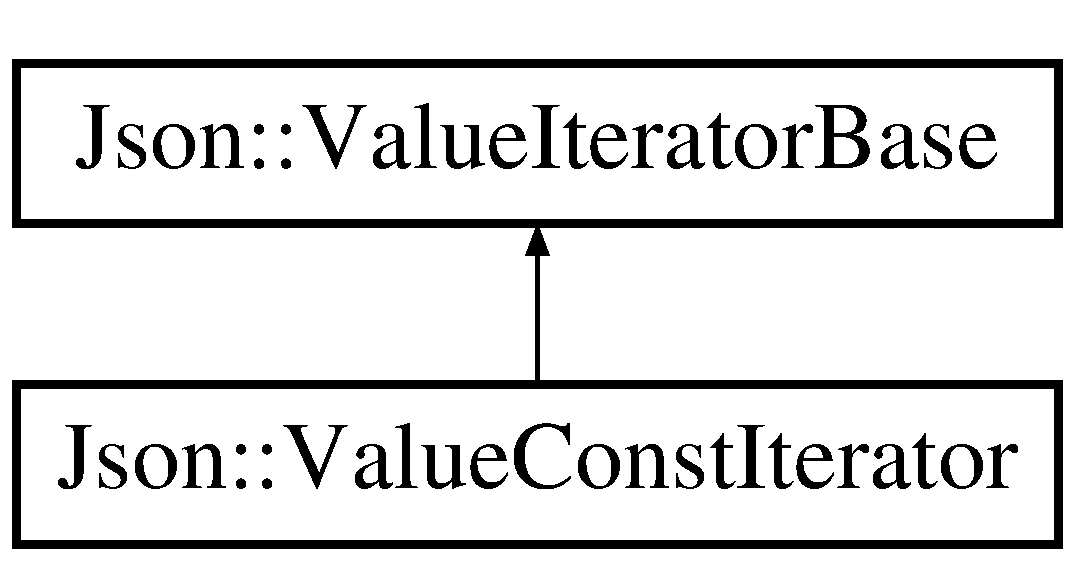
\includegraphics[height=2.000000cm]{class_json_1_1_value_const_iterator}
\end{center}
\end{figure}
\subsection*{Public Types}
\begin{DoxyCompactItemize}
\item 
typedef const \hyperlink{class_json_1_1_value}{Value} {\bfseries value\+\_\+type}\hypertarget{class_json_1_1_value_const_iterator_aa5f1707dcef4bfe73e23ddc14dbe760d}{}\label{class_json_1_1_value_const_iterator_aa5f1707dcef4bfe73e23ddc14dbe760d}

\item 
typedef const \hyperlink{class_json_1_1_value}{Value} \& {\bfseries reference}\hypertarget{class_json_1_1_value_const_iterator_aa9b05c6a37cd352ea1ee6e13b816f709}{}\label{class_json_1_1_value_const_iterator_aa9b05c6a37cd352ea1ee6e13b816f709}

\item 
typedef const \hyperlink{class_json_1_1_value}{Value} $\ast$ {\bfseries pointer}\hypertarget{class_json_1_1_value_const_iterator_a400136bd8bc09e9fddec0785fa2cff14}{}\label{class_json_1_1_value_const_iterator_a400136bd8bc09e9fddec0785fa2cff14}

\item 
typedef \hyperlink{class_json_1_1_value_const_iterator}{Value\+Const\+Iterator} {\bfseries Self\+Type}\hypertarget{class_json_1_1_value_const_iterator_a0c2e33e7eb5a80dd8709fb28ece83933}{}\label{class_json_1_1_value_const_iterator_a0c2e33e7eb5a80dd8709fb28ece83933}

\end{DoxyCompactItemize}
\subsection*{Public Member Functions}
\begin{DoxyCompactItemize}
\item 
{\bfseries Value\+Const\+Iterator} (\hyperlink{class_json_1_1_value_iterator}{Value\+Iterator} const \&other)\hypertarget{class_json_1_1_value_const_iterator_a7ef3df204a9ae83a0d8a3cd128e05c70}{}\label{class_json_1_1_value_const_iterator_a7ef3df204a9ae83a0d8a3cd128e05c70}

\item 
\hyperlink{class_json_1_1_value_iterator_base}{Self\+Type} \& {\bfseries operator=} (const \hyperlink{class_json_1_1_value_iterator_base}{Value\+Iterator\+Base} \&other)\hypertarget{class_json_1_1_value_const_iterator_ad1b1c11f8d7fb22d4d3c231915f2b15b}{}\label{class_json_1_1_value_const_iterator_ad1b1c11f8d7fb22d4d3c231915f2b15b}

\item 
\hyperlink{class_json_1_1_value_iterator_base}{Self\+Type} {\bfseries operator++} (int)\hypertarget{class_json_1_1_value_const_iterator_ab3f0c2edbfc8f7d60645f3d597d05e28}{}\label{class_json_1_1_value_const_iterator_ab3f0c2edbfc8f7d60645f3d597d05e28}

\item 
\hyperlink{class_json_1_1_value_iterator_base}{Self\+Type} {\bfseries operator-\/-\/} (int)\hypertarget{class_json_1_1_value_const_iterator_a94935961e9331c6f7b907b05ec8df75e}{}\label{class_json_1_1_value_const_iterator_a94935961e9331c6f7b907b05ec8df75e}

\item 
\hyperlink{class_json_1_1_value_iterator_base}{Self\+Type} \& {\bfseries operator-\/-\/} ()\hypertarget{class_json_1_1_value_const_iterator_a31415e44e44e56fb2bfda7e8bb784646}{}\label{class_json_1_1_value_const_iterator_a31415e44e44e56fb2bfda7e8bb784646}

\item 
\hyperlink{class_json_1_1_value_iterator_base}{Self\+Type} \& {\bfseries operator++} ()\hypertarget{class_json_1_1_value_const_iterator_a2cfe2f7a94a688186efdafb1b181c319}{}\label{class_json_1_1_value_const_iterator_a2cfe2f7a94a688186efdafb1b181c319}

\item 
\hyperlink{class_json_1_1_value}{reference} {\bfseries operator$\ast$} () const \hypertarget{class_json_1_1_value_const_iterator_aeb44153d71c61ac9397a84d5ecc244c5}{}\label{class_json_1_1_value_const_iterator_aeb44153d71c61ac9397a84d5ecc244c5}

\item 
\hyperlink{class_json_1_1_value}{pointer} {\bfseries operator-\/$>$} () const \hypertarget{class_json_1_1_value_const_iterator_ac493d31c8eede8af10b71415fe8e624b}{}\label{class_json_1_1_value_const_iterator_ac493d31c8eede8af10b71415fe8e624b}

\end{DoxyCompactItemize}
\subsection*{Friends}
\begin{DoxyCompactItemize}
\item 
class {\bfseries Value}\hypertarget{class_json_1_1_value_const_iterator_aeceedf6e1a7d48a588516ce2b1983d6f}{}\label{class_json_1_1_value_const_iterator_aeceedf6e1a7d48a588516ce2b1983d6f}

\end{DoxyCompactItemize}
\subsection*{Additional Inherited Members}


\subsection{Detailed Description}
const iterator for object and array value. 



The documentation for this class was generated from the following files\+:\begin{DoxyCompactItemize}
\item 
/home/andrea/\+Clion\+Projects/saas/lib/jsoncpp/inc/json.\+h\item 
/home/andrea/\+Clion\+Projects/saas/lib/jsoncpp/src/jsoncpp.\+cpp\end{DoxyCompactItemize}

\hypertarget{class_json_1_1_value_iterator}{}\section{Json\+:\+:Value\+Iterator Class Reference}
\label{class_json_1_1_value_iterator}\index{Json\+::\+Value\+Iterator@{Json\+::\+Value\+Iterator}}


Iterator for object and array value.  




{\ttfamily \#include $<$json.\+h$>$}

Inheritance diagram for Json\+:\+:Value\+Iterator\+:\begin{figure}[H]
\begin{center}
\leavevmode
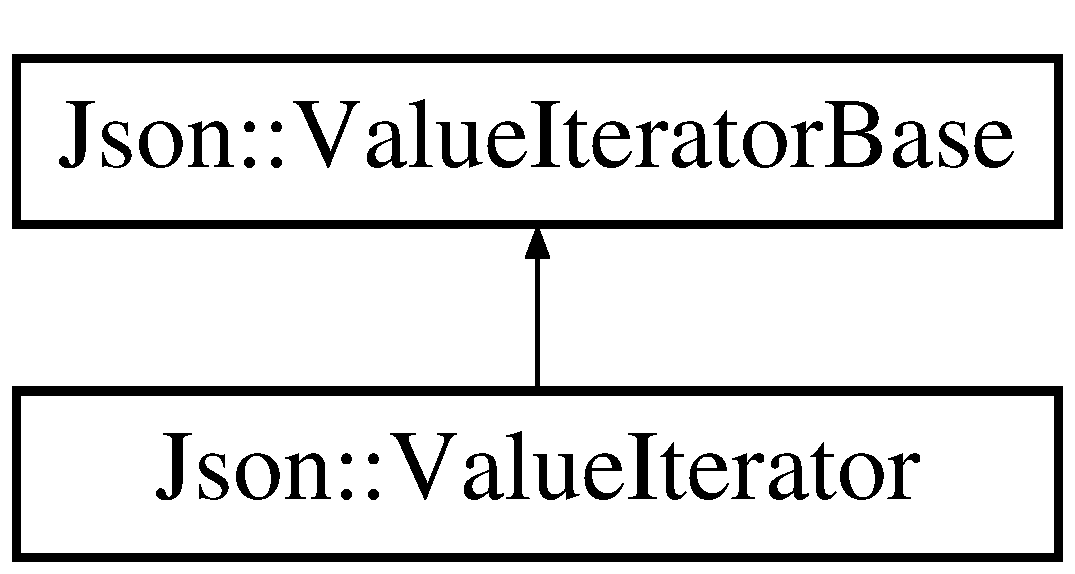
\includegraphics[height=2.000000cm]{class_json_1_1_value_iterator}
\end{center}
\end{figure}
\subsection*{Public Types}
\begin{DoxyCompactItemize}
\item 
typedef \hyperlink{class_json_1_1_value}{Value} {\bfseries value\+\_\+type}\hypertarget{class_json_1_1_value_iterator_a2c5ba7be611f05546530c8a88b2d2e37}{}\label{class_json_1_1_value_iterator_a2c5ba7be611f05546530c8a88b2d2e37}

\item 
typedef unsigned int {\bfseries size\+\_\+t}\hypertarget{class_json_1_1_value_iterator_a308b8932ffc83eaa9d12dadd5c11a7dd}{}\label{class_json_1_1_value_iterator_a308b8932ffc83eaa9d12dadd5c11a7dd}

\item 
typedef int {\bfseries difference\+\_\+type}\hypertarget{class_json_1_1_value_iterator_a2be1a9aa60bbfc8812e9dd1a7f1a8786}{}\label{class_json_1_1_value_iterator_a2be1a9aa60bbfc8812e9dd1a7f1a8786}

\item 
typedef \hyperlink{class_json_1_1_value}{Value} \& {\bfseries reference}\hypertarget{class_json_1_1_value_iterator_ae87929b4567aa00372cf602c43b57160}{}\label{class_json_1_1_value_iterator_ae87929b4567aa00372cf602c43b57160}

\item 
typedef \hyperlink{class_json_1_1_value}{Value} $\ast$ {\bfseries pointer}\hypertarget{class_json_1_1_value_iterator_acec45feb1ef1f3bf81240157d06d5432}{}\label{class_json_1_1_value_iterator_acec45feb1ef1f3bf81240157d06d5432}

\item 
typedef \hyperlink{class_json_1_1_value_iterator}{Value\+Iterator} {\bfseries Self\+Type}\hypertarget{class_json_1_1_value_iterator_a23357670fdad61792670d86f62db7e16}{}\label{class_json_1_1_value_iterator_a23357670fdad61792670d86f62db7e16}

\end{DoxyCompactItemize}
\subsection*{Public Member Functions}
\begin{DoxyCompactItemize}
\item 
{\bfseries Value\+Iterator} (const \hyperlink{class_json_1_1_value_const_iterator}{Value\+Const\+Iterator} \&other)\hypertarget{class_json_1_1_value_iterator_aa85aa208670891670392259efa0143bb}{}\label{class_json_1_1_value_iterator_aa85aa208670891670392259efa0143bb}

\item 
{\bfseries Value\+Iterator} (const \hyperlink{class_json_1_1_value_iterator}{Value\+Iterator} \&other)\hypertarget{class_json_1_1_value_iterator_a7d5e58a9a4a553968acdf3064b39d21c}{}\label{class_json_1_1_value_iterator_a7d5e58a9a4a553968acdf3064b39d21c}

\item 
\hyperlink{class_json_1_1_value_iterator_base}{Self\+Type} \& {\bfseries operator=} (const \hyperlink{class_json_1_1_value_iterator_base}{Self\+Type} \&other)\hypertarget{class_json_1_1_value_iterator_a8e23312b1db874f7e403fd7e76611bdc}{}\label{class_json_1_1_value_iterator_a8e23312b1db874f7e403fd7e76611bdc}

\item 
\hyperlink{class_json_1_1_value_iterator_base}{Self\+Type} {\bfseries operator++} (int)\hypertarget{class_json_1_1_value_iterator_abcf4ddd994a010742cd4a436d65acd08}{}\label{class_json_1_1_value_iterator_abcf4ddd994a010742cd4a436d65acd08}

\item 
\hyperlink{class_json_1_1_value_iterator_base}{Self\+Type} {\bfseries operator-\/-\/} (int)\hypertarget{class_json_1_1_value_iterator_a06d6a29d96caf6af324a53973159e12b}{}\label{class_json_1_1_value_iterator_a06d6a29d96caf6af324a53973159e12b}

\item 
\hyperlink{class_json_1_1_value_iterator_base}{Self\+Type} \& {\bfseries operator-\/-\/} ()\hypertarget{class_json_1_1_value_iterator_a811302a868518a0995a9def955df5720}{}\label{class_json_1_1_value_iterator_a811302a868518a0995a9def955df5720}

\item 
\hyperlink{class_json_1_1_value_iterator_base}{Self\+Type} \& {\bfseries operator++} ()\hypertarget{class_json_1_1_value_iterator_a92146c46f8249e2b2d12869e70cd4cee}{}\label{class_json_1_1_value_iterator_a92146c46f8249e2b2d12869e70cd4cee}

\item 
\hyperlink{class_json_1_1_value}{reference} {\bfseries operator$\ast$} () const \hypertarget{class_json_1_1_value_iterator_aaa5be3457eedf0526a03b8a3b4c7c0a0}{}\label{class_json_1_1_value_iterator_aaa5be3457eedf0526a03b8a3b4c7c0a0}

\item 
\hyperlink{class_json_1_1_value}{pointer} {\bfseries operator-\/$>$} () const \hypertarget{class_json_1_1_value_iterator_ad9882e4ce815cef6a504afa113544bfb}{}\label{class_json_1_1_value_iterator_ad9882e4ce815cef6a504afa113544bfb}

\end{DoxyCompactItemize}
\subsection*{Friends}
\begin{DoxyCompactItemize}
\item 
class {\bfseries Value}\hypertarget{class_json_1_1_value_iterator_aeceedf6e1a7d48a588516ce2b1983d6f}{}\label{class_json_1_1_value_iterator_aeceedf6e1a7d48a588516ce2b1983d6f}

\end{DoxyCompactItemize}
\subsection*{Additional Inherited Members}


\subsection{Detailed Description}
Iterator for object and array value. 

The documentation for this class was generated from the following files\+:\begin{DoxyCompactItemize}
\item 
/home/andrea/\+Clion\+Projects/saas/lib/jsoncpp/inc/json.\+h\item 
/home/andrea/\+Clion\+Projects/saas/lib/jsoncpp/src/jsoncpp.\+cpp\end{DoxyCompactItemize}

\hypertarget{class_json_1_1_value_iterator_base}{}\section{Json\+:\+:Value\+Iterator\+Base Class Reference}
\label{class_json_1_1_value_iterator_base}\index{Json\+::\+Value\+Iterator\+Base@{Json\+::\+Value\+Iterator\+Base}}


base class for \hyperlink{class_json_1_1_value}{Value} iterators.  




{\ttfamily \#include $<$json.\+h$>$}

Inheritance diagram for Json\+:\+:Value\+Iterator\+Base\+:\begin{figure}[H]
\begin{center}
\leavevmode
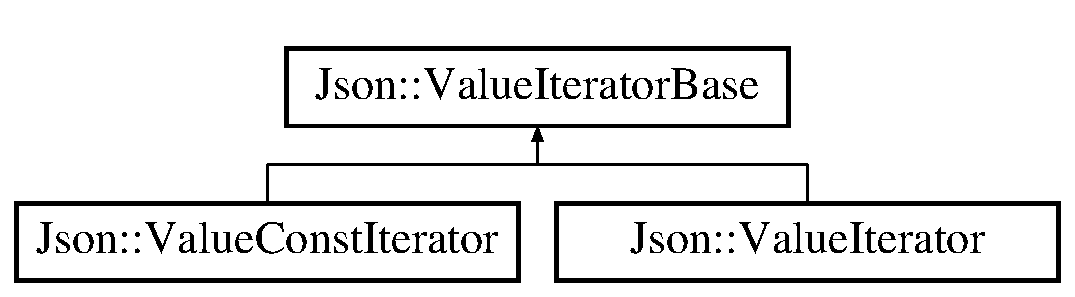
\includegraphics[height=2.000000cm]{class_json_1_1_value_iterator_base}
\end{center}
\end{figure}
\subsection*{Public Types}
\begin{DoxyCompactItemize}
\item 
\hypertarget{class_json_1_1_value_iterator_base_a02fd11a4fbdc0007da1e8bcf5e6b83c3}{}typedef std\+::bidirectional\+\_\+iterator\+\_\+tag {\bfseries iterator\+\_\+category}\label{class_json_1_1_value_iterator_base_a02fd11a4fbdc0007da1e8bcf5e6b83c3}

\item 
\hypertarget{class_json_1_1_value_iterator_base_a9d3a3c7ce5cdefe23cb486239cf07bb5}{}typedef unsigned int {\bfseries size\+\_\+t}\label{class_json_1_1_value_iterator_base_a9d3a3c7ce5cdefe23cb486239cf07bb5}

\item 
\hypertarget{class_json_1_1_value_iterator_base_a4e44bf8cbd17ec8d6e2c185904a15ebd}{}typedef int {\bfseries difference\+\_\+type}\label{class_json_1_1_value_iterator_base_a4e44bf8cbd17ec8d6e2c185904a15ebd}

\item 
\hypertarget{class_json_1_1_value_iterator_base_a9d2a940d03ea06d20d972f41a89149ee}{}typedef \hyperlink{class_json_1_1_value_iterator_base}{Value\+Iterator\+Base} {\bfseries Self\+Type}\label{class_json_1_1_value_iterator_base_a9d2a940d03ea06d20d972f41a89149ee}

\end{DoxyCompactItemize}
\subsection*{Public Member Functions}
\begin{DoxyCompactItemize}
\item 
\hypertarget{class_json_1_1_value_iterator_base_afc656672ac28502f640ade32c38c1b56}{}bool {\bfseries operator==} (const \hyperlink{class_json_1_1_value_iterator_base}{Self\+Type} \&other) const \label{class_json_1_1_value_iterator_base_afc656672ac28502f640ade32c38c1b56}

\item 
\hypertarget{class_json_1_1_value_iterator_base_a18c2dd42e0bb989ace141bfe9de52792}{}bool {\bfseries operator!=} (const \hyperlink{class_json_1_1_value_iterator_base}{Self\+Type} \&other) const \label{class_json_1_1_value_iterator_base_a18c2dd42e0bb989ace141bfe9de52792}

\item 
\hypertarget{class_json_1_1_value_iterator_base_ab786787fcad68ca5e8745aaf520fa17f}{}difference\+\_\+type {\bfseries operator-\/} (const \hyperlink{class_json_1_1_value_iterator_base}{Self\+Type} \&other) const \label{class_json_1_1_value_iterator_base_ab786787fcad68ca5e8745aaf520fa17f}

\item 
\hyperlink{class_json_1_1_value}{Value} \hyperlink{class_json_1_1_value_iterator_base_aa2ff5e79fc96acd4c3cd288e92614fc7}{key} () const 
\item 
\hypertarget{class_json_1_1_value_iterator_base_aa90591f5f7f8d2f06cc4605816b53738}{}U\+Int \hyperlink{class_json_1_1_value_iterator_base_aa90591f5f7f8d2f06cc4605816b53738}{index} () const \label{class_json_1_1_value_iterator_base_aa90591f5f7f8d2f06cc4605816b53738}

\begin{DoxyCompactList}\small\item\em Return the index of the referenced \hyperlink{class_json_1_1_value}{Value}, or -\/1 if it is not an array\+Value. \end{DoxyCompactList}\item 
std\+::string \hyperlink{class_json_1_1_value_iterator_base_a46a67081a5ef8d83f25ec15035403ce0}{name} () const 
\item 
char const $\ast$ \hyperlink{class_json_1_1_value_iterator_base_ac3aa3870761342e47c6486d81f643c6c}{member\+Name} () const 
\item 
char const $\ast$ \hyperlink{class_json_1_1_value_iterator_base_a543d4e73e3d2d121bc287b24231386c3}{member\+Name} (char const $\ast$$\ast$end) const 
\item 
\hypertarget{class_json_1_1_value_iterator_base_a640e990e5f03a96fd650122a2906f59d}{}{\bfseries Value\+Iterator\+Base} (const Value\+::\+Object\+Values\+::iterator \&current)\label{class_json_1_1_value_iterator_base_a640e990e5f03a96fd650122a2906f59d}

\end{DoxyCompactItemize}
\subsection*{Protected Member Functions}
\begin{DoxyCompactItemize}
\item 
\hypertarget{class_json_1_1_value_iterator_base_a40a20c65abc423a26e3aae68d9a0525c}{}\hyperlink{class_json_1_1_value}{Value} \& {\bfseries deref} () const \label{class_json_1_1_value_iterator_base_a40a20c65abc423a26e3aae68d9a0525c}

\item 
\hypertarget{class_json_1_1_value_iterator_base_afe58f9534e1fd2033419fd9fe244551e}{}void {\bfseries increment} ()\label{class_json_1_1_value_iterator_base_afe58f9534e1fd2033419fd9fe244551e}

\item 
\hypertarget{class_json_1_1_value_iterator_base_affc8cf5ff54a9f432cc693362c153fa6}{}void {\bfseries decrement} ()\label{class_json_1_1_value_iterator_base_affc8cf5ff54a9f432cc693362c153fa6}

\item 
\hypertarget{class_json_1_1_value_iterator_base_ad6c553b249e89e3dc9933e100ccbe064}{}difference\+\_\+type {\bfseries compute\+Distance} (const \hyperlink{class_json_1_1_value_iterator_base}{Self\+Type} \&other) const \label{class_json_1_1_value_iterator_base_ad6c553b249e89e3dc9933e100ccbe064}

\item 
\hypertarget{class_json_1_1_value_iterator_base_a21820d6ee564e541bd118b21e4741962}{}bool {\bfseries is\+Equal} (const \hyperlink{class_json_1_1_value_iterator_base}{Self\+Type} \&other) const \label{class_json_1_1_value_iterator_base_a21820d6ee564e541bd118b21e4741962}

\item 
\hypertarget{class_json_1_1_value_iterator_base_a496e6aba44808433ec5858c178be5719}{}void {\bfseries copy} (const \hyperlink{class_json_1_1_value_iterator_base}{Self\+Type} \&other)\label{class_json_1_1_value_iterator_base_a496e6aba44808433ec5858c178be5719}

\end{DoxyCompactItemize}


\subsection{Detailed Description}
base class for \hyperlink{class_json_1_1_value}{Value} iterators. 



\subsection{Member Function Documentation}
\hypertarget{class_json_1_1_value_iterator_base_aa2ff5e79fc96acd4c3cd288e92614fc7}{}\index{Json\+::\+Value\+Iterator\+Base@{Json\+::\+Value\+Iterator\+Base}!key@{key}}
\index{key@{key}!Json\+::\+Value\+Iterator\+Base@{Json\+::\+Value\+Iterator\+Base}}
\subsubsection[{key}]{\setlength{\rightskip}{0pt plus 5cm}{\bf Value} Json\+::\+Value\+Iterator\+Base\+::key (
\begin{DoxyParamCaption}
{}
\end{DoxyParamCaption}
) const}\label{class_json_1_1_value_iterator_base_aa2ff5e79fc96acd4c3cd288e92614fc7}
Return either the index or the member name of the referenced value as a \hyperlink{class_json_1_1_value}{Value}. \hypertarget{class_json_1_1_value_iterator_base_ac3aa3870761342e47c6486d81f643c6c}{}\index{Json\+::\+Value\+Iterator\+Base@{Json\+::\+Value\+Iterator\+Base}!member\+Name@{member\+Name}}
\index{member\+Name@{member\+Name}!Json\+::\+Value\+Iterator\+Base@{Json\+::\+Value\+Iterator\+Base}}
\subsubsection[{member\+Name}]{\setlength{\rightskip}{0pt plus 5cm}char const $\ast$ Json\+::\+Value\+Iterator\+Base\+::member\+Name (
\begin{DoxyParamCaption}
{}
\end{DoxyParamCaption}
) const}\label{class_json_1_1_value_iterator_base_ac3aa3870761342e47c6486d81f643c6c}
Return the member name of the referenced \hyperlink{class_json_1_1_value}{Value}. \char`\"{}\char`\"{} if it is not an object\+Value. \begin{DoxyRefDesc}{Deprecated}
\item[\hyperlink{deprecated__deprecated000004}{Deprecated}]This cannot be used for U\+T\+F-\/8 strings, since there can be embedded nulls. \end{DoxyRefDesc}
\hypertarget{class_json_1_1_value_iterator_base_a543d4e73e3d2d121bc287b24231386c3}{}\index{Json\+::\+Value\+Iterator\+Base@{Json\+::\+Value\+Iterator\+Base}!member\+Name@{member\+Name}}
\index{member\+Name@{member\+Name}!Json\+::\+Value\+Iterator\+Base@{Json\+::\+Value\+Iterator\+Base}}
\subsubsection[{member\+Name}]{\setlength{\rightskip}{0pt plus 5cm}char const $\ast$ Json\+::\+Value\+Iterator\+Base\+::member\+Name (
\begin{DoxyParamCaption}
\item[{char const $\ast$$\ast$}]{end}
\end{DoxyParamCaption}
) const}\label{class_json_1_1_value_iterator_base_a543d4e73e3d2d121bc287b24231386c3}
Return the member name of the referenced \hyperlink{class_json_1_1_value}{Value}, or N\+U\+L\+L if it is not an object\+Value. \begin{DoxyNote}{Note}
Better version than \hyperlink{class_json_1_1_value_iterator_base_ac3aa3870761342e47c6486d81f643c6c}{member\+Name()}. Allows embedded nulls. 
\end{DoxyNote}
\hypertarget{class_json_1_1_value_iterator_base_a46a67081a5ef8d83f25ec15035403ce0}{}\index{Json\+::\+Value\+Iterator\+Base@{Json\+::\+Value\+Iterator\+Base}!name@{name}}
\index{name@{name}!Json\+::\+Value\+Iterator\+Base@{Json\+::\+Value\+Iterator\+Base}}
\subsubsection[{name}]{\setlength{\rightskip}{0pt plus 5cm}std\+::string Json\+::\+Value\+Iterator\+Base\+::name (
\begin{DoxyParamCaption}
{}
\end{DoxyParamCaption}
) const}\label{class_json_1_1_value_iterator_base_a46a67081a5ef8d83f25ec15035403ce0}
Return the member name of the referenced \hyperlink{class_json_1_1_value}{Value}, or \char`\"{}\char`\"{} if it is not an object\+Value. \begin{DoxyNote}{Note}
Avoid {\ttfamily c\+\_\+str()} on result, as embedded zeroes are possible. 
\end{DoxyNote}


The documentation for this class was generated from the following files\+:\begin{DoxyCompactItemize}
\item 
/home/frank/dev/cpe402/saas/lib/jsoncpp/inc/json.\+h\item 
/home/frank/dev/cpe402/saas/lib/jsoncpp/src/jsoncpp.\+cpp\end{DoxyCompactItemize}

\hypertarget{class_example_1_1_vector}{}\section{Example.\+Vector Class Reference}
\label{class_example_1_1_vector}\index{Example.\+Vector@{Example.\+Vector}}


 


\subsection*{Public Member Functions}
\begin{DoxyCompactItemize}
\item 
\hypertarget{class_example_1_1_vector_ac17d93480759cbcdcafaefb1e9e2181f}{}{\bfseries Vector} (float x, float y, float z)\label{class_example_1_1_vector_ac17d93480759cbcdcafaefb1e9e2181f}

\end{DoxyCompactItemize}
\subsection*{Static Public Member Functions}
\begin{DoxyCompactItemize}
\item 
static \hyperlink{class_example_1_1_vector}{Vector} \hyperlink{class_example_1_1_vector_a818efcb4e8291291770ef378c1f25e9e}{Deserialize} (Stream stream)
\begin{DoxyCompactList}\small\item\em Helper\+: create a new instance to deserializing into\end{DoxyCompactList}\item 
static \hyperlink{class_example_1_1_vector}{Vector} \hyperlink{class_example_1_1_vector_ac0d43068ece1c2630c4251dff5e8ada0}{Deserialize\+Length\+Delimited} (Stream stream)
\begin{DoxyCompactList}\small\item\em Helper\+: create a new instance to deserializing into\end{DoxyCompactList}\item 
static \hyperlink{class_example_1_1_vector}{Vector} \hyperlink{class_example_1_1_vector_abe963061d88c30a7242d5bb92828d18f}{Deserialize\+Length} (Stream stream, int length)
\begin{DoxyCompactList}\small\item\em Helper\+: create a new instance to deserializing into\end{DoxyCompactList}\item 
static \hyperlink{class_example_1_1_vector}{Vector} \hyperlink{class_example_1_1_vector_a9f29e4e1efdfb2e0841623ff2311cce5}{Deserialize} (byte\mbox{[}$\,$\mbox{]} buffer)
\begin{DoxyCompactList}\small\item\em Helper\+: put the buffer into a Memory\+Stream and create a new instance to deserializing into\end{DoxyCompactList}\item 
static \hyperlink{class_example_1_1_vector}{Example.\+Vector} \hyperlink{class_example_1_1_vector_a2bedbd5f974dd3d18fc86300b673f55d}{Deserialize} (byte\mbox{[}$\,$\mbox{]} buffer, \hyperlink{class_example_1_1_vector}{Example.\+Vector} instance)
\begin{DoxyCompactList}\small\item\em Helper\+: put the buffer into a Memory\+Stream before deserializing\end{DoxyCompactList}\item 
static \hyperlink{class_example_1_1_vector}{Example.\+Vector} \hyperlink{class_example_1_1_vector_a1eaf2f0f8c1289888fa799ad8c16fa21}{Deserialize} (Stream stream, \hyperlink{class_example_1_1_vector}{Example.\+Vector} instance)
\begin{DoxyCompactList}\small\item\em Takes the remaining content of the stream and deserialze it into the instance.\end{DoxyCompactList}\item 
static \hyperlink{class_example_1_1_vector}{Example.\+Vector} \hyperlink{class_example_1_1_vector_a3092148f5634ca0cc425bcb6f83c5533}{Deserialize\+Length\+Delimited} (Stream stream, \hyperlink{class_example_1_1_vector}{Example.\+Vector} instance)
\begin{DoxyCompactList}\small\item\em Read the Var\+Int length prefix and the given number of bytes from the stream and deserialze it into the instance.\end{DoxyCompactList}\item 
static \hyperlink{class_example_1_1_vector}{Example.\+Vector} \hyperlink{class_example_1_1_vector_aa5e9f156e0489ef1c5bc9578dfd545a1}{Deserialize\+Length} (Stream stream, int length, \hyperlink{class_example_1_1_vector}{Example.\+Vector} instance)
\begin{DoxyCompactList}\small\item\em Read the given number of bytes from the stream and deserialze it into the instance.\end{DoxyCompactList}\item 
static void \hyperlink{class_example_1_1_vector_af60b9bcba3c2dddfc4ef780c5d2786c6}{Serialize} (Stream stream, \hyperlink{class_example_1_1_vector}{Vector} instance)
\begin{DoxyCompactList}\small\item\em Serialize the instance into the stream\end{DoxyCompactList}\item 
static byte\mbox{[}$\,$\mbox{]} \hyperlink{class_example_1_1_vector_aae89c55b304738980925ebbcfdbfa946}{Serialize\+To\+Bytes} (\hyperlink{class_example_1_1_vector}{Vector} instance)
\begin{DoxyCompactList}\small\item\em Helper\+: Serialize into a Memory\+Stream and return its byte array\end{DoxyCompactList}\item 
static void \hyperlink{class_example_1_1_vector_ad5dad3812b90c5fe6669407f8588fbf5}{Serialize\+Length\+Delimited} (Stream stream, \hyperlink{class_example_1_1_vector}{Vector} instance)
\begin{DoxyCompactList}\small\item\em Helper\+: Serialize with a varint length prefix\end{DoxyCompactList}\item 
static \hyperlink{class_example_1_1_vector}{Vector} \hyperlink{class_example_1_1_vector_a818efcb4e8291291770ef378c1f25e9e}{Deserialize} (Stream stream)
\begin{DoxyCompactList}\small\item\em Helper\+: create a new instance to deserializing into\end{DoxyCompactList}\item 
static \hyperlink{class_example_1_1_vector}{Vector} \hyperlink{class_example_1_1_vector_ac0d43068ece1c2630c4251dff5e8ada0}{Deserialize\+Length\+Delimited} (Stream stream)
\begin{DoxyCompactList}\small\item\em Helper\+: create a new instance to deserializing into\end{DoxyCompactList}\item 
static \hyperlink{class_example_1_1_vector}{Vector} \hyperlink{class_example_1_1_vector_abe963061d88c30a7242d5bb92828d18f}{Deserialize\+Length} (Stream stream, int length)
\begin{DoxyCompactList}\small\item\em Helper\+: create a new instance to deserializing into\end{DoxyCompactList}\item 
static \hyperlink{class_example_1_1_vector}{Vector} \hyperlink{class_example_1_1_vector_a9f29e4e1efdfb2e0841623ff2311cce5}{Deserialize} (byte\mbox{[}$\,$\mbox{]} buffer)
\begin{DoxyCompactList}\small\item\em Helper\+: put the buffer into a Memory\+Stream and create a new instance to deserializing into\end{DoxyCompactList}\item 
static \hyperlink{class_example_1_1_vector}{Example.\+Vector} \hyperlink{class_example_1_1_vector_a2bedbd5f974dd3d18fc86300b673f55d}{Deserialize} (byte\mbox{[}$\,$\mbox{]} buffer, \hyperlink{class_example_1_1_vector}{Example.\+Vector} instance)
\begin{DoxyCompactList}\small\item\em Helper\+: put the buffer into a Memory\+Stream before deserializing\end{DoxyCompactList}\item 
static \hyperlink{class_example_1_1_vector}{Example.\+Vector} \hyperlink{class_example_1_1_vector_a1eaf2f0f8c1289888fa799ad8c16fa21}{Deserialize} (Stream stream, \hyperlink{class_example_1_1_vector}{Example.\+Vector} instance)
\begin{DoxyCompactList}\small\item\em Takes the remaining content of the stream and deserialze it into the instance.\end{DoxyCompactList}\item 
static \hyperlink{class_example_1_1_vector}{Example.\+Vector} \hyperlink{class_example_1_1_vector_a3092148f5634ca0cc425bcb6f83c5533}{Deserialize\+Length\+Delimited} (Stream stream, \hyperlink{class_example_1_1_vector}{Example.\+Vector} instance)
\begin{DoxyCompactList}\small\item\em Read the Var\+Int length prefix and the given number of bytes from the stream and deserialze it into the instance.\end{DoxyCompactList}\item 
static \hyperlink{class_example_1_1_vector}{Example.\+Vector} \hyperlink{class_example_1_1_vector_aa5e9f156e0489ef1c5bc9578dfd545a1}{Deserialize\+Length} (Stream stream, int length, \hyperlink{class_example_1_1_vector}{Example.\+Vector} instance)
\begin{DoxyCompactList}\small\item\em Read the given number of bytes from the stream and deserialze it into the instance.\end{DoxyCompactList}\item 
static void \hyperlink{class_example_1_1_vector_af60b9bcba3c2dddfc4ef780c5d2786c6}{Serialize} (Stream stream, \hyperlink{class_example_1_1_vector}{Vector} instance)
\begin{DoxyCompactList}\small\item\em Serialize the instance into the stream\end{DoxyCompactList}\item 
static byte\mbox{[}$\,$\mbox{]} \hyperlink{class_example_1_1_vector_aae89c55b304738980925ebbcfdbfa946}{Serialize\+To\+Bytes} (\hyperlink{class_example_1_1_vector}{Vector} instance)
\begin{DoxyCompactList}\small\item\em Helper\+: Serialize into a Memory\+Stream and return its byte array\end{DoxyCompactList}\item 
static void \hyperlink{class_example_1_1_vector_ad5dad3812b90c5fe6669407f8588fbf5}{Serialize\+Length\+Delimited} (Stream stream, \hyperlink{class_example_1_1_vector}{Vector} instance)
\begin{DoxyCompactList}\small\item\em Helper\+: Serialize with a varint length prefix\end{DoxyCompactList}\end{DoxyCompactItemize}
\subsection*{Properties}
\begin{DoxyCompactItemize}
\item 
\hypertarget{class_example_1_1_vector_a91797e953010f556b85a7173e644d957}{}float {\bfseries N}\hspace{0.3cm}{\ttfamily  \mbox{[}get, set\mbox{]}}\label{class_example_1_1_vector_a91797e953010f556b85a7173e644d957}

\item 
\hypertarget{class_example_1_1_vector_aa0495aefcfa8d8ec5bdd147a91de8571}{}float {\bfseries E}\hspace{0.3cm}{\ttfamily  \mbox{[}get, set\mbox{]}}\label{class_example_1_1_vector_aa0495aefcfa8d8ec5bdd147a91de8571}

\item 
\hypertarget{class_example_1_1_vector_a66424f9c546909c67d9697d7546d525f}{}float {\bfseries D}\hspace{0.3cm}{\ttfamily  \mbox{[}get, set\mbox{]}}\label{class_example_1_1_vector_a66424f9c546909c67d9697d7546d525f}

\item 
\hypertarget{class_example_1_1_vector_a93704a1572edef07ab0a97d2c49f31ed}{}float {\bfseries X}\hspace{0.3cm}{\ttfamily  \mbox{[}get, set\mbox{]}}\label{class_example_1_1_vector_a93704a1572edef07ab0a97d2c49f31ed}

\item 
\hypertarget{class_example_1_1_vector_ab46c21e0af1a734923c4124b3d62353f}{}float {\bfseries Y}\hspace{0.3cm}{\ttfamily  \mbox{[}get, set\mbox{]}}\label{class_example_1_1_vector_ab46c21e0af1a734923c4124b3d62353f}

\item 
\hypertarget{class_example_1_1_vector_a1d9fa339dc2741d619f11cfb1d7f99d8}{}float {\bfseries Z}\hspace{0.3cm}{\ttfamily  \mbox{[}get, set\mbox{]}}\label{class_example_1_1_vector_a1d9fa339dc2741d619f11cfb1d7f99d8}

\end{DoxyCompactItemize}


\subsection{Detailed Description}


$\ast$

$\ast$ Coordinate System

$\ast$ X\+: Positive is Right along the C\+D\+T\+I, Negative is Left.

$\ast$ Y\+: Positive is Up along the C\+D\+T\+I, Negative is Down.

$\ast$ Z\+: Positive is above the ship in C\+D\+T\+I, Negative is below.

\subsection{Member Function Documentation}
\hypertarget{class_example_1_1_vector_a818efcb4e8291291770ef378c1f25e9e}{}\index{Example\+::\+Vector@{Example\+::\+Vector}!Deserialize@{Deserialize}}
\index{Deserialize@{Deserialize}!Example\+::\+Vector@{Example\+::\+Vector}}
\subsubsection[{Deserialize}]{\setlength{\rightskip}{0pt plus 5cm}static {\bf Vector} Example.\+Vector.\+Deserialize (
\begin{DoxyParamCaption}
\item[{Stream}]{stream}
\end{DoxyParamCaption}
)\hspace{0.3cm}{\ttfamily [inline]}, {\ttfamily [static]}}\label{class_example_1_1_vector_a818efcb4e8291291770ef378c1f25e9e}


Helper\+: create a new instance to deserializing into

\hypertarget{class_example_1_1_vector_a818efcb4e8291291770ef378c1f25e9e}{}\index{Example\+::\+Vector@{Example\+::\+Vector}!Deserialize@{Deserialize}}
\index{Deserialize@{Deserialize}!Example\+::\+Vector@{Example\+::\+Vector}}
\subsubsection[{Deserialize}]{\setlength{\rightskip}{0pt plus 5cm}static {\bf Vector} Example.\+Vector.\+Deserialize (
\begin{DoxyParamCaption}
\item[{Stream}]{stream}
\end{DoxyParamCaption}
)\hspace{0.3cm}{\ttfamily [inline]}, {\ttfamily [static]}}\label{class_example_1_1_vector_a818efcb4e8291291770ef378c1f25e9e}


Helper\+: create a new instance to deserializing into

\hypertarget{class_example_1_1_vector_a9f29e4e1efdfb2e0841623ff2311cce5}{}\index{Example\+::\+Vector@{Example\+::\+Vector}!Deserialize@{Deserialize}}
\index{Deserialize@{Deserialize}!Example\+::\+Vector@{Example\+::\+Vector}}
\subsubsection[{Deserialize}]{\setlength{\rightskip}{0pt plus 5cm}static {\bf Vector} Example.\+Vector.\+Deserialize (
\begin{DoxyParamCaption}
\item[{byte\mbox{[}$\,$\mbox{]}}]{buffer}
\end{DoxyParamCaption}
)\hspace{0.3cm}{\ttfamily [inline]}, {\ttfamily [static]}}\label{class_example_1_1_vector_a9f29e4e1efdfb2e0841623ff2311cce5}


Helper\+: put the buffer into a Memory\+Stream and create a new instance to deserializing into

\hypertarget{class_example_1_1_vector_a9f29e4e1efdfb2e0841623ff2311cce5}{}\index{Example\+::\+Vector@{Example\+::\+Vector}!Deserialize@{Deserialize}}
\index{Deserialize@{Deserialize}!Example\+::\+Vector@{Example\+::\+Vector}}
\subsubsection[{Deserialize}]{\setlength{\rightskip}{0pt plus 5cm}static {\bf Vector} Example.\+Vector.\+Deserialize (
\begin{DoxyParamCaption}
\item[{byte\mbox{[}$\,$\mbox{]}}]{buffer}
\end{DoxyParamCaption}
)\hspace{0.3cm}{\ttfamily [inline]}, {\ttfamily [static]}}\label{class_example_1_1_vector_a9f29e4e1efdfb2e0841623ff2311cce5}


Helper\+: put the buffer into a Memory\+Stream and create a new instance to deserializing into

\hypertarget{class_example_1_1_vector_a2bedbd5f974dd3d18fc86300b673f55d}{}\index{Example\+::\+Vector@{Example\+::\+Vector}!Deserialize@{Deserialize}}
\index{Deserialize@{Deserialize}!Example\+::\+Vector@{Example\+::\+Vector}}
\subsubsection[{Deserialize}]{\setlength{\rightskip}{0pt plus 5cm}static {\bf Example.\+Vector} Example.\+Vector.\+Deserialize (
\begin{DoxyParamCaption}
\item[{byte\mbox{[}$\,$\mbox{]}}]{buffer, }
\item[{{\bf Example.\+Vector}}]{instance}
\end{DoxyParamCaption}
)\hspace{0.3cm}{\ttfamily [inline]}, {\ttfamily [static]}}\label{class_example_1_1_vector_a2bedbd5f974dd3d18fc86300b673f55d}


Helper\+: put the buffer into a Memory\+Stream before deserializing

\hypertarget{class_example_1_1_vector_a2bedbd5f974dd3d18fc86300b673f55d}{}\index{Example\+::\+Vector@{Example\+::\+Vector}!Deserialize@{Deserialize}}
\index{Deserialize@{Deserialize}!Example\+::\+Vector@{Example\+::\+Vector}}
\subsubsection[{Deserialize}]{\setlength{\rightskip}{0pt plus 5cm}static {\bf Example.\+Vector} Example.\+Vector.\+Deserialize (
\begin{DoxyParamCaption}
\item[{byte\mbox{[}$\,$\mbox{]}}]{buffer, }
\item[{{\bf Example.\+Vector}}]{instance}
\end{DoxyParamCaption}
)\hspace{0.3cm}{\ttfamily [inline]}, {\ttfamily [static]}}\label{class_example_1_1_vector_a2bedbd5f974dd3d18fc86300b673f55d}


Helper\+: put the buffer into a Memory\+Stream before deserializing

\hypertarget{class_example_1_1_vector_a1eaf2f0f8c1289888fa799ad8c16fa21}{}\index{Example\+::\+Vector@{Example\+::\+Vector}!Deserialize@{Deserialize}}
\index{Deserialize@{Deserialize}!Example\+::\+Vector@{Example\+::\+Vector}}
\subsubsection[{Deserialize}]{\setlength{\rightskip}{0pt plus 5cm}static {\bf Example.\+Vector} Example.\+Vector.\+Deserialize (
\begin{DoxyParamCaption}
\item[{Stream}]{stream, }
\item[{{\bf Example.\+Vector}}]{instance}
\end{DoxyParamCaption}
)\hspace{0.3cm}{\ttfamily [inline]}, {\ttfamily [static]}}\label{class_example_1_1_vector_a1eaf2f0f8c1289888fa799ad8c16fa21}


Takes the remaining content of the stream and deserialze it into the instance.

\hypertarget{class_example_1_1_vector_a1eaf2f0f8c1289888fa799ad8c16fa21}{}\index{Example\+::\+Vector@{Example\+::\+Vector}!Deserialize@{Deserialize}}
\index{Deserialize@{Deserialize}!Example\+::\+Vector@{Example\+::\+Vector}}
\subsubsection[{Deserialize}]{\setlength{\rightskip}{0pt plus 5cm}static {\bf Example.\+Vector} Example.\+Vector.\+Deserialize (
\begin{DoxyParamCaption}
\item[{Stream}]{stream, }
\item[{{\bf Example.\+Vector}}]{instance}
\end{DoxyParamCaption}
)\hspace{0.3cm}{\ttfamily [inline]}, {\ttfamily [static]}}\label{class_example_1_1_vector_a1eaf2f0f8c1289888fa799ad8c16fa21}


Takes the remaining content of the stream and deserialze it into the instance.

\hypertarget{class_example_1_1_vector_abe963061d88c30a7242d5bb92828d18f}{}\index{Example\+::\+Vector@{Example\+::\+Vector}!Deserialize\+Length@{Deserialize\+Length}}
\index{Deserialize\+Length@{Deserialize\+Length}!Example\+::\+Vector@{Example\+::\+Vector}}
\subsubsection[{Deserialize\+Length}]{\setlength{\rightskip}{0pt plus 5cm}static {\bf Vector} Example.\+Vector.\+Deserialize\+Length (
\begin{DoxyParamCaption}
\item[{Stream}]{stream, }
\item[{int}]{length}
\end{DoxyParamCaption}
)\hspace{0.3cm}{\ttfamily [inline]}, {\ttfamily [static]}}\label{class_example_1_1_vector_abe963061d88c30a7242d5bb92828d18f}


Helper\+: create a new instance to deserializing into

\hypertarget{class_example_1_1_vector_abe963061d88c30a7242d5bb92828d18f}{}\index{Example\+::\+Vector@{Example\+::\+Vector}!Deserialize\+Length@{Deserialize\+Length}}
\index{Deserialize\+Length@{Deserialize\+Length}!Example\+::\+Vector@{Example\+::\+Vector}}
\subsubsection[{Deserialize\+Length}]{\setlength{\rightskip}{0pt plus 5cm}static {\bf Vector} Example.\+Vector.\+Deserialize\+Length (
\begin{DoxyParamCaption}
\item[{Stream}]{stream, }
\item[{int}]{length}
\end{DoxyParamCaption}
)\hspace{0.3cm}{\ttfamily [inline]}, {\ttfamily [static]}}\label{class_example_1_1_vector_abe963061d88c30a7242d5bb92828d18f}


Helper\+: create a new instance to deserializing into

\hypertarget{class_example_1_1_vector_aa5e9f156e0489ef1c5bc9578dfd545a1}{}\index{Example\+::\+Vector@{Example\+::\+Vector}!Deserialize\+Length@{Deserialize\+Length}}
\index{Deserialize\+Length@{Deserialize\+Length}!Example\+::\+Vector@{Example\+::\+Vector}}
\subsubsection[{Deserialize\+Length}]{\setlength{\rightskip}{0pt plus 5cm}static {\bf Example.\+Vector} Example.\+Vector.\+Deserialize\+Length (
\begin{DoxyParamCaption}
\item[{Stream}]{stream, }
\item[{int}]{length, }
\item[{{\bf Example.\+Vector}}]{instance}
\end{DoxyParamCaption}
)\hspace{0.3cm}{\ttfamily [inline]}, {\ttfamily [static]}}\label{class_example_1_1_vector_aa5e9f156e0489ef1c5bc9578dfd545a1}


Read the given number of bytes from the stream and deserialze it into the instance.

\hypertarget{class_example_1_1_vector_aa5e9f156e0489ef1c5bc9578dfd545a1}{}\index{Example\+::\+Vector@{Example\+::\+Vector}!Deserialize\+Length@{Deserialize\+Length}}
\index{Deserialize\+Length@{Deserialize\+Length}!Example\+::\+Vector@{Example\+::\+Vector}}
\subsubsection[{Deserialize\+Length}]{\setlength{\rightskip}{0pt plus 5cm}static {\bf Example.\+Vector} Example.\+Vector.\+Deserialize\+Length (
\begin{DoxyParamCaption}
\item[{Stream}]{stream, }
\item[{int}]{length, }
\item[{{\bf Example.\+Vector}}]{instance}
\end{DoxyParamCaption}
)\hspace{0.3cm}{\ttfamily [inline]}, {\ttfamily [static]}}\label{class_example_1_1_vector_aa5e9f156e0489ef1c5bc9578dfd545a1}


Read the given number of bytes from the stream and deserialze it into the instance.

\hypertarget{class_example_1_1_vector_ac0d43068ece1c2630c4251dff5e8ada0}{}\index{Example\+::\+Vector@{Example\+::\+Vector}!Deserialize\+Length\+Delimited@{Deserialize\+Length\+Delimited}}
\index{Deserialize\+Length\+Delimited@{Deserialize\+Length\+Delimited}!Example\+::\+Vector@{Example\+::\+Vector}}
\subsubsection[{Deserialize\+Length\+Delimited}]{\setlength{\rightskip}{0pt plus 5cm}static {\bf Vector} Example.\+Vector.\+Deserialize\+Length\+Delimited (
\begin{DoxyParamCaption}
\item[{Stream}]{stream}
\end{DoxyParamCaption}
)\hspace{0.3cm}{\ttfamily [inline]}, {\ttfamily [static]}}\label{class_example_1_1_vector_ac0d43068ece1c2630c4251dff5e8ada0}


Helper\+: create a new instance to deserializing into

\hypertarget{class_example_1_1_vector_ac0d43068ece1c2630c4251dff5e8ada0}{}\index{Example\+::\+Vector@{Example\+::\+Vector}!Deserialize\+Length\+Delimited@{Deserialize\+Length\+Delimited}}
\index{Deserialize\+Length\+Delimited@{Deserialize\+Length\+Delimited}!Example\+::\+Vector@{Example\+::\+Vector}}
\subsubsection[{Deserialize\+Length\+Delimited}]{\setlength{\rightskip}{0pt plus 5cm}static {\bf Vector} Example.\+Vector.\+Deserialize\+Length\+Delimited (
\begin{DoxyParamCaption}
\item[{Stream}]{stream}
\end{DoxyParamCaption}
)\hspace{0.3cm}{\ttfamily [inline]}, {\ttfamily [static]}}\label{class_example_1_1_vector_ac0d43068ece1c2630c4251dff5e8ada0}


Helper\+: create a new instance to deserializing into

\hypertarget{class_example_1_1_vector_a3092148f5634ca0cc425bcb6f83c5533}{}\index{Example\+::\+Vector@{Example\+::\+Vector}!Deserialize\+Length\+Delimited@{Deserialize\+Length\+Delimited}}
\index{Deserialize\+Length\+Delimited@{Deserialize\+Length\+Delimited}!Example\+::\+Vector@{Example\+::\+Vector}}
\subsubsection[{Deserialize\+Length\+Delimited}]{\setlength{\rightskip}{0pt plus 5cm}static {\bf Example.\+Vector} Example.\+Vector.\+Deserialize\+Length\+Delimited (
\begin{DoxyParamCaption}
\item[{Stream}]{stream, }
\item[{{\bf Example.\+Vector}}]{instance}
\end{DoxyParamCaption}
)\hspace{0.3cm}{\ttfamily [inline]}, {\ttfamily [static]}}\label{class_example_1_1_vector_a3092148f5634ca0cc425bcb6f83c5533}


Read the Var\+Int length prefix and the given number of bytes from the stream and deserialze it into the instance.

\hypertarget{class_example_1_1_vector_a3092148f5634ca0cc425bcb6f83c5533}{}\index{Example\+::\+Vector@{Example\+::\+Vector}!Deserialize\+Length\+Delimited@{Deserialize\+Length\+Delimited}}
\index{Deserialize\+Length\+Delimited@{Deserialize\+Length\+Delimited}!Example\+::\+Vector@{Example\+::\+Vector}}
\subsubsection[{Deserialize\+Length\+Delimited}]{\setlength{\rightskip}{0pt plus 5cm}static {\bf Example.\+Vector} Example.\+Vector.\+Deserialize\+Length\+Delimited (
\begin{DoxyParamCaption}
\item[{Stream}]{stream, }
\item[{{\bf Example.\+Vector}}]{instance}
\end{DoxyParamCaption}
)\hspace{0.3cm}{\ttfamily [inline]}, {\ttfamily [static]}}\label{class_example_1_1_vector_a3092148f5634ca0cc425bcb6f83c5533}


Read the Var\+Int length prefix and the given number of bytes from the stream and deserialze it into the instance.

\hypertarget{class_example_1_1_vector_af60b9bcba3c2dddfc4ef780c5d2786c6}{}\index{Example\+::\+Vector@{Example\+::\+Vector}!Serialize@{Serialize}}
\index{Serialize@{Serialize}!Example\+::\+Vector@{Example\+::\+Vector}}
\subsubsection[{Serialize}]{\setlength{\rightskip}{0pt plus 5cm}static void Example.\+Vector.\+Serialize (
\begin{DoxyParamCaption}
\item[{Stream}]{stream, }
\item[{{\bf Vector}}]{instance}
\end{DoxyParamCaption}
)\hspace{0.3cm}{\ttfamily [inline]}, {\ttfamily [static]}}\label{class_example_1_1_vector_af60b9bcba3c2dddfc4ef780c5d2786c6}


Serialize the instance into the stream

\hypertarget{class_example_1_1_vector_af60b9bcba3c2dddfc4ef780c5d2786c6}{}\index{Example\+::\+Vector@{Example\+::\+Vector}!Serialize@{Serialize}}
\index{Serialize@{Serialize}!Example\+::\+Vector@{Example\+::\+Vector}}
\subsubsection[{Serialize}]{\setlength{\rightskip}{0pt plus 5cm}static void Example.\+Vector.\+Serialize (
\begin{DoxyParamCaption}
\item[{Stream}]{stream, }
\item[{{\bf Vector}}]{instance}
\end{DoxyParamCaption}
)\hspace{0.3cm}{\ttfamily [inline]}, {\ttfamily [static]}}\label{class_example_1_1_vector_af60b9bcba3c2dddfc4ef780c5d2786c6}


Serialize the instance into the stream

\hypertarget{class_example_1_1_vector_ad5dad3812b90c5fe6669407f8588fbf5}{}\index{Example\+::\+Vector@{Example\+::\+Vector}!Serialize\+Length\+Delimited@{Serialize\+Length\+Delimited}}
\index{Serialize\+Length\+Delimited@{Serialize\+Length\+Delimited}!Example\+::\+Vector@{Example\+::\+Vector}}
\subsubsection[{Serialize\+Length\+Delimited}]{\setlength{\rightskip}{0pt plus 5cm}static void Example.\+Vector.\+Serialize\+Length\+Delimited (
\begin{DoxyParamCaption}
\item[{Stream}]{stream, }
\item[{{\bf Vector}}]{instance}
\end{DoxyParamCaption}
)\hspace{0.3cm}{\ttfamily [inline]}, {\ttfamily [static]}}\label{class_example_1_1_vector_ad5dad3812b90c5fe6669407f8588fbf5}


Helper\+: Serialize with a varint length prefix

\hypertarget{class_example_1_1_vector_ad5dad3812b90c5fe6669407f8588fbf5}{}\index{Example\+::\+Vector@{Example\+::\+Vector}!Serialize\+Length\+Delimited@{Serialize\+Length\+Delimited}}
\index{Serialize\+Length\+Delimited@{Serialize\+Length\+Delimited}!Example\+::\+Vector@{Example\+::\+Vector}}
\subsubsection[{Serialize\+Length\+Delimited}]{\setlength{\rightskip}{0pt plus 5cm}static void Example.\+Vector.\+Serialize\+Length\+Delimited (
\begin{DoxyParamCaption}
\item[{Stream}]{stream, }
\item[{{\bf Vector}}]{instance}
\end{DoxyParamCaption}
)\hspace{0.3cm}{\ttfamily [inline]}, {\ttfamily [static]}}\label{class_example_1_1_vector_ad5dad3812b90c5fe6669407f8588fbf5}


Helper\+: Serialize with a varint length prefix

\hypertarget{class_example_1_1_vector_aae89c55b304738980925ebbcfdbfa946}{}\index{Example\+::\+Vector@{Example\+::\+Vector}!Serialize\+To\+Bytes@{Serialize\+To\+Bytes}}
\index{Serialize\+To\+Bytes@{Serialize\+To\+Bytes}!Example\+::\+Vector@{Example\+::\+Vector}}
\subsubsection[{Serialize\+To\+Bytes}]{\setlength{\rightskip}{0pt plus 5cm}static byte \mbox{[}$\,$\mbox{]} Example.\+Vector.\+Serialize\+To\+Bytes (
\begin{DoxyParamCaption}
\item[{{\bf Vector}}]{instance}
\end{DoxyParamCaption}
)\hspace{0.3cm}{\ttfamily [inline]}, {\ttfamily [static]}}\label{class_example_1_1_vector_aae89c55b304738980925ebbcfdbfa946}


Helper\+: Serialize into a Memory\+Stream and return its byte array

\hypertarget{class_example_1_1_vector_aae89c55b304738980925ebbcfdbfa946}{}\index{Example\+::\+Vector@{Example\+::\+Vector}!Serialize\+To\+Bytes@{Serialize\+To\+Bytes}}
\index{Serialize\+To\+Bytes@{Serialize\+To\+Bytes}!Example\+::\+Vector@{Example\+::\+Vector}}
\subsubsection[{Serialize\+To\+Bytes}]{\setlength{\rightskip}{0pt plus 5cm}static byte \mbox{[}$\,$\mbox{]} Example.\+Vector.\+Serialize\+To\+Bytes (
\begin{DoxyParamCaption}
\item[{{\bf Vector}}]{instance}
\end{DoxyParamCaption}
)\hspace{0.3cm}{\ttfamily [inline]}, {\ttfamily [static]}}\label{class_example_1_1_vector_aae89c55b304738980925ebbcfdbfa946}


Helper\+: Serialize into a Memory\+Stream and return its byte array



The documentation for this class was generated from the following files\+:\begin{DoxyCompactItemize}
\item 
/home/fpoole/development/cpe406/saas/cdti/\+C\+D\+T\+I\+Unity/\+Assets/scripts/cdti.\+cs\item 
/home/fpoole/development/cpe406/saas/cdti/\+C\+D\+T\+I\+Unity/\+Assets/scripts/cdti.\+Serializer.\+cs\end{DoxyCompactItemize}

\hypertarget{class_json_1_1_writer}{}\section{Json\+:\+:Writer Class Reference}
\label{class_json_1_1_writer}\index{Json\+::\+Writer@{Json\+::\+Writer}}


Abstract class for writers.  




{\ttfamily \#include $<$json.\+h$>$}

Inheritance diagram for Json\+:\+:Writer\+:\begin{figure}[H]
\begin{center}
\leavevmode
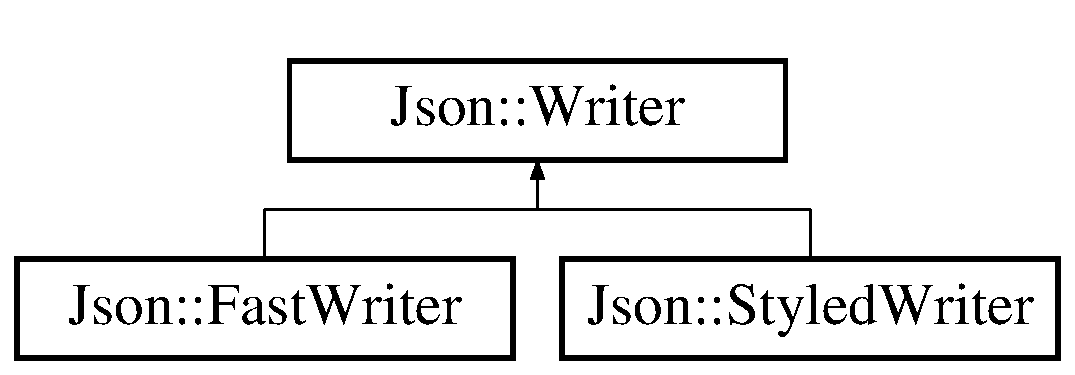
\includegraphics[height=2.000000cm]{class_json_1_1_writer}
\end{center}
\end{figure}
\subsection*{Public Member Functions}
\begin{DoxyCompactItemize}
\item 
virtual std\+::string {\bfseries write} (const \hyperlink{class_json_1_1_value}{Value} \&root)=0\hypertarget{class_json_1_1_writer_a7b2273a4ffd6f32b369ac8a53b7b5a0d}{}\label{class_json_1_1_writer_a7b2273a4ffd6f32b369ac8a53b7b5a0d}

\end{DoxyCompactItemize}


\subsection{Detailed Description}
Abstract class for writers. 

\begin{DoxyRefDesc}{Deprecated}
\item[\hyperlink{deprecated__deprecated000007}{Deprecated}]Use \hyperlink{class_json_1_1_stream_writer}{Stream\+Writer}. (And really, this is an implementation detail.) \end{DoxyRefDesc}


The documentation for this class was generated from the following files\+:\begin{DoxyCompactItemize}
\item 
/home/andrea/\+Clion\+Projects/saas/lib/jsoncpp/inc/json.\+h\item 
/home/andrea/\+Clion\+Projects/saas/lib/jsoncpp/src/jsoncpp.\+cpp\end{DoxyCompactItemize}

%--- End generated contents ---

% Index
\backmatter
\newpage
\phantomsection
\clearemptydoublepage
\addcontentsline{toc}{chapter}{Index}
\printindex

\end{document}
